\documentclass[11pt]{book}

\usepackage{emptypage}

\usepackage[T1]{fontenc}
\usepackage[utf8x]{inputenc}
\usepackage{lmodern}

\usepackage{pdflscape}

\usepackage{listings}
\usepackage[hyperfootnotes=false]{hyperref}
\usepackage{exercise}

\usepackage{algorithm}
\usepackage{algorithmicx}
\usepackage[noend]{algpseudocode}

\usepackage[toc,page]{appendix}

\usepackage[secthm,mdthm]{evan}

\usepackage{answers}

\lhead{Hsiang, Wei, Liu}

\usepackage{graphicx}

\usepackage{color}

\definecolor{myseagreen}{RGB}{88,197,191}
\definecolor{mysalmon}{RGB}{255,160,122}
\definecolor{myred}{RGB}{255,102,102}
\definecolor{mypurple}{RGB}{225,145,255}
\definecolor{myblack}{RGB}{0,0,0}
\definecolor{mywhite}{RGB}{255,255,255}

\usepackage{tikz}

\usetikzlibrary{calc,shapes.multipart,chains,arrows,positioning}

\tikzstyle{vertex}=[draw,fill=myseagreen,circle,minimum size=24pt,inner sep=0pt]

\tikzstyle{splitvertex}=[draw,fill=myseagreen,circle split,minimum size=24pt]

\usetikzlibrary{
  shapes.multipart,
  matrix,
  positioning,
  shapes.callouts,
  shapes.arrows,
  shapes.geometric,
  decorations.shapes,
  shapes,
  fit,
  arrows,
  positioning,
  trees,
  mindmap,
  calc}

\tikzset{
    squarecross/.style={
        draw, rectangle,minimum size=18pt, fill=myseagreen,
        inner sep=0pt, text=black,
        path picture = {
            \draw[black]
            (path picture bounding box.north west) -- 
            (path picture bounding box.south east)
            (path picture bounding box.south west) -- 
            (path picture bounding box.north east);
        }
    }
}

\lstset{language=Java}
 
\definecolor{codegreen}{rgb}{0,0.6,0}
\definecolor{codegray}{rgb}{0.5,0.5,0.5}
\definecolor{codepurple}{rgb}{0.58,0,0.82}
\definecolor{backcolour}{rgb}{0.95,0.95,0.92}

\lstnewenvironment{mylstlisting}[1][]%
  {\noindent\minipage{\linewidth}\medskip 
   \lstset{
    backgroundcolor=\color{backcolour},   
    commentstyle=\color{codegreen},
    keywordstyle=\color{magenta},
    numberstyle=\tiny\color{codegray},
    stringstyle=\color{codepurple},
    basicstyle=\footnotesize,
    breakatwhitespace=false,         
    breaklines=true,                 
    captionpos=t,                    
    keepspaces=true,                 
    numbers=left,                    
    numbersep=5pt,                  
    showspaces=false,                
    showstringspaces=false,
    showtabs=false,                  
    tabsize=4,
   basicstyle=\ttfamily\footnotesize,
   frame=single,#1}}
  {\endminipage}

\raggedbottom

\usepackage{footnote}
\makesavenoteenv{tabular}
\makesavenoteenv{table}

\renewcommand{\arraystretch}{1.5}

% \includeonly{chapters/standard_ds}

\begin{document}

\frontmatter

\title{Crash Course Coding Companion}
\author{
Samuel Hsiang \\ 
Thomas Jefferson High School for Science and Technology \\ 
\href{mailto:samuel.c.hsiang@gmail.com}{\texttt{\textup{samuel.c.hsiang@gmail.com}}} \\
\vspace{.7em}
Alexander Wei \\
Phillips Exeter Academy \\
\vspace{.7em}
Yang Liu \\
Massachusetts Institute of Technology
}
\date{\today}

\maketitle

\newpage
~\vfill
\thispagestyle{empty}

% \noindent Copyright \copyright\ 2013 John Smith\\ % Copyright notice

\noindent Copyright, publishing, and licensing information should go here. I don't have anything fancy like that. It is of my (na\"{i}ve, privileged teenager) belief that knowledge should be free and easily accessible to ambitious high schoolers, but it is paramount to respect intellectual property and someone else's work. I ask that you use this material to its fullest potential, however you like, provided it doesn't completely butcher the philosophy with which I embarked on this project.

\begin{flushright}
-- Samuel
\end{flushright}

% \noindent \textsc{Published by Publisher}\\ % Publisher

% \noindent \textsc{book-website.com}\\ % URL

\noindent \url{https://www.dropbox.com/s/z2lur71042pjaet/guide.pdf?dl=0}

\noindent \url{https://github.com/alwayswimmin/cs_guide}

% \noindent Licensed under the Creative Commons Attribution-NonCommercial 3.0 Unported License (the ``License''). You may not use this file except in compliance with the License. You may obtain a copy of the License at \url{http://creativecommons.org/licenses/by-nc/3.0}. Unless required by applicable law or agreed to in writing, software distributed under the License is distributed on an \textsc{``as is'' basis, without warranties or conditions of any kind}, either express or implied. See the License for the specific language governing permissions and limitations under the License.\\ % License information

% \noindent \textit{First printing, March 2013} % Printing/edition date

\newpage
\thispagestyle{empty}
% \par\vspace*{.35\textheight}{\centering For Rachel \par}


\include{chapters/acknowledgments}

\tableofcontents

\listofalgorithms

\chapter{Preface}

You might have heard of \href{https://www.dropbox.com/s/z8qdndxmrmxqsam/Napkin.pdf?oref=e&n=97419869}{Evan Chen's Napkin}, a resource for olympiad math people that serves as a jumping point into higher mathematics.\footnote{In fact, I'm using Evan's template right now. Thanks Evan!} The Wikipedia articles on higher mathematics are just so dense in vocabulary and deter many smart young students from learning them before they are formally taught in a course in college. Evan's Napkin aims to provide that background necessary to leap right in.

I feel the same way about computer science. For most, the ease of the AP Computer Science test means that the AP coursework is often inadequate in teaching the simplest data structures, algorithms, and big ideas necessary to approach even silver USACO problems. On the other hand, even the best reference books, like Sedgewick, are too dense and unapproachable for someone who just wants to sit down and learn something interesting.\footnote{Sedgewick, notably, is getting better. \href{http://algs4.cs.princeton.edu/home/}{Check out his online companion} to \textit{Algorithms, 4th Edition}.} The road, for many, stalls here until college. Everyone should be able to learn the simplest data structures in Java or C++ standard libraries, and someone with problem-solving experience can easily jump right into understanding algorithms and more advanced data structures.

A few important notes, before we begin.

\begin{itemize}

\item

I'm assuming some fluency in C-style syntax. If this is your first time seeing code, please look somewhere else for now.

\item

It is essential that you understand the motivations and the complexities behind everything we cover. I feel that this is not stressed at all in AP Computer Science and lost under the heavy details of rigorous published works. I'm avoiding what I call the heavy details because they don't focus on the math behind the computer science and lose the bigger picture. My goal is for every mathematician or programmer, after working through this, to be able to code short scripts to solve problems. Once you understand how things work, you can then move on to those details which are necessary for building larger projects. The heavy details become meaningless as languages develop or become phased out. The math and ideas behind the data structures and algorithms will last a lifetime.

\item

It is recommended actually code up each data structure with its most important functions or algorithm as you learn them. I truly believe the only way to build a solid foundation is to code. Do not become reliant on using the standard library (\texttt{java.util}, for instance) without understanding how the tool you are using works.

\end{itemize}


\mainmatter

\chapter{Fundamentals}

\section{Introduction}

Welcome to competitive programming! If you know a bit about coding and you're curious about programming contests, then you're in the right place. We'll start these notes with some basic background: what happens during a programming contest, which skills they train, and how to practice and become better. In the second part of this section, we'll walk through an example contest problem together.

As you move forward, these notes will both guide you through key algorithmic and data structural ideas and provide interesting problems for you to think about. We'll try to challenge you, make you a better problem solver and programmer, and give you a sense for how the foundational concepts in computer science are intricately connected. The skills you'll pick up will be useful in not just other areas of computer science, but will also make you a stronger and more creative thinker. If you have questions or feedback about anything as you go along, feel free to contact us at \mailto{@gmail.com}. We hope you'll enjoy the world of competitive programming as much as we have. Have fun with it!

\subsection{What is Competitive Programming?}

A programming contest typically consists of a collection of problems and a time limit within which they must be solved. To solve a problem, you'll have to code a program that reads some parameters as input and produces an output of the desired format. You'll then submit your code to a \emph{judging server}, which is a server that compiles your code and executes it on a set of \emph{test cases}. To pass, your program must solve each test case using only predetermined amounts of \emph{time} and \emph{memory}. That is, your program must be \textit{efficient}. Furthermore, your program must be \textit{correct}. To check correctness, the output for each test case is either compared to the output of a correct program written by the contest organizers or plugged into a verifier that checks that your output satisfies the desired conditions. So as a contestant, your job will be to find an efficient algorithm, write correct code, and submit.

This is just a very general description of programming contests. Each contest has its particularities in terms of scoring and the feedback you get on your submissions. Some contests will only mark your submission as correct if it correctly solves every test case, while others will give you partial credit for every test case you get correct.  Some contests will also execute your submissions in real time, so you'll know if your code is correct within seconds, while others will only judge your final submissions after the contest is over. But the commonalities of these contests are in the skills they select for and train.

Problem solving is possibly the most important skill you can learn. This skill, and not whether you can crank out code quickly, is what interesting programming contests are about. You'll be given problems you'll have no idea how to solve, and you'll want to creatively reason about these problems and discover efficient solutions. Of course, being able to write clean, accurate code is also of high importance, since it is your code, not the solution in your head, that gets judged. For programming language, we recommend (and our notes will cover) coding in \emph{Java} or \emph{C++}. Finally, a solid understanding of algorithms and data structures will give you the tools you'll need to crack these problems. This combination of problem solving, coding, and algorithmic thinking will get you a long way in programming contests, and you'll definitely be able to apply them elsewhere too.

We'll do our best to teach you these skills by providing you with notes that show you the important algorithmic and data structural ideas, giving you pointers on how to write code, and presenting you with problems that will solidify your knowledge. I cannot emphasize how important solving the problems and writing the code is for your growth. Try to avoid reading solutions until you've given the problem a genuine shot and feel like you've stopped making progress. And if you do read a solution, think about how you'll be able to solve a similar problem the next time it appears. After you solve a problem, code it up, and don't give up trying to fix and optimize your code until you get all test cases accepted. Think of each bug you find as another bug you'll never see again.

But there is only so much we can do. The challenging part---persevering with difficult problems, spending long hours spent debugging, and taking time from your busy day to code---is all on you.

\subsection{First Problem: Sliding Puzzles}

We'll now work through an example problem, adapted from a recent Codeforces contest. On the next page is a typical problem statement, with the problem description followed by input and output specifications and sample cases. Try to come up with a solution (and possibly write some code) before reading our analysis. As in the rest of these notes, we'll follow our analysis with some discussion of how to implement the solution and provide links to C++ and/or Java code.

\clearpage

\statement[Sliding Puzzles]{2s}{256MB}{%
  Bessie and her best friend Elsie each own a sliding puzzle. Each of their sliding puzzles consists of a $2\times 2$ grid and three tiles labeled $\mathcal A$, $\mathcal B$, and $\mathcal C$. The three tiles sit on top of the grid, with one grid cell left empty. To make a move, one slides a tile adjacent to the empty cell into the empty cell, as shown below:
  \begin{center}
    \includegraphics[scale=0.6]{images/sliding-puzzle.png}
  \end{center}
  Bessie and Elsie would like to know if there exists a sequence of moves that takes their puzzles to the same configuration. (Moves can be performed on both puzzles.) Two puzzles are considered to be in the same configuration if each tile is on top of the same grid cell in both puzzles. Since the tiles are labeled with letters, rotations and reflections are not allowed.
}{%
  The first two lines of the input consist of a $2\times 2$ grid describing the initial configuration of Bessie's puzzle. The next two lines contain a $2\times 2$ grid describing the initial configuration of Elsie's puzzle. The positions of the tiles are labeled $\mathtt A$, $\mathtt B$, and $\mathtt C$, while the empty cell is labeled $\mathtt X$. It is guaranteed that the input contains two valid descriptions of puzzles.
}{%
  Print \texttt{YES} if the puzzles can reach the same configuration. Otherwise, print \texttt{NO}.
}{\href{http://codeforces.com/contest/645/problem/A}{Codeforces 645A}}
\sample{%
  AB
  XC
  XB
  AC%
}{YES}
\sample{%
AB
XC
AC
BX%
}{NO}

\clearpage

We present two solutions to this problem. The first is the more ``obvious'' one, while the second shows how solutions can often be simplified through some thinking and some clever observations.

\begin{proof}[Solution 1]
  One straightforward approach to this problem is to notice that there are only $4! = 24$ possible  configurations that a puzzle could be in. Thus, for each puzzle in the input, it shouldn't be hard to find the list of configurations that the puzzle can reach. Once we have the lists of configurations, we can compare the two lists and check if they have an element in common. If they do, we output $\mathtt{YES}$; otherwise, we output $\mathtt{NO}$.

  To find the list of possible configurations, we maintain a list containing all of the possible configurations we have found so far. (This list starts off as the puzzle itself.) For every configuration in our list, we check if a single move can take us to a configuration we haven't seen before. Once we find a new configuration, we append it to the list and repeat. If there exist no such new configurations, then our list contains all possible configurations for that puzzle.
\end{proof}

However, this solution may be somewhat difficult to implement---we have to figure out how to nicely represent each configuration as a string and make moves to reach new configurations. Writing the code to find the list of possible configurations is also a bit complex. Instead, a simple observation can reduce the trickiness of the code significantly:

\begin{proof}[Solution 2]
  Notice that two puzzles can reach the same configuration if and only if the $\mathcal A$, $\mathcal B$, and $\mathcal C$ tiles appear in the same orientation---clockwise or counterclockwise---in the two puzzles. Thus, it suffices to check if the two puzzles have the same orientation. We can do so by writing down the tiles of each puzzle in clockwise order and checking if one string is a cyclic shift of the other.
\end{proof}

To implement the first solution, you might want to make your list of possible configurations a \emph{dynamic array}---that is, a Java \texttt{ArrayList} or a C++ \texttt{vector}. This will allow you to easily append elements to the list.

For the second solution, once we have the tiles in clockwise order, we'll want to check if one ordering is a cyclic shift of the other. Given two strings $s$ and $t$ of the same length, a clever way to do this is to check if $s$ is a substring of $t+t$. (Convince yourself that this is correct!) Take a look at a \href{http://codeforces.com/contest/645/submission/16801722}{C++} implementation of Solution 2 using this trick.

\section{More Problems!}
\label{sec:moreproblems}

Because problems are the most important thing in the world, below are a couple more for you to chew on. We'll cover solutions to these problems later in the chapter, but if you feel ready, try submitting your code on \href{http://codeforces.com}{Codeforces} first.

\statement[Vasily and Candles]{1s}{256MB}{%
  Vasily the programmer loves romance, so he plans to write code while bathed in the warm glow of candlelight. He has $a$ new candles, each of which burns for exactly one hour. Vasily is smart, so he can make a new candle from $b$ burnt out candles. Vasily wonders, for how many hours can his candles light up his room if he acts optimally?
}{%
  The input contains two integers, $a$ and $b$ ($1\le a\le 1000$ and $2\le b\le 1000$).
}{%
  Print a single integer---the maximum number of hours for which Vasily's candles can keep his room lit.
}{\href{http://codeforces.com/problemset/problem/379/A}{Codeforces 379A}}
\sample{4 2}{7}
\sample{6 3}{8}

\statement[Kefa and First Steps]{2s}{256MB}{%
  Kefa has started an Internet business $n$ days ago. On the $i$-th day $(1\le i\le n)$, he made a profit of $a_i$ dollars. Kefa loves progress, so he wants to know the length of the longest non-decreasing subsegment in her sequence of profits. (Here, a subsegment of a sequence denotes a contiguous subsequence $a_i,a_{i+1}\ldots,a_j$ ($i < j$).)
}{%
  The first line contains an integer $n$ ($1\le 10^5$). The second line contains $n$ integers $a_1,a_2,\ldots,a_n$ ($1\le a_i\le 10^9$).
}{%
  Print a single integer--the length of the maximum non-decreasing sequence in Kefa's profits.
}{\href{http://codeforces.com/problemset/problem/580/A}{Codeforces 580A}}
\sample{%
  6
  2 2 1 3 4 1%
}{3}
\sample{%
  3
  2 2 9%
}{3}

\section{Input and Output}

Now that you've familiarized yourself with what programming contest problems are like, let's get down to the details. The first part of solving any problem is reading the input correctly. As you may expect, doing so is very dependent on programming language. In this section, we'll cover input and output (I/O) in both Java and C++. Read our discussion for whichever one you plan to use.

\subsection{Java}
Here, we'll focus on Java I/O using \texttt{java.util.Scanner} and \texttt{java.io.PrintWriter}. There are two scenarios that you should be familiar with: standard I/O and file I/O. That is, interacting with \texttt{System.in/System.out} and files like \texttt{in.txt/out.txt}, respectively. You may have encountered standard I/O when you enter input and see output while running a program in the command line.

When using standard I/O, we can read from \texttt{System.in} using \texttt{java.util.Scanner} and output using \texttt{System.out.println}. To declare a new Scanner, simply call the constructor with \texttt{new Scanner(System.in)}. Here's a quick outline of Scanner methods:
\begin{center}
  \begin{tabularx}{0.75\textwidth}{|l|X|}
    \hline
    Method & Description \\ \hline
    \texttt{Scanner.next()} & Reads the next token in the input (i.e. up to a whitespace) and returns the token as a \texttt{string}. \\ \hline
    \texttt{Scanner.nextLine()} & Reads the input up to a line break and returns the contents read as a \texttt{string}. \\ \hline
    \texttt{Scanner.nextInt()} & Reads the next token in the input (i.e. up to a whitespace) and returns the token as an \texttt{int}. \\ \hline
    \texttt{Scanner.nextLong()} & Reads the next token in the input (i.e. up to a whitespace) and returns the token as an \texttt{long}. \\ \hline
    \texttt{Scanner.nextDouble()} & Reads the next token in the input (i.e. up to a whitespace) and returns the token as an \texttt{double}. \\ \hline
  \end{tabularx}
\end{center}
\texttt{System.out.println()} prints its argument and adds a newline at the end. (If you don't want the newline, you can use \texttt{System.out.print()}.) Here's an example of a \texttt{main} method that takes two integers and outputs their sum:

\begin{mylstlisting}
public static void main(String args[]) {
  // hint: you should have "import java.util.*;" at the top of your code.
  Scanner sc = new Scanner(System.in);
  int x = sc.nextInt();
  int y = sc.nextInt();
  System.out.println(x + y);
}
\end{mylstlisting}

File I/O is a touch more complicated. For our Scanner, we now have to call the constructor with a File object (e.g. with \texttt{new File("in.txt")}). We do the same with output for our PrintWriter (e.g. with \texttt{new File("out.txt")}). We can then use PrintWriter like we use \texttt{System.out}, by calling \texttt{pw.println()} and \texttt{pw.print()} for a PrintWriter \texttt{pw}.

However, PrintWriter also comes with a couple more usage notes. First, we should include \texttt{throws IOException} after our \texttt{main} method, since Java requires that we acknowledge the possibility of an \texttt{IOException} in the case that something goes wrong. After we finish printing, we must also close the PrintWriter in order to ensure that everything gets written to the file. Here's a snippet showing how Scanner and PrintWriter work together with files: 

\begin{mylstlisting}
public static void main(String args[]) throws IOException {
  // hint: for file I/O, you should also have "import java.io.*;"
  Scanner sc = new Scanner(new File("in.txt"));
  int x = sc.nextInt();
  int y = sc.nextInt();
  PrintWriter pw = new PrintWriter(new File("out.txt"));
  pw.println(x + y);
  pw.close();
}
\end{mylstlisting}

Although more efficient methods of I/O exist, such as BufferedReader and BufferedWriter, what we've covered here should be sufficient for now. For example, it is possible to read $10^5$ integers with Scanner in a fraction of a second.

\subsection{C++}

Here, we discuss I/O in C++ using the Standard Template Library's (STL) \texttt{iostream} and \texttt{fstream}. There are two scenarios that you should be familiar with: standard I/O and file I/O. You may have encountered standard I/O when you enter input and see output while running a program in the command line, whereas file I/O involves reading from and writing to files like \texttt{in.txt} or \texttt{out.txt}. In C++, standard I/O is done with the \texttt{cin} and \texttt{cout} objects in \texttt{iostream}, and file I/O is done with the \texttt{ofstream} and \texttt{ifstream} classes in \texttt{fstream}. We'll go through each of these below.

Using \texttt{cin} and \texttt{cout} is pretty straightforward. If you have a variable \texttt{x} that you want to read input into, you can do so by writing \verb+cin >> x+. If \texttt{x} is an \texttt{int}, \texttt{double}, or \texttt{long long}, this will read the next such number in the input (up to a whitespace) into \texttt{x}. If \texttt{x} is a string, then \texttt{cin} will read similarly the input up to a whitespace into \texttt{x}. To output a variable \texttt{x} that is of type \texttt{int}, \texttt{double}, \texttt{long long}, \texttt{string}, or \texttt{bool}, we simply write \verb+cout << x+. To output a newline, you can write \verb+cout << endl+. And that's all!

Here's an example with \texttt{cin} and \texttt{cout} that outputs the sum of two integers:

\begin{mylstlisting}
int main() {
  // hint: you should have "#include <iostream>" at the top of your code.
  int x, y;
  cin >> x >> y;
  cout << x + y << endl;
}
\end{mylstlisting}

Moving on to file I/O, suppose we want to read from \texttt{in.txt} and write to \texttt{out.txt}. We construct an \texttt{ifstream} and an \texttt{ofstream} on \texttt{in.txt} and \texttt{out.txt}, respectively. We can do so by writing \texttt{ifstream fin("in.txt")} and \texttt{ofstream fout("out.txt")}. Then \texttt{fin} and \texttt{fout} behave just like \texttt{cin} and \texttt{cout}. Here's an example:

\begin{mylstlisting}
int main() {
  // hint: you should have "#include <iostream>" at the top of your code.
  ifstream fin("in.txt");
  ofstream fout("in.txt");
  int x, y;
  fin >> x >> y;
  fout << x + y << endl;
}
\end{mylstlisting}

Although more efficient methods of I/O exist, such as \texttt{scanf} and \texttt{printf}, what we've covered here should be sufficient for now. For example, it is possible to read $10^5$ integers with \texttt{cin} and \texttt{cout} in a fraction of a second.

\section{Complexity}

Before, we mentioned that contest problems test your ability to come up with efficient algorithms and to write accurate code. \emph{Implementation problems} are problems that for the most part, assess the latter---that is, your ability to write code quickly and accurately. However, these problems are usually only common in easier contests, since they don't involve too much thinking or creativity; you just have to carefully implement what's written in the problem statement. Instead, most competitive programming problems ask you to come up with clever algorithms that are both fast and space-efficient.

To formally analyze the efficiency of algorithms, computer scientists use the notion of \emph{complexity}. Complexity is roughly the number of steps an algorithm takes as a function of the input size. You can imagine algorithms that require $3n$, $n^4/3$ or even $2^n + n^2$ steps to halt for an input of size $n$. We categorize algorithms of different complexities using \emph{big-O notation}: If an algorithm takes $f(n)$ steps to halt on an input of size $n$, we say that the algorithm is $O(f(n))$. However, this notation ignores any constant factors and lower-order terms in the expression. For example, an algorithm that requires $100n^2 + 5$ steps is still $O(n^2)$.\footnote{Actually, this isn't entirely accurate. Saying an algorithm is $O(f(n))$ really means that there exists a $c > 0$ such that the algorithm takes \emph{at most} $c\cdot f(n)$ steps to halt.} I'll explain why in a moment---let's look at some examples for now. 

Suppose we have three programs $A$, $B$, and $C$ that require $3n$, $n^4/3+10$ and $2^n + n^2$ steps to finish, respectively. The complexity of the program A$A$ is $O(n)$ because we ignore the constant factor $3$ on the $3n$. The complexity of the program $B$ is $O(n^4)$. Here, we drop the constant $1/3$ and the lower-order term $10$. For program $C$, we write its complexity as $O(2^n)$ because $n^2$ is a lower-order term relative to $2^n$.

As to why we drop the constants and the lower order terms, consider programs $A$ and $B$ from above. When $n=300$, the first program takes $900$ steps, while the second program takes $2,700,000,010$ steps. The second program is much slower, despite a smaller constant factor. Meanwhile, if we had another program that runs in $5n$ steps, it would still only take $1,500$ steps to finish. Notice how the $10$ after $n^4/3$ also looks irrelevant here. The takeaway is that constant factors and lower-order terms get dwarfed when comparing functions that grow at different rates. 

Thus in programming contests, we usually want a program to have a sufficiently good complexity, without worrying about too much constant factors. Complexity will be the difference between whether a program gets \emph{\color{green}accepted} or \emph{\color{red}time limit exceeded}. As a rule of thumb, a modern processor can do around $10^8$ computations each second. When you plug the maximum possible input into the complexity of your algorithm, it should never be much more than that.

We've focused on time and haven't talked much about memory so far, but memory can also be tested. However, in contests, memory limits are usually much more generous than time limits. The amount of memory a program uses as a function of $n$ is called its \emph{space complexity}, as opposed to the \emph{time complexity} that we discussed earlier. If a program uses $2n^2$ bytes of memory on an input of length $n$, then it has a space complexity of $O(n^2)$.

\section{More Solutions}

% Now that you know the basics, let's get started by solving a few problems. Try to figure out a solution to each problem before reading our analysis. To test your code for the problems in this chapter, you should create an account on Codeforces. After you login, there will be an ``Introduction'' problem set available \href{http://codeforces.com/group/5tN48zOVvQ/contests}{here} that includes these problems and a few extras.

Have you given the problems from \ref{sec:moreproblems} a shot yet and submitted some code? If you haven't, do so before reading the solutions below.

\subsection{Vasily and Candles}

\begin{proof}[Solution]
  Vasily and Candles is a straightforward implementation problem. Since $a$ and $b$ are small, we can simulate Vasily's candle burning process. We track the number of candles we have left, the number of burnt out candles, and the number of hours that have passed. Whenever we have more than $b$ burnt out candles, we make a new candle. Once we run out of candles, we print the answer. In terms of implementation, a \texttt{while} loop is handy here.
\end{proof}

\subsection{Kefa and First Steps}

\begin{proof}[Solution]
Our first thought upon reading this problem might be to check each subsegment of the sequence $a_i$ and see if that subsegment is non-decreasing. Unfortunately, this is too slow: There are approximately $n^2/2$ pairs of endpoints that we could choose, far too many when $n$ can be up to $10^5$. (Recall that the maximum number of computations we can do is \textasciitilde$10^8$.) Instead, we can solve this problem in $O(n)$ by executing a single \texttt{for} loop over the sequence. We maintain a counter representing Kefa's current ``streak''---the number of days since her profit last decreased. If her profit decreases from day $i$ to day $i+1$, then we reset the counter to zero. The answer we report is the longest streak that we ever see.
\end{proof}

This problem is a clear example of how getting the right complexity is essential. Our initial idea, which could have been implemented in $O(n^3)$ or $O(n^2)$, was too slow. To make our program finish within time limit, we had to come up with a more efficient approach that runs in $O(n)$.

\section{Even More Problems}

For some more fun, check out the rest of the \href{http://codeforces.com/group/5tN48zOVvQ/contest/204614}{Introduction} problem set that we put together on Codeforces. These problems will familiarize you with the essentials of contest programming---algorithmic thinking and writing accurate code. Enjoy!

\begingroup
\chapter*{Interlude A}
\addcontentsline{toc}{chapter}{Interlude A}
% \renewcommand\thesection{\Alph{chapter}.\arabic{section}}
% \setcounter{section}{0}

\section{Sorting}

To further explore the concept of complexity, we will use sorting algorithms as a case study. Sorting is just as it sounds---given a collection of objects, we want to sort them according to some ordering. For example, suppose we have a list of scores from a programming contest. In order to generate the final standings, we'll need to sort the contestants in descending order by score. Below, we present three classic sorting algorithms of varying complexity: insertion sort, merge sort, and quicksort. Insertion sort runs in $O(n^2)$, while merge sort and quicksort both run in $O(n\log n)$.

Don't worry too much about the details of these algorithms for now. You'll rarely need to implement them from scratch, since almost all modern programming languages come with built-in sorting algorithms. In our last subsection, we'll provide an example using these library functions in Java and C++ by working through a problem for which sorting is a subtask.

% To supplement our descriptions of the algorithms, you can check out the animations at \url{http://visualgo.net/sorting.html}.

\subsection{Insertion Sort}

Insertion sort builds up a sorted list by inserting new elements one at a time. Inserting an element into a sorted list can be done in time proportional to the length of the list, so the runtime of this algorithm is $1 + 2 + 3 + \cdots + n = (n^2 + n) / 2$, which is $O(n^2)$. Here's some pseudo code for insertion sort:

Notice that after the $i$-th iteration, we have a sorted list in the first $i$ entries of the array. Insertion sort, despite being slower than merge sort and quicksort, is still useful because of its efficiency on small inputs. Many implementations of merge sort and quicksort actually use insertion sort once the problem size gets small.

\begin{exercise}
  Around how long is the longest list that you can sort with insertion sort in less than a second?
\end{exercise}

\subsection{Merge Sort}

The idea behind merge sort is the observation that given two sorted lists of length $n/2$, we only need $n$ comparisons to merge them into a single sorted list of length $n$. We merge the two lists as follows: First, it is easy to find the smallest element among the two lists, since this element has to be the smallest element in one of the lists. To find the second-smallest element, we can delete the smallest element and do the same comparison again.

This method of merging lists allows us to sort using a divide and conquer approach. We split the array in half, sort each half recursively with merge sort, and then merge the two halves back together. Because our recursion goes $\log_2 n$ levels deep and requires $O(n)$ operations per level, this algorithm runs in $O(n \log n)$. (In fact, it is possible to prove that $O(n \log n)$ is optimal for comparison-based sorting algorithms, one of the few problems in computer science that has a non-trivial lower bound.)

\begin{exercise}
  Around how long is the longest list that you can sort with merge sort in less than a second?
\end{exercise}

\subsection{Quicksort}

Quicksort also uses a divide and conquer strategy to run in $O(n \log n)$ on average. We first choose a random element from the array and call it the \emph{pivot}. We rearrange the array so that anything less than the pivot to the left of the pivot and anything greater than the pivot to the right of the pivot. This rearranging can be done in $O(n)$. Like merge sort, we can then recursively quicksort the two ``halves'' of the array defined by the pivot. Since we chose the pivot randomly, our problem size gets reduced down by a factor of $3/4$ most of the time, giving us $O(\log n)$ levels of recursion with $O(n)$ operations at each level. Thus quicksort runs in $O(n \log n)$ on average. We say ``on average'' because there do exist cases that make quicksort run in $O(n^2)$.

\begin{exercise}
  What would happen if we chose the smallest element of the array as the pivot each time?
\end{exercise}

\subsection{Sorting Applied}

\statement[Ms. Manana's Puzzles]{1s}{256MB}{%
  The end of the school year is near and Ms. Manana, the teacher, will soon have to say goodbye to yet another class. As a farewell present, she decides to give each of here $n$ students a jigsaw puzzle. The shop asssistant tells Ms. Manana that there are $m$ puzzles in the shop, but they differ in difficulty and size. Specifically, the $i$-th jigsaw puzzle consists of $f_i$ pieces. Ms. Manana doesn't want to upset the children, so she wants the difference between the numbers of pieces in the largest puzzle and the smallest puzzle that she buys to be as small as possible. Help Ms. Manana compute this minimum difference.
}{%
  The first line contains space-separated integers $n$ and $m$ ($2\le n\le m\le 50$). The next line contains $m$ space-separated integers $f_1,f_2,\ldots,f_m$ ($4\le f_i\le 1000$).
}{%
  Print a single integer---the least possible difference that Ms. Manana can obtain.
}{\href{http://codeforces.com/problemset/problem/337/A}{Codeforces 337A}}
\sample{%
  4 6
  10 12 10 7 5 22
}{5}

\begin{proof}[Solution]
  We solve this problem by first sorting the sequence $f_i$. After sorting, Ms. Manana will want to buy puzzles from a contiguous block of the sequence. (If she doesn't, then the difference between the largest and smallest puzzles will be greater than necessary.) Thus we can iterate through the sorted sequence to find the minimum difference between the endpoints of each subsegment of length $n$.
\end{proof}

Usually, when solving a sorting problem, we don't need to implement our own sorting function. Java users have \texttt{Arrays.sort} in \texttt{java.utils.Arrays} that does the magic for you. For those who code in C++, if you \texttt{\#include <algorithm>}, you can then use \texttt{std::sort}. While coding up Ms. Manana's Puzzles, try to use the library sort function in your language.

Here are code snippets for sorting an array \texttt{arr} of length \texttt{n} in Java and C++, respectively:

\begin{mylstlisting}
// hint: you should have "import java.util.*;" at the top of your code.
int[] arr = new int[n];
// do something to fill up the array.
Arrays.sort(arr);
\end{mylstlisting}

\begin{mylstlisting}
// hint: you should have "#include <algorithm>" at the top of your code.
int arr[n];
// do something to fill up the array.
std::sort(arr, arr + n);
\end{mylstlisting}
\endgroup


\chapter{Standard Library Data Structures}
\label{chap:standard_ds}

The purpose of this chapter is to provide an overview on how the most basic and useful data structures work. The implementations of most higher-level languages already coded these for us, but it is important to know how each data structure works rather than blindly use the standard library.

More technical explanations of all of these can be found in a language's API. For Java, this is mostly under the package \texttt{java.util}, in the \href{https://docs.oracle.com/javase/8/docs/api/}{Java API}.

I strongly believe that Java is better than C++ for beginning programmers. It forces people into good coding habits, and though the lack of pointers initially frustrated me, it really does make learning general concepts liked LinkedLists much easier, as the intricacies of the C++ pointer no longer distract from the larger idea.

\section{Generics}
\label{sec:generics}

In general, a data structure can store any kind of data, ranging from integers to strings to other data structures. We therefore want to implement data structures that can hold any and all kinds of information. When we use a data structure, however, we might want our structure to store only one kind of information: only strings, for example, or only integers. We use \textit{generics} to specify to an external structure that we only want it to store a particular kind of information.

\begin{mylstlisting}
ArrayList<Integer> al = new ArrayList<Integer>();
\end{mylstlisting}

This means that \texttt{al} is an ArrayList of Integers. We can only add Integers into the ArrayList, and anything removed from the ArrayList is guaranteed to be an Integer. We can write \texttt{Integer i = al.get(0)} without any need to cast to an Integer.

I don't think the beginning programmer needs to know how to necessarily code a class that supports generics, since each language has its own complex set of rules governing generics. However, we use the standard library extensively in any coding environment, so it is necessary to use a class that does support generics. I think standard classes are relatively straightforward to use but can be annoying to actually implement.

When examining a language's API or explanations of implemented functions in this chapter, the characters \texttt{E}, \texttt{V}, and \texttt{K} represent generic classes. For example, when we set \texttt{al = new ArrayList<Integer>()}, \texttt{E} represents \texttt{Integer}. Otherwise, \texttt{E} simply means any object.

\section{List}

A List is a collection of objects with an ordering. Users of a list have control over where in the list each object is and can access a specific element by its index, like in an array.

\subsection{Size-Adjustable Array}

What is nice about an array? We can access or change any element we want in the array in $O(1)$ time. The problem is that an array has fixed length. It's not easy to append an element to the end of an array.

The fix to this is pretty simple. Why not just make a bigger array, and copy everything over to the new array? Then there's more room at the end to add a new element. If the backbone array runs out of space, we create a new array with double the size and keep going as if nothing happened.

\begin{center}
{
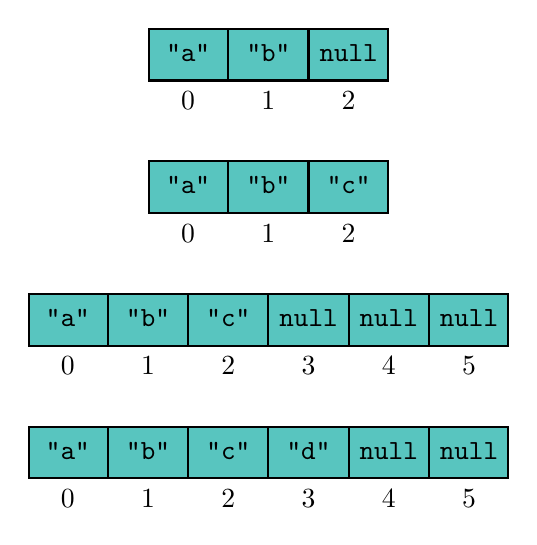
\begin{tikzpicture}[
  thick,
  myrect/.style={
    draw,
    fill=myseagreen,
    rectangle split,
    rectangle split horizontal,
    rectangle split parts=#1,
    rectangle split part align=left,
    text width=5ex,
    text centered
    },
  mycallout/.style={
    shape=rectangle callout,
    rounded corners,
    fill=mysalmon,
    callout absolute pointer={#1},
    callout pointer width=1cm
  }  
]

\node[myrect=3]
  (array1)
  {
  					\strut \texttt{"a"}
  \nodepart{two}	\strut \texttt{"b"}
  \nodepart{three}	\strut \texttt{null}
  };
\foreach \Valor [count=\Valori from 0] in {one ,two ,three }
  \node[below] at (array1.\Valor south) {\Valori};

\node[myrect=3]
  (array2)[below=of array1]
  {
  					\strut \texttt{"a"}
  \nodepart{two}	\strut \texttt{"b"}
  \nodepart{three}	\strut \texttt{"c"}
  };
\foreach \Valor [count=\Valori from 0] in {one ,two ,three }
  \node[below] at (array2.\Valor south) {\Valori};

\node[myrect=6]
  (array3)[below=of array2]
  {
  					\strut \texttt{"a"}
  \nodepart{two}	\strut \texttt{"b"}
  \nodepart{three}	\strut \texttt{"c"}
  \nodepart{four}	\strut \texttt{null}
  \nodepart{five}	\strut \texttt{null}
  \nodepart{six}	\strut \texttt{null}
  };
\foreach \Valor [count=\Valori from 0] in {one ,two ,three , four , five , six }
  \node[below] at (array3.\Valor south) {\Valori};

\node[myrect=6]
  (array4)[below=of array3]
  {
  					\strut \texttt{"a"}
  \nodepart{two}	\strut \texttt{"b"}
  \nodepart{three}	\strut \texttt{"c"}
  \nodepart{four}	\strut \texttt{"d"}
  \nodepart{five}	\strut \texttt{null}
  \nodepart{six}	\strut \texttt{null}
  };
\foreach \Valor [count=\Valori from 0] in {one ,two ,three , four , five , six }
  \node[below] at (array4.\Valor south) {\Valori};

\end{tikzpicture}
}
\end{center}

We see that there is still room in the array to add \texttt{"c"}, but to add more elements to the list, we must use a new array with double the length.

It's important to note that any given insertion to the structure is either $O(n)$ or $O(1)$, but there is only one $O(n)$ insertion for every $O(n)$ $O(1)$ insertions, so we still average out to constant time.

\begin{itemize}

\item
\texttt{boolean add(String s)} -- add an element to the end of the list. (By convention, this returns \texttt{true} if the addition was successful, and \texttt{false} otherwise.)
\item
\texttt{void add(int i, String s)} -- shift everything from position \texttt{i} onward down by one, and add \texttt{s} at position \texttt{i}.
\item
\texttt{boolean contains(Object o)} -- return \texttt{true} if \texttt{o} is stored in the ArrayList, and \texttt{false} otherwise. Remember to cast \texttt{o} to a String.
\item
\texttt{String get(int i)} -- return the element stored at index \texttt{i}.
\item
\texttt{boolean isEmpty()} -- return \texttt{true} if \texttt{size() == 0}.
\item
\texttt{String remove(int i)} -- remove and return the element at index $i$ from the list. (Why is this annoying?)
\item
\texttt{String set(int i, String s)} -- replace the element stored at index \texttt{i} with \texttt{s}, and return the element that was originally at position \texttt{i}.
\item
\texttt{int size()} -- note that this is not just the length of the backbone array.
\end{itemize}

The \texttt{get} and \texttt{set} functions are very nice. They are easy to code and run in constant time. These are the bread and butter of any array. Adding at the end of the ArrayList is nice as well. \texttt{contains} is a pain, as it is $O(n)$, and adding to and removing from early in the list are more annoying.

If this is your first time seeing an ArrayList, I would suggest coding up your own. It should be relatively straightforward.

\subsection{LinkedList}

Arrays are nice for accessing, say, the seventh element in the list. We extend this to an ArrayList to implement adding and removing elements to and from the end of the list nicely. Removing elements from the beginning of the list, however, is cumbersome.

The LinkedList attempts to remedy this. It trades $O(1)$ access to any element in the list for an easier way to remove elements from either end of the list easily. Consider a chain of paper clips:

\begin{center}

\includegraphics{images/paper_clip_chain.jpg}\footnote{\url{http://img.thrfun.com/img/078/156/paper_clip_chain_s1.jpg}}

\end{center}

It's easy to add or remove more paper clips from either end of the chain, and from any given paper clip, it's easy to access the paper clip directly previous or next to it in the chain. If we needed the seventh paper clip in the chain, we'd need to manually count, an $O(n)$ operation. However, if we then needed to remove that paper clip from the chain, it wouldn't be that hard, assuming we kept a finger on the seventh paper clip.

The standard library implements a cyclical doubly-linked list, with a dummy head. It looks something like this:

\begin{center}


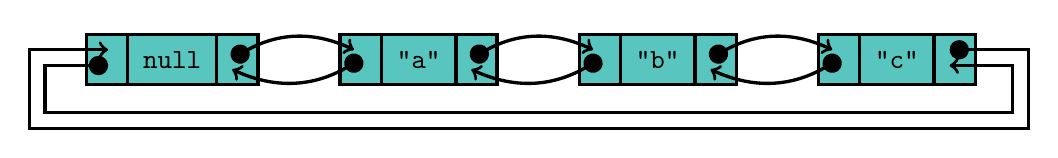
\begin{tikzpicture}[
        list/.style={
            very thick, rectangle split, 
            rectangle split parts=3, draw, 
            rectangle split horizontal, minimum size=18pt,
            inner sep=5pt, text=black,
            rectangle split part fill=myseagreen
        }, 
        ->, start chain, very thick
      ]

  \node[list,on chain] (dummy) {\nodepart{second} \texttt{null}};
  \node[list,on chain] (A) {\nodepart{second} \texttt{"a"}};
  \node[list,on chain] (B) {\nodepart{second} \texttt{"b"}};
  \node[list,on chain] (C) {\nodepart{second} \texttt{"c"}};

    \path[*->] let \p1 = (dummy.three), \p2 = (dummy.center) in (\x1,\y2) edge [bend left] ($(A.one)+(0,0.2)$);
  \path[*->] let \p1 = (A.three), \p2 = (A.center) in (\x1,\y2) edge [bend left] ($(B.one)+(0,0.2)$);
  \path[*->] let \p1 = (B.three), \p2 = (B.center) in (\x1,\y2) edge [bend left] ($(C.one)+(0,0.2)$);
  
%  \draw[*->] let \p1 = (C.three), \p2 = (C.center) in (\x1,\y2) -- (dummy);

%  \draw[*->] ($(A.one)+(0.2,0.1)$) -- (dummy);
  \path[*->] ($(B.one)+(0.1,0.1)$) edge [bend left] ($(A.three)+(0,-0.05)$);
  \path[*->] ($(C.one)+(0.1,0.1)$) edge [bend left] ($(B.three)+(0,-0.05)$);
    \path[*->] ($(A.one)+(0.1,0.1)$) edge [bend left] ($(dummy.three)+(0,-0.05)$);
    
    \draw[*->] ($(C.three)+(0.0,0.2)$) -- ($(C.three)+(1.0,0.2)$) -- ($(C.three)+(1.0,-0.8)$) -- ($(dummy.one)+(-0.9,-0.8)$) -- ($(dummy.one)+(-0.9,0.2)$) -- ($(dummy.one)+(0.1,0.2)$);

    \draw[<-*] ($(C.three)+(0.0,0.0)$) -- ($(C.three)+(0.8,0.0)$) -- ($(C.three)+(0.8,-0.6)$) -- ($(dummy.one)+(-0.7,-0.6)$) -- ($(dummy.one)+(-0.7,0.0)$) -- ($(dummy.one)+(0.1,0.0)$);

\end{tikzpicture}

\end{center}

We see that each node maintains a pointer to its next neighbor and its previous neighbor, in addition to containing the String it stores. We can store this data in a class like the following:

\begin{mylstlisting}
class ListNode {
	ListNode prev, next;
    String s;
}
\end{mylstlisting}

If we were to insert an element after a ListNode \texttt{a}, it is necessary to update all pointers:

\begin{mylstlisting}
ListNode b = new ListNode();
b.prev = a;
b.next = a.next;
b.next.prev = b;
a.next = b;
\end{mylstlisting}

Since the LinkedList is symmetric, inserting an element before a node is also easy. To add something to the end of the list, simply add it before the dummy head. From here it should not be too hard to implement all the important functions of a LinkedList.

\begin{itemize}

\item \texttt{boolean add(String s)} -- add to the end.
\item \texttt{void add(int i, String s)} -- this is linear. Don't forget about 0-indexing.
\item \texttt{void addFirst()}
\item \texttt{boolean contains(Object o)}
\item \texttt{String get(int i)}
\item \texttt{String getFirst()}
\item \texttt{String getLast()}
\item \texttt{boolean isEmpty()}
\item \texttt{String remove()} -- remove the last element.
\item \texttt{String remove(int i)}
\item \texttt{String removeFirst()}
\item \texttt{String set(int i, String s)}
\item \texttt{int size()}

\end{itemize}

With a LinkedList implemented, two other data structures immediately follow.

\section{Stack}

A stack is is literally a stack. If we have a stack of papers, we can \textit{push} things on the top and \textit{pop} things off the top. Sometimes we \textit{peek} at what's on the top but don't actually remove anything. We never do anything with what's on the bottom. This is called \textit{LIFO}: Last In, First Out.

\begin{itemize}

\item \texttt{String push(String s)} -- pushes the item on the top of the stack, and returns the same element.

\item \texttt{String pop()} -- removes the item at the top of the stack and returns it.

\item \texttt{String peek()} -- returns the top element but does not remove it.

\end{itemize}

Java implements a Stack using an ArrayList-like structure. This works just as well, and is faster in practice, but I prefer the LinkedList structure as a mathematical concept as it is more elegant and more easily customizable.

\section{Queue}

A queue is like a lunch line. We \textit{add} things to the end and \textit{poll} things from the front. Sometimes we \textit{peek} at the front but don't actually remove anything. The first person in line gets served first. This is called \textit{FIFO}: First In, First Out.

\begin{itemize}

\item \texttt{boolean add(String s)}

\item \texttt{String poll()} -- removes the item at the front of the queue and returns it. Same thing as \texttt{remove()}.

\item \texttt{String peek()}

\end{itemize}

In Java, \texttt{Queue} is an interface. This means that we cannot instantiate a \texttt{Queue}, so the following statement is illegal.

\begin{mylstlisting}
Queue<String> q = new Queue<String>();
\end{mylstlisting}

Instead, we must do something like this:

\begin{mylstlisting}
Queue<String> q = new Queue<LinkedList>();
\end{mylstlisting}

This is legal because LinkedList implements Queue. Queue, however, does not extend List, so it is somewhat untruthful to place Queue under List in this book. However, I do want to stress that the LinkedList is the standard FIFO queue.

\section{PriorityQueue}

Quite often a FIFO queue is not always desirable. Maybe the String I want to remove at every given point is the one that is lexicographically least. a PriorityQueue is a Queue that allows us to do this using what is known as a \textit{heap}.

A min heap is a tree such that every node is smaller than or equal to all of its children. Pictured is a complete binary min heap, which will be of most use to us.

\begin{center}
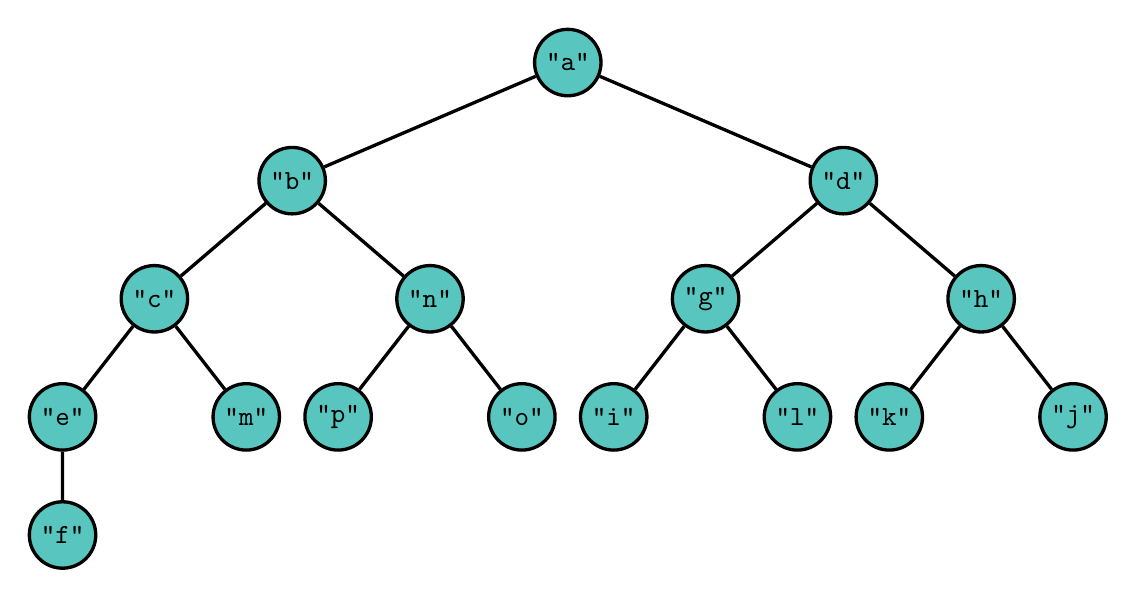
\begin{tikzpicture}[very thick,level/.style={sibling distance=70mm/#1}]
\node [vertex] (r){\texttt{"a"}}
  child {
    node [vertex] (a) {\texttt{"b"}}
    child {
      node [vertex] {\texttt{"c"}}
      child {
        node [vertex] {\texttt{"e"}}
        child {node [vertex] {\texttt{"f"}}}
      } 
      child {
        node [vertex] {\texttt{"m"}}
      }
    }
    child {
      node [vertex] {\texttt{"n"}}
      child {node [vertex] {\texttt{"p"}}}
      child {node [vertex] {\texttt{"o"}}}
    }
  }
  child {
    node [vertex] {\texttt{"d"}}
    child {
      node [vertex] {\texttt{"g"}}
      child {node [vertex] {\texttt{"i"}}}
      child {node [vertex] {\texttt{"l"}}}
    }
    child {
      node [vertex] {\texttt{"h"}}
      child {node [vertex] {\texttt{"k"}}}
      child {node [vertex] {\texttt{"j"}}}
    }
  };
\end{tikzpicture}
\end{center}

We see that the root of the tree will always be the top element. It is tempting to use a container class with a pointer to its left and its right child. However, we have a much nicer way to store \textit{complete} binary trees with an array. Consider the following numbering of the nodes:

\begin{center}
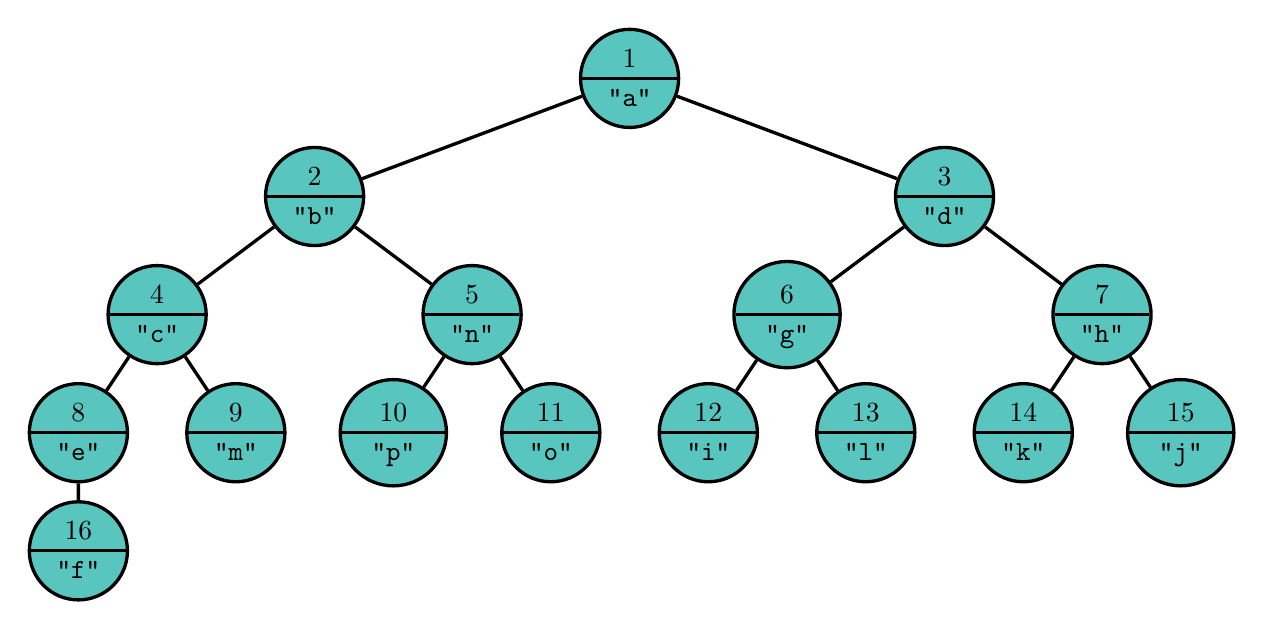
\begin{tikzpicture}[very thick,level 1/.style={sibling distance=80mm}, level 2/.style={sibling distance=40mm}, level 3/.style={sibling distance=20mm}]
\node [splitvertex] (r){1\nodepart{lower}\texttt{"a"}}
  child {
    node [splitvertex] (a) {2\nodepart{lower}\texttt{"b"}}
    child {
      node [splitvertex] {4\nodepart{lower}\texttt{"c"}}
      child {
        node [splitvertex] {8\nodepart{lower}\texttt{"e"}}
        child {node [splitvertex] {16\nodepart{lower}\texttt{"f"}}}
      } 
      child {
        node [splitvertex] {9\nodepart{lower}\texttt{"m"}}
      }
    }
    child {
      node [splitvertex] {5\nodepart{lower}\texttt{"n"}}
      child {node [splitvertex] {10\nodepart{lower}\texttt{"p"}}}
      child {node [splitvertex] {11\nodepart{lower}\texttt{"o"}}}
    }
  }
  child {
    node [splitvertex] {3\nodepart{lower}\texttt{"d"}}
    child {
      node [splitvertex] {6\nodepart{lower}\texttt{"g"}}
      child {node [splitvertex] {12\nodepart{lower}\texttt{"i"}}}
      child {node [splitvertex] {13\nodepart{lower}\texttt{"l"}}}
    }
    child {
      node [splitvertex] {7\nodepart{lower}\texttt{"h"}}
      child {node [splitvertex] {14\nodepart{lower}\texttt{"k"}}}
      child {node [splitvertex] {15\nodepart{lower}\texttt{"j"}}}
    }
  };
\end{tikzpicture}
\end{center}

We see that every number from 1 to 16 is used, and for every node, if the index associated with it is $i$, the left child is $2i$, and the right child is $2i+1$. This leads to a very natural implementation of the tree in an array:

\begin{center}
{
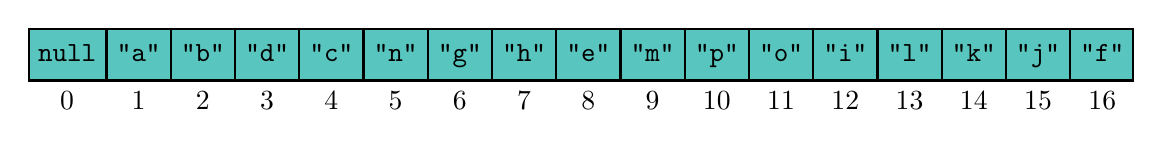
\begin{tikzpicture}[
  thick,
  myrect/.style={
    draw,
    fill=myseagreen,
    rectangle split,
    rectangle split horizontal,
    rectangle split parts=#1,
    rectangle split part align=left,
    text centered
    },
  mycallout/.style={
    shape=rectangle callout,
    rounded corners,
    fill=mysalmon,
    callout absolute pointer={#1},
    callout pointer width=1cm
  }  
]

\node[myrect=17]
  (array)
  {
  					\strut \texttt{null}
  \nodepart{two}	\strut \texttt{"a"}
  \nodepart{three}	\strut \texttt{"b"}
  \nodepart{four}	\strut \texttt{"d"}
  \nodepart{five}	\strut \texttt{"c"}
  \nodepart{six}	\strut \texttt{"n"}
  \nodepart{seven}	\strut \texttt{"g"}
  \nodepart{eight}	\strut \texttt{"h"}
  \nodepart{nine}	\strut \texttt{"e"}
  \nodepart{ten}	\strut \texttt{"m"}
  \nodepart{eleven}	\strut \texttt{"p"}
  \nodepart{twelve}	\strut \texttt{"o"}
  \nodepart{thirteen}	\strut \texttt{"i"}
  \nodepart{fourteen}	\strut \texttt{"l"}
  \nodepart{fifteen}	\strut \texttt{"k"}
  \nodepart{sixteen}	\strut \texttt{"j"}
  \nodepart{seventeen}	\strut \texttt{"f"}
  };
\foreach \Valor [count=\Valori from 0] in {one ,two ,three ,four ,five ,six ,seven ,eight ,nine ,ten ,eleven ,twelve ,thirteen ,fourteen ,fifteen ,sixteen ,seventeen }
  \node[below] at (array.\Valor south) {\Valori};

\end{tikzpicture}
}
\end{center}

How do we add elements to our heap, while maintaining the heap qualities? Well, let's just add it to the very end and see what we get. Suppose we are to add \texttt{"b"} to the tree.

\begin{center}
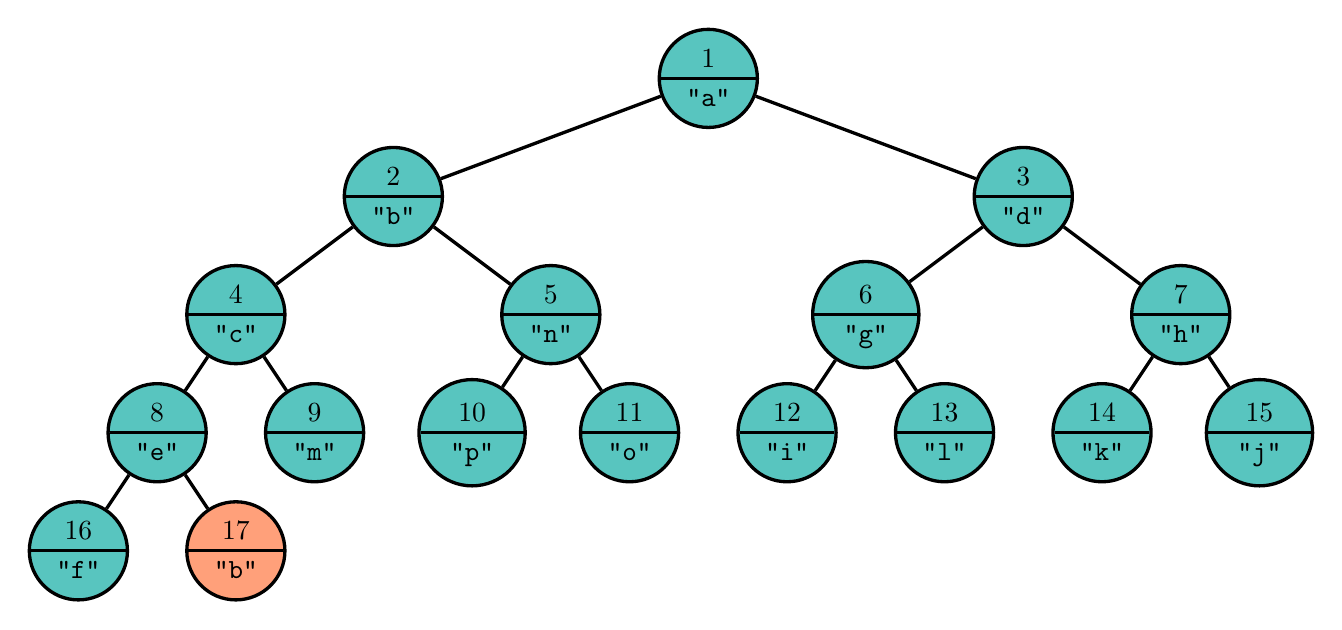
\begin{tikzpicture}[very thick,level 1/.style={sibling distance=80mm}, level 2/.style={sibling distance=40mm}, level 3/.style={sibling distance=20mm}]
\node [splitvertex] (r){1\nodepart{lower}\texttt{"a"}}
  child {
    node [splitvertex] (a) {2\nodepart{lower}\texttt{"b"}}
    child {
      node [splitvertex] {4\nodepart{lower}\texttt{"c"}}
      child {
        node [splitvertex] {8\nodepart{lower}\texttt{"e"}}
        child {node [splitvertex] {16\nodepart{lower}\texttt{"f"}}}
        child {node [splitvertex, fill=mysalmon] {17\nodepart{lower}\texttt{"b"}}}
      } 
      child {
        node [splitvertex] {9\nodepart{lower}\texttt{"m"}}
      }
    }
    child {
      node [splitvertex] {5\nodepart{lower}\texttt{"n"}}
      child {node [splitvertex] {10\nodepart{lower}\texttt{"p"}}}
      child {node [splitvertex] {11\nodepart{lower}\texttt{"o"}}}
    }
  }
  child {
    node [splitvertex] {3\nodepart{lower}\texttt{"d"}}
    child {
      node [splitvertex] {6\nodepart{lower}\texttt{"g"}}
      child {node [splitvertex] {12\nodepart{lower}\texttt{"i"}}}
      child {node [splitvertex] {13\nodepart{lower}\texttt{"l"}}}
    }
    child {
      node [splitvertex] {7\nodepart{lower}\texttt{"h"}}
      child {node [splitvertex] {14\nodepart{lower}\texttt{"k"}}}
      child {node [splitvertex] {15\nodepart{lower}\texttt{"j"}}}
    }
  };
\end{tikzpicture}
\end{center}

Well, \texttt{"b"} comes before \texttt{"e"} in the alphabet, so let's swap the nodes. We are guaranteed that \texttt{"b"} should come before the other child (in this case, \texttt{"f"}) by the transitive property.

\begin{center}
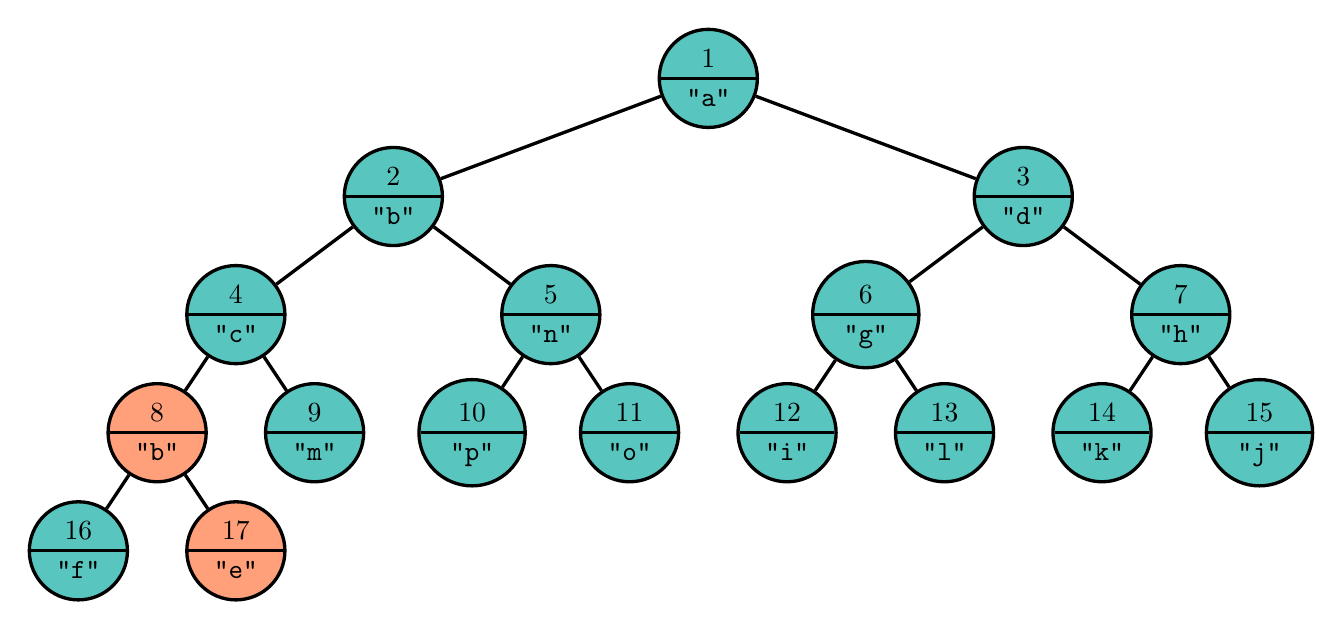
\begin{tikzpicture}[very thick,level 1/.style={sibling distance=80mm}, level 2/.style={sibling distance=40mm}, level 3/.style={sibling distance=20mm}]
\node [splitvertex] (r){1\nodepart{lower}\texttt{"a"}}
  child {
    node [splitvertex] (a) {2\nodepart{lower}\texttt{"b"}}
    child {
      node [splitvertex] {4\nodepart{lower}\texttt{"c"}}
      child {
        node [splitvertex, fill=mysalmon] {8\nodepart{lower}\texttt{"b"}}
        child {node [splitvertex] {16\nodepart{lower}\texttt{"f"}}}
        child {node [splitvertex, fill=mysalmon] {17\nodepart{lower}\texttt{"e"}}}
      } 
      child {
        node [splitvertex] {9\nodepart{lower}\texttt{"m"}}
      }
    }
    child {
      node [splitvertex] {5\nodepart{lower}\texttt{"n"}}
      child {node [splitvertex] {10\nodepart{lower}\texttt{"p"}}}
      child {node [splitvertex] {11\nodepart{lower}\texttt{"o"}}}
    }
  }
  child {
    node [splitvertex] {3\nodepart{lower}\texttt{"d"}}
    child {
      node [splitvertex] {6\nodepart{lower}\texttt{"g"}}
      child {node [splitvertex] {12\nodepart{lower}\texttt{"i"}}}
      child {node [splitvertex] {13\nodepart{lower}\texttt{"l"}}}
    }
    child {
      node [splitvertex] {7\nodepart{lower}\texttt{"h"}}
      child {node [splitvertex] {14\nodepart{lower}\texttt{"k"}}}
      child {node [splitvertex] {15\nodepart{lower}\texttt{"j"}}}
    }
  };
\end{tikzpicture}
\end{center}

One more swap...

\begin{center}
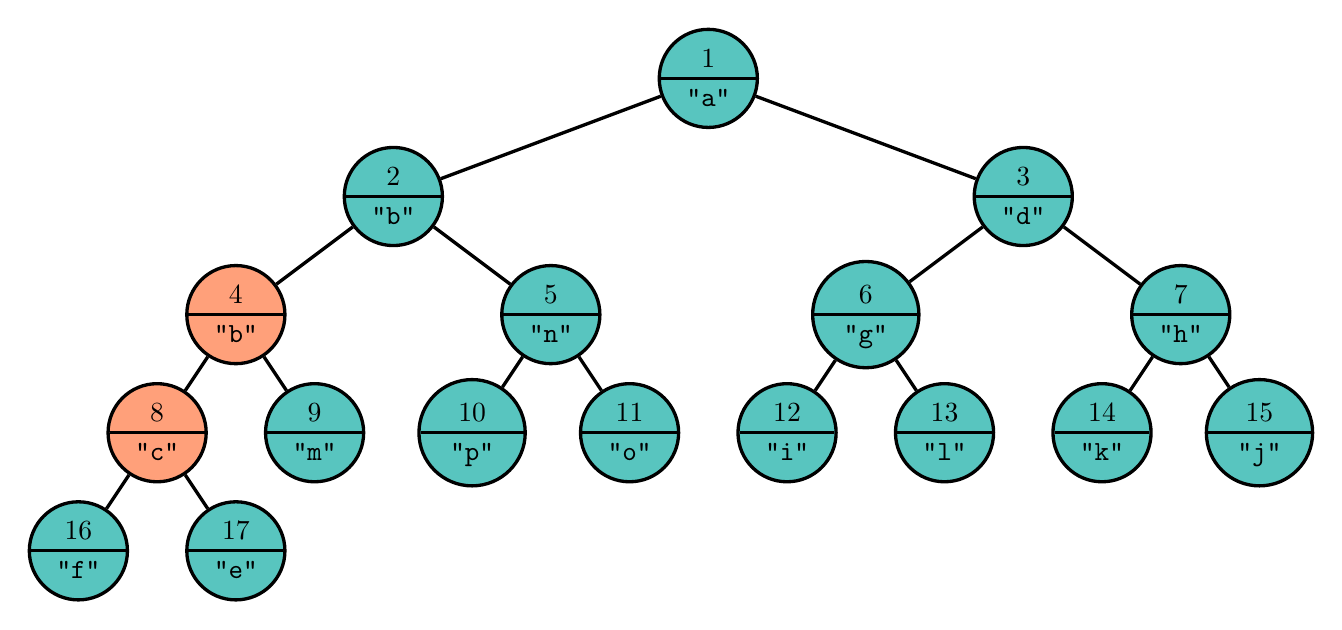
\begin{tikzpicture}[very thick,level 1/.style={sibling distance=80mm}, level 2/.style={sibling distance=40mm}, level 3/.style={sibling distance=20mm}]
\node [splitvertex] (r){1\nodepart{lower}\texttt{"a"}}
  child {
    node [splitvertex] (a) {2\nodepart{lower}\texttt{"b"}}
    child {
      node [splitvertex, fill=mysalmon] {4\nodepart{lower}\texttt{"b"}}
      child {
        node [splitvertex, fill=mysalmon] {8\nodepart{lower}\texttt{"c"}}
        child {node [splitvertex] {16\nodepart{lower}\texttt{"f"}}}
        child {node [splitvertex] {17\nodepart{lower}\texttt{"e"}}}
      } 
      child {
        node [splitvertex] {9\nodepart{lower}\texttt{"m"}}
      }
    }
    child {
      node [splitvertex] {5\nodepart{lower}\texttt{"n"}}
      child {node [splitvertex] {10\nodepart{lower}\texttt{"p"}}}
      child {node [splitvertex] {11\nodepart{lower}\texttt{"o"}}}
    }
  }
  child {
    node [splitvertex] {3\nodepart{lower}\texttt{"d"}}
    child {
      node [splitvertex] {6\nodepart{lower}\texttt{"g"}}
      child {node [splitvertex] {12\nodepart{lower}\texttt{"i"}}}
      child {node [splitvertex] {13\nodepart{lower}\texttt{"l"}}}
    }
    child {
      node [splitvertex] {7\nodepart{lower}\texttt{"h"}}
      child {node [splitvertex] {14\nodepart{lower}\texttt{"k"}}}
      child {node [splitvertex] {15\nodepart{lower}\texttt{"j"}}}
    }
  };
\end{tikzpicture}
\end{center}

And now we have the heap property restored. As the tree has depth at most $\log{n}$, this process is $O(\log{n})$.

To remove the root from the heap, we replace the root with the last leaf:

\begin{center}
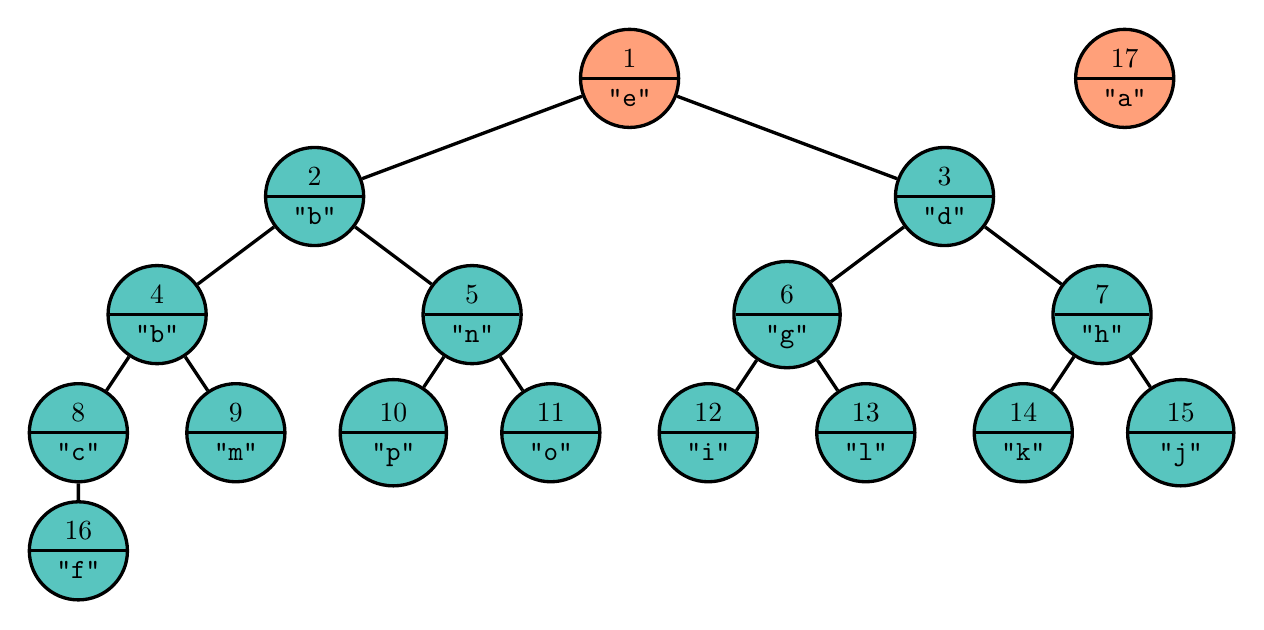
\begin{tikzpicture}[very thick,level 1/.style={sibling distance=80mm}, level 2/.style={sibling distance=40mm}, level 3/.style={sibling distance=20mm}]
\node [splitvertex, fill=mysalmon] (r){1\nodepart{lower}\texttt{"e"}}
  child {
    node [splitvertex] (a) {2\nodepart{lower}\texttt{"b"}}
    child {
      node [splitvertex] {4\nodepart{lower}\texttt{"b"}}
      child {
        node [splitvertex] {8\nodepart{lower}\texttt{"c"}}
        child {node [splitvertex] {16\nodepart{lower}\texttt{"f"}}}
      } 
      child {
        node [splitvertex] {9\nodepart{lower}\texttt{"m"}}
      }
    }
    child {
      node [splitvertex] {5\nodepart{lower}\texttt{"n"}}
      child {node [splitvertex] {10\nodepart{lower}\texttt{"p"}}}
      child {node [splitvertex] {11\nodepart{lower}\texttt{"o"}}}
    }
  }
  child {
    node [splitvertex] {3\nodepart{lower}\texttt{"d"}}
    child {
      node [splitvertex] {6\nodepart{lower}\texttt{"g"}}
      child {node [splitvertex] {12\nodepart{lower}\texttt{"i"}}}
      child {node [splitvertex] {13\nodepart{lower}\texttt{"l"}}}
    }
    child {
      node [splitvertex] {7\nodepart{lower}\texttt{"h"}}
      child {node [splitvertex] {14\nodepart{lower}\texttt{"k"}}}
      child {node [splitvertex] {15\nodepart{lower}\texttt{"j"}}}
    }
  };
  \node [splitvertex, fill=mysalmon] [right=5cm of r]{17\nodepart{lower}\texttt{"a"}};
\end{tikzpicture}
\end{center}

We perform a series of swaps to restore the heap property. We always want to choose the smaller child to swap until the heap property is satisfied.

\begin{center}
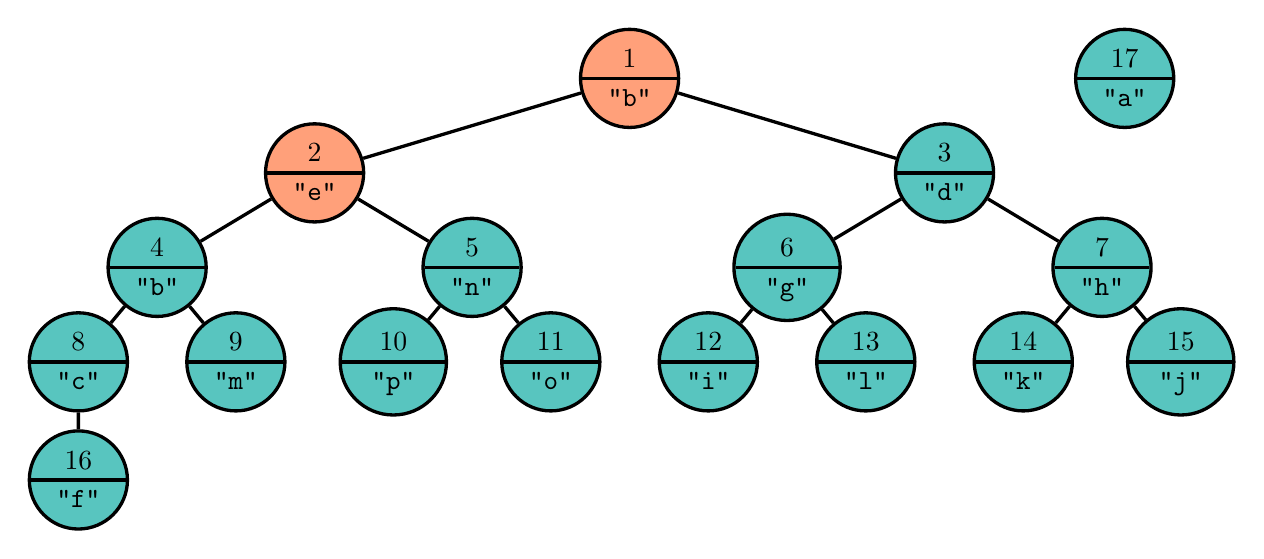
\begin{tikzpicture}[very thick,level 1/.style={sibling distance=80mm}, level 2/.style={sibling distance=40mm}, level 3/.style={sibling distance=20mm}, level distance=12mm, level 4/.style={level distance=15mm}]
\node [splitvertex, fill=mysalmon] (r){1\nodepart{lower}\texttt{"b"}}
  child {
    node [splitvertex, fill=mysalmon] (a) {2\nodepart{lower}\texttt{"e"}}
    child {
      node [splitvertex] {4\nodepart{lower}\texttt{"b"}}
      child {
        node [splitvertex] {8\nodepart{lower}\texttt{"c"}}
        child {node [splitvertex] {16\nodepart{lower}\texttt{"f"}}}
      } 
      child {
        node [splitvertex] {9\nodepart{lower}\texttt{"m"}}
      }
    }
    child {
      node [splitvertex] {5\nodepart{lower}\texttt{"n"}}
      child {node [splitvertex] {10\nodepart{lower}\texttt{"p"}}}
      child {node [splitvertex] {11\nodepart{lower}\texttt{"o"}}}
    }
  }
  child {
    node [splitvertex] {3\nodepart{lower}\texttt{"d"}}
    child {
      node [splitvertex] {6\nodepart{lower}\texttt{"g"}}
      child {node [splitvertex] {12\nodepart{lower}\texttt{"i"}}}
      child {node [splitvertex] {13\nodepart{lower}\texttt{"l"}}}
    }
    child {
      node [splitvertex] {7\nodepart{lower}\texttt{"h"}}
      child {node [splitvertex] {14\nodepart{lower}\texttt{"k"}}}
      child {node [splitvertex] {15\nodepart{lower}\texttt{"j"}}}
    }
  };
  \node [splitvertex] [right=5cm of r]{17\nodepart{lower}\texttt{"a"}};
\end{tikzpicture}
\end{center}

\begin{center}
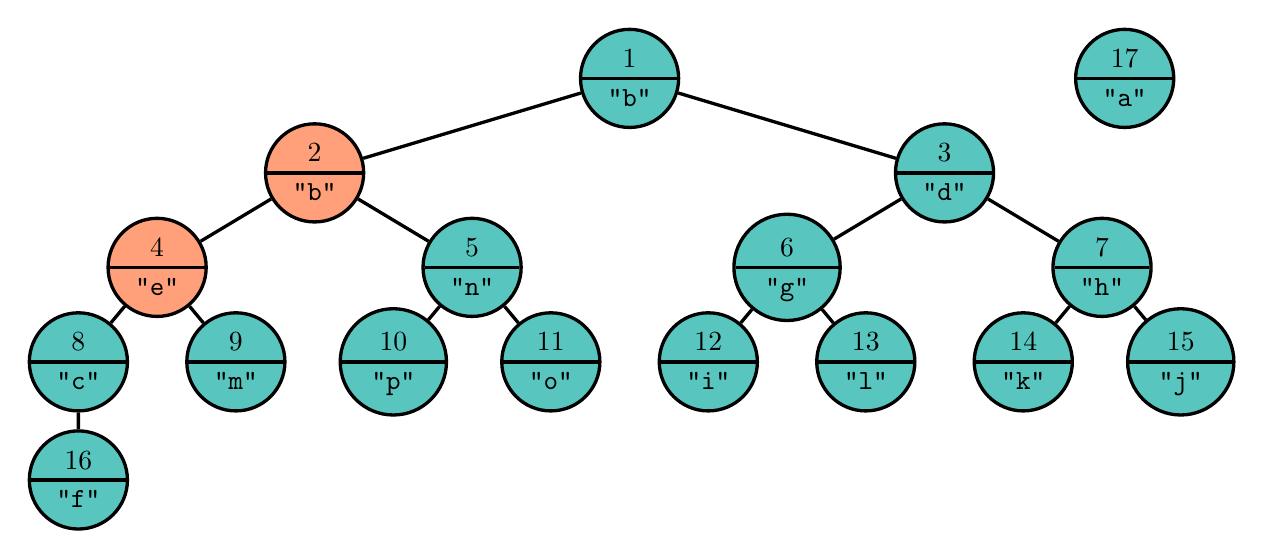
\begin{tikzpicture}[very thick,level 1/.style={sibling distance=80mm}, level 2/.style={sibling distance=40mm}, level 3/.style={sibling distance=20mm}, level distance=12mm, level 4/.style={level distance=15mm}]
\node [splitvertex] (r){1\nodepart{lower}\texttt{"b"}}
  child {
    node [splitvertex, fill=mysalmon] (a) {2\nodepart{lower}\texttt{"b"}}
    child {
      node [splitvertex, fill=mysalmon] {4\nodepart{lower}\texttt{"e"}}
      child {
        node [splitvertex] {8\nodepart{lower}\texttt{"c"}}
        child {node [splitvertex] {16\nodepart{lower}\texttt{"f"}}}
      } 
      child {
        node [splitvertex] {9\nodepart{lower}\texttt{"m"}}
      }
    }
    child {
      node [splitvertex] {5\nodepart{lower}\texttt{"n"}}
      child {node [splitvertex] {10\nodepart{lower}\texttt{"p"}}}
      child {node [splitvertex] {11\nodepart{lower}\texttt{"o"}}}
    }
  }
  child {
    node [splitvertex] {3\nodepart{lower}\texttt{"d"}}
    child {
      node [splitvertex] {6\nodepart{lower}\texttt{"g"}}
      child {node [splitvertex] {12\nodepart{lower}\texttt{"i"}}}
      child {node [splitvertex] {13\nodepart{lower}\texttt{"l"}}}
    }
    child {
      node [splitvertex] {7\nodepart{lower}\texttt{"h"}}
      child {node [splitvertex] {14\nodepart{lower}\texttt{"k"}}}
      child {node [splitvertex] {15\nodepart{lower}\texttt{"j"}}}
    }
  };
  \node [splitvertex] [right=5cm of r]{17\nodepart{lower}\texttt{"a"}};
\end{tikzpicture}
\end{center}

\begin{center}
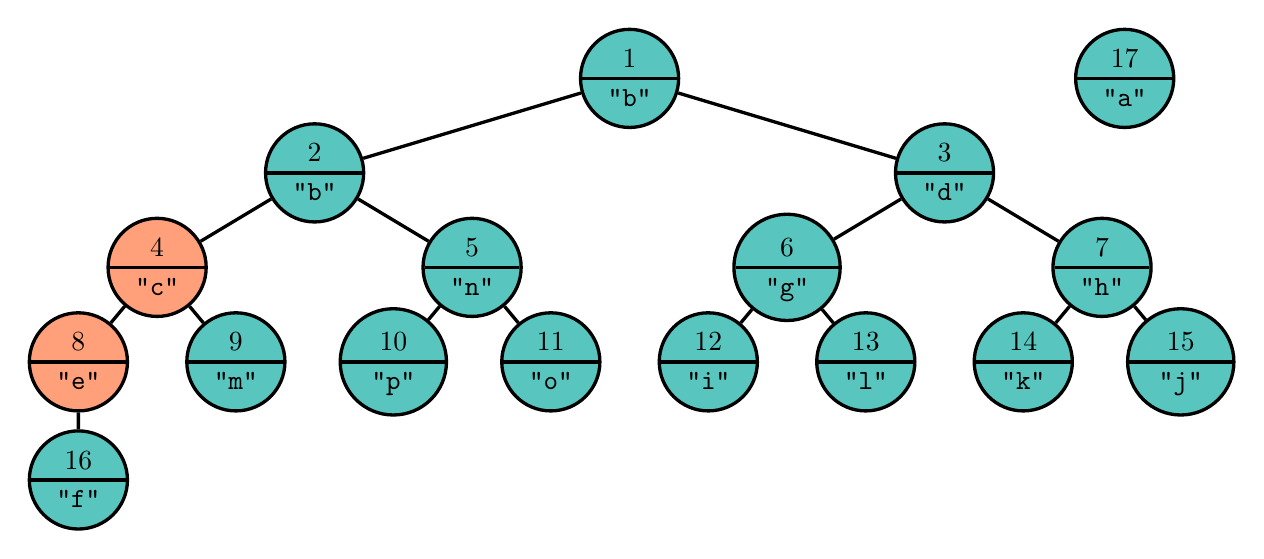
\begin{tikzpicture}[very thick,level 1/.style={sibling distance=80mm}, level 2/.style={sibling distance=40mm}, level 3/.style={sibling distance=20mm}, level distance=12mm, level 4/.style={level distance=15mm}]
\node [splitvertex] (r){1\nodepart{lower}\texttt{"b"}}
  child {
    node [splitvertex] (a) {2\nodepart{lower}\texttt{"b"}}
    child {
      node [splitvertex, fill=mysalmon] {4\nodepart{lower}\texttt{"c"}}
      child {
        node [splitvertex, fill=mysalmon] {8\nodepart{lower}\texttt{"e"}}
        child {node [splitvertex] {16\nodepart{lower}\texttt{"f"}}}
      } 
      child {
        node [splitvertex] {9\nodepart{lower}\texttt{"m"}}
      }
    }
    child {
      node [splitvertex] {5\nodepart{lower}\texttt{"n"}}
      child {node [splitvertex] {10\nodepart{lower}\texttt{"p"}}}
      child {node [splitvertex] {11\nodepart{lower}\texttt{"o"}}}
    }
  }
  child {
    node [splitvertex] {3\nodepart{lower}\texttt{"d"}}
    child {
      node [splitvertex] {6\nodepart{lower}\texttt{"g"}}
      child {node [splitvertex] {12\nodepart{lower}\texttt{"i"}}}
      child {node [splitvertex] {13\nodepart{lower}\texttt{"l"}}}
    }
    child {
      node [splitvertex] {7\nodepart{lower}\texttt{"h"}}
      child {node [splitvertex] {14\nodepart{lower}\texttt{"k"}}}
      child {node [splitvertex] {15\nodepart{lower}\texttt{"j"}}}
    }
  };
  \node [splitvertex] [right=5cm of r]{17\nodepart{lower}\texttt{"a"}};
\end{tikzpicture}
\end{center}

And we are done. Once again, this takes at most $\log(N)$ swaps. This idea can be extended to removing or changing the value of any node we'd like from a tree -- this is particularly useful for Dijkstra later.

Remember to implement your heap in an array or ArrayList!

\begin{itemize}

\item \texttt{boolean add(String s)}

\item \texttt{boolean isEmpty()}

\item \texttt{String poll()}

\item \texttt{String peek()}

\item \texttt{int size()}

\end{itemize}

\section{Set}

A Set is a collection of objects with no duplicate elements. Set is a Java interface. Note that the data structures discussed in this section can be extended to become multisets, but Java implementations of these explicitly disallow multiplicity.

\subsection{TreeSet}

A TreeSet is Java's implementation of a \textit{binary search tree} (BST). A binary search tree is a tree where every node is greater than every node in its left subtree and less than every node in its right subtree. As with a heap, to use a BST, we need to impose some kind of ordering on the elements stored.

\begin{center}
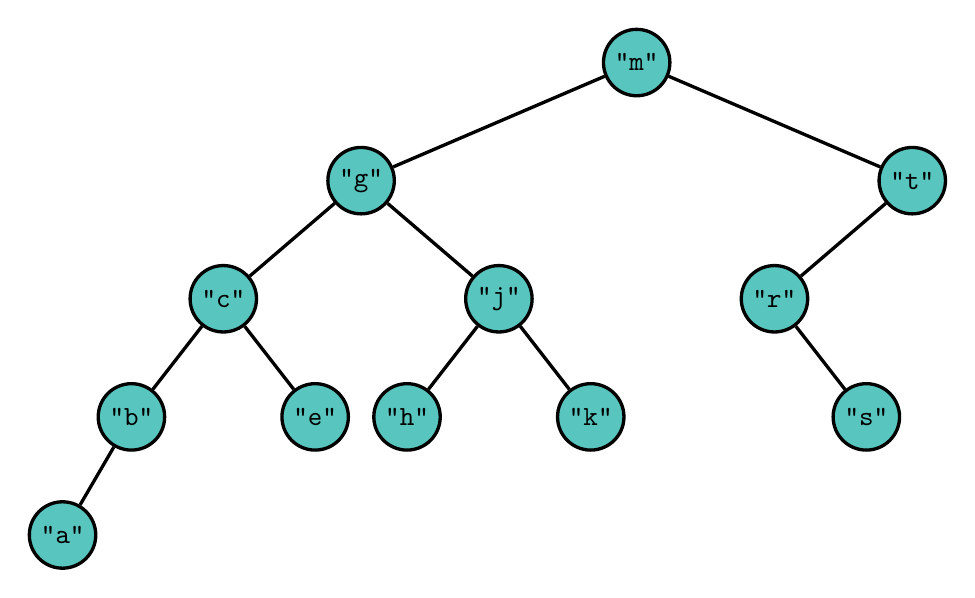
\begin{tikzpicture}[very thick,level/.style={sibling distance=70mm/#1}]
\node [vertex] (r){\texttt{"m"}}
  child {
    node [vertex] {\texttt{"g"}}
    child {
      node [vertex] {\texttt{"c"}}
      child {
        node [vertex] {\texttt{"b"}}
        child {node [vertex] {\texttt{"a"}}}
        child[missing]
      } 
      child {
        node [vertex] {\texttt{"e"}}
      }
    }
    child {
      node [vertex] {\texttt{"j"}}
      child {node [vertex] {\texttt{"h"}}}
      child {node [vertex] {\texttt{"k"}}}
    }
  }
  child {
    node [vertex] {\texttt{"t"}}
    child {
      node [vertex] {\texttt{"r"}}
      child[missing]
      child {node [vertex] {\texttt{"s"}}}
    }
    child[missing]
  };
\end{tikzpicture}
\end{center}

The tree need not be complete. Because it is not complete, there is no way to nicely bound the size of the array we would need if we were to use the same storage method as with the heap. Thus, we are forced to use a TreeNode, with left and right pointers. This is also problematic when determining guarantees on time complexities later, but the ways to solve this problem are pretty complicated so we'll ignore them for now.

Given the name of the tree, searching for an element within the tree is quite natural, and similar to a binary search. Compare the element to be searched for with the current node. If they are equal, we are done; otherwise, search the appropriate left or right subtree. As with most structures and algorithms with a binary search structure, this operation lends itself nicely to recursion. If the tree is reasonably nice, we expect to complete this in $O(\log{n})$ time, but searching can be as bad as linear if the tree looks like a LinkedList.

Adding an element is also natural. As our tree represents a set, it will not contain the same element twice. We trace down until we hit a null pointer, and add the element in the appropriate spot. Let's add a \texttt{"p"} to the BST:

\begin{center}
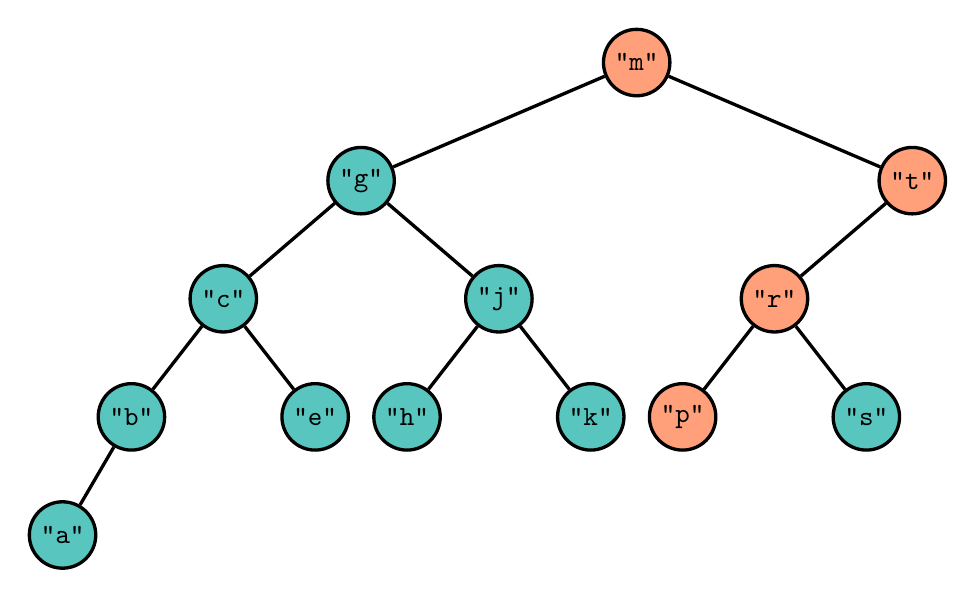
\begin{tikzpicture}[very thick,level/.style={sibling distance=70mm/#1}]
\node [vertex, fill=mysalmon] (r){\texttt{"m"}}
  child {
    node [vertex] {\texttt{"g"}}
    child {
      node [vertex] {\texttt{"c"}}
      child {
        node [vertex] {\texttt{"b"}}
        child {node [vertex] {\texttt{"a"}}}
        child[missing]
      } 
      child {
        node [vertex] {\texttt{"e"}}
      }
    }
    child {
      node [vertex] {\texttt{"j"}}
      child {node [vertex] {\texttt{"h"}}}
      child {node [vertex] {\texttt{"k"}}}
    }
  }
  child {
    node [vertex, fill=mysalmon] {\texttt{"t"}}
    child {
      node [vertex, fill=mysalmon] {\texttt{"r"}}
      child {node [vertex, fill=mysalmon] {\texttt{"p"}}}
      child {node [vertex] {\texttt{"s"}}}
    }
    child[missing]
  };
\end{tikzpicture}
\end{center}

Deleting an element is the annoying part. Unfortunately, there's not much we can do besides casework.

Removing a leaf, like \texttt{"a"}, from the tree is very easy. Removing a node with only once child, like \texttt{"t"}, is also relatively straightforward.

\begin{center}
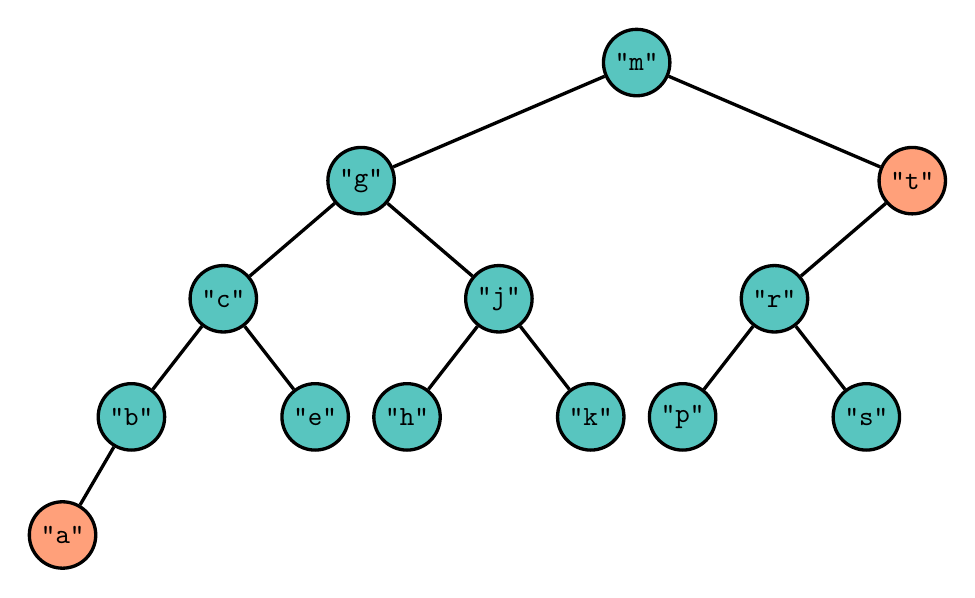
\begin{tikzpicture}[very thick,level/.style={sibling distance=70mm/#1}]
\node [vertex] (r){\texttt{"m"}}
  child {
    node [vertex] {\texttt{"g"}}
    child {
      node [vertex] {\texttt{"c"}}
      child {
        node [vertex] {\texttt{"b"}}
        child {node [vertex,fill=mysalmon] {\texttt{"a"}}}
        child[missing]
      } 
      child {
        node [vertex] {\texttt{"e"}}
      }
    }
    child {
      node [vertex] {\texttt{"j"}}
      child {node [vertex] {\texttt{"h"}}}
      child {node [vertex] {\texttt{"k"}}}
    }
  }
  child {
    node [vertex, fill=mysalmon] {\texttt{"t"}}
    child {
      node [vertex] {\texttt{"r"}}
      child {node [vertex] {\texttt{"p"}}}
      child {node [vertex] {\texttt{"s"}}}
    }
    child[missing]
  };
\end{tikzpicture}
\end{center}

Now, removing an element with two children is tricky. We'll try to remove \texttt{"g"}. Consider the least element in the right subtree of \texttt{"g"}, which in this case is \texttt{"h"}. We find \texttt{"h"} by always choosing the left child on the right subtree until we cannot go any further. This must be the least element.

\begin{center}
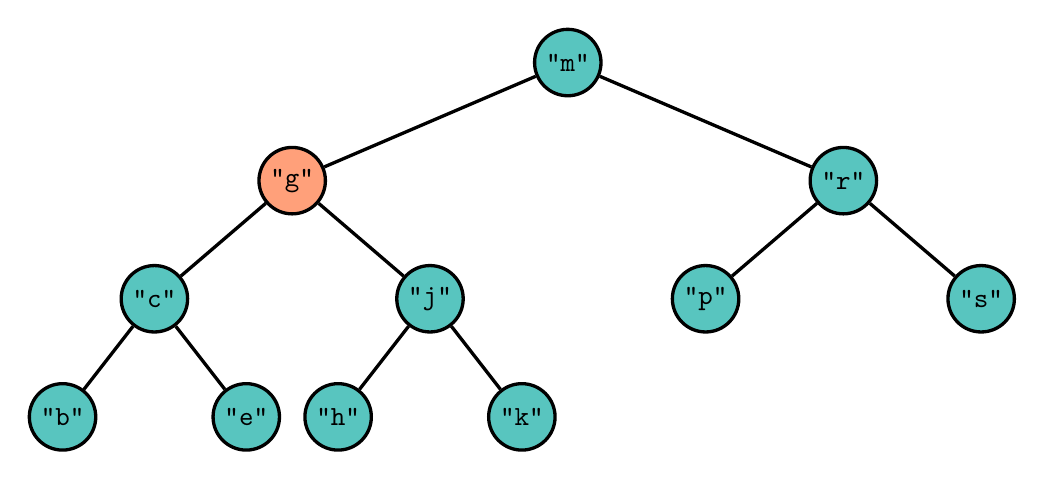
\begin{tikzpicture}[very thick,level/.style={sibling distance=70mm/#1}]
\node [vertex] (r){\texttt{"m"}}
  child {
    node [vertex, fill=mysalmon] {\texttt{"g"}}
    child {
      node [vertex] {\texttt{"c"}}
      child {
        node [vertex] {\texttt{"b"}}
      } 
      child {
        node [vertex] {\texttt{"e"}}
      }
    }
    child {
      node [vertex] {\texttt{"j"}}
      child {node [vertex] {\texttt{"h"}}}
      child {node [vertex] {\texttt{"k"}}}
    }
  }
  child {
      node [vertex] {\texttt{"r"}}
      child {node [vertex] {\texttt{"p"}}}
      child {node [vertex] {\texttt{"s"}}}
  };
\end{tikzpicture}
\end{center}

Note that \texttt{"h"} has either no children or only one child, and that nodes like these are easy to remove. We then change the value of the node containing \texttt{"g"} to \texttt{"h"}, which is legal since \texttt{"h"} is the least element, and remove \texttt{"h"} from the right subtree, and we are done.

\begin{center}
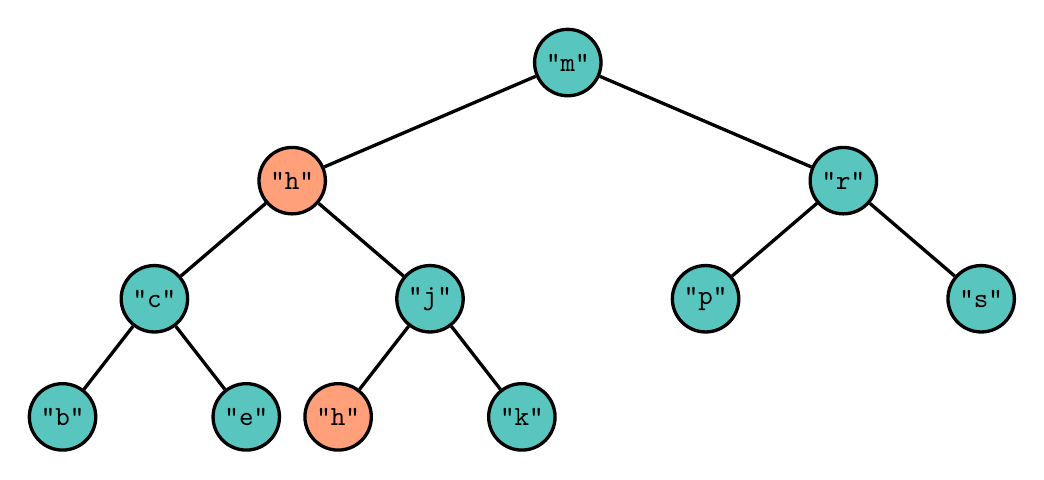
\begin{tikzpicture}[very thick,level/.style={sibling distance=70mm/#1}]
\node [vertex] (r){\texttt{"m"}}
  child {
    node [vertex, fill=mysalmon] {\texttt{"h"}}
    child {
      node [vertex] {\texttt{"c"}}
      child {
        node [vertex] {\texttt{"b"}}
      } 
      child {
        node [vertex] {\texttt{"e"}}
      }
    }
    child {
      node [vertex] {\texttt{"j"}}
      child {node [vertex, fill=mysalmon] {\texttt{"h"}}}
      child {node [vertex] {\texttt{"k"}}}
    }
  }
  child {
      node [vertex] {\texttt{"r"}}
      child {node [vertex] {\texttt{"p"}}}
      child {node [vertex] {\texttt{"s"}}}
  };
\end{tikzpicture}
\end{center}

\begin{center}
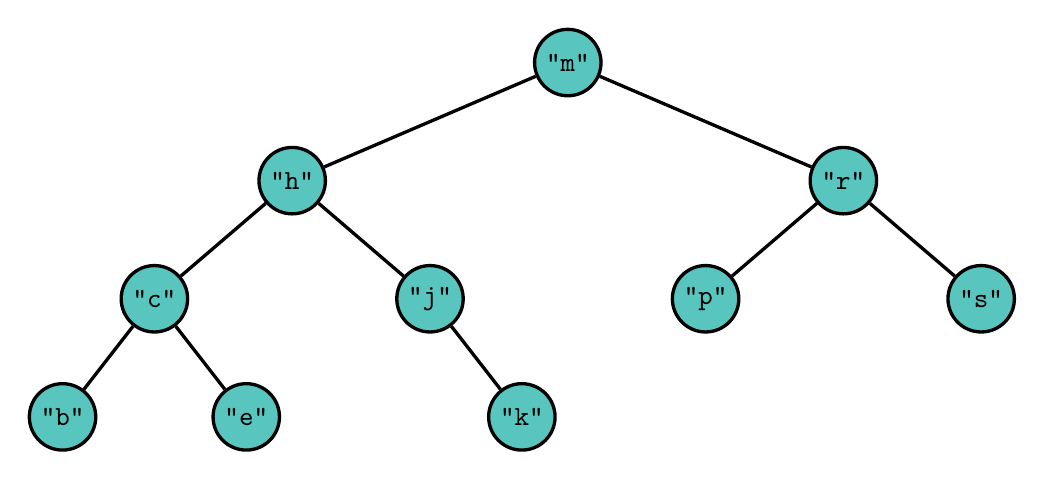
\begin{tikzpicture}[very thick,level/.style={sibling distance=70mm/#1}]
\node [vertex] (r){\texttt{"m"}}
  child {
    node [vertex] {\texttt{"h"}}
    child {
      node [vertex] {\texttt{"c"}}
      child {
        node [vertex] {\texttt{"b"}}
      } 
      child {
        node [vertex] {\texttt{"e"}}
      }
    }
      child {node [vertex] {\texttt{"j"}}
      	child[missing]
        child {
        	node[vertex]{\texttt{"k"}}
        }
      }
  }
  child {
      node [vertex] {\texttt{"r"}}
      child {node [vertex] {\texttt{"p"}}}
      child {node [vertex] {\texttt{"s"}}}
  };
\end{tikzpicture}
\end{center}

A standard BST has $O(\log{n})$ operations if the tree is ``nice'', but each operation can be $O(n)$ in the worst case. We need to find a way to automatically balance the BST such that we avoid linear time complexities.

A red-black tree is a self-balancing BST that guarantees $O(\log{n})$ operations by making sure the height of the tree grows logarithmically. It is implemented in Java's TreeSet, so while the BST I described above does not guarantee nice time bounds, Java's implementation does.

I don't think learning exactly how a red-black tree works is particularly useful for the beginning programmer. How exactly a red-black tree works, together with some more balanced binary search trees which are useful on the competitive scene, are covered in a later chapter.

Here are some notable functions TreeSet implements. You don't need to implement everything -- \texttt{add()}, \texttt{remove()}, and \texttt{contains()} are the most important.

\begin{itemize}

\item
\texttt{boolean add(String s)}

\item
\texttt{String ceiling(String s)} -- the least element in the set greater than or equal to \texttt{s}, or \texttt{null} if there is no such element.

\item
\texttt{boolean contains(Object o)}

\item
\texttt{String first()} -- the least element in the set.

\item
\texttt{String floor(String s)} -- the greatest element in the set less than or equal to \texttt{s}, or \texttt{null} if there is no such element.

\item
\texttt{String higher(String s)} -- the least element in the set strictly greater than \texttt{s}, or \texttt{null} if there is no such element.

\item
\texttt{boolean isEmpty()}

\item
\texttt{String last()} -- the greatest element in the set.

\item
\texttt{String lower(String s)} -- the greatest element in the set strictly less than \texttt{s}, or \texttt{null} if there is no such element.

\item
\texttt{boolean remove(Object o)}

\item
\texttt{int size()}

\end{itemize}

Since the TreeSet is ordered, iterating over a TreeSet will also be in order.

\subsection{HashSet}

A HashSet is a way for us to store objects when we do not require a natural ordering on the set. As with the TreeSet, we want to be able to check whether an element is in our set or not quickly. We do this with the help of a \textit{hash function}. Every Java Object supports the \texttt{hashCode()} function. We usually want to map an object with an integer hash, so that we can store the values in an array. For example, let us define the following hash for Strings:

\begin{mylstlisting}
public int hashCode() {
	int hash = 0;
    for(int k = 0; k < length(); k++) {
		hash *= 31;
        hash += (int) (charAt(k));
    }
    return hash;
}
\end{mylstlisting}

\texttt{a.equals(b)} should imply \texttt{a.hashCode() == b.hashCode()}. This function produces the same result as the actual \texttt{hashCode()} function in the String class. However, this is not quite what we want for our HashSet, because in the end we wish to be able to store the objects in some kind of array. This hash not only returns integers that can be very large, they can also be negative, and thus are not suitable as array indices. The natural way to fix this is to take the hash modulo the size of the array we want.

\begin{mylstlisting}
String[] table = new String[10007];
int index(String s) {
	int i = s.hashCode() % table.length;
    if(i >= 0)
    	return i;
	return i + table.length;
}
\end{mylstlisting}

We chose the number 10007 because it is a prime number, and primes are generally nice when taking a number modulo something else, as integers modulo a prime form a field. Remember that a negative number \texttt{\%} another number is not necessarily positive, so we need to be a little careful.

From here, adding an element to the HashSet and checking if an element is contained both seem straightforward:

\begin{mylstlisting}
boolean add (String s) {
	table[index(s)] = s;
    return true;
}
boolean contains(Object o) {
    int i = index((String) o);
	return table[i] != null && table[i].equals(o);
}
\end{mylstlisting}

\texttt{null} is always annoying to deal with, and will have to be handled separately.

However, one problem quickly arises. Two Strings may map to the same index in the array. We call this a \textit{collision}. The easiest way to handle a collision is by \textit{chaining}. We change the hash table to store a LinkedList instead of a single element in the event of a collision. Java once implemented this method of resolving collisions, but recently changed the LinkedList to a BST in Java 8.

\begin{itemize}

\item
\texttt{boolean add(String s)}

\item
\texttt{boolean contains(Object o)}

\item
\texttt{boolean isEmpty()}

\item
\texttt{boolean remove(Object o)}

\item
\texttt{int size()}

\end{itemize}

\section{Map}

A Map is simply an extension of a Set. It stores a mapping that takes a key to a value. Map is a Java Interface. Generics for Maps therefore have two arguments. Consider the following Map from Strings to Strings.

\begin{mylstlisting}
Map<String, String> email = new TreeMap<String, String>();
email.put("Samuel Hsiang", "samuel.c.hsiang@gmail.com");
\end{mylstlisting}

The keys of a Map form a Set, though the Values need not be unique.

The TreeMap is the Map variant of the TreeSet; similarly, the HashMap is the Map variant of the HashSet.

All useful Set functions have a Map counterpart. The following additional functions are of use.

\begin{itemize}

\item
\texttt{String get(Object k)} -- return the value assigned to \texttt{k}.

\item
\texttt{Set<String> keySet()} -- returns the set of keys.

\item
\texttt{Integer put(String k, String v)} -- assigns the value \texttt{k} to the key \texttt{v}, and returns the old value assigned to \texttt{k}.

\end{itemize}

\section{BigInteger}

BigInteger is in \texttt{java.math} for times when int and long just aren't large enough. The way BigInteger works is it stores a number as an array of ints. Each value in the array represents a digit in some very large base. Addition and subtraction can be done in the standard way. Generally multiplying two BigIntegers is not necessary on contests, but it can be sped up using Karatsuba or the FFT.

\section{C++ Analogs}

\begin{itemize}

\item \texttt{ArrayList} -- \texttt{vector}
\item \texttt{LinkedList} -- \texttt{list} or \texttt{deque}
\item \texttt{Stack} -- \texttt{stack}
\item \texttt{Queue} -- \texttt{queue}
\item \texttt{PriorityQueue} -- \texttt{priority\_queue}, but note that \texttt{priority\_queue} pops \textit{max} element first
\item \texttt{TreeSet} -- \texttt{set}
\item \texttt{HashSet} -- \texttt{unordered\_set}, C++11
\item \texttt{TreeMap} -- \texttt{map}
\item \texttt{HashMap} -- \texttt{unordered\_map}, C++11
\item \texttt{BigInteger} -- no equivalent

\end{itemize}


\chapter{Big Ideas}

In this chapter we'll discuss some general ideas for solving problems. These include brute force,  depth-first search, greedy algorithms, binary search, and dynamic programming. We can think of them as the building blocks of more complex algorithms---each provides a very general approach to simplifying problems. Since the concepts we cover are independent of language, the algorithms presented will no longer be in the form of concrete Java or C++ code but rather in more abstract pseudocode.

\section{Brute Force}

Sometimes, the best way to approach a problem is to try everything. This idea of exhaustively searching all possibilities is called \emph{brute force}. For example, if we want to unlock a friend's iPhone, we could try all of the $10^4$ possible passcodes. As the name and this example suggest, brute force is often crude and inefficient. Usually we want to make some clever observations to make the problem more tractable. However, if the input size is small (check the number of operations against $10^8$) or if we just want to squeeze a few points out of a problem by solving only the small cases, brute force could be the way to go. And if you're stuck on a problem, thinking about a brute force is not a bad way to start. Simpler, slower algorithms can often inspire faster ones. Through the following problems, we'll show you how to brutally apply the idea of brute force.

\subsection{Square Root}

\begin{typewriter}
  Given an integer $n$, $1 \le n \le 10^{12}$, find the greatest integer less than or equal to $\sqrt{n}$ without using any library functions. (This means you can't call functions like Math.sqrt or Math.log.)
\end{typewriter}

At first, it is not obvious how we can compute square roots. However, we can always go simple. Set $i = 1$, and while $(i+1)^2\le n$, increment $i$. That is, we increment $i$ until increasing it further will cause $i$ to exceed $\sqrt n$. Since our answer $i$ is at most $\sqrt n \le 10^6$, our program runs in time. This is about the silliest approach we can use to calculate square roots, but hey, it works!

When implementing this algorithm, be careful about the size of $n$. The 32-bit \texttt{int} type in Java and C++ only holds values up to $2^{31} - 1 = 2,147,483,647$, which is exceeded by the maximum possible value of $n$. Thus we need to use a 64-bit integer type for our calculations: \texttt{long} in Java and \texttt{long long} in C++.

\subsection{Combination Lock}

\begin{typewriter}
  Farmer John purchases a combination lock to stop his cows from escaping their pasture and causing mischief! His lock has three circular dials, each with tick marks numbered $1$ through $N$ ($1\le N\le 100$), with $1$ and $N$ adjacent. There are two combinations that open the lock: one combination set by Farmer John and one "master" combination set by the locksmith. The lock has a small tolerance for error, however, so it will open if the numbers on each of the dials are at most two positions away from that of a valid combination. Given Farmer John's combination and the master combination, determine the number of distinct settings for the dials that will open the lock. 

  (For example, if Farmer John's combination is $(1,2,3)$ and the master combination is $(4,5,6)$, the lock will open if its dials are set to $(1,N,5)$ (since this is close to Farmer John's combination) or to $(2,4,8)$ (since this is close to the master combination). Note that $(1,5,6)$ would not open the lock, since it is not close enough to any single combination. Furthermore, order matters, so $(1,2,3)$ is distinct from $(3,2,1)$.) [Adapted from \href{http://usaco.org/index.php?page=viewproblem2&cpid=340}{USACO 2013, Combination Lock}.]
\end{typewriter}

Again, the simplest idea works. We can iterate over all possible settings of the lock, and for each setting, check if it matches either Farmer John's combination or the master combination. To do this iteration, we can use three nested \texttt{for} loops. The first loop through the values for the first dial, the second loop goes through the values for the second dial, and the third loop goes through the values for the third dial. Since there are three dials, the lock has at most $N^3 \le 10^6$ possible seetings. We can check if each dial matches in $O(1)$ time, hence our algorithm runs in less than a second.

In terms of implementation, \texttt{Combination Lock} is a great example of how a problem can decompose into two easier components that we can think about separately. The first component is to use nested loops to iterate through the possible settings, which we've described above. (Nested \texttt{for} loops like this show up often!) The second component is to check if a given setting is close to either of the given combinations. If we implement a function \texttt{is\_valid(a, b, c)} to do this, then the code becomes quite clean.

\subsection{Ski Course Design}

\begin{typewriter}
Farmer John has $N$ hills on his farm ($1\le N\le 1000$), each with an integer elevation in the range $0$ to $100$. In the winter, since there is abundant snow on these hills, he routinely operates a ski training camp. In order to evade taxes, Farmer John wants to add or subtract height from each of his hills so that the difference between the heights of his shortest and tallest hills is at most $17$ before this year's camp.

Suppose it costs $x^2$ dollars for Farmer John to change the height of a hill by $x$ units. Given the current heights of his hills, what is the minimum amount that Farmer John will need to pay? (Farmer John is only willing to change the height of each hill by an integer amount.) [Adapted from \href{http://usaco.org/index.php?page=viewproblem2&cpid=376}{USACO 2014, Ski Course Design}.]
\end{typewriter}

For \texttt{Ski Course Design}, we need to be a bit clever about how to implement our brute force. There are infinitely many ways we could change the heights of each hill, so it seems intractable to iterate over the possible heights for each hill separately. Instead, we look at the final range of the ski slope heights, which has length at most $17$. This final range has to fall within the interval $[0,100]$, hence there are less than $100$ possibilities. (The possible ranges are $[0, 17]$, $[1, 18]$, $\cdots$, $[83, 100]$.) Once we fix a range, we can calculate in $O(N)$ the minimum cost to make the height of each hill fall within that range. Thus if we let $M$ be the number of possible ranges ($M < 100$), we have an $O(MN)$ algorithm.

This problem shows that even when we brute force, we still have to think. Some approaches are better than others. In particular, we don't want to deal with cases that are irrelevant---for example, when the heights are not within a range of width $17$ or when Farmer John has not used the cheapest set of changes. We also don't want our possibilities to explode out of control, which would have happened had we adjusted the height of each hill separately with nested \texttt{for} loops or recursion. By iterating over a more restricted set of possibilities, we have created a brute force solution that runs significantly faster.

\subsection{Contest Practice}

\href{http://codeforces.com/group/iMPx86rZXm/contest/204642}{Here} is a collection of problems solvable through brute force. Try working through them on your own and applying the ideas you've seen so far. (May the brute force be with you.)

\section{Depth-First Search (DFS)}

Depth-first search is a recursive search technique that has a similar flavor to brute force. Instead of using nested loops to iterate through all possibilities, we generate the possibilities using recursion, checking all possible choices in each level. Here's an example: All of your friends, upon realizing that it only takes four nested \texttt{for} loops to iterate through all possible 4-digit iPhone passcodes, have decided to make their passcodes $n$ digits long. Since you don't know $n$, nested \texttt{for} loops will no longer do the trick. Instead, we can use a DFS to recursively generate all $n$-digit passcodes.

Depth-first search works as follows: We check all passcodes starting with ``0'', then all passcodes starting with ``1'', then all passcodes starting with ``2'', and so on. To check all passcodes starting with ``0'', we check all passcodes starting with ``00'', then all passcodes starting with ``01'', then all passcodes starting with ``02'', and so on. To check all passcodes starting with ``00'', we have to check all passcodes starting with ``000'', then all passcodes starting with ``001'' and so on... (Think about why DFS is \emph{depth-first}.)

In this way, we recursively generate all possible passcodes by extending the prefix character by character. We keep recursing until we have to check a passcode starting with a string of length $n$, in which case that string is the passcode itself. Thus the first passcode we check is ``00$\cdots$0'' and the last passcode we check is ``99$\cdots$9''. We implement this algorithm by writing a function that generates all passcodes given a prefix. Below is some pseudocode describing the algorithm. Make sure you understand how the recursion works!

\noindent \begin{minipage}{\textwidth}
  \begin{algorithmic}[1]
    \Function{generatePasscodes}{$depth$, $prefix$}
    \If{$depth = n$}
      \Comment {If we've reached maximum depth, then print and return.}
      \State \Call{print}{$prefix$}
      \State \Return
    \EndIf
    \For{$c$ from `0' to `9'}
      \Comment{Iterates over all possible next digits.}
      \State \Call{generatePasscodes}{$depth + 1$, $prefix + c$}
      \Comment{Recurses with a longer prefix.}
    \EndFor
    \EndFunction
  \end{algorithmic}
\end{minipage}

\subsection{Permutations}

\begin{typewriter}
  Given $n$ ($n \le 8$), print all permutations of the sequence $\{1, 2, \cdots, n\}$ in lexicographic (alphabetical) order. (For $n=3$, this would be $(1, 2, 3)$, $(1, 3, 2)$, $(2, 1, 3)$, $(2, 3, 1)$, $(3, 1, 2)$, and $(3, 2, 1)$.)
\end{typewriter}

Like the passcode problem, we use DFS instead of nested \texttt{for} loops, since we don't know $n$. However, we have to be careful with implementation---we can use each number only once. Along with our current prefix, we have to keep track of the set of numbers that we've already used. This is best done with a boolean ``used'' array outside of the recursive function. Here's the pseudocode:

\noindent \begin{minipage}{\textwidth}
  \begin{algorithmic}[1]
    \State $used \gets \{false, false, \cdots, false\}$
    \Comment{Initialize $used$ as an array of $false$ values.}
    \Function{generatePermutations}{$depth$, $prefix$}
    \If{$depth = n$}
      \State \Call{print}{$prefix$}
      \State \Return
    \EndIf
    \For{$i=1$ to $n$}
      \If{not $used[i]$}
        \State $used[i] \gets true$
        \State \Call{generatePermutations}{$depth + 1$, $prefix + i$}
        \State $used[i] \gets false$
        \Comment We have to reset the $used[i]$ variable once we're done.
      \EndIf
    \EndFor
    \EndFunction
  \end{algorithmic}
\end{minipage}

To understand the order in which we visit the permutations, we can visualize this algorithm as traversing a tree-like structure. An animation of this algorithm for $n = 5$ is \href{http://dabbler0.github.io/ecc-animations/dfs.html}{here}.

\subsection{Basketball}

\begin{typewriter}
Two teams are competing in a game of basketball: the Exonians and the Smurfs. There are $n$ players on the Exonian team and $m$ players on the Smurf team, with $n + m \le 17$. Each player has an integer skill level $s$ between $1$ and $10^8$. Define the strength of a set of players as the sum of their individual skill levels. In order to ensure a fair game, the Exonians and Smurfs plan on choosing two equally strong starting lineups. In how many ways can the two teams choose their lineups? (Two lineups are considered different if there exists a player who starts in one game, but not in the other.)
\end{typewriter}

We use a DFS to recursively generate all possible starting lineups. Each starting lineup can be represented by a sequence of $n + m$ 0's and 1's, where a player starts if and only if he/she is assigned a 1. We do this the same way we generate all passcodes of length $n + m$. Once we have a starting lineup, it is straightforward to check for fairness. (Is it also possible to keep track of the strength of each team as we DFS? Hint: Keep an extra variable similar to ``used'' in \texttt{Permutations}.)

\subsection{Problem Break}

Before moving on, try to implement the DFS problems described above. You can test your code on the problem set \href{http://codeforces.com/group/iMPx86rZXm/contest/205012}{here}. Try to do some complexity analysis too. How does the runtime of these algorithms grow with respect to $n$?

\subsection{Generalizing DFS}

Thus far, all of the DFS solutions that we've seen have involved sequences. However, we can also use DFS in a much more general setting. In the same spirit as brute force, if we want to enumerate or construct something and we have to make some decisions at each step, we can try all the options for each step and recurse. Essentially, we have a powerful, recursive method to check all the possibilities. The examples below show the flexibility of depth-first search---a huge class of problems can be solved in a brute force manner like this.

\subsection{Dungeon}

\begin{typewriter}
  Bessie is trying to escape from the dungeon of the meat-packing plant! The dungeon is represented by an $n$-by-$n$ grid where each of the grid cells is trapped and can only be stepped on once. Bessie is currently located in the lower-left corner and wants to make to the exit in the upper-right corner. How many paths can Bessie take to escape, assuming that she steps on no cell twice?
\end{typewriter}

\subsection{$n$ Queens Puzzle}

\begin{typewriter}
  Given $n$ ($4 \le n \le 8$), find an arrangement of $n$ queens on an $n$-by-$n$ chessboard so that no two queens attack each other. 
\end{typewriter}

\begin{typewriter}
\end{typewriter}


\chapter{Graph Algorithms}

In this chapter we explore some of the most famous results in graph theory.

\section{Connected Components}

A \textit{connected component} of an undirected graph is a subgraph such that, for any two vertices in the component, there exists a path from one to the other. The diagram illustrates three connected components of a graph, where each vertex is colored together with its associated component.

\begin{center}
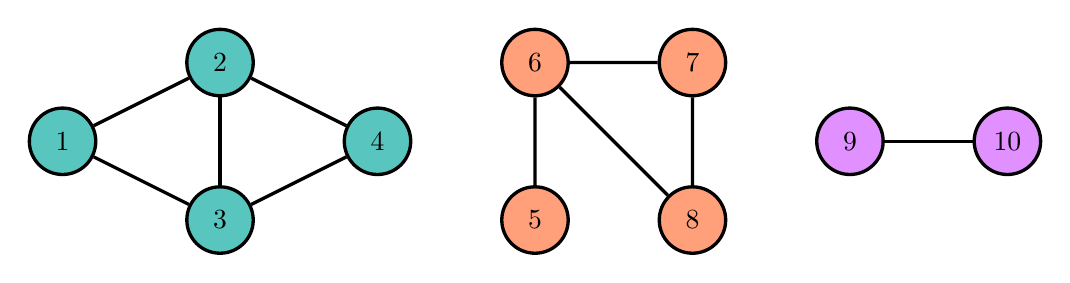
\begin{tikzpicture}[very thick,level/.style={sibling distance=70mm/#1}]
\draw (0, 0) node [vertex] (n1) {1};
\draw (2, 1) node [vertex] (n2) {2};
\draw (2, -1) node  [vertex] (n3) {3};
\draw (4, 0) node [vertex] (n4) {4};
\draw (n1) -- (n2);
\draw (n2) -- (n3);
\draw (n3) -- (n4);
\draw (n2) -- (n4);
\draw (n1) -- (n3);
\draw (6, -1) node [vertex, fill=mysalmon] (n5) {5};
\draw (6, 1) node [vertex, fill=mysalmon] (n6) {6};
\draw (8, 1) node [vertex, fill=mysalmon] (n7) {7};
\draw (8, -1) node [vertex, fill=mysalmon] (n8) {8};
\draw (n5) -- (n6) -- (n7) -- (n8) -- (n6);
\draw (10, 0) node[vertex, fill=mypurple] (n9) {9};
\draw (12, 0) node[vertex, fill=mypurple] (n10) {10};
\draw (n9) -- (n10);
\end{tikzpicture}
\end{center}

A \textit{strongly connected component} of a directed graph is a subgraph such that every vertex in the component can be reached from any other vertex in the component.

\begin{center}
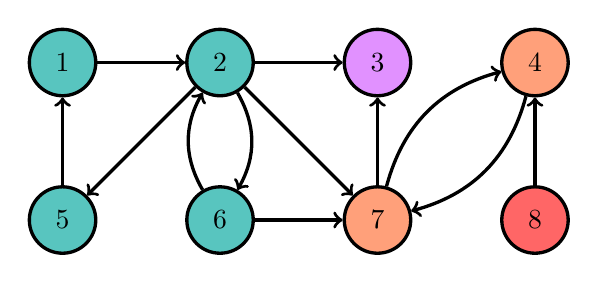
\begin{tikzpicture}[very thick,level/.style={sibling distance=70mm/#1}]
\draw (0, 0) node [vertex] (n1) {5};
\draw (2, 0) node [vertex] (n2) {6};
\draw (4, 0) node [vertex, fill=mysalmon] (n3) {7};
\draw (6, 0) node [vertex, fill=myred] (n4) {8};
\draw (0, 2) node [vertex] (m1) {1};
\draw (2, 2) node [vertex] (m2) {2};
\draw (4, 2) node [vertex, fill=mypurple] (m3) {3};
\draw (6, 2) node [vertex, fill=mysalmon] (m4) {4};
\draw[->] (m1) -- (m2);
\draw[->] (m2) -- (n1);
\draw[->] (n1) -- (m1);
\draw[->] (n2) edge [bend left] (m2);
\draw[->] (m2) edge [bend left] (n2);
\draw[->] (n2) -- (n3);
\draw[->] (m2) -- (m3);
\draw[->] (m2) -- (n3);
\draw[->] (n3) -- (m3);
\draw[->] (n3) edge [bend left] (m4);
\draw[->] (m4) edge [bend left] (n3);
\draw[->] (n4) -- (m4);
\end{tikzpicture}
\end{center}

Finding the connected components of an undirected graph is a straightforward problem, while finding the strongly connected components of a directed graph is more complicated and won't be covered in this chapter.

\subsection{Flood Fill}

Really any kind of search method solves the undirected graph connected components problem. We could use recursion with a depth-first search. To avoid using the run-time stack, we could use a queue to perform a breadth-first search. Both of these run in $O(E+V)$ time. I would recommend in general to use the BFS.

\subsection{Union-Find (Disjoint Set Union)}

The union-find data structure is another way for us to solve the connected components problem. Union-find is unique from the other search techniques in that it can process input as it is presented, edge by edge. This also means it is possible to add more edges at the end, therefore changing the graph, while still running quickly. An algorithm that works like this is an \textit{online algorithm}, while an algorithm that requires all the input data presented at the beginning is an \textit{offline algorithm}.

A natural idea for solving the connected components problem is for each vertex to maintain a pointer to another vertex it's connected to, forming a \textit{forest}, or collection of trees. To check whether two elements are in the same component, simply trace the tree up to the root by jumping up each pointer.

\begin{center}
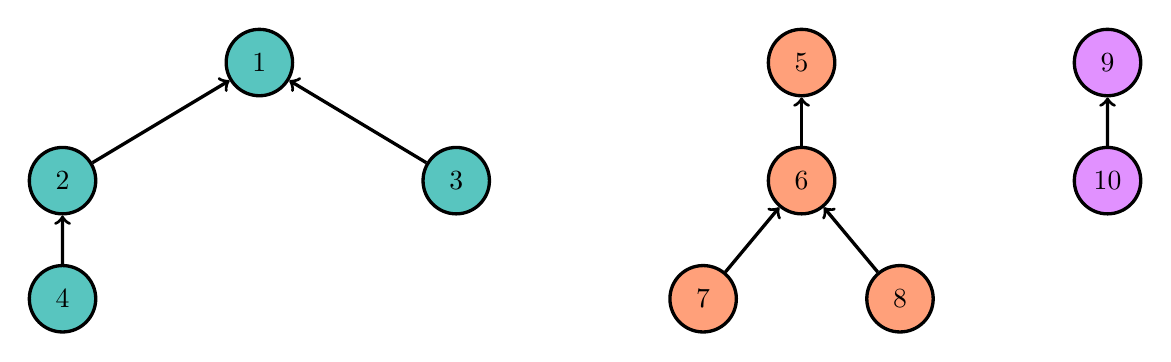
\begin{tikzpicture}[very thick,edge from parent/.style={draw,<-},level/.style={sibling distance=50mm/#1}]
\node [vertex, fill = mysalmon] (r2) {5}
  child {
      node [vertex, fill = mysalmon] {6}
      child { node [vertex, fill=mysalmon] {7} }
      child { node [vertex, fill=mysalmon] {8} }
  };

\node [vertex] [left=6cm of r2] (r1) {1}
  child {
    node [vertex] {2}
    child {
      node [vertex] {4}
    }
  }
  child {node [vertex] {3} };
  
\node [vertex, fill=mypurple] [right=3cm of r2] (r3) {9}
  child { node [vertex, fill=mypurple] {10} };
\end{tikzpicture}
\end{center}

The idea of a pointer can easily be stored within an array.

\begin{center}
{
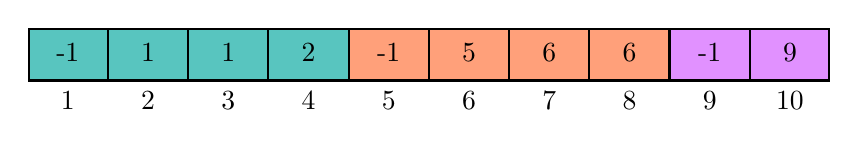
\begin{tikzpicture}[
  thick,
  myrect/.style={
    draw,
    rectangle split,
    rectangle split horizontal,
    rectangle split parts=#1,
    rectangle split part align=left,
    text width=5ex,
    text centered
    },
  mycallout/.style={
    shape=rectangle callout,
    rounded corners,
    fill=mysalmon,
    callout absolute pointer={#1},
    callout pointer width=1cm
  }  
]

\node[myrect=10, rectangle split part fill={myseagreen, myseagreen, myseagreen, myseagreen, mysalmon, mysalmon, mysalmon, mysalmon, mypurple, mypurple}]
  (array1)
  {
  					\strut -1
  \nodepart{two}	\strut 1
  \nodepart{three}	\strut 1
  \nodepart{four}	\strut 2
  \nodepart{five}	\strut -1
  \nodepart{six}	\strut 5
  \nodepart{seven}	\strut 6
  \nodepart{eight}	\strut 6
  \nodepart{nine}	\strut -1
  \nodepart{ten}	\strut 9
  };
\foreach \Valor [count=\Valori from 1] in {one ,two ,three ,four ,five ,six ,seven ,eight ,nine ,ten }
  \node[below] at (array1.\Valor south) {\Valori};

\end{tikzpicture}
}
\end{center}

We want to support two operations: $find(v)$, which returns the root of the tree containing $v$, and $union(u,v)$, which merges the components containing $u$ and $v$. This second operation is easy given the first; simply set the pointer of $find(u)$ to be $find(v)$.

$union(4, 6)$, unoptimized:

\begin{center}
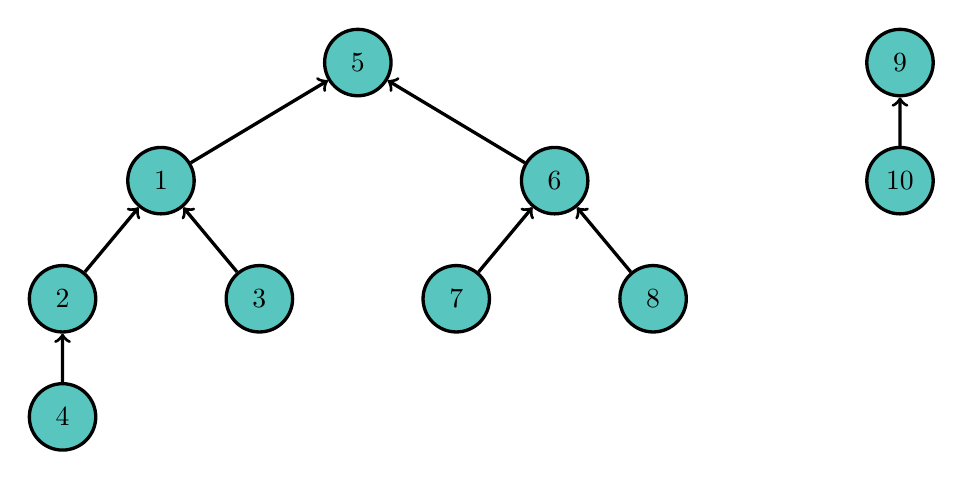
\begin{tikzpicture}[very thick,edge from parent/.style={draw,<-},level/.style={sibling distance=50mm/#1}]
\node [vertex] (r2) {5}
	child {
    node [vertex] (r1) {1}
	  child {
 	   node [vertex] {2}
  	  child {
   	   node [vertex] {4}
  	  }
	  }
 	 child {node [vertex] {3} }
  }
  child {
  node [vertex] {6}
		child { node [vertex] {7} }
   		child { node [vertex] {8} }
    };
\node [vertex] [right=6cm of r2] (r3) {9}
  child { node [vertex] {10} };
\end{tikzpicture}
\end{center}

A problem quickly arises -- the $find$ operation threatens to become linear. There are two simple things we can do to optimize this.

The first is to always add the shorter tree to the taller tree, as we want to minimize the maximum height. An easy heuristic for the height of the tree is simply the number of elements in that tree. We can keep track of the size of the tree with a second array. This heuristic is obviously not perfect, as a larger tree can be shorter than a smaller tree, but it turns out with our second optimization that this problem doesn't matter.

The second fix is to simply assign the pointer associated with $v$ to be $find(v)$ at the end of the $find$ operation. We can design $find(v)$ to recursively call $find$ on the pointer associated with $v$, so this fix sets pointers associated with nodes along the entire chain from $v$ to $find(v)$ to be $find(v)$. These two optimizations combined make the $union$ and $find$ operations $O(\alpha (V))$, where $\alpha(n)$ is the inverse Ackermann function, and for all practical values of $n$, $\alpha(n) < 5$.

$find(4)$, optimized:

\begin{center}
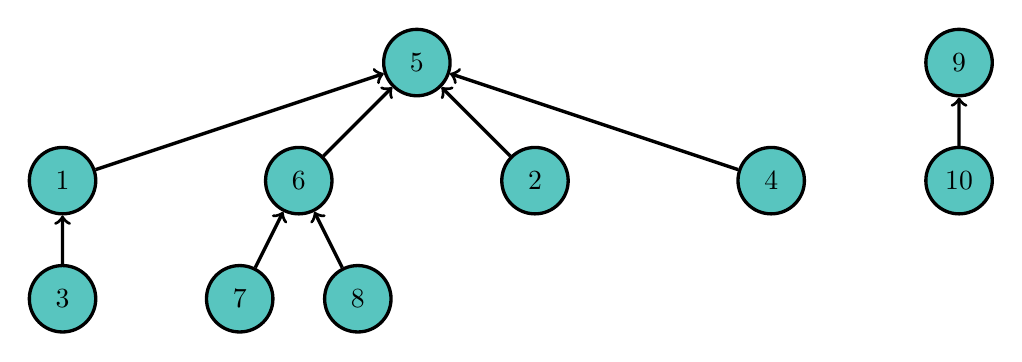
\begin{tikzpicture}[very thick,edge from parent/.style={draw,<-},level/.style={sibling distance=30mm/#1}]
\node [vertex] (r2) {5}
	child {
    node [vertex] (r1) {1}
 	 child {node [vertex] {3} }
  }
  child {
  node [vertex] {6}
		child { node [vertex] {7} }
   		child { node [vertex] {8} }
    }
  child {node[vertex] {2}}
  child {node[vertex] {4}};
\node [vertex] [right=6cm of r2] (r3) {9}
  child { node [vertex] {10} };
\end{tikzpicture}
\end{center}

\begin{algorithm}[H]
\caption{Union-Find}
%\label{}
\begin{algorithmic}
\Function{Find}{$v$}
	\If {$v$ is the root}
		\State \Return $v$
    \EndIf
    \State $parent(v) \gets \Call{Find}{parent(v)}$
    \State \Return $parent(v)$
\EndFunction
\Function{Union}{$u$, $v$}
	\State $uRoot \gets \Call{Find}{u}$
	\State $vRoot \gets \Call{Find}{v}$
    \If {$uRoot = vRoot$}
		\State \Return
	\EndIf
    \If {$size(uRoot)<size(vRoot)$}
    	\State $parent(uRoot) \gets vRoot$
        \State $size(vRoot) \gets size(uRoot) + size(vRoot)$
    \Else
    	\State $parent(vRoot) \gets uRoot$
        \State $size(uRoot) \gets size(uRoot) + size(vRoot)$
    \EndIf
\EndFunction
\end{algorithmic}
\end{algorithm}

\section{Shortest Path}

A classic. Assign nonnegative weights to each of the edges, where the weight of the edge $(u,v)$ represents the distance from $u$ to $v$. This graph can be either directed or undirected.

\subsection{Dijkstra}

Dijkstra's algorithm solves the single-source shortest path problem. From any vertex, we can compute the shortest path to each of the remaining vertices in the graph. The two formulations of Dijkstra's algorithm run in $O(V^2)$ or $O(E\log{V})$ time, whichever one suits us better. Note that it is possible to do better than $O(E\log{V})$ using a Fibonacci heap. The former works nicely on dense graphs, as $E \approx V^2$, while the latter works better on sparse graphs, as $E \approx V$.

For every vertex $v$ in the graph, we keep track of the shortest known distance $dist(v)$ from the source to $v$, a boolean $visited(v)$ to keep track of which nodes we ``visited,'' and a pointer to the previous node in the shortest known path $prev(v)$ so that we can trace the shortest path once the algorithm finishes.

Dijkstra iteratively ``visits'' the next nearest vertex, updating the distances to that vertex's neighbors if necessary. Therefore, at any step, we have the first however-many nearest vertices to the source, which we call ``visited'' and for which the shortest path is known. We also have the shortest path to all the remaining vertices that stays within the ``visited'' vertices besides for the very last edge, if such a path exists. We claim that the known distance to the closest vertex that has not yet been visited is the shortest distance. We can then ``visit'' that vertex. It shouldn't be hard to prove that this algorithm indeed calculates the shortest path.

The $O(V^2)$ implementation immediately follows.

\begin{algorithm}[H]
\caption{Dijkstra}
\begin{algorithmic}
\ForAll{vertices $v$}
	\State $dist(v) \gets \infty$
	\State $visited(v) \gets 0$
    \State $prev(v) \gets -1$
\EndFor
\State $dist(src) \gets 0$
\While{$\exists v$ s.t. $visited(v)=0$}
	\State $v \equiv v$ s.t. $visited(v)=0$ with min $dist(v)$
    \State $visited(v) \gets 1$
	\ForAll{neighbors $u$ of $v$}
    	\If{$visited(u) = 0$}
    		\State $alt \gets dist(v) + weight(v, u)$
			\If{$alt < dist(u)$}
				\State $dist(u) \gets alt$
   	        	\State $prev(u) \gets v$
			\EndIf
        \EndIf
    \EndFor
\EndWhile
\end{algorithmic}
\end{algorithm}

\begin{center}
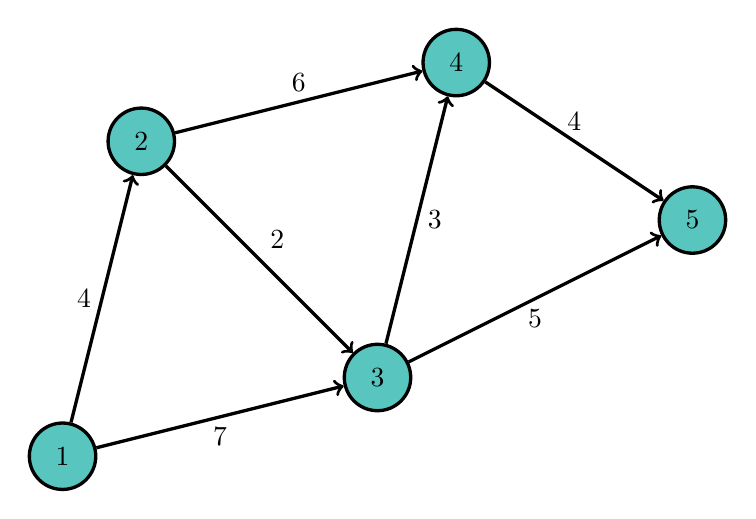
\begin{tikzpicture}[very thick,edge from parent/.style={draw,<-},level/.style={sibling distance=30mm/#1}]
\draw (0, 0) node [vertex] (v1) {1};
\draw (1, 4) node [vertex] (v2) {2};
\draw (4, 1) node [vertex] (v3) {3};
\draw (5, 5) node [vertex] (v4) {4};
\draw (8, 3) node [vertex] (v5) {5};
\draw[->] (v1) -- (v2) node[midway, left] {4};
\draw[->] (v2) -- (v3) node[midway, above right] {2};
\draw[->] (v1) -- (v3) node[midway, below] {7};
\draw[->] (v2) -- (v4) node[midway, above] {6};
\draw[->] (v3) -- (v4) node[midway, right] {3};
\draw[->] (v3) -- (v5) node[midway, below] {5};
\draw[->] (v4) -- (v5) node[midway, above] {4};
\end{tikzpicture}
\end{center}

Let's run Dijkstra's algorithm on the above graph with vertex 1 as the source. We first set all the distances besides the source to be $\infty$.

\begin{center}
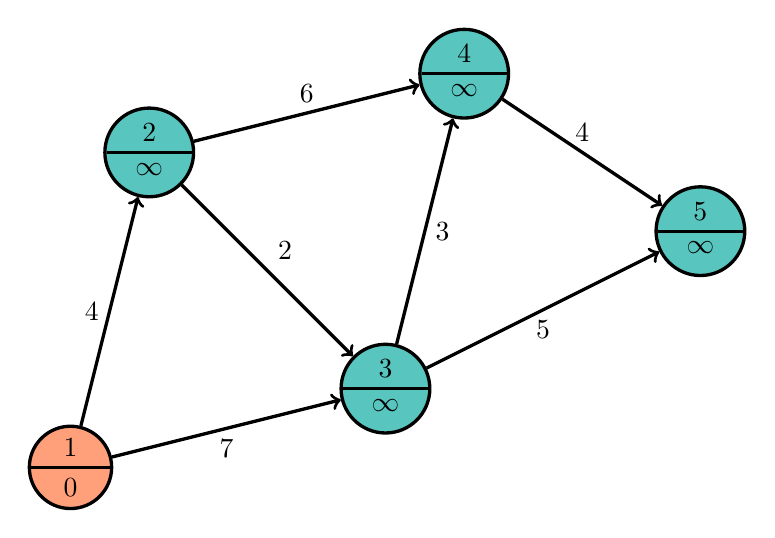
\begin{tikzpicture}[very thick,edge from parent/.style={draw,<-},level/.style={sibling distance=30mm/#1}]
\draw (0, 0) node [splitvertex, fill=mysalmon] (v1) {1\nodepart{lower}0};
\draw (1, 4) node [splitvertex] (v2) {2\nodepart{lower}$\infty$};
\draw (4, 1) node [splitvertex] (v3) {3\nodepart{lower}$\infty$};
\draw (5, 5) node [splitvertex] (v4) {4\nodepart{lower}$\infty$};
\draw (8, 3) node [splitvertex] (v5) {5\nodepart{lower}$\infty$};
\draw[->] (v1) -- (v2) node[midway, left] {4};
\draw[->] (v2) -- (v3) node[midway, above right] {2};
\draw[->] (v1) -- (v3) node[midway, below] {7};
\draw[->] (v2) -- (v4) node[midway, above] {6};
\draw[->] (v3) -- (v4) node[midway, right] {3};
\draw[->] (v3) -- (v5) node[midway, below] {5};
\draw[->] (v4) -- (v5) node[midway, above] {4};
\end{tikzpicture}
\end{center}

Now, we continue choosing the closest unvisited node, mark it as visited, and and update its neighbors.

\begin{center}
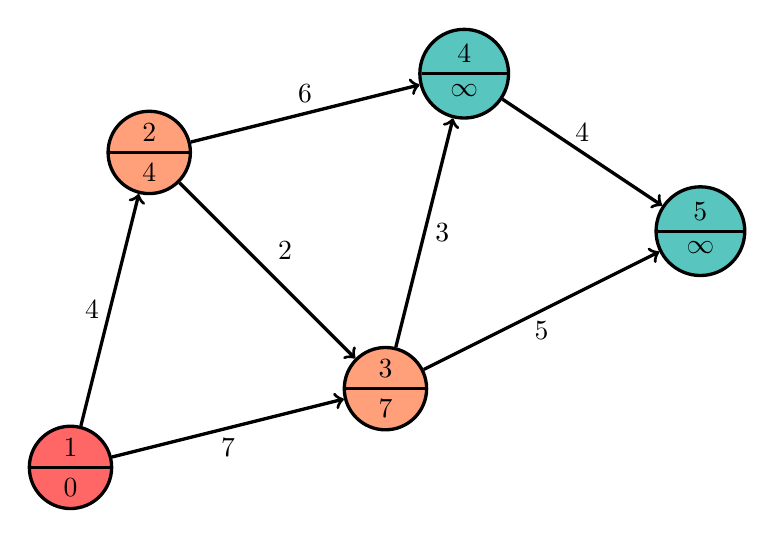
\begin{tikzpicture}[very thick,edge from parent/.style={draw,<-},level/.style={sibling distance=30mm/#1}]
\draw (0, 0) node [splitvertex, fill=myred] (v1) {1\nodepart{lower}0};
\draw (1, 4) node [splitvertex, fill=mysalmon] (v2) {2\nodepart{lower}4};
\draw (4, 1) node [splitvertex, fill=mysalmon] (v3) {3\nodepart{lower}7};
\draw (5, 5) node [splitvertex] (v4) {4\nodepart{lower}$\infty$};
\draw (8, 3) node [splitvertex] (v5) {5\nodepart{lower}$\infty$};
\draw[->] (v1) -- (v2) node[midway, left] {4};
\draw[->] (v2) -- (v3) node[midway, above right] {2};
\draw[->] (v1) -- (v3) node[midway, below] {7};
\draw[->] (v2) -- (v4) node[midway, above] {6};
\draw[->] (v3) -- (v4) node[midway, right] {3};
\draw[->] (v3) -- (v5) node[midway, below] {5};
\draw[->] (v4) -- (v5) node[midway, above] {4};
\end{tikzpicture}
\end{center}

\begin{center}
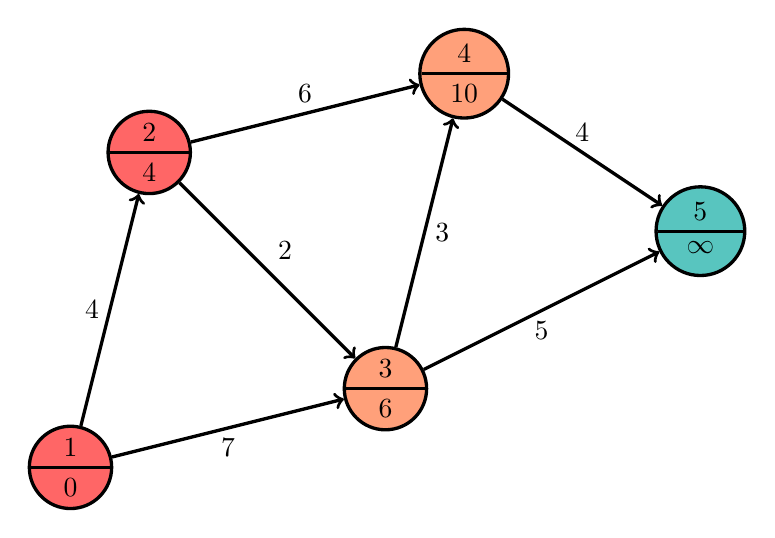
\begin{tikzpicture}[very thick,edge from parent/.style={draw,<-},level/.style={sibling distance=30mm/#1}]
\draw (0, 0) node [splitvertex, fill=myred] (v1) {1\nodepart{lower}0};
\draw (1, 4) node [splitvertex, fill=myred] (v2) {2\nodepart{lower}4};
\draw (4, 1) node [splitvertex, fill=mysalmon] (v3) {3\nodepart{lower}6};
\draw (5, 5) node [splitvertex, fill=mysalmon] (v4) {4\nodepart{lower}10};
\draw (8, 3) node [splitvertex] (v5) {5\nodepart{lower}$\infty$};
\draw[->] (v1) -- (v2) node[midway, left] {4};
\draw[->] (v2) -- (v3) node[midway, above right] {2};
\draw[->] (v1) -- (v3) node[midway, below] {7};
\draw[->] (v2) -- (v4) node[midway, above] {6};
\draw[->] (v3) -- (v4) node[midway, right] {3};
\draw[->] (v3) -- (v5) node[midway, below] {5};
\draw[->] (v4) -- (v5) node[midway, above] {4};
\end{tikzpicture}
\end{center}

\begin{center}
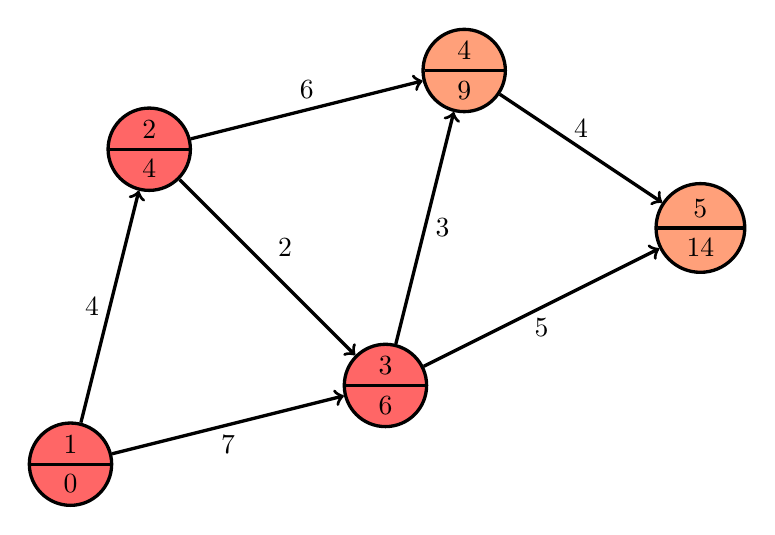
\begin{tikzpicture}[very thick,edge from parent/.style={draw,<-},level/.style={sibling distance=30mm/#1}]
\draw (0, 0) node [splitvertex, fill=myred] (v1) {1\nodepart{lower}0};
\draw (1, 4) node [splitvertex, fill=myred] (v2) {2\nodepart{lower}4};
\draw (4, 1) node [splitvertex, fill=myred] (v3) {3\nodepart{lower}6};
\draw (5, 5) node [splitvertex, fill=mysalmon] (v4) {4\nodepart{lower}9};
\draw (8, 3) node [splitvertex, fill=mysalmon] (v5) {5\nodepart{lower}14};
\draw[->] (v1) -- (v2) node[midway, left] {4};
\draw[->] (v2) -- (v3) node[midway, above right] {2};
\draw[->] (v1) -- (v3) node[midway, below] {7};
\draw[->] (v2) -- (v4) node[midway, above] {6};
\draw[->] (v3) -- (v4) node[midway, right] {3};
\draw[->] (v3) -- (v5) node[midway, below] {5};
\draw[->] (v4) -- (v5) node[midway, above] {4};
\end{tikzpicture}
\end{center}

\begin{center}
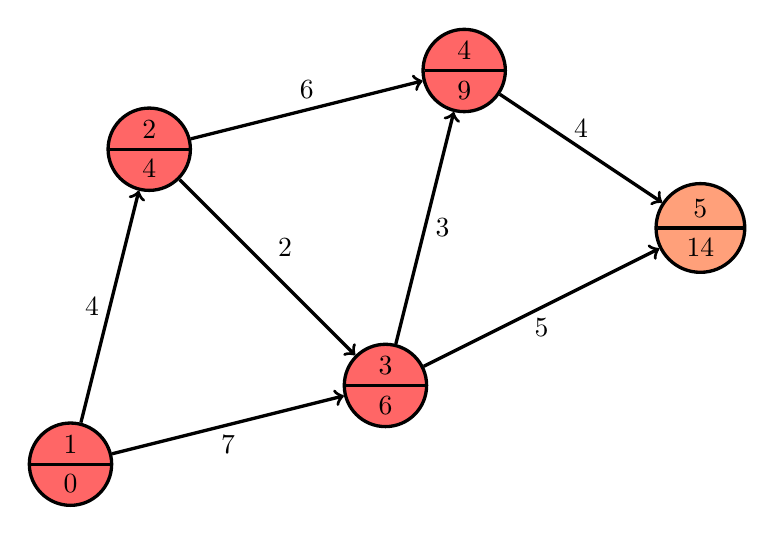
\begin{tikzpicture}[very thick,edge from parent/.style={draw,<-},level/.style={sibling distance=30mm/#1}]
\draw (0, 0) node [splitvertex, fill=myred] (v1) {1\nodepart{lower}0};
\draw (1, 4) node [splitvertex, fill=myred] (v2) {2\nodepart{lower}4};
\draw (4, 1) node [splitvertex, fill=myred] (v3) {3\nodepart{lower}6};
\draw (5, 5) node [splitvertex, fill=myred] (v4) {4\nodepart{lower}9};
\draw (8, 3) node [splitvertex, fill=mysalmon] (v5) {5\nodepart{lower}14};
\draw[->] (v1) -- (v2) node[midway, left] {4};
\draw[->] (v2) -- (v3) node[midway, above right] {2};
\draw[->] (v1) -- (v3) node[midway, below] {7};
\draw[->] (v2) -- (v4) node[midway, above] {6};
\draw[->] (v3) -- (v4) node[midway, right] {3};
\draw[->] (v3) -- (v5) node[midway, below] {5};
\draw[->] (v4) -- (v5) node[midway, above] {4};
\end{tikzpicture}
\end{center}

\begin{center}
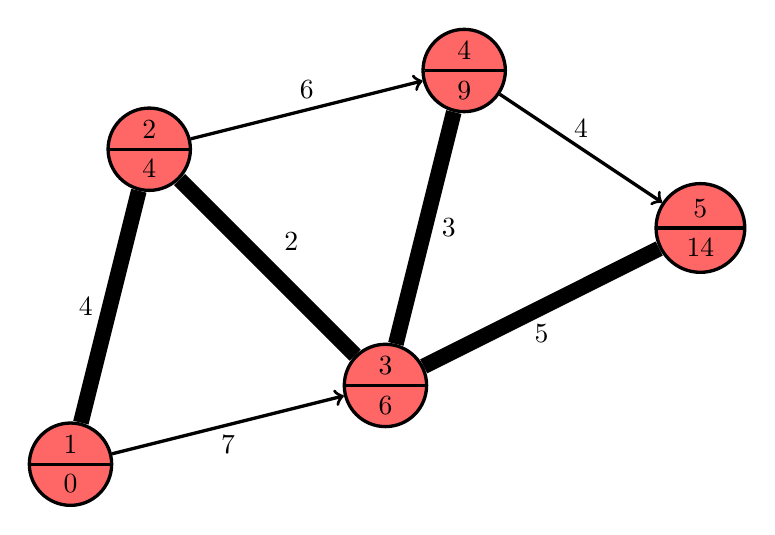
\begin{tikzpicture}[very thick,edge from parent/.style={draw,<-},level/.style={sibling distance=30mm/#1}]
\draw (0, 0) node [splitvertex, fill=myred] (v1) {1\nodepart{lower}0};
\draw (1, 4) node [splitvertex, fill=myred] (v2) {2\nodepart{lower}4};
\draw (4, 1) node [splitvertex, fill=myred] (v3) {3\nodepart{lower}6};
\draw (5, 5) node [splitvertex, fill=myred] (v4) {4\nodepart{lower}9};
\draw (8, 3) node [splitvertex, fill=myred] (v5) {5\nodepart{lower}14};
\draw[line width=2mm] (v1) -- (v2) node[midway, left] {4};
\draw[line width=2mm] (v2) -- (v3) node[midway, above right] {2};
\draw[->] (v1) -- (v3) node[midway, below] {7};
\draw[->] (v2) -- (v4) node[midway, above] {6};
\draw[line width=2mm] (v3) -- (v4) node[midway, right] {3};
\draw[line width=2mm] (v3) -- (v5) node[midway, below] {5};
\draw[->] (v4) -- (v5) node[midway, above] {4};
\end{tikzpicture}
\end{center}

The slow part of the $O(V^2)$ formulation is the linear search for the vertex $v$ with the minimum $dist(v)$. We happen to have a data structure that resolves this problem -- a binary heap. The main problem with using the standard library heap is having repeated vertices in the heap. We could just ignore this problem and discard visited vertices as they come out of the heap. Alternatively, we could choose never to have repeated vertices in the heap. To do this, we need to be able to change the value of the distances once they are already in the heap, or \textit{decrease-key}. This is a pretty simple function to add, however, if you have a heap already coded. Either way, we achieve $O(E \log{V})$, as we do $E+V$ updates to our heap, each costing $O(V)$.

\subsection{Floyd-Warshall}

Dijkstra is nice when we are dealing with edges with nonnegative weights and are looking for the distances from one vertex to all the others. Floyd-Warshall solves the shortest path problem for all pairs of vertices in $O(V^3)$ time, which is faster than $V$ single-source Dijkstra runs on a dense graph. Floyd-Warshall works even if some edge weights are negative but not if the graph has a negative cycle.

\begin{algorithm}[H]
\caption{Floyd-Warshall}
\begin{algorithmic}
\ForAll{vertices $v$}
	\State $dist(v,v)=0$
\EndFor
\ForAll{edges $(u,v)$}
	\State $dist(u,v)=weight(u,v)$
\EndFor
\ForAll{vertices $k$}
	\ForAll{vertices $i$}
    	\ForAll{vertices $j$}
        	\If{$dist(i,j) > dist(i,k)+dist(k,j)$}
            	\State $dist(i,j) \gets dist(i,k)+dist(k,j)$
            \EndIf
        \EndFor
    \EndFor
\EndFor
\end{algorithmic}
\end{algorithm}

\subsection{Bellman-Ford}

Bellman-Ford is a single-source $O(VE)$ shortest path algorithm that works when edge weights can be negative. It is preferable to Floyd-Warshall when the graph is sparse and we only need the answer for one source. Like Floyd-Warshall, the algorithm fails if the graph contains a negative cycle, but the algorithm is still useful for detecting negative cycles.

The idea here is the shortest path, assuming no negative cycles, has length at most $V-1$.

\begin{algorithm}[H]
\caption{Bellman-Ford}
\begin{algorithmic}
\ForAll{vertices $v$}
	\State $dist(v)\gets\infty$
    \State $prev(v)=\gets -1$
\EndFor
\State $dist(src) \gets 0$
\For{$i\equiv 1,V-1$}
	\ForAll{edges $(u,v)$}
		\If{$dist(u)+weight(u,v) < dist(v)$}
    	    \State $dist(v) \gets dist(u)+weight(u,v)$
	        \State $prev(v) \gets u$
        \EndIf
	\EndFor
\EndFor
\ForAll{edges $(u,v)$}
	\Comment{check for negative cycles}
	\If{$dist(u)+weight(u,v) < dist(v)$}
   	    \State{negative cycle detected}
	\EndIf
\EndFor
\end{algorithmic}
\end{algorithm}

\section{Minimum Spanning Tree}

Consider a connected, undirected graph. A \textit{spanning tree} is a subgraph that is a tree and contains every vertex in the original graph. A \textit{minimum spanning tree} is a spanning tree such that the sum of the edge weights of the tree is minimized. Finding the minimum spanning tree uses many of the same ideas discussed earlier.

\begin{center}
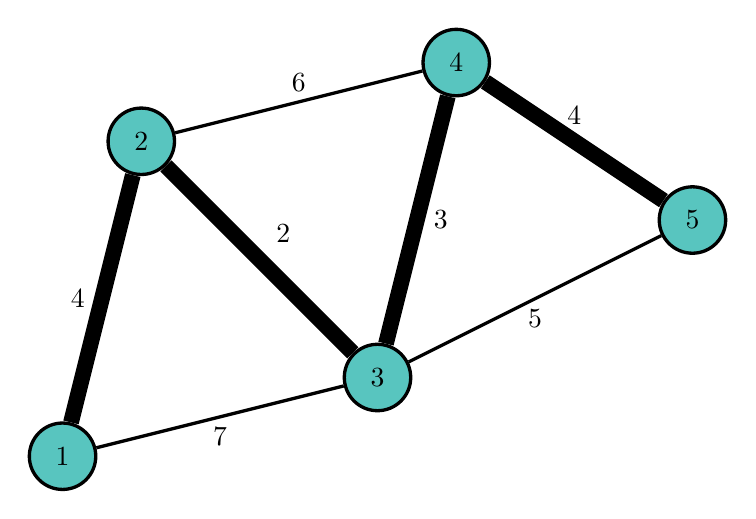
\begin{tikzpicture}[very thick,edge from parent/.style={draw,<-},level/.style={sibling distance=30mm/#1}]
\draw (0, 0) node [vertex] (v1) {1};
\draw (1, 4) node [vertex] (v2) {2};
\draw (4, 1) node [vertex] (v3) {3};
\draw (5, 5) node [vertex] (v4) {4};
\draw (8, 3) node [vertex] (v5) {5};
\draw[line width=2mm] (v1) -- (v2) node[midway, left] {4};
\draw[line width=2mm] (v2) -- (v3) node[midway, above right] {2};
\draw (v1) -- (v3) node[midway, below] {7};
\draw (v2) -- (v4) node[midway, above] {6};
\draw[line width=2mm] (v3) -- (v4) node[midway, right] {3};
\draw (v3) -- (v5) node[midway, below] {5};
\draw[line width=2mm] (v4) -- (v5) node[midway, above] {4};
\end{tikzpicture}
\end{center}

\subsection{Prim}

Prim's algorithm for finding the minimum spanning tree is very similar to Dijkstra's algorithm for finding the shortest path. Like Dijkstra, it iteratively adds a new vertex at a time to build a tree. The only difference is $dist(v)$ stores the shortest distance from \textit{any} visited node instead of the source.

\begin{algorithm}[H]
\caption{Prim}
\begin{algorithmic}
\ForAll{vertices $v$}
	\State $dist(v) \gets \infty$
	\State $visited(v) \gets 0$
    \State $prev(v) \gets -1$
\EndFor
\State $dist(src) \gets 0$
\While{$\exists v$ s.t. $visited(v)=0$}
	\State $v \equiv v$ s.t. $visited(v)=0$ with min $dist(v)$
    \State $visited(v) \gets 1$
	\ForAll{neighbors $u$ of $v$}
    	\If{$visited(u) = 0$}
			\If{$weight(v, u) < dist(u)$}
				\State $dist(u) \gets weight(v, u)$
   	        	\State $prev(u) \gets v$
			\EndIf
        \EndIf
    \EndFor
\EndWhile
\end{algorithmic}
\end{algorithm}

The proof of correctness is left as an exercise. The complexity of this algorithm depends on how the minimum unvisited vertex is calculated. Using the same approaches as Dijkstra, we can achieve $O(V^2)$ or $O(E \log{V})$.

\subsection{Kruskal}

While Prim greedily adds vertices to the tree, Kruskal's algorithm greedily adds edges. It iterates over all the edges, sorted by weight. We need to watch out for adding a cycle, breaking the tree structure, which means we need to keep track of each vertex's connected component. If an edge connects two vertices from the same connected component, we don't want to add it to our tree. However, we have a union-find algorithm that works perfectly for this.

\begin{algorithm}[H]
\caption{Kruskal}
\begin{algorithmic}
\ForAll{edges $(u,v)$ in sorted order}
	\If{$\Call{Find}{u} \not= \Call{Find}{v}$}
		\State add $(u,v)$ to spanning tree
		\State $\Call{Union}{u,v}$
	\EndIf
\EndFor
\end{algorithmic}
\end{algorithm}

This algorithm requires a sort of the edges and thus has complexity $O(E \log{E}) = O(E \log{V})$.

\section{Eulerian Tour}

An \textit{Eulerian tour} of a graph is a path that traverses every edge exactly once. If the tour ends exactly where it started, it is called an \textit{Eulerian circuit}. A graph has an Eulerian circuit if it is connected and every vertex has even degree. A graph has an Eulerian path if it is connected and all vertices but exactly two have even degrees. The mathematical proofs for these graph properties hinge on the idea that removing a cycle from the graph maintains the Eulerian property. We construct an Eulerian tour by appealing to this idea.

\begin{algorithm}[H]
\caption{Eulerian Tour}
\begin{algorithmic}
\Function{FindTour}{$v$}
\While{$v$ has a neighbor $u$}
	\State delete edge $(v,u)$
	\State \Call{FindTour}{$u$}
	\Comment{\Call{FindTour}{$u$} must trace a circuit back to $v$}
\EndWhile
\State add $v$ to tour
\EndFunction
\end{algorithmic}
\end{algorithm}

It is not preferable to use the run-time stack; we can use our own stack if necessary.

If the graph contains an Eulerian circuit, we call this function on any vertex we like. If it contains an Eulerian path, we call this function on one of the vertices with odd degree.


\chapter{Complex Ideas and Data Structures}

Here we build on previous material to introduce more complex ideas that are useful for solving USACO Gold problems and beyond.

\section{Dynamic Programming over Subsets ($n2^n$ DP)}

We've already covered how dynamic programming can turn exponential solutions into polynomial solutions, but it can also help turn factorial solutions into exponential. Problems where the bound on $n$ is 20, for example, signal that an exponential solution is the one required. Consider the following problem:

(USACO December 2014, guard)
Farmer John and his herd are playing frisbee.  Bessie throws the
frisbee down the field, but it's going straight to Mark the field hand
on the other team!  Mark has height $H$ ($1 \le H \le 1,000,000,000$), but
there are $N$ cows on Bessie's team gathered around Mark ($2 \le N \le 20$).
They can only catch the frisbee if they can stack up to be at least as
high as Mark.  Each of the $N$ cows has a height, weight, and strength.
A cow's strength indicates the maximum amount of total weight of the
cows that can be stacked above her.  

Given these constraints, Bessie wants to know if it is possible for
her team to build a tall enough stack to catch the frisbee, and if so,
what is the maximum safety factor of such a stack.  The safety factor
of a stack is the amount of weight that can be added to the top of the
stack without exceeding any cow's strength.

We can try the $O(N!)$ brute force, trying every permutation of cows possible. However, this is far too slow. $N \le 20$ hints at an exponential solution, so we think of trying every possible subset of the cows. Given a subset $S$ of cows, the height reached is the same, so perhaps we sort the subset by strength, and put the strongest cow on the bottom. We see that this greedy approach fails: suppose that the first cow has weight 1 and strength 3 and the second cow has weight 4 and strength 2. Greedy would tell us to put the first cow on the bottom, but this fails, while putting the second cow on the bottom succeeds.

When greedy fails, the next strategy we look at is dynamic programming. To decide whether $S$ is stable, we have to find whether there exists a cow $j$ in $S$ that can support the weight of all the other cows in $S$. But how do we know whether the set $S \setminus \{j\}$ is stable? This is where dynamic programming comes in.

This leads to a $O(N 2^N)$ solution. This seems like a pain to code iteratively, but there is a nice fact about subsets: there is a cute bijection from the subsets of $\{0,1,2, \ldots, N-1\}$ to the integers from 0 to $2^N - 1$. That is, the subset $\{0,2,5,7\}$ maps to $2^0 + 2^2 + 2^5 + 2^7 = 165$ in the bijection. We call this technique \textit{masking}. We require all the subsets of $S$ to be processed before $S$ is processed, but that property is also handled by our bijection, since subtracting a power of 2 from a number decreases it. With a little knowledge of bit operators, this can be handled easily.

\noindent \begin{minipage}{\textwidth}
\begin{algorithmic}
\For{$i\gets 0, 2^N-1$}
	\Comment $i$ represents the subset $S$
	\State $dp(i) \gets -1$
	\ForAll{$j \in S$}
		\Comment $j \in S$ satisfy \texttt{i \& (1 << j) != 0}
		\State $alt \gets \min(dp(i-2^j), strength(j) - \sum_{k \in S \setminus \{j\}} weight(k))$
		\If{$dp(i) < alt$}
			\State $dp(i) \gets alt$
		\EndIf
	\EndFor
\EndFor
\end{algorithmic}
\end{minipage}

\texttt{\&} is the bitwise and function, while \texttt{<<} is the left shift operator.

\section{$\sqrt{n}$ Bucketing}

$\sqrt{n}$ bucketing is a relatively straightforward idea -- given $n$ elements $\{a_i\}_{i=1}^n$ in a sequence, we group them into $\sqrt{n}$ equal-sized buckets. The motivation for arranging elements like this is to support an operation called a \textit{range query}.

Let's take a concrete example. Suppose we want to support two operations:

\begin{itemize}
\item
$update(i, x)$ -- increment the value of $a_i$ by $x$

\item
$query(i, j)$ -- return $\sum_{k=i}^j a_k$.
\end{itemize}

Suppose we simply stored the sequence in an array. $update$ then becomes an $O(1)$ operation, but $query$ is $O(n)$.

\begin{center}
{
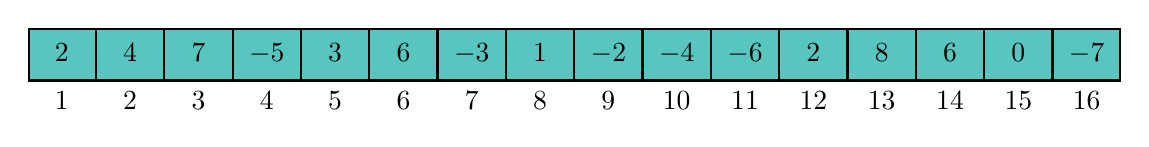
\begin{tikzpicture}[
  thick,
  myrect/.style={
    draw,
    fill=myseagreen,
    rectangle split,
    rectangle split horizontal,
    rectangle split parts=#1,
    rectangle split part align=left,
    text width=4ex,
    text centered
    }
]

\node[myrect=16]
  (array)
  {
  					\strut 2
  \nodepart{two}	\strut 4
  \nodepart{three}	\strut 7
  \nodepart{four}	\strut $-5$
  \nodepart{five}	\strut 3
  \nodepart{six}	\strut 6
  \nodepart{seven}	\strut $-3$
  \nodepart{eight}	\strut 1
  \nodepart{nine}	\strut $-2$
  \nodepart{ten}	\strut $-4$
  \nodepart{eleven}	\strut $-6$
  \nodepart{twelve}	\strut 2
  \nodepart{thirteen}	\strut 8
  \nodepart{fourteen}	\strut 6
  \nodepart{fifteen}	\strut 0
  \nodepart{sixteen}	\strut $-7$
  };
\foreach \Valor [count=\Valori from 1] in {one ,two ,three , four , five , six , seven , eight , nine , ten , eleven , twelve , thirteen , fourteen , fifteen , sixteen }
  \node[below] at (array.\Valor south) {\Valori};

\end{tikzpicture}
}
\end{center}

Another natural approach would be to store in a separate array the sum of the first $i$ terms in the sequence for every index $i$, or store the \textit{prefix sums}.

\begin{center}
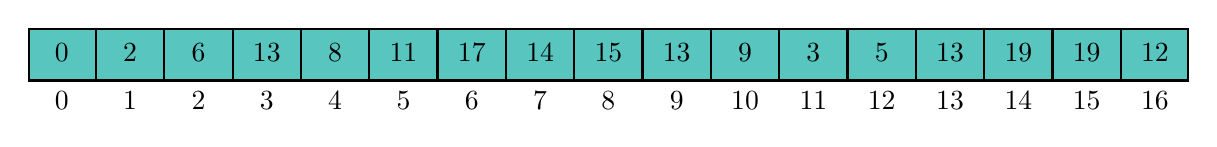
\begin{tikzpicture}[
  thick,
  myrect/.style={
    draw,
    fill=myseagreen,
    rectangle split,
    rectangle split horizontal,
    rectangle split parts=#1,
    rectangle split part align=left,
    text width=4ex,
    text centered
    }
]

\node[myrect=17]
  (array)
  {
  					\strut 0
  \nodepart{two}	\strut 2
  \nodepart{three}	\strut 6
  \nodepart{four}	\strut 13
  \nodepart{five}	\strut 8
  \nodepart{six}	\strut 11
  \nodepart{seven}	\strut 17
  \nodepart{eight}	\strut 14
  \nodepart{nine}	\strut 15
  \nodepart{ten}	\strut 13
  \nodepart{eleven}	\strut 9
  \nodepart{twelve}	\strut 3
  \nodepart{thirteen}	\strut 5
  \nodepart{fourteen}	\strut 13
  \nodepart{fifteen}	\strut 19
  \nodepart{sixteen}	\strut 19
  \nodepart{seventeen}	\strut 12
  };
\foreach \Valor [count=\Valori from 0] in {one ,two ,three , four , five , six , seven , eight , nine , ten , eleven , twelve , thirteen , fourteen , fifteen , sixteen , seventeen }
  \node[below] at (array.\Valor south) {\Valori};

\end{tikzpicture}

\end{center}

Now $query$ becomes an $O(1)$ operation, as we can simply subtract two elements in the array to answer a query. Unfortunately, $update$ becomes $O(n)$, as changing the value of an element in the beginning of the sequence forces us to change almost all the values in the prefix sum array.

We can still use this idea, though... what we are looking for is some way to group values into sums such that we only need to change a small number of the sums to $update$ and only require a small number of them to $query$.

This leads us directly to a $\sqrt{n}$ bucketing solution. Let's group the 16 elements into 4 groups.

\begin{center}
{
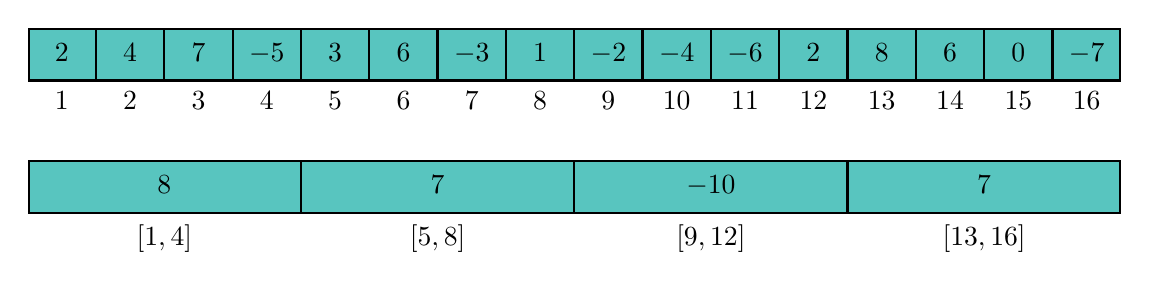
\begin{tikzpicture}[
  thick,
  myrect/.style={
    draw,
    fill=myseagreen,
    rectangle split,
    rectangle split horizontal,
    rectangle split parts=#1,
    rectangle split part align=left,
    text width=4ex,
    text centered
    }
]

\node[myrect=16]
  (array2)
  {
  					\strut 2
  \nodepart{two}	\strut 4
  \nodepart{three}	\strut 7
  \nodepart{four}	\strut $-5$
  \nodepart{five}	\strut 3
  \nodepart{six}	\strut 6
  \nodepart{seven}	\strut $-3$
  \nodepart{eight}	\strut 1
  \nodepart{nine}	\strut $-2$
  \nodepart{ten}	\strut $-4$
  \nodepart{eleven}	\strut $-6$
  \nodepart{twelve}	\strut 2
  \nodepart{thirteen}	\strut 8
  \nodepart{fourteen}	\strut 6
  \nodepart{fifteen}	\strut 0
  \nodepart{sixteen}	\strut $-7$
  };
\foreach \Valor [count=\Valori from 1] in {one ,two ,three , four , five , six , seven , eight , nine , ten , eleven , twelve , thirteen , fourteen , fifteen , sixteen }
  \node[below] at (array2.\Valor south) {\Valori};

\node[myrect=4, text width=21.2ex] [below=of array2]
  (array)
  {
  					\strut 8
  \nodepart{two}	\strut 7
  \nodepart{three}	\strut $-10$
  \nodepart{four}	\strut 7
  };

\node[below] at (array.one south) {$[1,4]$};
\node[below] at (array.two south) {$[5,8]$};
\node[below] at (array.three south) {$[9,12]$};
\node[below] at (array.four south) {$[13,16]$};
\end{tikzpicture}
}
\end{center}

We'll keep track of the total sum of each group. Now, if we want to update a value, we need to change only two values -- the value of that element in the original array and the total sum of the bucket it is in. When we query a range, we'll take advantage of the sum of the bucket when we can. Highlighted are the numbers we'll need for $query(7,15)$.

\begin{center}
{
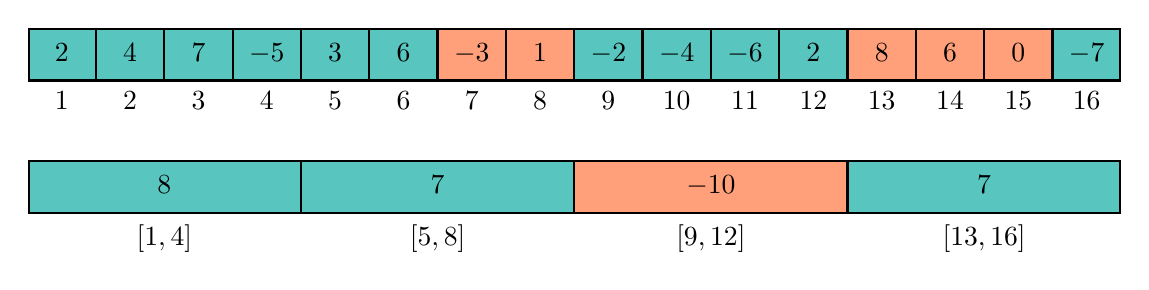
\begin{tikzpicture}[
  thick,
  myrect/.style={
    draw,
    rectangle split,
    rectangle split horizontal,
    rectangle split parts=#1,
    rectangle split part align=left,
    text width=4ex,
    text centered
    }
]

\node[myrect=16, rectangle split part fill={myseagreen, myseagreen, myseagreen, myseagreen, myseagreen, myseagreen, mysalmon, mysalmon, myseagreen, myseagreen, myseagreen, myseagreen, mysalmon, mysalmon, mysalmon, myseagreen}]
  (array2)
  {
  					\strut 2
  \nodepart{two}	\strut 4
  \nodepart{three}	\strut 7
  \nodepart{four}	\strut $-5$
  \nodepart{five}	\strut 3
  \nodepart{six}	\strut 6
  \nodepart{seven}	\strut $-3$
  \nodepart{eight}	\strut 1
  \nodepart{nine}	\strut $-2$
  \nodepart{ten}	\strut $-4$
  \nodepart{eleven}	\strut $-6$
  \nodepart{twelve}	\strut 2
  \nodepart{thirteen}	\strut 8
  \nodepart{fourteen}	\strut 6
  \nodepart{fifteen}	\strut 0
  \nodepart{sixteen}	\strut $-7$
  };
\foreach \Valor [count=\Valori from 1] in {one ,two ,three , four , five , six , seven , eight , nine , ten , eleven , twelve , thirteen , fourteen , fifteen , sixteen }
  \node[below] at (array2.\Valor south) {\Valori};

\node[myrect=4, text width=21.2ex, rectangle split part fill={myseagreen, myseagreen, mysalmon, myseagreen}] [below=of array2]
  (array)
  {
  					\strut 8
  \nodepart{two}	\strut 7
  \nodepart{three}	\strut $-10$
  \nodepart{four}	\strut 7
  };

\node[below] at (array.one south) {$[1,4]$};
\node[below] at (array.two south) {$[5,8]$};
\node[below] at (array.three south) {$[9,12]$};
\node[below] at (array.four south) {$[13,16]$};

\end{tikzpicture}
}
\end{center}

Querying requires access to at most $\sqrt{n}$ bucket sums and $2(\sqrt{n}-1)$ individual values. Therefore we have $O(\sqrt{n})$ query and $O(1)$ update. We are able to improve $O(\sqrt{n})$ update to $O(1)$ because of nice properties of the $+$ operator. This is not always the case for range queries: suppose, for instance, we needed to find the minimum element on a range.

It is often the case that $O(\sqrt{n})$ bounds can be improved to $O(\log{n})$ using more complex data structures like segment trees and more complex ideas like $2^n$ jump pointers, both of which are covered in this chapter. These are, however, more complicated to implement and as such are often comparable in runtime in the contest environment. Steven Hao is notorious for using crude $\sqrt{n}$ bucketing algorithms to solve problems that should have required tighter algorithm complexities. $\sqrt{n}$ bucketing is a crude yet powerful idea; always keep it in the back of your mind.

\section{Segment Tree}

It turns out for our specific sum problem that we can do as good as $O(\log{n})$ with a \textit{segment tree}, or \textit{range tree}, or \textit{augmented static BBST}. The essential idea is still the same -- we want to group elements in some way that allows us to update and query efficiently.

As the name ``tree'' suggests, we draw inspiration from a binary structure. Let's build a tree on top of the array, where each node keeps track of the sum of the numbers associated with its children.

\begin{center}
{
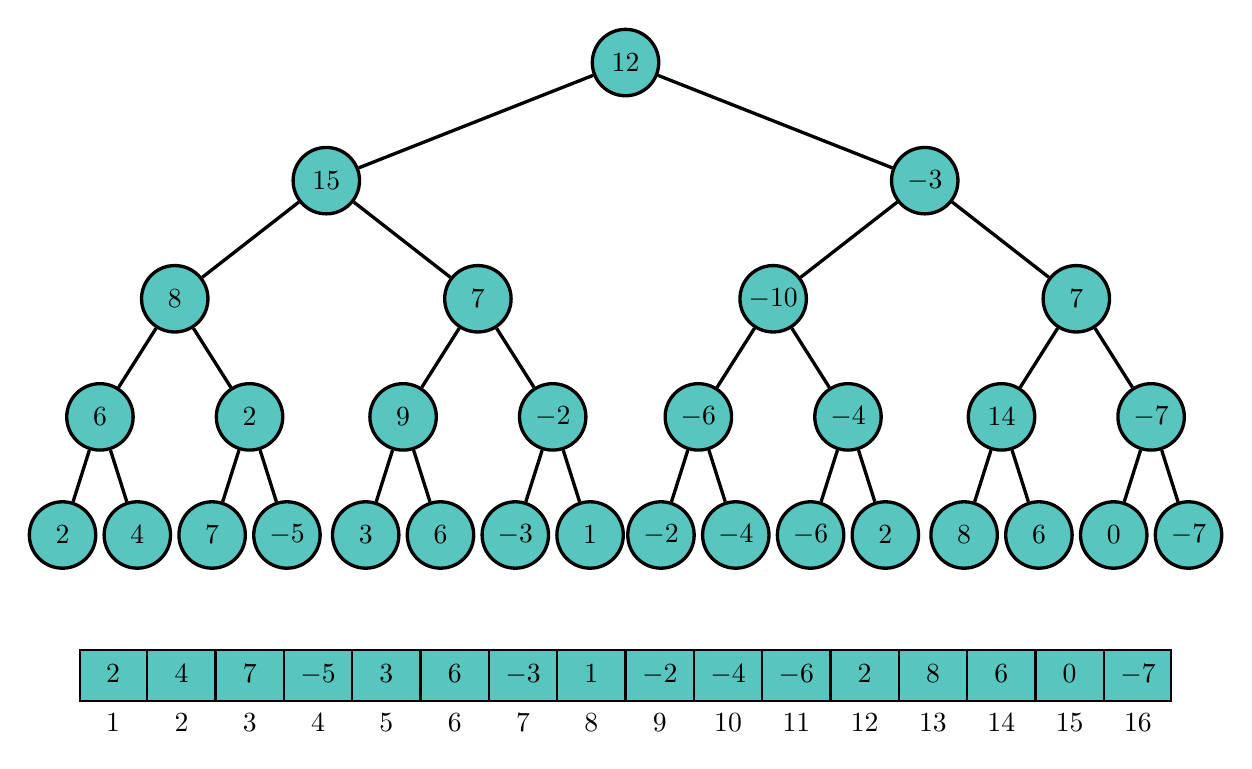
\begin{tikzpicture}[
  very thick,
  level 1/.style={sibling distance=76mm},
  level 2/.style={sibling distance=38.5mm},
  level 3/.style={sibling distance=19mm},
  level 4/.style={sibling distance=9.5mm},
  myrect/.style={
    draw,
    thick,
    fill=myseagreen,
    rectangle split,
    rectangle split horizontal,
    rectangle split parts=#1,
    rectangle split part align=left,
    text width=4ex,
    text centered
    }
]
\node [vertex] (r){$12$}
  child {
    node [vertex] (a) {15}
    child {
      node [vertex] {8}
      child {
        node [vertex] {6}
        child {node [vertex] {2}}
        child {node [vertex] {4}}
      } 
      child {
        node [vertex] {2}
        child {node [vertex] {7}}
        child {node [vertex] {$-5$}}
      }
    }
    child {
      node [vertex] {7}
      child {node [vertex] {9}
              child {node [vertex] {3}}
        child {node [vertex] {6}}
      }
      child {node [vertex] {$-2$}
              child {node [vertex] {$-3$}}
        child {node [vertex] {1}}
      }
    }
  }
  child {
    node [vertex] {$-3$}
    child {
      node [vertex] {$-10$}
      child {node [vertex] {$-6$}
              child {node [vertex] {$-2$}}
        child {node [vertex] {$-4$}}}
      child {node [vertex] {$-4$}
              child {node [vertex] {$-6$}}
        child {node [vertex] {$2$}}}
    }
    child {
      node [vertex] {7}
      child {node [vertex] {14}
              child {node [vertex] {8}}
        child {node [vertex] {6}}}
      child {node [vertex] {$-7$}
              child {node [vertex] {0}}
        child {node [vertex] {$-7$}}}
    }
  };

\node[myrect=16] [below=7cm of r]
  (array)
  {
  					\strut 2
  \nodepart{two}	\strut 4
  \nodepart{three}	\strut 7
  \nodepart{four}	\strut $-5$
  \nodepart{five}	\strut 3
  \nodepart{six}	\strut 6
  \nodepart{seven}	\strut $-3$
  \nodepart{eight}	\strut 1
  \nodepart{nine}	\strut $-2$
  \nodepart{ten}	\strut $-4$
  \nodepart{eleven}	\strut $-6$
  \nodepart{twelve}	\strut 2
  \nodepart{thirteen}	\strut 8
  \nodepart{fourteen}	\strut 6
  \nodepart{fifteen}	\strut 0
  \nodepart{sixteen}	\strut $-7$
  };
\foreach \Valor [count=\Valori from 1] in {one ,two ,three , four , five , six , seven , eight , nine , ten , eleven , twelve , thirteen , fourteen , fifteen , sixteen }
  \node[below] at (array.\Valor south) {\Valori};

\end{tikzpicture}
}
\end{center}

Highlighted are the nodes we'll need to access for $query(7,15)$. Notice how the subtrees associated with each of these nodes neatly covers the entire range $[7,15]$.

\begin{center}
{
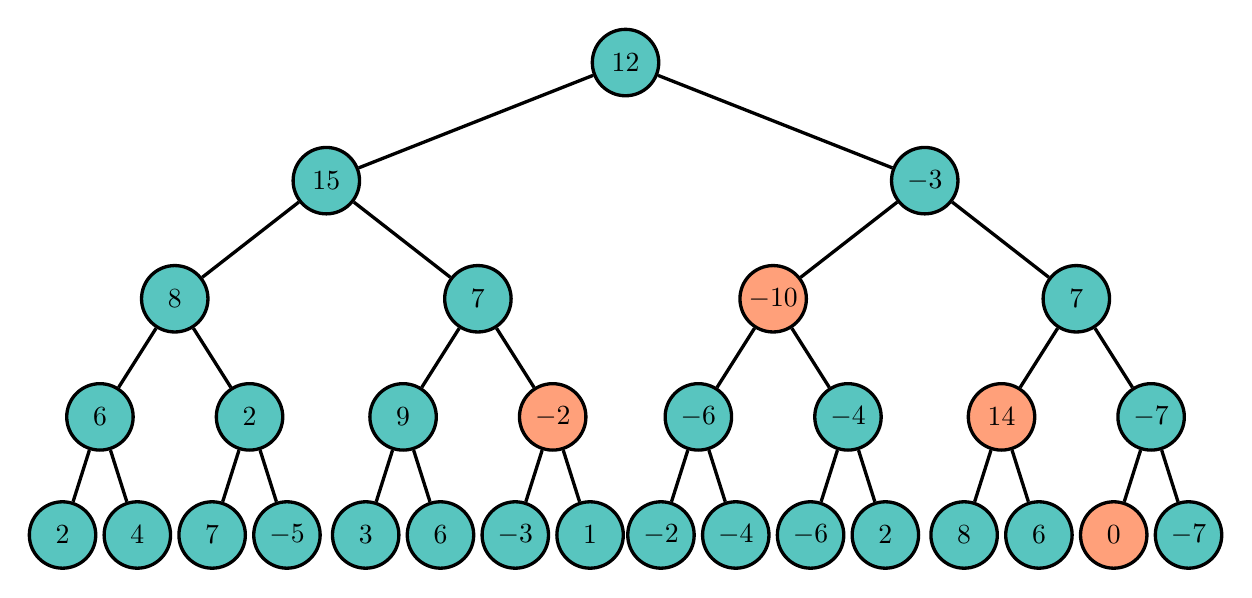
\begin{tikzpicture}[
  very thick,
  level 1/.style={sibling distance=76mm},
  level 2/.style={sibling distance=38.5mm},
  level 3/.style={sibling distance=19mm},
  level 4/.style={sibling distance=9.5mm},
  myrect/.style={
    draw,
    thick,
    fill=myseagreen,
    rectangle split,
    rectangle split horizontal,
    rectangle split parts=#1,
    rectangle split part align=left,
    text width=4ex,
    text centered
    }
]
\node [vertex] (r){$12$}
  child {
    node [vertex] (a) {15}
    child {
      node [vertex] {8}
      child {
        node [vertex] {6}
        child {node [vertex] {2}}
        child {node [vertex] {4}}
      } 
      child {
        node [vertex] {2}
        child {node [vertex] {7}}
        child {node [vertex] {$-5$}}
      }
    }
    child {
      node [vertex] {7}
      child {node [vertex] {9}
              child {node [vertex] {3}}
        child {node [vertex] {6}}
      }
      child {node [vertex, fill=mysalmon] {$-2$}
              child {node [vertex] {$-3$}}
        child {node [vertex] {1}}
      }
    }
  }
  child {
    node [vertex] {$-3$}
    child {
      node [vertex, fill=mysalmon] {$-10$}
      child {node [vertex] {$-6$}
              child {node [vertex] {$-2$}}
        child {node [vertex] {$-4$}}}
      child {node [vertex] {$-4$}
              child {node [vertex] {$-6$}}
        child {node [vertex] {$2$}}}
    }
    child {
      node [vertex] {7}
      child {node [vertex, fill=mysalmon] {14}
              child {node [vertex] {8}}
        child {node [vertex] {6}}}
      child {node [vertex] {$-7$}
              child {node [vertex, fill=mysalmon] {0}}
        child {node [vertex] {$-7$}}}
    }
  };

\end{tikzpicture}
}
\end{center}

Again, the key idea is if the the interval associated with a node is completely contained within the interval we are querying, we simply return the sum associated with that node. Otherwise, we recurse on the two children. This process is $O(\log{n})$ because each level in the tree can have at most two highlighted nodes.

If we wanted to change the third element to 2, we would have to update the highlighted nodes in the following diagram. This process is more straightforward than the querying.

\begin{center}
{
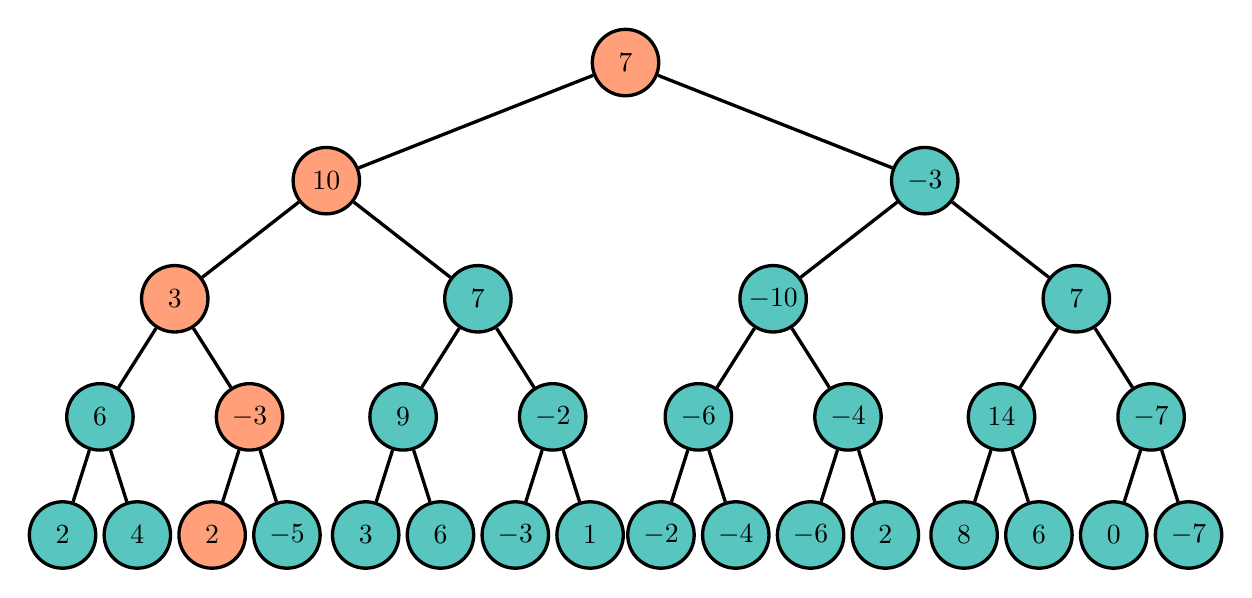
\begin{tikzpicture}[
  very thick,
  level 1/.style={sibling distance=76mm},
  level 2/.style={sibling distance=38.5mm},
  level 3/.style={sibling distance=19mm},
  level 4/.style={sibling distance=9.5mm},
  myrect/.style={
    draw,
    thick,
    fill=myseagreen,
    rectangle split,
    rectangle split horizontal,
    rectangle split parts=#1,
    rectangle split part align=left,
    text width=4ex,
    text centered
    }
]
\node [vertex, fill=mysalmon] (r){7}
  child {
    node [vertex, fill=mysalmon] (a) {10}
    child {
      node [vertex, fill=mysalmon] {3}
      child {
        node [vertex] {6}
        child {node [vertex] {2}}
        child {node [vertex] {4}}
      } 
      child {
        node [vertex, fill=mysalmon] {$-3$}
        child {node [vertex, fill=mysalmon] {2}}
        child {node [vertex] {$-5$}}
      }
    }
    child {
      node [vertex] {7}
      child {node [vertex] {9}
              child {node [vertex] {3}}
        child {node [vertex] {6}}
      }
      child {node [vertex] {$-2$}
              child {node [vertex] {$-3$}}
        child {node [vertex] {1}}
      }
    }
  }
  child {
    node [vertex] {$-3$}
    child {
      node [vertex] {$-10$}
      child {node [vertex] {$-6$}
              child {node [vertex] {$-2$}}
        child {node [vertex] {$-4$}}}
      child {node [vertex] {$-4$}
              child {node [vertex] {$-6$}}
        child {node [vertex] {$2$}}}
    }
    child {
      node [vertex] {7}
      child {node [vertex] {14}
              child {node [vertex] {8}}
        child {node [vertex] {6}}}
      child {node [vertex] {$-7$}
              child {node [vertex] {0}}
        child {node [vertex] {$-7$}}}
    }
  };

\end{tikzpicture}
}
\end{center}

Updating is also $O(\log{n})$ as we need to change the values of at most one node in each level in the tree.

I cheated with my example by using a nice power of two, $n=16$, as the number of elements in the sequence. Of course, the size is not always this nice. One solution is to simply pad the back of the sequence with enough 0s and pretend that the number of elements in the sequence is actually a power of two. For the segment tree, this is not necessary -- if a vertex is associated with the range $[a,b]$, we can simply split this range into two,
$\left[a,\floor{\frac{a+b-1}{2}}\right]$ and $\left[\floor{\frac{a+b-1}{2}}+1,b\right]$. We then recursively apply this pattern except for when the lower bound of the range is equal to the upper bound. If $n=12$, the resulting tree would have the following structure.

\begin{center}
{
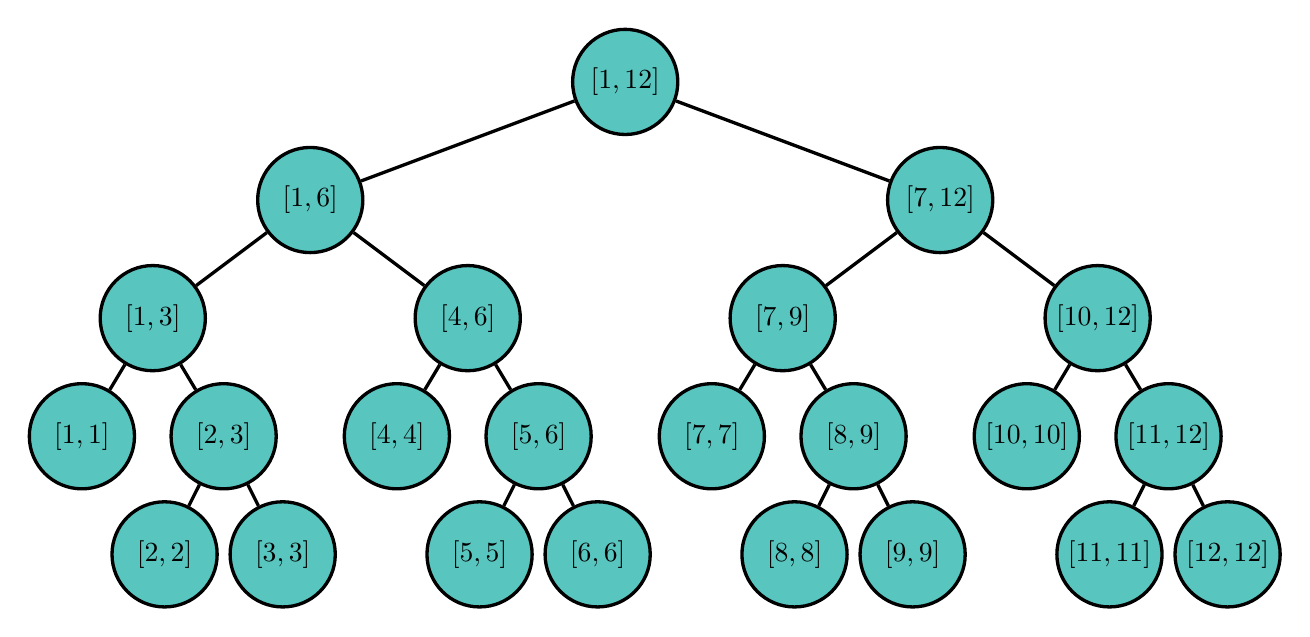
\begin{tikzpicture}[
  very thick,
  level 1/.style={sibling distance=80mm},
  level 2/.style={sibling distance=40mm},
  level 3/.style={sibling distance=18mm},
  level 4/.style={sibling distance=15mm},
]
\node [vertex, minimum size=38pt] (r){$[1,12]$}
  child {
    node [vertex, minimum size=38pt] (a) {$[1,6]$}
    	child {
        	node[vertex, minimum size=38pt] {$[1,3]$}
            	child {
                	node[vertex, minimum size=38pt] {$[1,1]$}
                }
                child {
                	node[vertex, minimum size=38pt] {$[2,3]$}
                    	child {node [vertex, minimum size=38pt] {$[2,2]$}}
                    	child {node [vertex, minimum size=38pt] {$[3,3]$}}
                }
        }
    	child {
        	node[vertex, minimum size=38pt] {$[4,6]$}
            	child {
                	node[vertex, minimum size=38pt] {$[4,4]$}
                }
                child {
                	node[vertex, minimum size=38pt] {$[5,6]$}
                    	child {node [vertex, minimum size=38pt] {$[5,5]$}}
                    	child {node [vertex, minimum size=38pt] {$[6,6]$}}
                }
        }
  }
  child {
    node [vertex, minimum size=38pt] {$[7,12]$}
    	child {
        	node[vertex, minimum size=38pt] {$[7,9]$}
            	child {
                	node[vertex, minimum size=38pt] {$[7,7]$}
                }
                child {
                	node[vertex, minimum size=38pt] {$[8,9]$}
                    	child {node [vertex, minimum size=38pt] {$[8,8]$}}
                    	child {node [vertex, minimum size=38pt] {$[9,9]$}}
                }
        }
    	child {
        	node[vertex, minimum size=38pt] {$[10,12]$}
            	child {
                	node[vertex, minimum size=38pt] {$[10,10]$}
                }
                child {
                	node[vertex, minimum size=38pt] {$[11,12]$}
                    	child {node [vertex, minimum size=38pt] {$[11,11]$}}
                    	child {node [vertex, minimum size=38pt] {$[12,12]$}}
                }
        }
  };

\end{tikzpicture}
}
\end{center}

For this reason, while I used the concept of ``building up'' on top of our array to introduce the segment tree, any operation we implement will start at the root and recursively trickle down the tree. We see that the segment tree structure does not have to resemble a complete tree at all. However, with this approach, it is still quite balanced, so we can store a segment tree within an array as we would a heap.

\subsection{Fenwick Tree}

A \textit{Fenwick tree}, or \textit{binary indexed tree (BIT)}, is simply a faster and easier to code segment tree when the operator in question has an inverse. Unfortunately, it's not at all intuitive, so bear with me at first and let the magic of the Fenwick tree reveal itself later. In fact, it is so magical that Richard Peng hates it because it is too gimmicky. The key idea is to compress the data stored within a segment tree in a crazy way that ends up having a really slick implementation using some bit operation tricks.

As discussed earlier, the $+$ operator has an inverse, $-$. Therefore, there is an inherent redundancy, for example, in keeping track of the sum of the first $\frac{n}{2}$ elements, the sum of all $n$ elements, and the sum of the last $\frac{n}{2}$ elements, as we do in the segment tree. If we are given only $\sum_{k=1}^{n/2} a_k$ and $\sum_{k=1}^n a_k$, we can find $\sum_{k=n/2+1}^{n} a_k$ easily using subtraction.

With this in mind, let's ignore every right child in the tree. We'll mark them as black in the diagram. After that, we'll write out the tree nodes in postfix traversal order, without writing anything whenever we encounter a black node.

\begin{center}
{
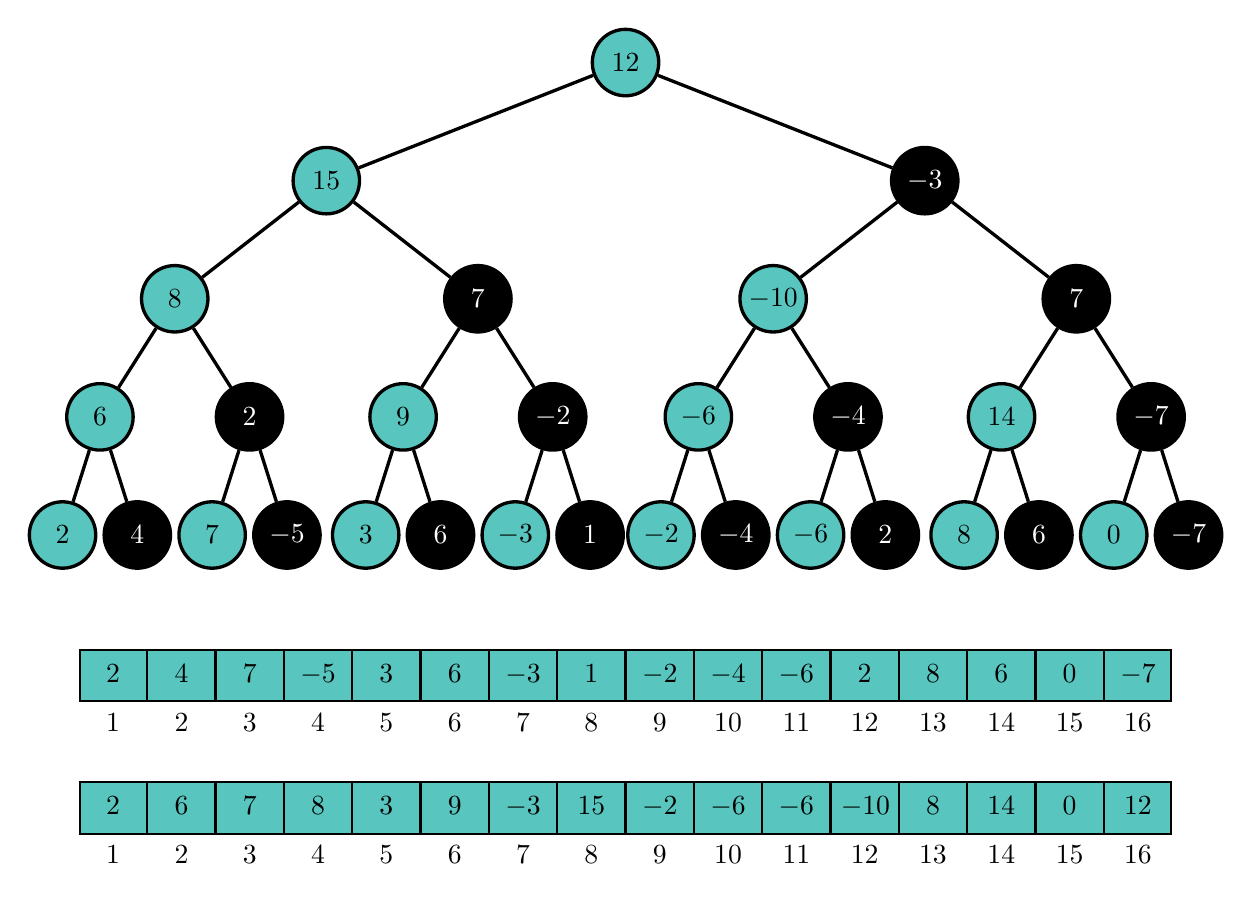
\begin{tikzpicture}[
  very thick,
  level 1/.style={sibling distance=76mm},
  level 2/.style={sibling distance=38.5mm},
  level 3/.style={sibling distance=19mm},
  level 4/.style={sibling distance=9.5mm},
  myrect/.style={
    draw,
    thick,
    fill=myseagreen,
    rectangle split,
    rectangle split horizontal,
    rectangle split parts=#1,
    rectangle split part align=left,
    text width=4ex,
    text centered
    }
]
\node [vertex] (r){$12$}
  child {
    node [vertex] (a) {15}
    child {
      node [vertex] {8}
      child {
        node [vertex] {6}
        child {node [vertex] {2}}
        child {node [vertex, text=mywhite, fill=myblack] {4}}
      } 
      child {
        node [vertex, text=mywhite, fill=myblack] {2}
        child {node [vertex] {7}}
        child {node [vertex, text=mywhite, fill=myblack] {$-5$}}
      }
    }
    child {
      node [vertex, text=mywhite, fill=myblack] {7}
      child {node [vertex] {9}
              child {node [vertex] {3}}
        child {node [vertex, text=mywhite, fill=myblack] {6}}
      }
      child {node [vertex, text=mywhite, fill=myblack] {$-2$}
              child {node [vertex] {$-3$}}
        child {node [vertex, text=mywhite, fill=myblack] {1}}
      }
    }
  }
  child {
    node [vertex, text=mywhite, fill=myblack] {$-3$}
    child {
      node [vertex] {$-10$}
      child {node [vertex] {$-6$}
              child {node [vertex] {$-2$}}
        child {node [vertex, text=mywhite, fill=myblack] {$-4$}}}
      child {node [vertex, text=mywhite, fill=myblack] {$-4$}
              child {node [vertex] {$-6$}}
        child {node [vertex, text=mywhite, fill=myblack] {$2$}}}
    }
    child {
      node [vertex, text=mywhite, fill=myblack] {7}
      child {node [vertex] {14}
              child {node [vertex] {8}}
        child {node [vertex, text=mywhite, fill=myblack] {6}}}
      child {node [vertex, text=mywhite, fill=myblack] {$-7$}
              child {node [vertex] {0}}
        child {node [vertex, text=mywhite, fill=myblack] {$-7$}}}
    }
  };

\node[myrect=16] [below=7cm of r]
  (array)
  {
  					\strut 2
  \nodepart{two}	\strut 4
  \nodepart{three}	\strut 7
  \nodepart{four}	\strut $-5$
  \nodepart{five}	\strut 3
  \nodepart{six}	\strut 6
  \nodepart{seven}	\strut $-3$
  \nodepart{eight}	\strut 1
  \nodepart{nine}	\strut $-2$
  \nodepart{ten}	\strut $-4$
  \nodepart{eleven}	\strut $-6$
  \nodepart{twelve}	\strut 2
  \nodepart{thirteen}	\strut 8
  \nodepart{fourteen}	\strut 6
  \nodepart{fifteen}	\strut 0
  \nodepart{sixteen}	\strut $-7$
  };
\foreach \Valor [count=\Valori from 1] in {one ,two ,three , four , five , six , seven , eight , nine , ten , eleven , twelve , thirteen , fourteen , fifteen , sixteen }
  \node[below] at (array.\Valor south) {\Valori};

\node[myrect=16] [below=of array]
  (array2)
  {
  					\strut 2
  \nodepart{two}	\strut 6
  \nodepart{three}	\strut 7
  \nodepart{four}	\strut 8
  \nodepart{five}	\strut 3
  \nodepart{six}	\strut 9
  \nodepart{seven}	\strut $-3$
  \nodepart{eight}	\strut 15
  \nodepart{nine}	\strut $-2$
  \nodepart{ten}	\strut $-6$
  \nodepart{eleven}	\strut $-6$
  \nodepart{twelve}	\strut $-10$
  \nodepart{thirteen}	\strut 8
  \nodepart{fourteen}	\strut 14
  \nodepart{fifteen}	\strut 0
  \nodepart{sixteen}	\strut 12
  };
\foreach \Valor [count=\Valori from 1] in {one ,two ,three , four , five , six , seven , eight , nine , ten , eleven , twelve , thirteen , fourteen , fifteen , sixteen }
  \node[below] at (array2.\Valor south) {\Valori};

\end{tikzpicture}
}
\end{center}

Our Fenwick tree is simply this last array. This should be quite confusing -- it is not at all clear why this array resembles a tree, and the numbers in the array make no sense whatsoever right now.

Notice that the final position of every unblackened node is just the rightmost black child in its subtree. This leads to the fact that the $i$th element in the Fenwick tree array is the sum

\[b_k = \sum_{k=i-2^{v_2(i)}+1}^i a_k, \]

where $2^{v_2(i)}$ is simply the greatest power of 2 that divides $i$. Let's look at a new diagram that hopefully will better illustrate this key property of the random array we just came up with.

\begin{center}
{
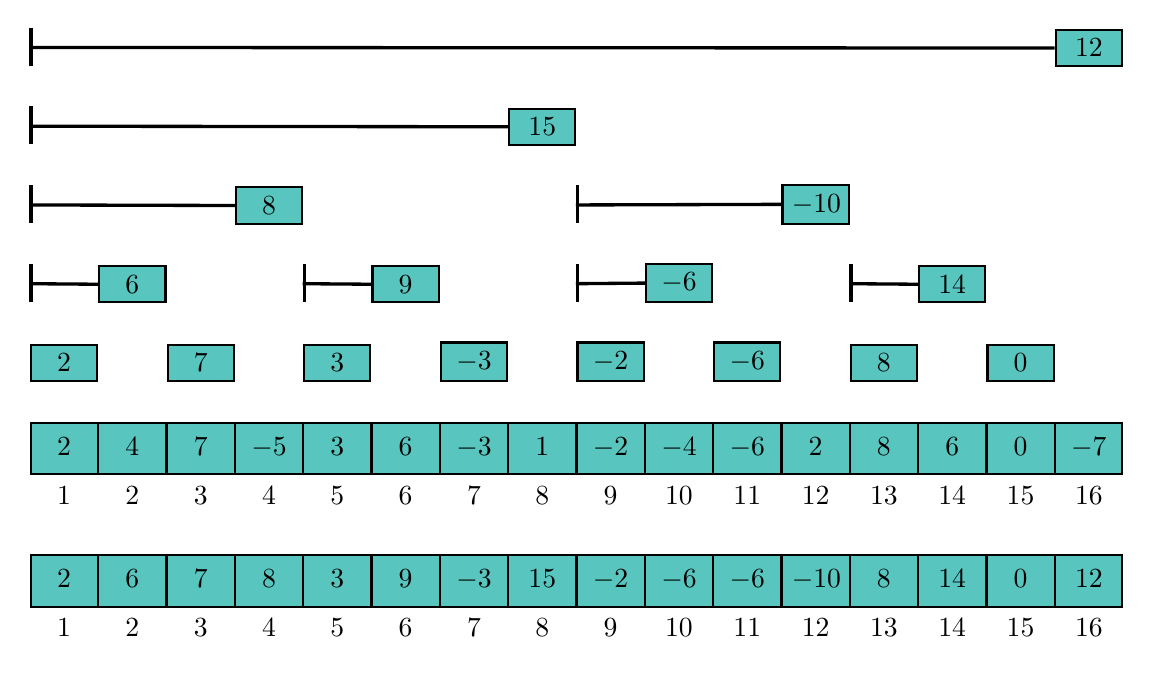
\begin{tikzpicture}[
  very thick,
  myrect/.style={
    draw,
    thick,
    fill=myseagreen,
    rectangle split,
    rectangle split horizontal,
    rectangle split parts=#1,
    rectangle split part align=left,
    text width=4ex,
    text centered
    },
  onesided/.style={
        text width=4ex,
        draw=none,
        append after command={
            [shorten <= -0.5\pgflinewidth] 
            ([shift={( 0.5\pgflinewidth,-0.5\pgflinewidth)}]\tikzlastnode.north west)
        edge([shift={( 0.5\pgflinewidth,+0.5\pgflinewidth)}]\tikzlastnode.south west)            
        }
    }
]

\node[myrect=16]
  (array)
  {
  					\strut 2
  \nodepart{two}	\strut 4
  \nodepart{three}	\strut 7
  \nodepart{four}	\strut $-5$
  \nodepart{five}	\strut 3
  \nodepart{six}	\strut 6
  \nodepart{seven}	\strut $-3$
  \nodepart{eight}	\strut 1
  \nodepart{nine}	\strut $-2$
  \nodepart{ten}	\strut $-4$
  \nodepart{eleven}	\strut $-6$
  \nodepart{twelve}	\strut 2
  \nodepart{thirteen}	\strut 8
  \nodepart{fourteen}	\strut 6
  \nodepart{fifteen}	\strut 0
  \nodepart{sixteen}	\strut $-7$
  };
\foreach \Valor [count=\Valori from 1] in {one ,two ,three , four , five , six , seven , eight , nine , ten , eleven , twelve , thirteen , fourteen , fifteen , sixteen }
  \node[below] at (array.\Valor south) {\Valori};

\node[myrect=1, above=5mm] at (array.one north) (n1) {2};
\node[myrect=1, above=15mm] at (array.two north) (n2) {6};
\node[myrect=1, above=5mm] at (array.three north) (n3) {7};
\node[myrect=1, above=25mm] at (array.four north) (n4) {8};
\node[myrect=1, above=5mm] at (array.five north) (n5) {3};
\node[myrect=1, above=15mm] at (array.six north) (n6) {9};
\node[myrect=1, above=5mm] at (array.seven north) (n7) {$-3$};
\node[myrect=1, above=35mm] at (array.eight north) (n8) {15};
\node[myrect=1, above=5mm] at (array.nine north) (n9) {$-2$};
\node[myrect=1, above=15mm] at (array.ten north) (n10) {$-6$};
\node[myrect=1, above=5mm] at (array.eleven north) (n11) {$-6$};
\node[myrect=1, above=25mm] at (array.twelve north) (n12) {$-10$};
\node[myrect=1, above=5mm] at (array.thirteen north) (n13) {8};
\node[myrect=1, above=15mm] at (array.fourteen north) (n14) {14};
\node[myrect=1, above=5mm] at (array.fifteen north) (n15) {0};
\node[myrect=1, above=45mm] at (array.sixteen north) (n16) {12};

\node[onesided, above=15mm] at (array.one north) (m2) { \phantom{0} };
\node[onesided, above=25mm] at (array.one north) (m4) { \phantom{0} };
\node[onesided, above=15mm] at (array.five north) (m6) { \phantom{0} };
\node[onesided, above=35mm] at (array.one north) (m8) { \phantom{0} };
\node[onesided, above=15mm] at (array.nine north) (m10) { \phantom{0} };
\node[onesided, above=25mm] at (array.nine north) (m12) { \phantom{0} };
\node[onesided, above=15mm] at (array.thirteen north) (m14) { \phantom{0} };
\node[onesided, above=45mm] at (array.one north) (m16) { \phantom{0} };

\draw (m2.west) -- (n2.west);
\draw (m4.west) -- (n4.west);
\draw (m6.west) -- (n6.west);
\draw (m8.west) -- (n8.west);
\draw (m10.west) -- (n10.west);
\draw (m12.west) -- (n12.west);
\draw (m14.west) -- (n14.west);
\draw (m16.west) -- (n16.west);

\node[myrect=16] [below=of array]
  (array2)
  {
  					\strut 2
  \nodepart{two}	\strut 6
  \nodepart{three}	\strut 7
  \nodepart{four}	\strut 8
  \nodepart{five}	\strut 3
  \nodepart{six}	\strut 9
  \nodepart{seven}	\strut $-3$
  \nodepart{eight}	\strut 15
  \nodepart{nine}	\strut $-2$
  \nodepart{ten}	\strut $-6$
  \nodepart{eleven}	\strut $-6$
  \nodepart{twelve}	\strut $-10$
  \nodepart{thirteen}	\strut 8
  \nodepart{fourteen}	\strut 14
  \nodepart{fifteen}	\strut 0
  \nodepart{sixteen}	\strut 12
  };
\foreach \Valor [count=\Valori from 1] in {one ,two ,three , four , five , six , seven , eight , nine , ten , eleven , twelve , thirteen , fourteen , fifteen , sixteen }
  \node[below] at (array2.\Valor south) {\Valori};

\end{tikzpicture}
}
\end{center}

All the framework is now in place. Now we need to find out how to query and update the Fenwick tree.

Suppose we wanted to find the sum $\sum_{k=1}^{11} a_k$. Let's take a look at the diagram to see which elements we need.

\begin{center}
{
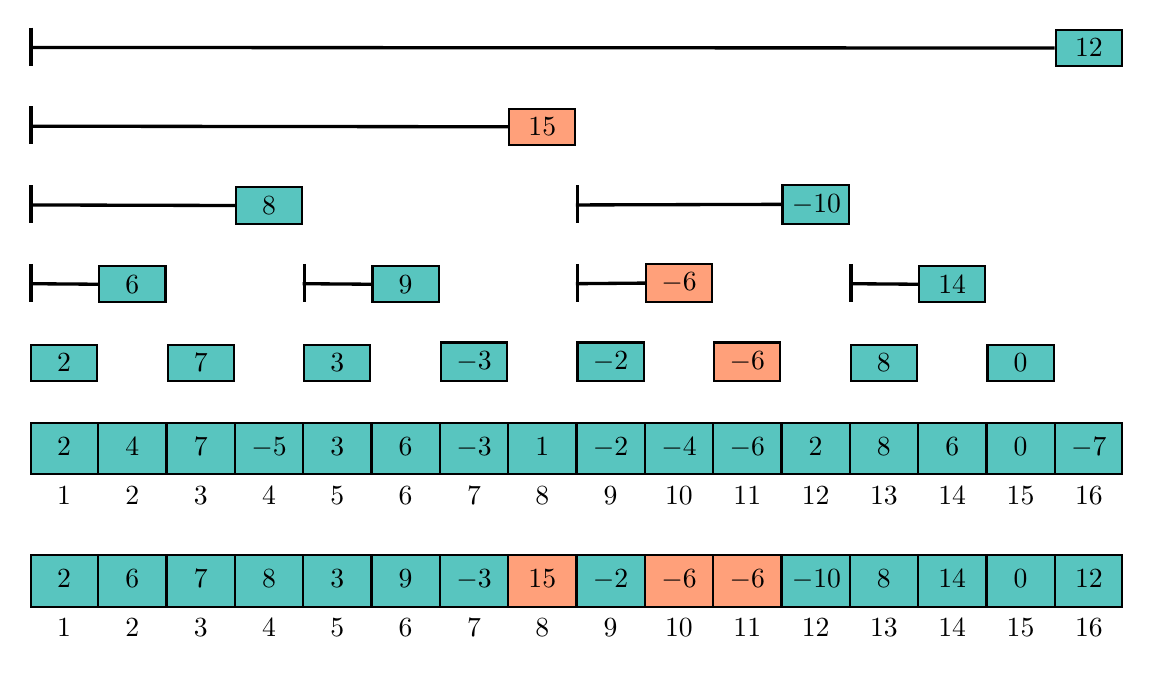
\begin{tikzpicture}[
  very thick,
  myrect2/.style={
    draw,
    thick,
    rectangle split,
    rectangle split horizontal,
    rectangle split parts=#1,
    rectangle split part align=left,
    text width=4ex,
    text centered
    },
  myrect/.style={
    draw,
    thick,
    rectangle split,
    rectangle split horizontal,
    rectangle split parts=#1,
    fill=myseagreen,
    rectangle split part align=left,
    text width=4ex,
    text centered,
  	fill=myseagreen
  },
  onesided/.style={
        text width=4ex,
        draw=none,
        append after command={
            [shorten <= -0.5\pgflinewidth] 
            ([shift={( 0.5\pgflinewidth,-0.5\pgflinewidth)}]\tikzlastnode.north west)
        edge([shift={( 0.5\pgflinewidth,+0.5\pgflinewidth)}]\tikzlastnode.south west)            
        }
    }
]

\node[myrect=16]
  (array)
  {
  					\strut 2
  \nodepart{two}	\strut 4
  \nodepart{three}	\strut 7
  \nodepart{four}	\strut $-5$
  \nodepart{five}	\strut 3
  \nodepart{six}	\strut 6
  \nodepart{seven}	\strut $-3$
  \nodepart{eight}	\strut 1
  \nodepart{nine}	\strut $-2$
  \nodepart{ten}	\strut $-4$
  \nodepart{eleven}	\strut $-6$
  \nodepart{twelve}	\strut 2
  \nodepart{thirteen}	\strut 8
  \nodepart{fourteen}	\strut 6
  \nodepart{fifteen}	\strut 0
  \nodepart{sixteen}	\strut $-7$
  };
\foreach \Valor [count=\Valori from 1] in {one ,two ,three , four , five , six , seven , eight , nine , ten , eleven , twelve , thirteen , fourteen , fifteen , sixteen }
  \node[below] at (array.\Valor south) {\Valori};

\node[myrect=1, above=5mm] at (array.one north) (n1) {2};
\node[myrect=1, above=15mm] at (array.two north) (n2) {6};
\node[myrect=1, above=5mm] at (array.three north) (n3) {7};
\node[myrect=1, above=25mm] at (array.four north) (n4) {8};
\node[myrect=1, above=5mm] at (array.five north) (n5) {3};
\node[myrect=1, above=15mm] at (array.six north) (n6) {9};
\node[myrect=1, above=5mm] at (array.seven north) (n7) {$-3$};
\node[myrect=1, above=35mm, fill=mysalmon] at (array.eight north) (n8) {15};
\node[myrect=1, above=5mm] at (array.nine north) (n9) {$-2$};
\node[myrect=1, above=15mm, fill=mysalmon] at (array.ten north) (n10) {$-6$};
\node[myrect=1, above=5mm, fill=mysalmon] at (array.eleven north) (n11) {$-6$};
\node[myrect=1, above=25mm] at (array.twelve north) (n12) {$-10$};
\node[myrect=1, above=5mm] at (array.thirteen north) (n13) {8};
\node[myrect=1, above=15mm] at (array.fourteen north) (n14) {14};
\node[myrect=1, above=5mm] at (array.fifteen north) (n15) {0};
\node[myrect=1, above=45mm] at (array.sixteen north) (n16) {12};

\node[onesided, above=15mm] at (array.one north) (m2) { \phantom{0} };
\node[onesided, above=25mm] at (array.one north) (m4) { \phantom{0} };
\node[onesided, above=15mm] at (array.five north) (m6) { \phantom{0} };
\node[onesided, above=35mm] at (array.one north) (m8) { \phantom{0} };
\node[onesided, above=15mm] at (array.nine north) (m10) { \phantom{0} };
\node[onesided, above=25mm] at (array.nine north) (m12) { \phantom{0} };
\node[onesided, above=15mm] at (array.thirteen north) (m14) { \phantom{0} };
\node[onesided, above=45mm] at (array.one north) (m16) { \phantom{0} };

\draw (m2.west) -- (n2.west);
\draw (m4.west) -- (n4.west);
\draw (m6.west) -- (n6.west);
\draw (m8.west) -- (n8.west);
\draw (m10.west) -- (n10.west);
\draw (m12.west) -- (n12.west);
\draw (m14.west) -- (n14.west);
\draw (m16.west) -- (n16.west);

\node[myrect2=16, rectangle split part fill={myseagreen, myseagreen, myseagreen, myseagreen, myseagreen, myseagreen, myseagreen, mysalmon, myseagreen, mysalmon, mysalmon, myseagreen, myseagreen, myseagreen, myseagreen, myseagreen}] [below=of array]
  (array2)
  {
  					\strut 2
  \nodepart{two}	\strut 6
  \nodepart{three}	\strut 7
  \nodepart{four}	\strut 8
  \nodepart{five}	\strut 3
  \nodepart{six}	\strut 9
  \nodepart{seven}	\strut $-3$
  \nodepart{eight}	\strut 15
  \nodepart{nine}	\strut $-2$
  \nodepart{ten}	\strut $-6$
  \nodepart{eleven}	\strut $-6$
  \nodepart{twelve}	\strut $-10$
  \nodepart{thirteen}	\strut 8
  \nodepart{fourteen}	\strut 14
  \nodepart{fifteen}	\strut 0
  \nodepart{sixteen}	\strut 12
  };
\foreach \Valor [count=\Valori from 1] in {one ,two ,three , four , five , six , seven , eight , nine , ten , eleven , twelve , thirteen , fourteen , fifteen , sixteen }
  \node[below] at (array2.\Valor south) {\Valori};

\end{tikzpicture}
}
\end{center}

We see that the sum $\sum_{k=1}^{11}a_k=b_8+b_{10}+b_{11}$. If we look at 11 in binary, we have $11=01011_2$. Let's see if we can find a pattern in these numbers in binary:

\begin{align*}
11 &= 01011_2, \\
10 = 11-2^{v_2(11)} &= 01010_2, \\
8 = 10-2^{v_2(10)} &= 01000_2, \\
0=8-2^{v_2(8)}&=00000_2.
\end{align*}

So, we can simply subtract $11-2^{v_2(11)}=10=01010_2$, find the sum of the first 10 elements, and add $b_{11}$ to that sum to get the sum of the first 11 elements. We see that repeating this process takes off the last 1 in the binary representation of the number $i$, and since there are at most $\log{n}+1$ 1s in the binary representation $\forall i \in [1,n]$, the query operation is $O(\log{n})$.

And now for the update operation. Suppose we want to change the value of $a_{11}$ from $-6$ to $-3$. Which numbers will we have to change?

\begin{center}
{
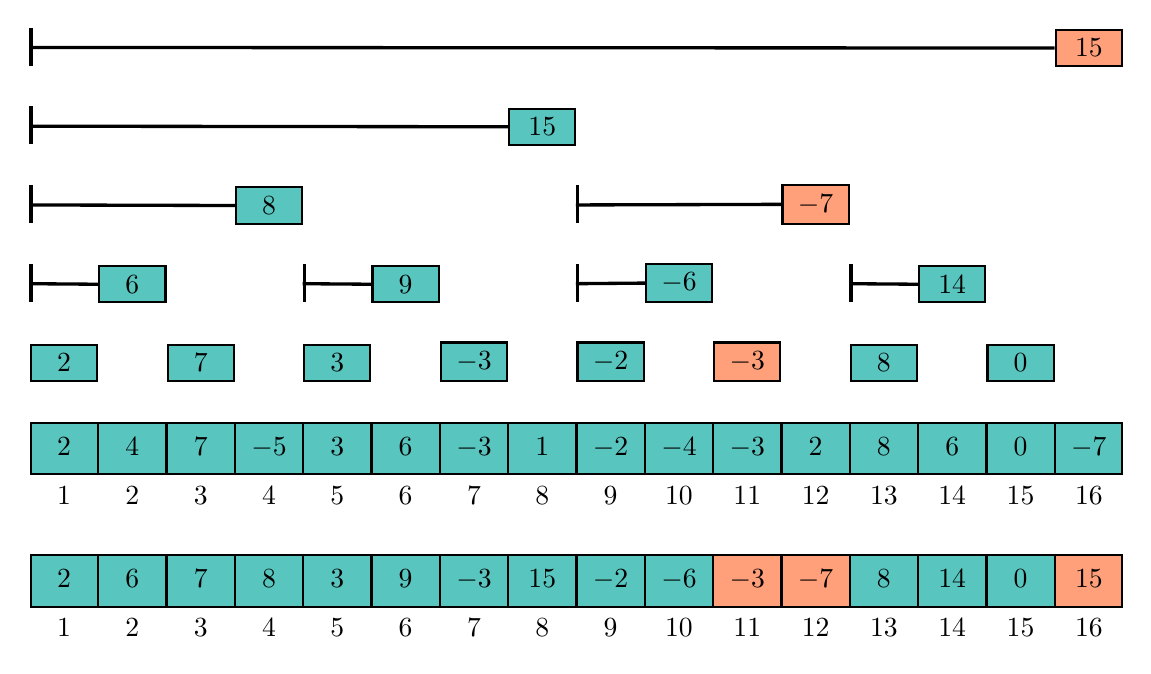
\begin{tikzpicture}[
  very thick,
  myrect2/.style={
    draw,
    thick,
    rectangle split,
    rectangle split horizontal,
    rectangle split parts=#1,
    rectangle split part align=left,
    text width=4ex,
    text centered
    },
  myrect/.style={
    draw,
    thick,
    rectangle split,
    rectangle split horizontal,
    rectangle split parts=#1,
    fill=myseagreen,
    rectangle split part align=left,
    text width=4ex,
    text centered,
  	fill=myseagreen
  },
  onesided/.style={
        text width=4ex,
        draw=none,
        append after command={
            [shorten <= -0.5\pgflinewidth] 
            ([shift={( 0.5\pgflinewidth,-0.5\pgflinewidth)}]\tikzlastnode.north west)
        edge([shift={( 0.5\pgflinewidth,+0.5\pgflinewidth)}]\tikzlastnode.south west)            
        }
    }
]

\node[myrect=16]
  (array)
  {
  					\strut 2
  \nodepart{two}	\strut 4
  \nodepart{three}	\strut 7
  \nodepart{four}	\strut $-5$
  \nodepart{five}	\strut 3
  \nodepart{six}	\strut 6
  \nodepart{seven}	\strut $-3$
  \nodepart{eight}	\strut 1
  \nodepart{nine}	\strut $-2$
  \nodepart{ten}	\strut $-4$
  \nodepart{eleven}	\strut $-3$
  \nodepart{twelve}	\strut 2
  \nodepart{thirteen}	\strut 8
  \nodepart{fourteen}	\strut 6
  \nodepart{fifteen}	\strut 0
  \nodepart{sixteen}	\strut $-7$
  };
\foreach \Valor [count=\Valori from 1] in {one ,two ,three , four , five , six , seven , eight , nine , ten , eleven , twelve , thirteen , fourteen , fifteen , sixteen }
  \node[below] at (array.\Valor south) {\Valori};

\node[myrect=1, above=5mm] at (array.one north) (n1) {2};
\node[myrect=1, above=15mm] at (array.two north) (n2) {6};
\node[myrect=1, above=5mm] at (array.three north) (n3) {7};
\node[myrect=1, above=25mm] at (array.four north) (n4) {8};
\node[myrect=1, above=5mm] at (array.five north) (n5) {3};
\node[myrect=1, above=15mm] at (array.six north) (n6) {9};
\node[myrect=1, above=5mm] at (array.seven north) (n7) {$-3$};
\node[myrect=1, above=35mm] at (array.eight north) (n8) {15};
\node[myrect=1, above=5mm] at (array.nine north) (n9) {$-2$};
\node[myrect=1, above=15mm] at (array.ten north) (n10) {$-6$};
\node[myrect=1, above=5mm, fill=mysalmon] at (array.eleven north) (n11) {$-3$};
\node[myrect=1, above=25mm, fill=mysalmon] at (array.twelve north) (n12) {$-7$};
\node[myrect=1, above=5mm] at (array.thirteen north) (n13) {8};
\node[myrect=1, above=15mm] at (array.fourteen north) (n14) {14};
\node[myrect=1, above=5mm] at (array.fifteen north) (n15) {0};
\node[myrect=1, above=45mm, fill=mysalmon] at (array.sixteen north) (n16) {15};

\node[onesided, above=15mm] at (array.one north) (m2) { \phantom{0} };
\node[onesided, above=25mm] at (array.one north) (m4) { \phantom{0} };
\node[onesided, above=15mm] at (array.five north) (m6) { \phantom{0} };
\node[onesided, above=35mm] at (array.one north) (m8) { \phantom{0} };
\node[onesided, above=15mm] at (array.nine north) (m10) { \phantom{0} };
\node[onesided, above=25mm] at (array.nine north) (m12) { \phantom{0} };
\node[onesided, above=15mm] at (array.thirteen north) (m14) { \phantom{0} };
\node[onesided, above=45mm] at (array.one north) (m16) { \phantom{0} };

\draw (m2.west) -- (n2.west);
\draw (m4.west) -- (n4.west);
\draw (m6.west) -- (n6.west);
\draw (m8.west) -- (n8.west);
\draw (m10.west) -- (n10.west);
\draw (m12.west) -- (n12.west);
\draw (m14.west) -- (n14.west);
\draw (m16.west) -- (n16.west);

\node[myrect2=16, rectangle split part fill={myseagreen, myseagreen, myseagreen, myseagreen, myseagreen, myseagreen, myseagreen, myseagreen, myseagreen, myseagreen, mysalmon, mysalmon, myseagreen, myseagreen, myseagreen, mysalmon}] [below=of array]
  (array2)
  {
  					\strut 2
  \nodepart{two}	\strut 6
  \nodepart{three}	\strut 7
  \nodepart{four}	\strut 8
  \nodepart{five}	\strut 3
  \nodepart{six}	\strut 9
  \nodepart{seven}	\strut $-3$
  \nodepart{eight}	\strut 15
  \nodepart{nine}	\strut $-2$
  \nodepart{ten}	\strut $-6$
  \nodepart{eleven}	\strut $-3$
  \nodepart{twelve}	\strut $-7$
  \nodepart{thirteen}	\strut 8
  \nodepart{fourteen}	\strut 14
  \nodepart{fifteen}	\strut 0
  \nodepart{sixteen}	\strut 15
  };
\foreach \Valor [count=\Valori from 1] in {one ,two ,three , four , five , six , seven , eight , nine , ten , eleven , twelve , thirteen , fourteen , fifteen , sixteen }
  \node[below] at (array2.\Valor south) {\Valori};

\end{tikzpicture}
}
\end{center}

We needed to increment the highlighted values, $b_{11}$, $b_{12}$, and $b_{16}$, by 3. Once again we'll look at 11, 12, and 16 in base 2.

\begin{align*}
11 &= 01011_2, \\
12 &= 01100_2 = 11 + 2^{v_2(11)}, \\
16 &= 10000_2 = 12 + 2^{v_2(12)}.
\end{align*}

It appears that instead of subtracting the largest dividing power of 2, we are adding. Once again this is an $O(\log{n})$ operation.

The real magic in the Fenwick tree is how quickly it can be coded. The only tricky part is finding exactly what $2^{v_2(i)}$ is. But it turns out, by the way bits are arranged in negative numbers, this is just \texttt{i \& -i}. With this in mind, here's all the code that's necessary to code a Fenwick tree.

\begin{mylstlisting}
int[] b = new int[MAXN]; // Fenwick tree stored as array
void update(int i, int x) {
	for( ; i < MAXN; i += i & -i)
		b[i] += x;
}
int prefixSum(int i) {
	int sum = 0;
	for( ; i > 0; i -= i & -i)
		sum += b[i];
	return sum;
}
int query(int i, int j) {
	return prefixSum(j) - prefixSum(i - 1);
}
\end{mylstlisting}

\subsection{Lazy Propagation}

It is often the case that in addition to performing range queries, we need to be able to perform \textit{range updates}. (Before, we only had to implement point updates.) One extension of our sum problem would require the following two functions:

\begin{itemize}
\item
$update(i, j, x)$ -- increment the value of $a_k$ by $x$ for all $k\in [i,j]$

\item
$query(i, j)$ -- return $\sum_{k=i}^j a_k$.
\end{itemize}

\subsubsection{Some Motivation: $\sqrt{n}$ Blocking}

Let's go back to our $\sqrt{n}$ blocking solution and see what changes we can make, and hopefully we can extend this idea back to our segment tree. If we're looking for an $O(\sqrt{n})$ implementation for $update$, we clearly can't perform point updates for all values in the range. The way we sped up $query$ was by keeping track of an extra set of data, the sum of all the elements in a bucket, which we used when \textit{the entire bucket was in the query range}.

\begin{center}
{
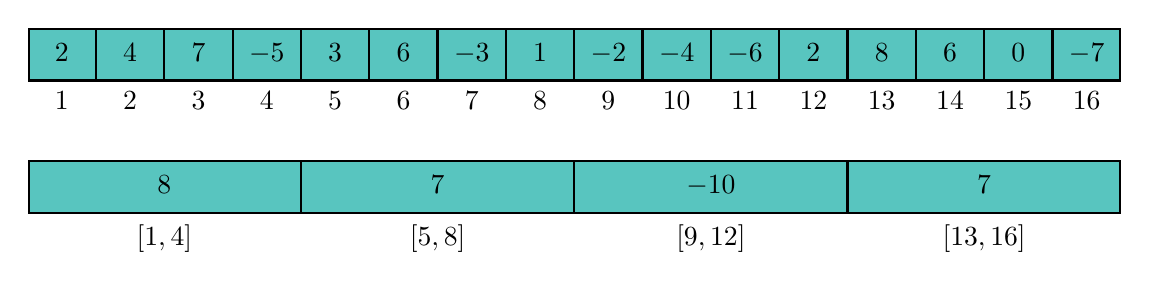
\begin{tikzpicture}[
  thick,
  myrect/.style={
    draw,
    fill=myseagreen,
    rectangle split,
    rectangle split horizontal,
    rectangle split parts=#1,
    rectangle split part align=left,
    text width=4ex,
    text centered
    }
]

\node[myrect=16]
  (array2)
  {
  					\strut 2
  \nodepart{two}	\strut 4
  \nodepart{three}	\strut 7
  \nodepart{four}	\strut $-5$
  \nodepart{five}	\strut 3
  \nodepart{six}	\strut 6
  \nodepart{seven}	\strut $-3$
  \nodepart{eight}	\strut 1
  \nodepart{nine}	\strut $-2$
  \nodepart{ten}	\strut $-4$
  \nodepart{eleven}	\strut $-6$
  \nodepart{twelve}	\strut 2
  \nodepart{thirteen}	\strut 8
  \nodepart{fourteen}	\strut 6
  \nodepart{fifteen}	\strut 0
  \nodepart{sixteen}	\strut $-7$
  };
\foreach \Valor [count=\Valori from 1] in {one ,two ,three , four , five , six , seven , eight , nine , ten , eleven , twelve , thirteen , fourteen , fifteen , sixteen }
  \node[below] at (array2.\Valor south) {\Valori};

\node[myrect=4, text width=21.2ex] [below=of array2]
  (array)
  {
  					\strut 8
  \nodepart{two}	\strut 7
  \nodepart{three}	\strut $-10$
  \nodepart{four}	\strut 7
  };

\node[below] at (array.one south) {$[1,4]$};
\node[below] at (array.two south) {$[5,8]$};
\node[below] at (array.three south) {$[9,12]$};
\node[below] at (array.four south) {$[13,16]$};
\end{tikzpicture}
}
\end{center}

What can we do with this idea for $update$? Let's see what we can do if an entire bucket were included in the update range. Again, we don't want to touch the original array $a$ at all since that makes the operation linear. Let's try storing some information separately. This other information we're storing is the key idea behind lazy propagation.

With this in mind, highlighted are the elements we'll need for $update(4,14,3)$.

\begin{center}
{
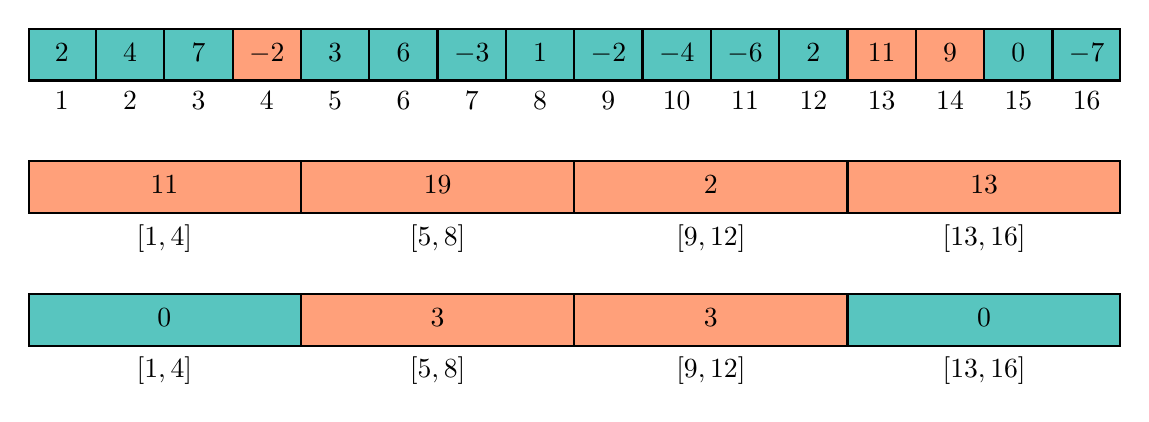
\begin{tikzpicture}[
  thick,
  myrect/.style={
    draw,
    rectangle split,
    rectangle split horizontal,
    rectangle split parts=#1,
    rectangle split part align=left,
    text width=4ex,
    text centered
    }
]

\node[myrect=16, rectangle split part fill={myseagreen, myseagreen, myseagreen, mysalmon, myseagreen, myseagreen, myseagreen, myseagreen, myseagreen, myseagreen, myseagreen, myseagreen, mysalmon, mysalmon, myseagreen, myseagreen}]
  (array2)
  {
  					\strut 2
  \nodepart{two}	\strut 4
  \nodepart{three}	\strut 7
  \nodepart{four}	\strut $-2$
  \nodepart{five}	\strut 3
  \nodepart{six}	\strut 6
  \nodepart{seven}	\strut $-3$
  \nodepart{eight}	\strut 1
  \nodepart{nine}	\strut $-2$
  \nodepart{ten}	\strut $-4$
  \nodepart{eleven}	\strut $-6$
  \nodepart{twelve}	\strut 2
  \nodepart{thirteen}	\strut 11
  \nodepart{fourteen}	\strut 9
  \nodepart{fifteen}	\strut 0
  \nodepart{sixteen}	\strut $-7$
  };
\foreach \Valor [count=\Valori from 1] in {one ,two ,three , four , five , six , seven , eight , nine , ten , eleven , twelve , thirteen , fourteen , fifteen , sixteen }
  \node[below] at (array2.\Valor south) {\Valori};

\node[myrect=4, text width=21.2ex, rectangle split part fill={mysalmon, mysalmon, mysalmon, mysalmon}] [below=of array2]
  (array)
  {
  					\strut 11
  \nodepart{two}	\strut 19
  \nodepart{three}	\strut 2
  \nodepart{four}	\strut 13
  };

\node[below] at (array.one south) {$[1,4]$};
\node[below] at (array.two south) {$[5,8]$};
\node[below] at (array.three south) {$[9,12]$};
\node[below] at (array.four south) {$[13,16]$};

\node[myrect=4, text width=21.2ex, rectangle split part fill={myseagreen, mysalmon, mysalmon, myseagreen}] [below=of array]
  (array3)
  {
  					\strut 0
  \nodepart{two}	\strut 3
  \nodepart{three}	\strut 3
  \nodepart{four}	\strut 0
  };

\node[below] at (array3.one south) {$[1,4]$};
\node[below] at (array3.two south) {$[5,8]$};
\node[below] at (array3.three south) {$[9,12]$};
\node[below] at (array3.four south) {$[13,16]$};
\end{tikzpicture}
}
\end{center}

Note that the sums associated with each bucket must adjust appropriately. In the example, there are four elements per bucket, so when an entire bucket needs to be incremented by 3, a single bucket can increment its sum by $4 \cdot 3 = 12$ easily.

To reiterate, we not storing the actual values of the elements where they were stored in solving the original formulation of the problem. Despite this fact, we are able to calculate what any single value is supposed to be. $a_i$ is simply equal to the $\ceiling{\frac{i}{\sqrt{n}}}$th value stored in the newest third array added to the $i$th value stored in the first array. Because of this, querying a range works in almost exactly the same way as it did in the original formulation.

Highlighted are the values necessary for $query(7,15)$.

\begin{center}
{
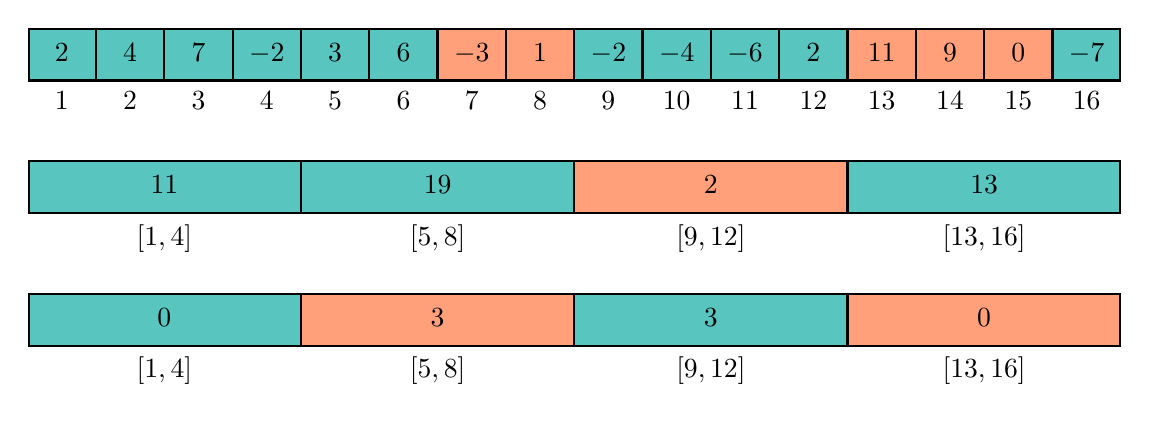
\begin{tikzpicture}[
  thick,
  myrect/.style={
    draw,
    rectangle split,
    rectangle split horizontal,
    rectangle split parts=#1,
    rectangle split part align=left,
    text width=4ex,
    text centered
    }
]

\node[myrect=16, rectangle split part fill={myseagreen, myseagreen, myseagreen, myseagreen, myseagreen, myseagreen, mysalmon, mysalmon, myseagreen, myseagreen, myseagreen, myseagreen, mysalmon, mysalmon, mysalmon, myseagreen}]
  (array2)
  {
  					\strut 2
  \nodepart{two}	\strut 4
  \nodepart{three}	\strut 7
  \nodepart{four}	\strut $-2$
  \nodepart{five}	\strut 3
  \nodepart{six}	\strut 6
  \nodepart{seven}	\strut $-3$
  \nodepart{eight}	\strut 1
  \nodepart{nine}	\strut $-2$
  \nodepart{ten}	\strut $-4$
  \nodepart{eleven}	\strut $-6$
  \nodepart{twelve}	\strut 2
  \nodepart{thirteen}	\strut 11
  \nodepart{fourteen}	\strut 9
  \nodepart{fifteen}	\strut 0
  \nodepart{sixteen}	\strut $-7$
  };
\foreach \Valor [count=\Valori from 1] in {one ,two ,three , four , five , six , seven , eight , nine , ten , eleven , twelve , thirteen , fourteen , fifteen , sixteen }
  \node[below] at (array2.\Valor south) {\Valori};

\node[myrect=4, text width=21.2ex, rectangle split part fill={myseagreen, myseagreen, mysalmon, myseagreen}] [below=of array2]
  (array)
  {
  					\strut 11
  \nodepart{two}	\strut 19
  \nodepart{three}	\strut 2
  \nodepart{four}	\strut 13
  };

\node[below] at (array.one south) {$[1,4]$};
\node[below] at (array.two south) {$[5,8]$};
\node[below] at (array.three south) {$[9,12]$};
\node[below] at (array.four south) {$[13,16]$};

\node[myrect=4, text width=21.2ex, rectangle split part fill={myseagreen, mysalmon, myseagreen, mysalmon}] [below=of array]
  (array3)
  {
  					\strut 0
  \nodepart{two}	\strut 3
  \nodepart{three}	\strut 3
  \nodepart{four}	\strut 0
  };

\node[below] at (array3.one south) {$[1,4]$};
\node[below] at (array3.two south) {$[5,8]$};
\node[below] at (array3.three south) {$[9,12]$};
\node[below] at (array3.four south) {$[13,16]$};
\end{tikzpicture}
}
\end{center}

Thus we have achieved $O(\sqrt{n})$ for both range updates and and range queries.

\subsubsection{Lazy Propagation on a Segment Tree}

Motivated by how we fixed our $O(\sqrt{n})$ solution, let's try adding a similar extra piece of information to our segment tree to try to get an $O(\log{n})$ solution. Let's call this extra number the ``lazy'' number.

\begin{center}
{
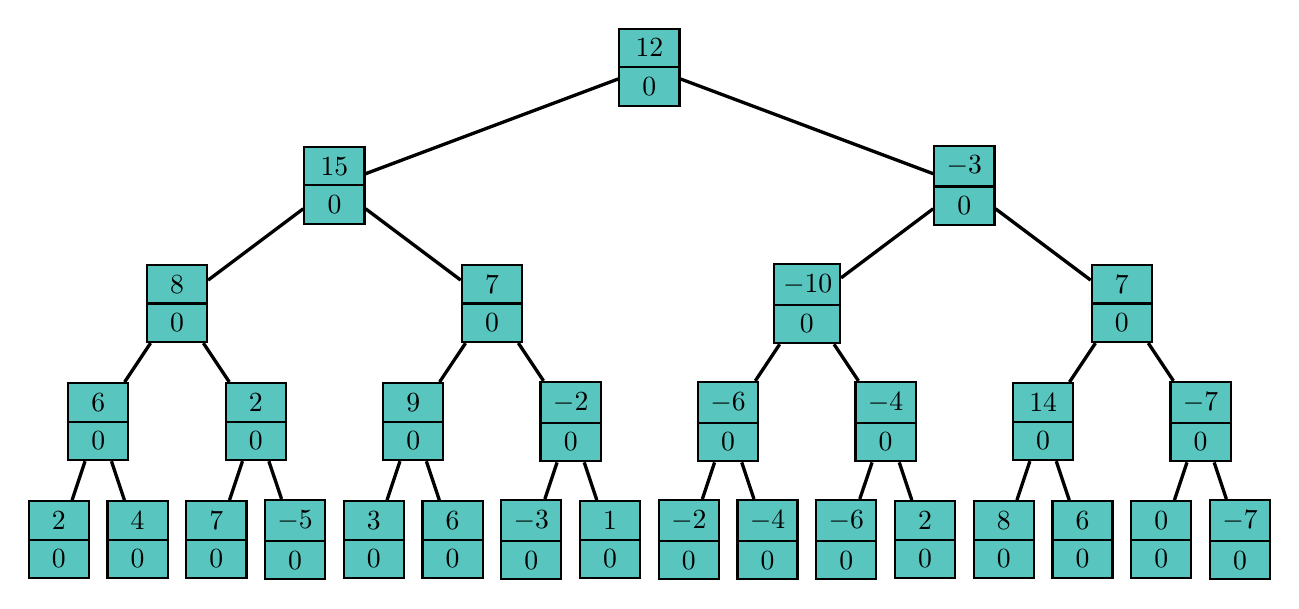
\begin{tikzpicture}[
  very thick,
  level 1/.style={sibling distance=80mm},
  level 2/.style={sibling distance=40mm},
  level 3/.style={sibling distance=20mm},
  level 4/.style={sibling distance=10mm},
  myrect/.style={
    draw,
    thick,
    fill=myseagreen,
    rectangle split,
    rectangle split parts=2,
    rectangle split part align=left,
    text width=3.5ex,
    text centered
    }
]
\node [myrect] (r){$12$\nodepart{two}0}
  child {
    node [myrect] (a) {15\nodepart{two}0}
    child {
      node [myrect] {8\nodepart{two}0}
      child {
        node [myrect] {6\nodepart{two}0}
        child {node [myrect] {2\nodepart{two}0}}
        child {node [myrect] {4\nodepart{two}0}}
      } 
      child {
        node [myrect] {2\nodepart{two}0}
        child {node [myrect] {7\nodepart{two}0}}
        child {node [myrect] {$-5$\nodepart{two}0}}
      }
    }
    child {
      node [myrect] {7\nodepart{two}0}
      child {node [myrect] {9\nodepart{two}0}
              child {node [myrect] {3\nodepart{two}0}}
        child {node [myrect] {6\nodepart{two}0}}
      }
      child {node [myrect] {$-2$\nodepart{two}0}
              child {node [myrect] {$-3$\nodepart{two}0}}
        child {node [myrect] {1\nodepart{two}0}}
      }
    }
  }
  child {
    node [myrect] {$-3$\nodepart{two}0}
    child {
      node [myrect, text width=4ex] {$-10$\nodepart{two}0}
      child {node [myrect] {$-6$\nodepart{two}0}
              child {node [myrect] {$-2$\nodepart{two}0}}
        child {node [myrect] {$-4$\nodepart{two}0}}}
      child {node [myrect] {$-4$\nodepart{two}0}
              child {node [myrect] {$-6$\nodepart{two}0}}
        child {node [myrect] {$2$\nodepart{two}0}}}
    }
    child {
      node [myrect] {7\nodepart{two}0}
      child {node [myrect] {14\nodepart{two}0}
              child {node [myrect] {8\nodepart{two}0}}
        child {node [myrect] {6\nodepart{two}0}}}
      child {node [myrect] {$-7$\nodepart{two}0}
              child {node [myrect] {0\nodepart{two}0}}
        child {node [myrect] {$-7$\nodepart{two}0}}}
    }
  };

\end{tikzpicture}
}
\end{center}

Once again, if the entire range associated with a node is contained within the update interval, we'll just make a note of it on that particular node and not update any of its children. We'll call such a node ``lazy.''

Here's the status of the tree after $update(3,12,2)$.

\begin{center}
{
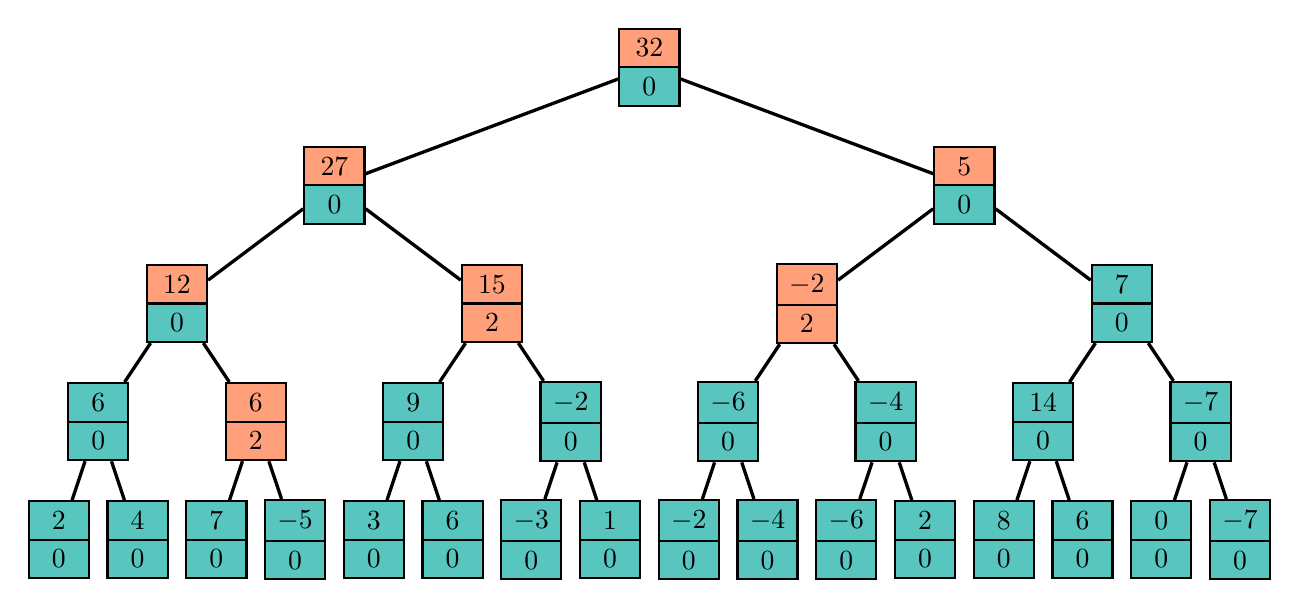
\begin{tikzpicture}[
  very thick,
  level 1/.style={sibling distance=80mm},
  level 2/.style={sibling distance=40mm},
  level 3/.style={sibling distance=20mm},
  level 4/.style={sibling distance=10mm},
  myrect/.style={
    draw,
    thick,
    rectangle split,
    rectangle split parts=2,
    rectangle split part fill={myseagreen, myseagreen},
    rectangle split part align=left,
    text width=3.5ex,
    text centered
    }
]
\node [myrect, rectangle split part fill={mysalmon, myseagreen}] (r){$32$\nodepart{two}0}
  child {
    node [myrect, rectangle split part fill={mysalmon, myseagreen}] (a) {27\nodepart{two}0}
    child {
      node [myrect, rectangle split part fill={mysalmon, myseagreen}] {12\nodepart{two}0}
      child {
        node [myrect] {6\nodepart{two}0}
        child {node [myrect] {2\nodepart{two}0}}
        child {node [myrect] {4\nodepart{two}0}}
      } 
      child {
        node [myrect, rectangle split part fill={mysalmon, mysalmon}] {6\nodepart{two}2}
        child {node [myrect] {7\nodepart{two}0}}
        child {node [myrect] {$-5$\nodepart{two}0}}
      }
    }
    child {
      node [myrect, rectangle split part fill={mysalmon, mysalmon}] {15\nodepart{two}2}
      child {node [myrect] {9\nodepart{two}0}
              child {node [myrect] {3\nodepart{two}0}}
        child {node [myrect] {6\nodepart{two}0}}
      }
      child {node [myrect] {$-2$\nodepart{two}0}
              child {node [myrect] {$-3$\nodepart{two}0}}
        child {node [myrect] {1\nodepart{two}0}}
      }
    }
  }
  child {
    node [myrect, rectangle split part fill={mysalmon, myseagreen}] {$5$\nodepart{two}0}
    child {
      node [myrect, rectangle split part fill={mysalmon, mysalmon}] {$-2$\nodepart{two}2}
      child {node [myrect] {$-6$\nodepart{two}0}
              child {node [myrect] {$-2$\nodepart{two}0}}
        child {node [myrect] {$-4$\nodepart{two}0}}}
      child {node [myrect] {$-4$\nodepart{two}0}
              child {node [myrect] {$-6$\nodepart{two}0}}
        child {node [myrect] {$2$\nodepart{two}0}}}
    }
    child {
      node [myrect] {7\nodepart{two}0}
      child {node [myrect] {14\nodepart{two}0}
              child {node [myrect] {8\nodepart{two}0}}
        child {node [myrect] {6\nodepart{two}0}}}
      child {node [myrect] {$-7$\nodepart{two}0}
              child {node [myrect] {0\nodepart{two}0}}
        child {node [myrect] {$-7$\nodepart{two}0}}}
    }
  };

\end{tikzpicture}
}
\end{center}

When a node is lazy, it indicates that the sum numbers of every other node in its subtree is no longer accurate. In particular, if a node is lazy, the sum number it keeps track of is not equal to the sum of the sum numbers of its children. This means whenever we need to access any node in that subtree, we'll need to update them then. Numbers in the tree therefore can change even after a query. Let's perform a query to illustrate that point.

$query(7,13)$ requires access to the nodes for the ranges $[7,8]$, $[9,12]$, and $[13,13]$. The nodes for $[9,12]$ and $[13,13]$ are up to date and store the correct sum, but the node for $[7,8]$ does not, as it is a descendent of the node for $[5,8]$, which has a nonzero lazy number. Highlighted are the nodes we'll need to update as we perform the query. Notice how $[5,8]$ simply passes its lazy number onto its children, and they update themselves as necessary.

\begin{center}
{
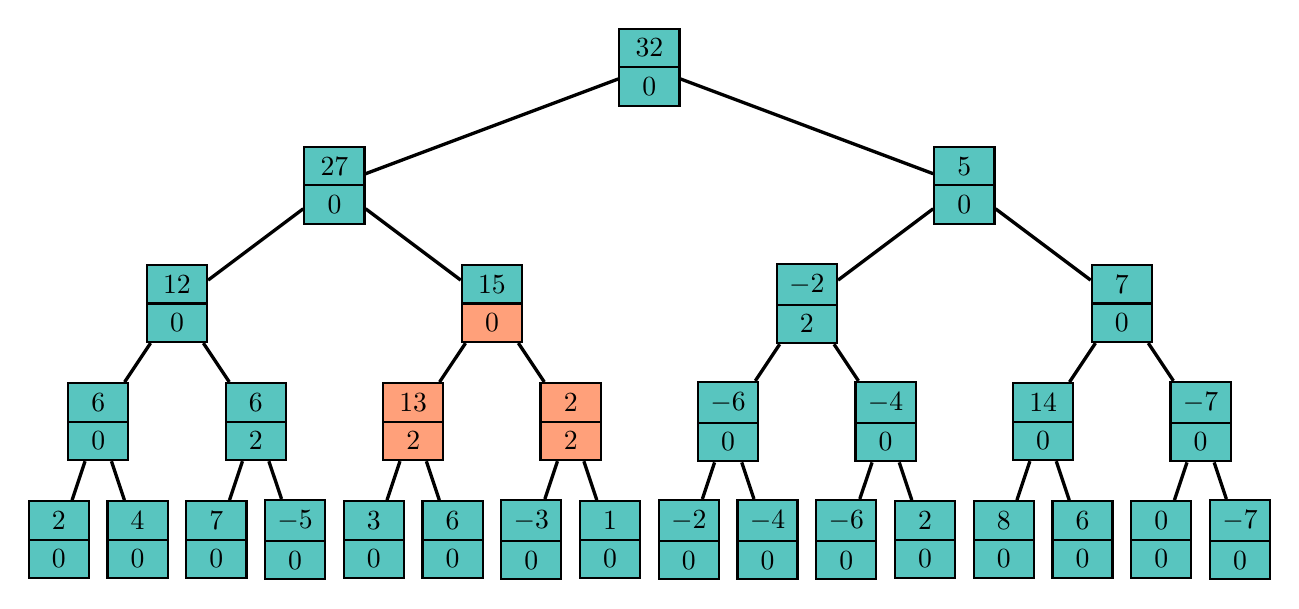
\begin{tikzpicture}[
  very thick,
  level 1/.style={sibling distance=80mm},
  level 2/.style={sibling distance=40mm},
  level 3/.style={sibling distance=20mm},
  level 4/.style={sibling distance=10mm},
  myrect/.style={
    draw,
    thick,
    rectangle split,
    rectangle split parts=2,
    rectangle split part fill={myseagreen, myseagreen},
    rectangle split part align=left,
    text width=3.5ex,
    text centered
    }
]
\node [myrect] (r){$32$\nodepart{two}0}
  child {
    node [myrect] (a) {27\nodepart{two}0}
    child {
      node [myrect] {12\nodepart{two}0}
      child {
        node [myrect] {6\nodepart{two}0}
        child {node [myrect] {2\nodepart{two}0}}
        child {node [myrect] {4\nodepart{two}0}}
      } 
      child {
        node [myrect] {6\nodepart{two}2}
        child {node [myrect] {7\nodepart{two}0}}
        child {node [myrect] {$-5$\nodepart{two}0}}
      }
    }
    child {
      node [myrect, rectangle split part fill={myseagreen, mysalmon}] {15\nodepart{two}0}
      child {node [myrect, rectangle split part fill={mysalmon, mysalmon}] {13\nodepart{two}2}
              child {node [myrect] {3\nodepart{two}0}}
        child {node [myrect] {6\nodepart{two}0}}
      }
      child {node [myrect, rectangle split part fill={mysalmon, mysalmon}] {$2$\nodepart{two}2}
              child {node [myrect] {$-3$\nodepart{two}0}}
        child {node [myrect] {1\nodepart{two}0}}
      }
    }
  }
  child {
    node [myrect] {$5$\nodepart{two}0}
    child {
      node [myrect] {$-2$\nodepart{two}2}
      child {node [myrect] {$-6$\nodepart{two}0}
              child {node [myrect] {$-2$\nodepart{two}0}}
        child {node [myrect] {$-4$\nodepart{two}0}}}
      child {node [myrect] {$-4$\nodepart{two}0}
              child {node [myrect] {$-6$\nodepart{two}0}}
        child {node [myrect] {$2$\nodepart{two}0}}}
    }
    child {
      node [myrect] {7\nodepart{two}0}
      child {node [myrect] {14\nodepart{two}0}
              child {node [myrect] {8\nodepart{two}0}}
        child {node [myrect] {6\nodepart{two}0}}}
      child {node [myrect] {$-7$\nodepart{two}0}
              child {node [myrect] {0\nodepart{two}0}}
        child {node [myrect] {$-7$\nodepart{two}0}}}
    }
  };

\end{tikzpicture}
}
\end{center}

Now, the nodes that we need are all up to date, and we can perform our query. This process is necessary whenever we are performing an operation on an interval that intersects but does not contain the range associated with a lazy node. Since this can only happen for two such nodes (one at either end of the interval in question), both updating and querying change values of at most four nodes per level, so both operations are $O(\log{n})$.

\section{Queue with Minimum Query}

Suppose we wanted a list data structure with the following three operations:

\begin{itemize}

\item
$add(x)$ -- add $x$ to the end of the list.

\item
$remove()$ -- remove the first element in the list.

\item
$min()$ -- return the minimum element in the list.

\end{itemize}

This is different from a heap since $remove$ does not remove the minimum element. It's pretty easy to find a $O(\log{n})$ solution using the data structures we already know. However, it is possible to build a data structure that can do any of these operations with complexity $O(1)$.

To solve this problem, we'll first solve an easier problem. Suppose instead of removing the first element of the list, we had remove the last element; in other words, we needed to build a stack with minimum query instead of a queue. This is a simple task; we'll just use a normal stack, but instead of storing single numbers, we'll store pairs. The pairs will each contain the number we're adding and the minimum element up to that point in the stack.

To build a queue given a stack with minimum query, we'll just have two stacks. When we add an element, we push it to the top of the first stack. When we remove an element, we take it off the top of the second stack. The minimum element in the queue is the smaller element between the minima of either stack.

This seems like it obviously doesn't work -- one of the stacks keeps growing, while the other can only shrink. This is not a problem, however; when the second stack runs out of elements, we'll just pop off every element of the first stack and push each onto the second stack. This amounts to one $O(n)$ operation for every $n$ $O(1)$ operations, which averages out to constant time.

\section{Balanced Binary Search Tree}

Recall that a normal binary search tree is not guaranteed to be balanced. Many data structures have been invented to self-balance the binary search tree.

The \textit{red-black tree} was an early development that represents the ``just do it'' approach, using casework to balance a tree. This results in a simple mathematical proof for the maximum depth of the tree. Unfortunately, coding these up are quite nasty do to the casework involved, so doing so is generally not preferred unless your name is Sreenath Are.

The \textit{splay tree} is a data structure that guarantees amortized logarithmic performance; this means that any single operation is not necessarily linear, but over \textit{any} sequence of length $m$ for $m \ge n$, the performance for all $m$ operations is $O(m \log{n})$. Though the proof of the splay tree's complexity is necessarily more complicated than the red-black tree's complexity, as it requires amortized analysis, coding the splay tree is much easier than coding the red-black tree. In addition, the splay tree grants us more flexibility than the red-black tree provides, allowing us to build more complicated structures like link-cut trees using splay trees.

The \textit{treap} is a probabilistic data structure that combines the BST with a heap to usually create a balanced tree. Just as quicksort is not guaranteed to run in $O(n\log{n})$, so too does the treap not guarantee $O(\log{n})$ operations, but will usually result in logarithmic performance.

\subsection{Tree Rotation}

The key idea behind all of these data structures is the use of the \textit{tree rotation}, which is used to change the structure of the tree but will not change the order of the elements (inorder). Maintaining the order of the elements is important, of course, if we wish our tree to remain a binary search tree.

\begin{center}
\begin{tikzpicture}[very thick,level/.style={sibling distance=35mm/#1}, auto, bend left]

\node [vertex, fill=mysalmon] (r){$Q$}
  child {
  	node[vertex, fill=mysalmon] {$P$}
  	child {
  		node[vertex] {$A$} {
		node[draw, isosceles triangle, shape border uses incircle, fill=myseagreen, minimum height = 1.275cm, shape border rotate=90, yshift=-1.40cm] {} }
  	}
  	child {
  		node[vertex] {$B$} {
		node[draw, isosceles triangle, shape border uses incircle, fill=myseagreen, minimum height = 1.275cm, shape border rotate=90, yshift=-1.40cm] {} }
  	}
  }
  child {
  		node[vertex] (r3) {$C$} {
		node[draw, isosceles triangle, shape border uses incircle, fill=myseagreen, minimum height = 1.275cm, shape border rotate=90, yshift=-1.40cm] {} }
};

\node[vertex, fill=mysalmon] [right=8cm of r] (r2) {$P$}
  child {
  		node[vertex] (r4) {$A$} {
		node[draw, isosceles triangle, shape border uses incircle, fill=myseagreen, minimum height = 1.275cm, shape border rotate=90, yshift=-1.40cm] {} }
  }
  child {
  	node[vertex, fill=mysalmon] {$Q$}
	child {
  		node[vertex] {$B$} {
		node[draw, isosceles triangle, shape border uses incircle, fill=myseagreen, minimum height = 1.275cm, shape border rotate=90, yshift=-1.40cm] {} }
  	}
	child {
  		node[vertex] {$C$} {
		node[draw, isosceles triangle, shape border uses incircle, fill=myseagreen, minimum height = 1.275cm, shape border rotate=90, yshift=-1.40cm] {} }
	}
};

\coordinate[right=of r3] (a);
\coordinate[left=of r4] (b);

\coordinate[below=of a] (c);
\coordinate[below=of b] (d);

\draw[->] (a) to node {rotate right} (b);
\draw[->] (d) to node {rotate left} (c);

\end{tikzpicture}
\end{center}

Here, the triangles represent subtrees, as $A$, $B$, and $C$ could very well have children of our own, but they are not shown in the diagram. Note that the inorder ordering of the nodes has not been changed.

When we rotate right, we literally take the edge connecting $P$ and $Q$ and rotate it clockwise. Then $P$ becomes the parent of $Q$ where before $P$ was the child of $Q$. However, this definition of rotation is somewhat cumbersome, as we have different terms for the highly symmetrical rotating right and rotating left. The key characteristic a rotation is we move the lower node up one level. Thus, I prefer to think of tree rotation as whatever tree rotation, either left or right, will \textit{rotate up} a node. In the diagram, rotating right is analogous to rotating $P$ up, and rotating left is analogous to rotating $Q$ up. Rotating a node up will change the tree such that its former parent is now its child.

The other notable change in the tree structure is the subtree associated with $B$ passes between $P$ and $Q$ upon tree rotation. Finally, tree rotation can happen at any place in the tree, not just at the root. When we rotate $P$ up, we must update the parent of $Q$ to change its child to $P$.

\begin{center}
\begin{tikzpicture}[very thick,level 2/.style={sibling distance=35mm}, level 3/.style={sibling distance=35mm/2}, level 4/.style={sibling distance=35mm/3}, level 1/.style={sibling distance=50mm}, auto, bend left]

\node [vertex] (r) {$D$}
	child{node[vertex, fill=mysalmon] {$Q$}
  child {
  	node[vertex, fill=mysalmon] {$P$}
  	child {
  		node[vertex] {$A$} 
  		child [missing]
  		child{
  			node [vertex] {$E$}
  		}
  	}
  	child {
  		node[vertex] {$B$}
  } }
  child {
  		node[vertex] (r3) {$C$}
}} 
  		child [missing];

\node[vertex] [right=8cm of r] (r2) {$D$}
	child{node[vertex, fill=mysalmon] {$P$}
  child {
  		node[vertex] (r4) {$A$} 
  		child [missing]
  		child{
  			node [vertex] {$E$}
  		}
  }
  child {
  	node[vertex, fill=mysalmon] {$Q$}
	child {
  		node[vertex] {$B$} 
  	}
	child {
  		node[vertex] {$C$} 
	}
}}
child[missing];

\coordinate[right=of r3] (a);
\coordinate[left=of r4] (b);

\coordinate[below=of a] (c);
\coordinate[below=of b] (d);

\draw[->] (a) to node {rotate $P$} (b);
\draw[->] (d) to node {rotate $Q$} (c);

\end{tikzpicture}
\end{center}

Note that in this example, rotating up $P$ decreases the total height of the tree. We want to somehow systematically rotate up nodes to accomplish this. The following data structures provide such a system.

\subsection{Red-Black Tree}

As stated earlier, the red-black tree represents the ``just do it'' approach. We want to somehow bound the maximum length from the root to any leaf node by applying a constraint on the tree. In this case, our constraint is a coloring of the nodes (red or black) such certain properties are satisfied. For the red-black tree, the only nodes storing data are non-leaf nodes, and all leaf nodes store ``null.'' The number of null nodes, then, is $n+1$, where $n$ is the number of non-null nodes. We do this so that any node storing useful information has two children.

We want our tree to satisfy the following properties:

\begin{enumerate}

\item
The root is black.

\item
All leaf nodes (null) are black.

\item
Every red node has two black children. Consequently, a red node has a black parent.

\item
Any path from the root to a null node contains the same number of black elements.

\end{enumerate}

\begin{center}
\begin{tikzpicture}[very thick,
%level 1/.style={sibling distance=80mm},
%level 2/.style={sibling distance=50mm},
%level 3/.style={sibling distance=30mm},
%level 4/.style={sibling distance=20mm},
%level 5/.style={sibling distance=10mm},
%level 6/.style={sibling distance=10mm},
rv/.style={
	draw,circle,minimum size=24pt,inner sep=0pt, fill=myred
},
bv/.style={
	draw,circle,minimum size=24pt,inner sep=0pt, text=mywhite, fill=myblack
},
br/.style={
	draw,
    thick,
    fill=myblack,
    text width=4ex,
    text centered,
    text=mywhite
}
]

\node[bv] {$M$} [sibling distance=80mm]
	child {
		node[bv] {$D$} [sibling distance=50mm]
			child {
				node[bv] {$A$} [sibling distance=15mm]
					child {
						node[br] {null}
					}
					child {
						node[rv] {$C$} [sibling distance=10mm]
							child {
								node[br] {null}
							}
							child {
								node[br] {null}
							}
					}
			}
			child {
				node[rv]{$K$} [sibling distance=30mm]
					child {
						node[bv]{$G$} [sibling distance=20mm]
							child {
								node[rv]{$E$} [sibling distance=10mm]
									child{
										node[br]{null}
									}
									child{
										node[br]{null}
									}
							}
							child {
								node[rv]{$I$} [sibling distance=10mm]
									child {
										node[br]{null}
									}
									child {
										node[br]{null}
									}
							}
					}
					child {
						node[bv]{$L$} [sibling distance=10mm]
							child {
								node[br]{null}
							}
							child {
								node[br]{null}
							}
					}
			}
	}
	child {
		node[bv]{$T$} [sibling distance=40mm]
			child {
				node[bv] {$Q$} [sibling distance=15mm]
					child {
						node[br] {null}
					}
					child {
						node[rv]{$R$} [sibling distance=10mm]
							child{
								node[br]{null}
							}
							child{
								node[br]{null}
							}
					}
			}
			child {
				node[rv] {$X$} [sibling distance=20mm]
					child {
						node[bv] {$V$} [sibling distance=10mm]
							child{
								node[br]{null}
							}
							child{
								node[br]{null}
							}
					}
					child {
						node[bv] {$Z$} [sibling distance=10mm]
							child{
								node[br]{null}
							}
							child{
								node[br]{null}
							}
					}
			}
	}
;

\end{tikzpicture}
\end{center}

Note that every path from the root to a null node contains four black nodes.

The proof of $O(\log{n})$ search follows immediately. The shortest possible path contains only black nodes, and the longest possible path contains black and red nodes alternating. Since the number of black nodes in both must be the same, any path is at most twice as long as any other path. As the number of nodes in the tree is $2n+1$, the number of black nodes $m$ in any path is then bounded below by $2^{2m} - 1 \ge 2n + 1$ and above by $2^{m} - 1 \le 2n + 1$. Thus the height of the tree is on the order $O(\log{n})$, and we are done.

Thus if our tree maintains its red-black coloring and satisfies the necessary properties, we can guarantee that our tree is balanced. We then consider the two ways we change the state of the tree, insertion and deletion. We can insert and delete in the normal way, but we might need to make changes to the tree after that to restore the red-black properties. We do this through a small number of color flips and tree rotations, which we can handle through casework.

Let's handle insertion first. When we insert a node, it takes the place of a black null leaf node. To maintain property 4, we must color the new node red, as it has two black null children. However, we may have violated some of the other properties, specifically 1 and 3.

We'll call the new node $N$, its parent $P$, its uncle (parent's sibling) $U$, and its grandparent $G$, if they exist.

We consider the following five cases.

\begin{enumerate}

\item
$N$ is the root node. That is, $N$ is the first node added to the tree.

It is easy to just change the color of $N$ to red to restore property 1, and we are done.

\item
$P$ is black.

Then property 3 is not violated, and we are done.

\item
$P$ is red, and $U$ is red ($G$ and $U$ exist since $P$ cannot be the root, as the root is black).

As $P$ and $U$ are red, $G$ is black. We simply color $P$ and $U$ black and $G$ red to restore property 3.

\begin{center}
\begin{tikzpicture}[very thick,
rv/.style={
	draw,circle,minimum size=24pt,inner sep=0pt, fill=myred
},
bv/.style={
	draw,circle,minimum size=24pt,inner sep=0pt, text=mywhite, fill=myblack
},
br/.style={
	draw,
    thick,
    fill=myblack,
    text width=4ex,
    text centered,
    text=mywhite
},
level/.style={sibling distance=35mm/#1}, auto]

\node[bv] (r) {$G$}
child {
	node[rv] {$P$}
	child {
		node[rv] {$N$}
	}
	child [missing]
}
child {
	node[rv] (r3) {$U$} 
};

\node[rv] [right=8cm of r] (r2) {$G$}
child {
	node[bv] (r4) {$P$}
	child {
		node[rv] {$N$}
	}
	child[missing]
}
child {
	node[bv] {$U$}
};

\coordinate[right=of r3] (a);
\coordinate[left=of r4] (b);

\draw[->] (a) to (b);

\end{tikzpicture}
\end{center}

\item
$P$ is red, $U$ is black, and $N$ is on the same side of $P$ as $P$ is of $G$.

$G$ must be black. We rotate up $P$ and color $P$ black and $G$ red.

\begin{center}
\begin{tikzpicture}[very thick,
rv/.style={
	draw,circle,minimum size=24pt,inner sep=0pt, fill=myred
},
bv/.style={
	draw,circle,minimum size=24pt,inner sep=0pt, text=mywhite, fill=myblack
},
br/.style={
	draw,
    thick,
    fill=myblack,
    text width=4ex,
    text centered,
    text=mywhite
},
level/.style={sibling distance=35mm/#1}, auto]

\node[bv] (r) {$G$}
child {
	node[rv] {$P$}
	child {
		node[rv] {$N$}
	}
	child [missing]
}
child {
	node[bv] (r3) {$U$} 
};

\node[bv] [right=8cm of r] (r2) {$P$}
child {
	node[rv] (r4) {$N$} 
}
child {
	node[rv] {$G$}
	child[missing]
	child {
		node[bv] {$U$}
	}
};

\coordinate[right=of r3] (a);
\coordinate[left=of r4] (b);

\draw[->] (a) to (b);

\end{tikzpicture}
\end{center}

\item
$P$ is red, $U$ is black, and $N$ is on the opposite side of $P$ as $P$ is of $G$.

$G$ must be black. We rotate up $N$, and this reduces to case 4.

\begin{center}
\begin{tikzpicture}[very thick,
rv/.style={
	draw,circle,minimum size=24pt,inner sep=0pt, fill=myred
},
bv/.style={
	draw,circle,minimum size=24pt,inner sep=0pt, text=mywhite, fill=myblack
},
br/.style={
	draw,
    thick,
    fill=myblack,
    text width=4ex,
    text centered,
    text=mywhite
},
level/.style={sibling distance=35mm/#1}, auto]

\node[bv] (r) {$G$}
child {
	node[rv] {$P$} 
	child[missing]
	child {
		node[rv] {$N$} 
	}
}
child {
	node[bv] (r3) {$U$}
};

\node[bv] [right=8cm of r] (r2) {$G$}
child {
	node[rv] (r4) {$N$}
	child {
		node[rv] {$P$}
	}
	child[missing]
}
child {
	node[bv] {$U$} 
};

\coordinate[right=of r3] (a);
\coordinate[left=of r4] (b);

\draw[->] (a) to (b);

\end{tikzpicture}
\end{center}

\end{enumerate}

Thus after we insert, we can always restructure the tree using a constant number of operations to restore the necessary red-black tree properties.

Now we need to work on deletion. Recall how deletion works on a normal binary search tree. If the node we need to replace has two children, we swap the node with the least element in its right subtree, which does not have two children. We then are able to remove that node more easily.

We can do the same thing with the red-black tree. If a node has two non-null children, we swap its value with the least non-null node in its right subtree and remove that node. Thus we reduce the deletion problem to the case where the node we need to remove has at least one null child.

Two cases are very easy.

\begin{enumerate}

\item
The node we wish to remove is red.

Then the node must have two null leaf nodes as children. Then we remove the node by replacing it and its children with a single null node.

\item
The node is black and has a red child.

We replace the node with its child and paint its child red.

\end{enumerate}

The remaining case is the node black with two black null children. We'll first replace the node with a null node $N$. Then, all paths passing through $N$ are one black node short compared to all other paths.

We denote the parent of $N$ as $P$, its sibling $S$, and its sibling's children $C$ and $F$, such that $C$ is on the same side of $S$ as $N$ is of $P$, if they exist. That is, $C$ is the ``closer nephew'' child, while $F$ is the farther. We now describe a six-case balancing procedure on the black node $N$ that fixes our problem.

\begin{enumerate}

\item
$N$ is the root.

We are done, as every path possible must pass through $N$, so all paths are balanced.

\item
$P$ is red and $S$, $C$, and $F$ are black.

Then we simply trade the colors of $P$ and $S$. The number of black nodes for paths passing through $S$ stays the same, but the number of black nodes for paths passing through $N$ increases, so we are done.

\begin{center}
\begin{tikzpicture}[very thick,
rv/.style={
	draw,circle,minimum size=24pt,inner sep=0pt, fill=myred
},
bv/.style={
	draw,circle,minimum size=24pt,inner sep=0pt, text=mywhite, fill=myblack
},
br/.style={
	draw,
    thick,
    fill=myblack,
    text width=4ex,
    text centered,
    text=mywhite
},
level/.style={sibling distance=35mm/#1}, auto]

\node[rv] (r) {$P$}
child {
	node[bv] {$N$} 
}
child {
	node[bv] (r3) {$S$}
	child {
		node[bv] {$C$}
	}
	child {
		node[bv] {$F$}
	}
};

\node[bv] [right=8cm of r] (r2) {$P$}
child {
	node[bv] (r4) {$N$} 
}
child {
	node[rv] {$S$}
	child {
		node[bv] {$C$}
	}
	child {
		node[bv] {$F$}
	}
};

\coordinate[right=of r3] (a);
\coordinate[left=of r4] (b);

\draw[->] (a) to (b);

\end{tikzpicture}
\end{center}

\item
$S$ is black and $F$ is red.

Then we color $F$ black and rotate up $S$, before swapping the colors of $P$ and $S$. Then paths passing through $N$ gain a black vertex, while paths passing through $C$ and $F$ stay the same.

\begin{center}
\begin{tikzpicture}[very thick,
rv/.style={
	draw,circle,minimum size=24pt,inner sep=0pt, fill=myred
},
bv/.style={
	draw,circle,minimum size=24pt,inner sep=0pt, text=mywhite, fill=myblack
},
br/.style={
	draw,
    thick,
    fill=myblack,
    text width=4ex,
    text centered,
    text=mywhite
},
level/.style={sibling distance=35mm/#1}, auto]

\node[vertex] (r) {$P$}
child {
	node[bv] {$N$} 
}
child {
	node[bv] (r3) {$S$}
	child {
		node[vertex] {$C$}
	}
	child {
		node[rv] {$F$}
	}
};

\node[vertex] [right=8cm of r] (r2) {$S$}
child {
	node[bv] (r4) {$P$} 
	child {
		node[bv] {$N$}
	}
	child {
		node[vertex] {$C$}
	}
}
child {
	node[bv] {$F$}
};

\coordinate[right=of r3] (a);
\coordinate[left=of r4] (b);

\draw[->] (a) to (b);

\end{tikzpicture}
\end{center}

\item
$S$ is black, $F$ is black, and $C$ is red.

Then we rotate up $C$ and swap the colors of $S$ and $C$. Then this reduces to case 3.

\begin{center}
\begin{tikzpicture}[very thick,
rv/.style={
	draw,circle,minimum size=24pt,inner sep=0pt, fill=myred
},
bv/.style={
	draw,circle,minimum size=24pt,inner sep=0pt, text=mywhite, fill=myblack
},
br/.style={
	draw,
    thick,
    fill=myblack,
    text width=4ex,
    text centered,
    text=mywhite
},
level/.style={sibling distance=35mm/#1}, auto]

\node[vertex] (r) {$P$}
child {
	node[bv] {$N$} 
}
child {
	node[bv] (r3) {$S$}
	child {
		node[rv] {$C$}
	}
	child {
		node[bv] {$F$}
	}
};

\node[vertex] [right=8cm of r] (r2) {$P$}
child {
	node[bv] (r4) {$N$} 
}
child {
	node[bv] {$C$}
		child [missing]
		child {
			node[rv] {$S$}
				child [missing]
				child {
					node[bv] {$F$}
				}
		}
};

\coordinate[right=of r3] (a);
\coordinate[left=of r4] (b);

\draw[->] (a) to (b);

\end{tikzpicture}
\end{center}

\item
$S$ is red.

Then $P$, $C$, and $F$ must be black. We rotate $S$ up and swap the colors of $P$ and $S$. $C$, the new sibling of $N$ is black, so this then reduces to one of cases 2, 3, or 4.

\begin{center}
\begin{tikzpicture}[very thick,
rv/.style={
	draw,circle,minimum size=24pt,inner sep=0pt, fill=myred
},
bv/.style={
	draw,circle,minimum size=24pt,inner sep=0pt, text=mywhite, fill=myblack
},
br/.style={
	draw,
    thick,
    fill=myblack,
    text width=4ex,
    text centered,
    text=mywhite
},
level/.style={sibling distance=35mm/#1}, auto]

\node[bv] (r) {$P$}
child {
	node[bv] {$N$} 
}
child {
	node[rv] (r3) {$S$}
	child {
		node[bv] {$C$}
	}
	child {
		node[bv] {$F$}
	}
};

\node[bv] [right=8cm of r] (r2) {$S$}
child {
	node[rv] (r4) {$P$} 
		child {
			node[bv] {$N$}
		}
		child {
			node[bv] {$C$}
		}
}
child {
	node[bv] {$F$}
};

\coordinate[right=of r3] (a);
\coordinate[left=of r4] (b);

\draw[->] (a) to (b);

\end{tikzpicture}
\end{center}

\item
$P$, $S$, $C$, and $F$ are all black.

Then we recolor $S$ red. Now, all paths through $P$ have the same number of black nodes, but each path through $P$ has one less black node than each path not passing through $P$. Since $P$ is black, and this procedure did not require that $N$ be a leaf node, we can repeat this entire balancing procedure on $P$.

\begin{center}
\begin{tikzpicture}[very thick,
rv/.style={
	draw,circle,minimum size=24pt,inner sep=0pt, fill=myred
},
bv/.style={
	draw,circle,minimum size=24pt,inner sep=0pt, text=mywhite, fill=myblack
},
br/.style={
	draw,
    thick,
    fill=myblack,
    text width=4ex,
    text centered,
    text=mywhite
},
level/.style={sibling distance=35mm/#1}, auto]

\node[bv] (r) {$P$}
child {
	node[bv] {$N$} 
}
child {
	node[bv] (r3) {$S$}
	child {
		node[bv] {$C$}
	}
	child {
		node[bv] {$F$}
	}
};

\node[bv] [right=8cm of r] (r2) {$P$}
child {
	node[bv] (r4) {$N$} 
}
child {
	node[rv] {$S$}
	child {
		node[bv] {$C$}
	}
	child {
		node[bv] {$F$}
	}
};
\coordinate[right=of r3] (a);
\coordinate[left=of r4] (b);

\draw[->] (a) to (b);

\end{tikzpicture}
\end{center}

\end{enumerate}

Unlike the balancing for insertions, the balancing for deletions has the potential to call itself on the parent node $P$. However, balancing following a deletion is still $O(\log{n})$ worst case. It is possible prove that it is $O(1)$ amortized. Regardless, we now have a deletion algorithm that runs in $O(\log{n})$ time.

Thus the red-black tree supports standard binary search tree operations, all in $O(\log{n})$.

\subsection{Splay Tree}

Remember that rotating a node brings it one level closer to the root. The idea behind a splay tree is to apply a sequence of rotations that rotate a node all the way up to the root. The intuition for doing this is once we access a node, it is easy to perform other operations on it since it will simply be the root of the tree.

It is not at all clear that rotating nodes to the root will somehow improve the average performance of the tree. That's because rotating the normal way doesn't! To improve the performance of the tree, we expect that our balancing procedure tends to decrease the height of the tree. Unfortunately, simply repeatedly rotating a node up the tree doesn't exactly do that task. Consider a tree that looks liked a linked list, and rotating the nodes in the order $A$, $B$, $C$, $D$, as shown in the diagram. The height of the tree remains linear in magnitude, as at its smallest stage the tree is around $\frac{n}{2}$ in height, so accessing elements remains $O(n)$ on average.

\begin{center}
\begin{tikzpicture}[very thick,sibling distance=15mm, auto]

\node [vertex] (r) {$D$}
child {
	node [vertex] (r3) {$C$}
		child {
			node [vertex] {$B$}
				child {
					node[vertex] {$A$}
				}
				child[missing]
		}
		child[missing]
}
child[missing];

\node[vertex] [right=0.8cm of r] (r2) {$A$}
child[missing]
child {
	node [vertex] (r4) {$D$}
		child {
			node [vertex] {$C$}
				child {
					node[vertex] {$B$}
				}
				child[missing]
		}
		child[missing]
};

\node[vertex] [right=2.8cm of r2] (r6) {$B$}
child {
	node [vertex] (r5) {$A$}
}
child {
	node [vertex] (r7) {$D$}
		child {
			node[vertex] {$C$}
		}
		child[missing]
};

\node [vertex] [right=2.8 of r6] (r8) {$C$}
child {
			node [vertex] (r9) {$B$}
				child {
					node[vertex] {$A$}
				}
				child[missing]
}
child{
	node [vertex] (r10) {$D$}
};

\node [vertex] [right=2.8cm of r8] (r11) {$D$}
child {
	node [vertex] (r12) {$C$}
		child {
			node [vertex] {$B$}
				child {
					node[vertex] {$A$}
				}
				child[missing]
		}
		child[missing]
}
child[missing];

\coordinate[right=0.25cm of r3] (a);
\coordinate[left=0.25cm of r4] (b);
\coordinate[right=0.25cm of r4] (c);
\coordinate[left=0.25cm of r5] (d);
\coordinate[right=0.25cm of r7] (e);
\coordinate[left=0.25cm of r9] (f);
\coordinate[right=0.25cm of r10] (g);
\coordinate[left=0.25cm of r12] (h);

\draw[->] (a) to node {rot. $A$} (b);

\draw[->] (c) to node {rot. $B$} (d);

\draw[->] (e) to node {rot. $C$} (f);

\draw[->] (g) to node {rot. $D$} (h);

\end{tikzpicture}
\end{center}

As discussed earlier, simply repeatedly applying the standard rotation clearly is not guaranteed to reduce the height of the tree on average. However, if we simply make one small change, magic happens. The trick of the splay tree is to rotate a node to the root in such a way that the tree has a tendency to decrease in height. We'll use two compound rotations, and depending on the structure of the tree, we'll use a different one accordingly, to rotate a node to the root.

When a node is a left child and its parent is a left child, or the node is a right child and its parent is a right child, we first rotate up the parent, and then rotate up the node. This sequence of rotations is the only difference between splaying and rotating a node to the root using standard rotation.

\begin{center}
\begin{tikzpicture}[very thick,sibling distance=25mm, auto]

\node [vertex] (r) {$Z$}
	child {
		node [vertex] {$Y$}
			child {
				node [vertex] {$X$}
				  	child {
  		node [vertex] {$A$} {
		node [draw, isosceles triangle, shape border uses incircle, fill=myseagreen, minimum height = 1.275cm, shape border rotate=90, yshift=-1.40cm] {} }
  	}
				  	child {
  		node [vertex] {$B$} {
		node [draw, isosceles triangle, shape border uses incircle, fill=myseagreen, minimum height = 1.275cm, shape border rotate=90, yshift=-1.40cm] {} }
  	}
			}
  	child {
  		node [vertex] {$C$} {
		node [draw, isosceles triangle, shape border uses incircle, fill=myseagreen, minimum height = 1.275cm, shape border rotate=90, yshift=-1.40cm] {} }
  	}
	}
  	child {
  		node [vertex] (r3) {$D$} {
		node [draw, isosceles triangle, shape border uses incircle, fill=myseagreen, minimum height = 1.275cm, shape border rotate=90, yshift=-1.40cm] {} }
  	};

\node[vertex] [right=6cm of r] (r2) {$X$}
  	child {
  		node [vertex] (r4) {$A$} {
		node [draw, isosceles triangle, shape border uses incircle, fill=myseagreen, minimum height = 1.275cm, shape border rotate=90, yshift=-1.40cm] {} }
  	}
child {
	node [vertex] {$Y$}
  	child {
  		node [vertex] {$B$} {
		node [draw, isosceles triangle, shape border uses incircle, fill=myseagreen, minimum height = 1.275cm, shape border rotate=90, yshift=-1.40cm] {} }
  	}
		child {
			node [vertex] {$Z$}
	  	child {
  		node [vertex] {$C$} {
		node [draw, isosceles triangle, shape border uses incircle, fill=myseagreen, minimum height = 1.275cm, shape border rotate=90, yshift=-1.40cm] {} }
  	}
	child {
  		node [vertex] {$D$} {
		node [draw, isosceles triangle, shape border uses incircle, fill=myseagreen, minimum height = 1.275cm, shape border rotate=90, yshift=-1.40cm] {} }
  	}
		}
};

\coordinate[right=of r3] (a);
\coordinate[left=of r4] (b);

\draw[->] (a) to node {rotate $Y$, rotate $X$} (b);

\end{tikzpicture}
\end{center}

When a node is a left child and its parent is a right child, or the node is a right child and its parent is a left child, we rotate the node up twice, the normal way.

\begin{center}
\begin{tikzpicture}[very thick, auto]

\node [vertex] (r) {$Z$} [sibling distance=25mm]
	child {
		node [vertex] {$Y$}
			child {
  		node [vertex] {$A$} {
		node [draw, isosceles triangle, shape border uses incircle, fill=myseagreen, minimum height = 1.275cm, shape border rotate=90, yshift=-1.40cm] {} }
  	}
			child {
				node [vertex] {$X$} [sibling distance=15mm]
				  	child {
  		node [vertex] {$B$} {
		node [draw, isosceles triangle, shape border uses incircle, fill=myseagreen, minimum height = 1.275cm, shape border rotate=90, yshift=-1.40cm] {} }
  	}
				  	child {
  		node [vertex] {$C$} {
		node [draw, isosceles triangle, shape border uses incircle, fill=myseagreen, minimum height = 1.275cm, shape border rotate=90, yshift=-1.40cm] {} }
  	}
			}
	}
  	child {
  		node [vertex] (r3) {$D$} {
		node [draw, isosceles triangle, shape border uses incircle, fill=myseagreen, minimum height = 1.275cm, shape border rotate=90, yshift=-1.40cm] {} }
  	};

\node[vertex] [right=7cm of r] (r2) {$X$} [sibling distance=30mm]
child {
	node [vertex] (r4) {$Y$} [sibling distance=15mm]
  	child {
  		node [vertex] {$A$} {
		node [draw, isosceles triangle, shape border uses incircle, fill=myseagreen, minimum height = 1.275cm, shape border rotate=90, yshift=-1.40cm] {} }
  	}
  	child {
  		node [vertex] {$B$} {
		node [draw, isosceles triangle, shape border uses incircle, fill=myseagreen, minimum height = 1.275cm, shape border rotate=90, yshift=-1.40cm] {} }
  	}
  	}
	child {
			node [vertex] {$Z$} [sibling distance=15mm]
	  	child {
  		node [vertex] {$C$} {
		node [draw, isosceles triangle, shape border uses incircle, fill=myseagreen, minimum height = 1.275cm, shape border rotate=90, yshift=-1.40cm] {} }
  	}
	child {
  		node [vertex] {$D$} {
		node [draw, isosceles triangle, shape border uses incircle, fill=myseagreen, minimum height = 1.275cm, shape border rotate=90, yshift=-1.40cm] {} }
  	}
};

\coordinate[right=of r3] (a);
\coordinate[left=of r4] (b);

\draw[->] (a) to node {rotate $X$, rotate $X$} (b);

\end{tikzpicture}
\end{center}

Finally, when a node's parent is the root, so it has no grandparent, we simply rotate up the normal way.

Rotating a node to the root in this way is called \textit{splaying} the node. Thus, splaying a node brings it to the root of the tree. Splaying seems too simple to lead to an amortized $O(\log{n})$ solution. To get a better idea of how splaying works, let's see what it does to a tree that looks like a linked list.

\begin{center}
\begin{tikzpicture}[very thick,sibling distance=15mm, auto]

\node [vertex] (r) {$G$}
		child {
		node [vertex] {$F$}
		child {
		node [vertex] (r3) {$E$}
		child {
		node [vertex] {$D$}
		child {
		node [vertex] {$C$}
		child {
		node [vertex] {$B$}
		child {
		node [vertex] {$A$}
		}
		child [missing]
		}
		child [missing]
		}
		child [missing]
		}
		child [missing]
		}
		child [missing]
		}
		child [missing]
;

\node[vertex] [right=6cm of r] (r2) {$A$}
child[missing]
child {
	node[vertex] {$F$}
	child {
		node[vertex] (r4) {$D$}
		child {
		node[vertex] {$B$}
		child [missing]
	child {
		node[vertex] {$C$}
	}
	}
	child {
		node[vertex] {$E$}
	}
	}
	child {
		node[vertex] {$G$}
	}
};

\coordinate[right=of r3] (a);
\coordinate[left=of r4] (b);

\draw[->] (a) to node {splay $A$} (b);

\end{tikzpicture}
\end{center}

Splaying here cuts the height of the tree in half -- a huge improvement. Splaying is not guaranteed to decrease the height of the tree, and it is possible for a sequence of splays to even result in a linked-list-like structure. However, given a number $m$ at least equal to the maximum number of nodes $n$ ever in the tree, \textit{any} sequence of $m$ splays runs in $O(m \log{n})$. Splaying is then $O(\log{n})$, amortized.\footnote{If you're curious to see the proof of this, a rather in depth explanation can be found here: \url{http://www.cs.cmu.edu/afs/cs/academic/class/15859-f05/www/documents/splay-trees.txt}}

Then, whenever we access a node, even in insertion and deletion, we splay that node to the top. This makes access, insert, and delete all $O(\log{n})$ amortized.

Since splay trees need not satisfy a restrictive coloring, as red-black trees do, we have the freedom to completely change the structure of the tree at a whim. Recall how tedious the casework was to simply add or remove one node at a time in a red-black tree. Because the splay tree is simply a normal binary search tree that rotates nodes up upon access, we can detach an entire subtree from the tree and not worry about any properties of our tree no longer being satisfied.

For this reason, we define the \textit{split} and \textit{join} functions for splay trees.

Given two trees $S$ and $T$, such that every element in $S$ is less than every element in $T$, we join $S$ and $T$ into one tree by splaying the largest element in $S$, so that the root, which is now the largest element, has no right child. Then, we set its right child to the root of $T$, resulting in a single tree with elements from both $S$ and $T$.

Given a tree and a value $v$, we split the tree in two by splaying the greatest element not greater than $v$ to the root and detaching the right subtree from the rest. This results in two trees, one containing all elements at most $v$, and the other containing all elements greater than $v$.

Both of these operations are $O(\log{n})$ amortized. It is possible to implement insert and delete using split and join.

Since a binary search tree stores an ordered set, it is incredibly useful for storing a dynamic list of elements where the length can change and elements need to be added or removed from any point in the list, not just the beginning or the end. Splay trees are incredibly useful because of the split and join operations, as they allow us to remove consecutive elements from the list represented by our tree.

For example, to remove elements indexed in the range $[i, j]$, we split at index $i$ and split at index $j+1$ to get three splay trees, one representing $[1, i-1]$, another $[i,j]$, and the last $[j+1,n]$. We can then merge the first and third trees together, to get two trees, one representing $[i,j]$ and the other representing the original list with $[i,j]$ removed. A similar procedure can insert a list within another list as as contiguous block. Both of these operations can be completed in $O(\log{n})$ amortized using a splay tree.

\subsection{Treap}

\section{Fractional Cascading}

\section{Sweep Line}

\chapter{Computational Geometry}

For actual geometry problems, and not graph theory problems hiding in the plane.

I'm too lazy to actually write this section right now so here are some useful links from the USACO Training Pages.

\url{https://www.dropbox.com/s/nqzk63bjby1iaq9/Computational\%20Geometry.pdf?dl=0}

\url{https://www.dropbox.com/s/ykf65dk6sefb6zk/2-D\%20Convex\%20Hull.pdf?dl=0}

These essentially cover anything I would want to say in this chapter anyway, so I'll likely fill this chapter out last.

\section{Basic Tools}

\subsubsection{Cross Product}

\subsubsection{Dot Product}

\subsubsection{$\tan^{-1}$, \texttt{atan2}}

\section{Formulas}

\subsection{Area}

\subsection{Distance}

\subsection{Configuration}

\subsection{Intersection}

\section{Convex Hull}



\chapter{Tree Algorithms}

Up until now, we have only looked at algorithms that deal with general graphs. However, there is also much to be said about graphs with additional structure. In this section, we'll explore some problems and their solutions on trees. First, some definitions.

An undirected graph $G$ is a \emph{tree} if one of the following equivalent conditions holds: 
\begin{itemize}
\item
$G$ is connected and has no cycles.
\item
$G$ is connected with $n$ vertices and $n - 1$ edges.
\item
There exists exactly one simple path between any two vertices of $G$.
\end{itemize}
A \emph{rooted tree} is a tree where one vertex has been designated as the \emph{root}. This gives each edge a natural direction -- whether it leads towards or away from the root. In many problems, it is useful to arbitrarily designate a root. For example, one interpretation of a DFS on a tree is that we start from the root and traverse the tree downwards towards the leaves. (On trees, a \emph{leaf} is a vertex with degree 1.)

We'll define a few more terms for rooted trees. An \emph{ancestor} of a vertex $v$ is another vertex $a$ that lies on the path between $v$ and the root. The \emph{parent} of a vertex is its closest ancestor. The \emph{depth} of a vertex is its distance from the root. We will use $depth(v)$ to denote the depth of a vertex $v$.

\section{DFS on Trees}

DFS is a very useful technique for collecting information about the structure of a tree. For example, we can compute in linear time the depth of each node, the size of each subtree or the diameter of the entire tree. This can be done by recursively computing results for each subtree, and then combining this data to obtain the final result. Sometimes, it takes more than one DFS to collect all the necessary information. Calculating node depth and subtree size via DFS is relatively straightforward. Below is a snippet of pseudocode computing these two sets of values.

\begin{algorithm}[H]
\caption{DFS on a Tree}
\begin{algorithmic}
\State $sum(v)$ is size of the subtree rooted at vertex $v$
\State $depth(v)$ is the depth of vertex $v$
\Function{DFS}{$v$, $p$}
  \Comment{$v$ is the current vertex, $p$ is its parent}
  \State $sum(v) \gets 1$
  \State $depth(v) \gets depth(p) + 1$
  \ForAll{vertices $n$ adjacent to $v$}
    \If{$n \neq p$}
      \State DFS(n, v)
      \State $sum(v) \gets sum(v) + sum(n)$
    \EndIf
  \EndFor
\EndFunction
\end{algorithmic}
\end{algorithm}

Computing the diameter of a tree is a bit trickier. For a given tree, let $r$ be its root, and let $a$ be a vertex of maximum depth. It turns out that the diameter of the tree is the maximum distance between $a$ and any other vertex in the tree. (Try to prove this!) Thus we can run two DFSes to compute the diameter, calculating the depth of each vertex with each pass.

Depth, subtree size and diameter are only a few of the values we can compute for trees. This style of DFS shows up often in problems and is also fundamental to many more complex tree algorithms.

\section{Jump Pointers}

\emph{Jump pointers} are a technique for decomposing paths on rooted trees. The central idea is that we can always take a path and break it into $O(\log n)$ chunks of size $2^i$. By augmenting these smaller chunks with data, we can use jump pointers to quickly answer a variety of queries, including level ancestor and lowest common ancestor.

Let's start with an example. The most fundamental application of jump pointers is to level ancestor queries---for any vertex $v$, we want to be able to find its $k$th ancestor in $O(\log n)$ time.To solve this problem, we precompute for each vertex a pointer to its $2^i$th ancestor for all possible values of $i$. These are the ``jump pointers'' for which this technique is named. If our tree has $n$ vertices, then each vertex has at most $\lfloor \log_2 n \rfloor$ pointers leading out from it. Thus we have at most $O(n \log n)$ jump pointers in total. The following pseudocode shows how to compute jump pointers for a tree in $O(n \log n)$ time.

\begin{algorithm}[H]
\caption{Jump Pointers}
\begin{algorithmic}
\Function{BuildJumpPointers}{$V$, $par$}
  \Comment{Initially, $par(0, v)$ holds the parent of vertex $v$.}
  \State $par(i, v)$ denotes the $2^i$th ancestor of vertex $v$
  \ForAll{i from 1 to $\lfloor \log_2 n \rfloor$}
    \ForAll{vertices $v$}
      \State $par(i, v) \gets par(i - 1, par(i - 1, v))$
    \EndFor
  \EndFor
\EndFunction
\end{algorithmic}
\end{algorithm}

With jump pointers, we can now finish the level ancestor problem. Let $2^i$ be the largest power of 2 that is at most $k$. We use our jump pointers to obtain $u$, the $2^i$th ancestor of $v$. If $2^i$ is not equal to $k$, we can jump up again from $u$. Continuing recursively, we'll finish in $O(\log n)$ iterations, since we reduce $k$ by at least a factor of 2 each time.

Now we'll tackle lowest common ancestor queries. The lowest common ancestor (LCA), $l$, of two vertices $u$ and $v$ is the deepest vertex that is an ancestor of both $u$ and $v$. LCA queries are especially useful because any path on a rooted tree can be broken into two shorter paths joined at the LCA of its endpoints.

The solution of the LCA problem with jump pointers consists of two steps. The first step involves bringing the two queried vertices to the same depth. If we are looking for the LCA of $u$ and $v$, we can assume that $depth(u) > depth(v)$ without loss of generality. Let $u'$ be the ancestor of $u$ satisfying $depth(u') = depth(v)$. We can compute $u'$ with a single level ancestor query in $O(\log n)$ time. If $u' = v$, then we are done.

Otherwise, if $u' \neq v$, we can find the LCA of $u'$ and $v$ by advancing them towards the root in increments of $2^i$ in a binary-search-like manner. If the $2^i$th ancestors of $u'$ and $v$ are distinct, then the LCA of $u'$ and $v$ is equal to the LCA of the $2^i$th ancestors of $u'$ and $v$. Thus, iterating down from the largest power of 2 less than $n$, we can move $u'$ and $v$ up the tree until they share a parent. This common parent is the LCA of $u$ and $v$. Since jump pointers allow us to access the $2^i$th ancestor of a vertex in $O(1)$, our algorithm runs in $O(\log n)$ time.

\begin{algorithm}[H]
\caption{Level Ancestor and LCA}
\begin{algorithmic}
\Function{LevelAncestor}{$u$, $k$}
  \ForAll{i from $\lfloor \log_2 n \rfloor$ to 0}
    \If{$2^i \le k$}
      \State $u \gets par(i, u)$
      \State $k \gets k - 2^i$
    \EndIf
  \EndFor
  \State \Return $u$
\EndFunction
\Function{LCA}{$u$, $v$}
  \If{$depth(u) < depth(v)$}
    \State $swap(u, v)$
  \EndIf
  \State $u \gets LevelAncestor(u, depth(v) - depth(u))$
  \If{$u = v$}
    \State \Return $u$
  \EndIf
  \ForAll{i from $\lfloor \log_2 n \rfloor$ to 0}
    \If{$par(i, u) \neq par(i, v)$}
      \State $u \gets par(i, u)$
      \State $v \gets par(i, v)$
    \EndIf
  \EndFor
  \State \Return $par(0, u)$
\EndFunction
\end{algorithmic}
\end{algorithm}

Level ancestor and LCA are the two basic tools to jump pointers. Applying these, we can quickly answer queries about paths, such as the length of the path between two vertices $u$ and $v$. If we augment the jump pointers by storing additional information, we can also compute maximum weight or distance queries on weighted trees. Another important observation that we can make is that we can compute jump pointers on the fly, adding edges and answering queries online.

We now take some time to acknowledge a few limitations of jump pointers. Because each vertex of the tree is covered by $O(n)$ jump pointers on average (including the ones jumping over it), this structure cannot handle updates efficiently. Thus we usually apply jump pointers only if we know that the weights/values stored with the jump pointers will not change after being computed. For example, if we want to both answer maximum weight queries for paths and update edge weights, we should use heavy-light decomposition or link-cut trees to do so.

Overall, however, jump pointers are still a very flexible technique. With some creativity, these ideas can be used to provide elegant and easy-to-code solutions for problems that would otherwise require more complex data structures.

\section{Euler Tour Technique}

The \textit{Euler tour technique} is a method of representing a tree (not necessarily binary) as a list. The idea is that a tree is uniquely determined by its DFS traversal order, going both down and up the tree. We'll keep track of the order in which we traverse the edges. Since each edge is traversed twice, each edge will appear in our list twice. We'll also name each edge by the child vertex in the parent-child pair.

\begin{center}
\begin{tikzpicture}[very thick,level 1/.style={sibling distance=50mm}, level 2/.style={sibling distance=50mm}, level 3/.style={sibling distance=40mm}, level distance=3cm, auto]

\node[vertex] (a) {$A$}
child {
	node[vertex] (b) {$B$} 
	child {
		node[vertex] (e) {$E$} 
		child {
			node[vertex] (h) {$H$} 
			edge from parent node [swap] {$h$}
		}
		child {
			node[vertex] (i) {$I$} 
			edge from parent node {$i$}
		}
		edge from parent node {$e$}
	}
	edge from parent node [swap] {$b$}
}
child {
	node[vertex] (c) {$C$}
	edge from parent node {$c$}
}
child {
	node[vertex] (d) {$D$} 
	child {
		node[vertex] (f) {$F$} 
		edge from parent node [swap] {$f$}
	}
	child {
		node[vertex] (g) {$G$} 
		edge from parent node {$g$}
	}
	edge from parent node {$d$}
};

\path[->] (a) edge [bend right=20] node [swap] {1} (b);
\path[->] (b) edge [bend right] node [swap] {2} (e) ;
\path[->] (e) edge [bend right] node [swap] {3} (h) ;
\path[->] (h) edge [bend right] node [swap] {4} (e) ;
\path[->] (e) edge [bend right] node [swap] {5} (i) ;
\path[->] (i) edge [bend right] node [swap] {6} (e) ;
\path[->] (e) edge [bend right] node [swap] {7} (b) ;
\path[->] (b) edge [bend right=20] node [swap] {8} (a) ;
\path[->] (a) edge [bend right] node [swap] {9} (c) ;
\path[->] (c) edge [bend right] node [swap] {10} (a) ;
\path[->] (a) edge [bend right=20] node [swap] {11} (d) ;
\path[->] (d) edge [bend right] node [swap] {12} (f) ;
\path[->] (f) edge [bend right] node [swap] {13} (d) ;
\path[->] (d) edge [bend right] node [swap] {14} (g) ;
\path[->] (g) edge [bend right] node [swap] {15} (d) ;
\path[->] (d) edge [bend right=20] node [swap] {16} (a);

\end{tikzpicture}
\end{center}

The edge traversal order is then described by the ordered list below.

\begin{center}
{
\begin{tikzpicture}[
  thick,
  myrect/.style={
    draw,
    fill=myseagreen,
    rectangle split,
    rectangle split horizontal,
    rectangle split parts=#1,
    rectangle split part align=left,
    text width=4ex,
    text centered
    },
  mycallout/.style={
    shape=rectangle callout,
    rounded corners,
    fill=mysalmon,
    callout absolute pointer={#1},
    callout pointer width=1cm
  }  
]

\node[myrect=16]
  (array1)
  {
  					\strut $b_1$
  \nodepart{two}	\strut $e_1$
  \nodepart{three}	\strut $h_1$
  \nodepart{four}	\strut $h_2$
  \nodepart{five}	\strut $i_1$
  \nodepart{six}	\strut $i_2$
  \nodepart{seven}	\strut $e_2$
  \nodepart{eight}	\strut $b_2$
  \nodepart{nine}	\strut $c_1$
  \nodepart{ten}	\strut $c_2$
  \nodepart{eleven}	\strut $d_1$
  \nodepart{twelve}	\strut $f_1$
  \nodepart{thirteen}	\strut $f_2$
  \nodepart{fourteen}	\strut $g_1$
  \nodepart{fifteen}	\strut $g_2$
  \nodepart{sixteen}	\strut $d_2$
  };
\foreach \Valor [count=\Valori from 1] in {one ,two ,three , four , five , six , seven , eight , nine , ten , eleven , twelve , thirteen , fourteen , fifteen , sixteen }
  \node[below] at (array1.\Valor south) {\Valori};

\end{tikzpicture}
}
\end{center}

We see a pattern in this list -- the subtree of a node is contained between the two edges representing that node in the list, inclusive. For example, from the first $e$ to the second $e$, the entire subtree of $E$ is contained within the range $[2,7]$.

\subsection{Euler Tour Tree}

The \textit{Euler tour tree} uses this idea. Because we see the relationship between the list and the subtrees of the tree, we'll just have the list store the vertex names. To complete this pattern for the subtree of $A$, which is the entire tree, we'll simply add that letter to the beginning and end of the list.

\begin{center}
{
\begin{tikzpicture}[
  thick,
  myrect/.style={
    draw,
    fill=myseagreen,
    rectangle split,
    rectangle split horizontal,
    rectangle split parts=#1,
    rectangle split part align=left,
    text width=3.5ex,
    text centered
    },
  mycallout/.style={
    shape=rectangle callout,
    rounded corners,
    fill=mysalmon,
    callout absolute pointer={#1},
    callout pointer width=1cm
  }  
]

\node[myrect=18]
  (array1)
  {
  					\strut $A_1$
  \nodepart{two}	\strut $B_1$
  \nodepart{three}	\strut $E_1$
  \nodepart{four}	\strut $H_1$
  \nodepart{five}	\strut $H_2$
  \nodepart{six}	\strut $I_1$
  \nodepart{seven}	\strut $I_2$
  \nodepart{eight}	\strut $E_2$
  \nodepart{nine}	\strut $B_2$
  \nodepart{ten}	\strut $C_1$
  \nodepart{eleven}	\strut $C_2$
  \nodepart{twelve}	\strut $D_1$
  \nodepart{thirteen}	\strut $F_1$
  \nodepart{fourteen}	\strut $F_2$
  \nodepart{fifteen}	\strut $G_1$
  \nodepart{sixteen}	\strut $G_2$
  \nodepart{seventeen}	\strut $D_2$
  \nodepart{eighteen}	\strut $A_2$
  };
\foreach \Valor [count=\Valori from 1] in {one ,two ,three , four , five , six , seven , eight , nine , ten , eleven , twelve , thirteen , fourteen , fifteen , sixteen , seventeen , eighteen }
  \node[below] at (array1.\Valor south) {\Valori};

\end{tikzpicture}
}
\end{center}

Now suppose we wanted to perform some operations on a forest, or collection of trees. The first operation is to \textit{find} the root of the tree containing a vertex $v$. The second is to \textit{link} the trees of two vertices $u$, $v$ together by making $v$ the parent of $u$. The third is to \textit{cut} the subtree of $v$ away from the rest of the tree by deleting the edge from $v$ to its parent.

Note that, without the cut operation, this is simply union-find. However, because of the cut operation, we have to maintain the structure of the original forest, as otherwise we lose track of the actual parent of any given node.

We see that all operations are not simply on a single vertex but on an entire subtree. However, if we look at what each of the operations does to the Euler tour lists representing our forest, find returns the first element in the list, link places one ordered list within another, and cut removes a large contiguous section of one ordered list.

To cut $E$ from the tree, we need to split the list in two:

\begin{center}
{
\begin{tikzpicture}[
  thick,
  myrect/.style={
    draw,
    fill=myseagreen,
    rectangle split,
    rectangle split horizontal,
    rectangle split parts=#1,
    rectangle split part align=left,
    text width=3ex,
    text centered
    },
  mycallout/.style={
    shape=rectangle callout,
    rounded corners,
    fill=mysalmon,
    callout absolute pointer={#1},
    callout pointer width=1cm
  }  
]

\node[myrect=18]
  (array1)
  {
  					\strut $A_1$
  \nodepart{two}	\strut $B_1$
  \nodepart{three}	\strut $E_1$
  \nodepart{four}	\strut $H_1$
  \nodepart{five}	\strut $H_2$
  \nodepart{six}	\strut $I_1$
  \nodepart{seven}	\strut $I_2$
  \nodepart{eight}	\strut $E_2$
  \nodepart{nine}	\strut $B_2$
  \nodepart{ten}	\strut $C_1$
  \nodepart{eleven}	\strut $C_2$
  \nodepart{twelve}	\strut $D_1$
  \nodepart{thirteen}	\strut $F_1$
  \nodepart{fourteen}	\strut $F_2$
  \nodepart{fifteen}	\strut $G_1$
  \nodepart{sixteen}	\strut $G_2$
  \nodepart{seventeen}	\strut $D_2$
  \nodepart{eighteen}	\strut $A_2$
  };
\foreach \Valor [count=\Valori from 1] in {one ,two ,three , four , five , six , seven , eight , nine , ten , eleven , twelve , thirteen , fourteen , fifteen , sixteen , seventeen , eighteen }
  \node[below] at (array1.\Valor south) {\Valori};

\end{tikzpicture}
}

\begin{tikzpicture}[
  thick,
  myrect/.style={
    draw,
    fill=myseagreen,
    rectangle split,
    rectangle split horizontal,
    rectangle split parts=#1,
    rectangle split part align=left,
    text width=3ex,
    text centered
    },
  mycallout/.style={
    shape=rectangle callout,
    rounded corners,
    fill=mysalmon,
    callout absolute pointer={#1},
    callout pointer width=1cm
  }  
]
\node[myrect=2]
  (array2)
  {
  					\strut $A_1$
  \nodepart{two}	\strut $B_1$
  };
\foreach \Valor [count=\Valori from 1] in {one ,two  }
  \node[below] at (array2.\Valor south) {\Valori};

\node[myrect=6, fill=mysalmon] [right=of array2]
  (array3)
  {	
  					\strut $E_1$
  \nodepart{two}	\strut $H_1$
  \nodepart{three}	\strut $H_2$
  \nodepart{four}	\strut $I_1$
  \nodepart{five}	\strut $I_2$
  \nodepart{six}	\strut $E_2$
  };
\foreach \Valor [count=\Valori from 3] in {one ,two ,three , four , five , six }
  \node[below] at (array3.\Valor south) {\Valori};

\node[myrect=10] [right=of array3]
  (array4)
  {
  					\strut $B_2$
  \nodepart{two}	\strut $C_1$
  \nodepart{three}	\strut $C_2$
  \nodepart{four}	\strut $D_1$
  \nodepart{five}	\strut $F_1$
  \nodepart{six}	\strut $F_2$
  \nodepart{seven}	\strut $G_1$
  \nodepart{eight}	\strut $G_2$
  \nodepart{nine}	\strut $D_2$
  \nodepart{ten}	\strut $A_2$
  };
\foreach \Valor [count=\Valori from 9] in {one ,two ,three , four , five , six , seven , eight , nine , ten }
  \node[below] at (array4.\Valor south) {\Valori};
\end{tikzpicture}


\begin{tikzpicture}[
  thick,
  myrect/.style={
    draw,
    fill=myseagreen,
    rectangle split,
    rectangle split horizontal,
    rectangle split parts=#1,
    rectangle split part align=left,
    text width=3ex,
    text centered
    },
  mycallout/.style={
    shape=rectangle callout,
    rounded corners,
    fill=mysalmon,
    callout absolute pointer={#1},
    callout pointer width=1cm
  }  
]
\node[myrect=12]
  (array5)
  {
  					\strut $A_1$
  \nodepart{two}	\strut $B_1$
  \nodepart{three}	\strut $B_2$
  \nodepart{four}	\strut $C_1$
  \nodepart{five}	\strut $C_2$
  \nodepart{six}	\strut $D_1$
  \nodepart{seven}	\strut $F_1$
  \nodepart{eight}	\strut $F_2$
  \nodepart{nine}	\strut $G_1$
  \nodepart{ten}	\strut $G_2$
  \nodepart{eleven}	\strut $D_2$
  \nodepart{twelve}	\strut $A_2$
  };
\foreach \Valor [count=\Valori from 1] in {one ,two ,three , four , five , six , seven , eight , nine , ten , eleven , twelve }
  \node[below] at (array5.\Valor south) {\Valori};

\node[myrect=6, fill=mysalmon] [right=of array5]
  (array6)
  {	
  					\strut $E_1$
  \nodepart{two}	\strut $H_1$
  \nodepart{three}	\strut $H_2$
  \nodepart{four}	\strut $I_1$
  \nodepart{five}	\strut $I_2$
  \nodepart{six}	\strut $E_2$
  };
\foreach \Valor [count=\Valori from 1] in {one ,two ,three , four , five , six }
  \node[below] at (array6.\Valor south) {\Valori};
\end{tikzpicture}
\end{center}

Let's see what happens when we link $E$ to $D$. We need to split the first list immediately after $D_1$.

\begin{center}
\begin{tikzpicture}[
  thick,
  myrect/.style={
    draw,
    fill=myseagreen,
    rectangle split,
    rectangle split horizontal,
    rectangle split parts=#1,
    rectangle split part align=left,
    text width=3ex,
    text centered
    },
  mycallout/.style={
    shape=rectangle callout,
    rounded corners,
    fill=mysalmon,
    callout absolute pointer={#1},
    callout pointer width=1cm
  }  
]
\node[myrect=12]
  (array5)
  {
  					\strut $A_1$
  \nodepart{two}	\strut $B_1$
  \nodepart{three}	\strut $B_2$
  \nodepart{four}	\strut $C_1$
  \nodepart{five}	\strut $C_2$
  \nodepart{six}	\strut $D_1$
  \nodepart{seven}	\strut $F_1$
  \nodepart{eight}	\strut $F_2$
  \nodepart{nine}	\strut $G_1$
  \nodepart{ten}	\strut $G_2$
  \nodepart{eleven}	\strut $D_2$
  \nodepart{twelve}	\strut $A_2$
  };
\foreach \Valor [count=\Valori from 1] in {one ,two ,three , four , five , six , seven , eight , nine , ten , eleven , twelve }
  \node[below] at (array5.\Valor south) {\Valori};

\node[myrect=6, fill=mysalmon] [right=of array5]
  (array6)
  {	
  					\strut $E_1$
  \nodepart{two}	\strut $H_1$
  \nodepart{three}	\strut $H_2$
  \nodepart{four}	\strut $I_1$
  \nodepart{five}	\strut $I_2$
  \nodepart{six}	\strut $E_2$
  };
\foreach \Valor [count=\Valori from 1] in {one ,two ,three , four , five , six }
  \node[below] at (array6.\Valor south) {\Valori};
\end{tikzpicture}

\begin{tikzpicture}[
  thick,
  myrect/.style={
    draw,
    fill=myseagreen,
    rectangle split,
    rectangle split horizontal,
    rectangle split parts=#1,
    rectangle split part align=left,
    text width=3ex,
    text centered
    },
  mycallout/.style={
    shape=rectangle callout,
    rounded corners,
    fill=mysalmon,
    callout absolute pointer={#1},
    callout pointer width=1cm
  }  
]
\node[myrect=6]
  (array2)
  {
  					\strut $A_1$
  \nodepart{two}	\strut $B_1$
  \nodepart{three}	\strut $B_2$
  \nodepart{four}	\strut $C_1$
  \nodepart{five}	\strut $C_2$
  \nodepart{six}	\strut $D_1$
  };
\foreach \Valor [count=\Valori from 1] in {one ,two ,three , four , five , six }
  \node[below] at (array2.\Valor south) {\Valori};

\node[myrect=6] [right=of array2]
  (array4)
  {
  	\strut $F_1$
  \nodepart{two}	\strut $F_2$
  \nodepart{three}	\strut $G_1$
  \nodepart{four}	\strut $G_2$
  \nodepart{five}	\strut $D_2$
  \nodepart{six}	\strut $A_2$
  };
  
  \node[myrect=6, fill=mysalmon] [right=of array4]
  (array3)
  {	
  					\strut $E_1$
  \nodepart{two}	\strut $H_1$
  \nodepart{three}	\strut $H_2$
  \nodepart{four}	\strut $I_1$
  \nodepart{five}	\strut $I_2$
  \nodepart{six}	\strut $E_2$
  };
\foreach \Valor [count=\Valori from 1] in {one ,two ,three , four , five , six }
  \node[below] at (array3.\Valor south) {\Valori};
\foreach \Valor [count=\Valori from 7] in {one ,two ,three , four , five , six }
  \node[below] at (array4.\Valor south) {\Valori};
\end{tikzpicture}

{
\begin{tikzpicture}[
  thick,
  myrect/.style={
    draw,
    fill=myseagreen,
    rectangle split,
    rectangle split horizontal,
    rectangle split parts=#1,
    rectangle split part align=left,
    text width=3ex,
    text centered
    },
  mycallout/.style={
    shape=rectangle callout,
    rounded corners,
    fill=mysalmon,
    callout absolute pointer={#1},
    callout pointer width=1cm
  }  
]

\node[myrect=18]
  (array1)
  {
  					\strut $A_1$
  \nodepart{two}	\strut $B_1$
  \nodepart{three}	\strut $B_2$
  \nodepart{four}	\strut $C_1$
  \nodepart{five}	\strut $C_2$
  \nodepart{six}	\strut $D_1$
  \nodepart{seven}	\strut $E_1$
  \nodepart{eight}	\strut $H_1$
  \nodepart{nine}	\strut $H_2$
  \nodepart{ten}	\strut $I_1$
  \nodepart{eleven}	\strut $I_2$
  \nodepart{twelve}	\strut $E_2$
  \nodepart{thirteen}	\strut $F_1$
  \nodepart{fourteen}	\strut $F_2$
  \nodepart{fifteen}	\strut $G_1$
  \nodepart{sixteen}	\strut $G_2$
  \nodepart{seventeen}	\strut $D_2$
  \nodepart{eighteen}	\strut $A_2$
  };
\foreach \Valor [count=\Valori from 1] in {one ,two ,three , four , five , six , seven , eight , nine , ten , eleven , twelve , thirteen , fourteen , fifteen , sixteen , seventeen , eighteen }
  \node[below] at (array1.\Valor south) {\Valori};

\end{tikzpicture}
}

\end{center}

We have a data structure that maintains a set of ordered elements that can split and merge quickly. Splay trees can maintain an ordered list, and the split and join operations on splay trees can easily implement link and cut. Each tree of our forest is then represented by a splay tree maintaining that tree's Euler tour list, and we can support each of the three necessary operations in $O(\log{n})$ amortized time.


\section{Heavy-Light Decomposition}

Brute-force algorithms on trees are often fast when the tree is nearly complete, or has small depth. Unfortunately, brute force is far too slow when the tree becomes more and more unbalanced and approximates a linked list.

Certain problems can be solved very nicely in a list with segment trees and similar data structures. Heavy-light decomposition provides us with a way to exploit the fact that long ``chains," which are present in unbalanced trees, might be slow in brute force but can be sped up with other data structures.

\textit{Heavy-light decomposition} provides us a way to dynamically find the lowest common ancestor as well as a way to prove time complexities about tree data structures, like link-cut trees. 

Heavy-light decomposition is a coloring of all the edges in a binary tree either heavy or light. For each vertex $v$, let $s(v)$ denote the number of nodes in the subtree with $v$ as its head. Then, if $u,w$ are the children of $v$, $s(v)=s(u)+s(w)+1$.

We see that the smaller child $u$ or $w$ must have less than half the subtree size as $v$, and so that child exhibits qualities similar to those of a completely balanced tree. We color the edge connecting $v$ to its lesser child \textit{light}. We color the other edge \textit{heavy}.

We see that from any node, the number of light edges needed to reach the head of the tree is at most $\log{n}$, as each light edge doubles the subtree size. Then, the number of ``heavy chains" along the upwards path from any node is also of the order $\log{n}$.

\begin{center}
\begin{tikzpicture}[very thick,level/.style={sibling distance=70mm/#1}]
\node [vertex] (a) {17}
child {
  node [vertex] (b) {12}
  child {
    node [vertex] (c) {6}
    child {
      node [vertex] (d) {3}
      child {
        node [vertex] (e) {1}
      } 
      child {
        node [vertex] (f) {1}
      }
    }
    child {node [vertex] (g) {2}
      child {
      	node[vertex] (h) {1}
      }
    }
    child[missing]
  }
  child {
      node [vertex] (i) {5}
      child {node [vertex] (j) {1}}
      child {node [vertex] (k) {1}}
      child {
      	node [vertex] (l) {2}
        child {node[vertex] (m) {1}}
      }
  }
}
child {
	node [vertex] (n) {4}
    child {
    	node[vertex] (o) {3}
        child {
    	    node[vertex] (p) {1}
        }
        child {
	        node[vertex] (q) {1}
        }
    }
};
\draw[line width=6pt] (a) -- (b);
\draw[line width=6pt] (b) -- (c);
\draw[line width=6pt] (c) -- (d);
\draw[line width=6pt] (d) -- (e);
\draw[line width=6pt] (g) -- (h);
\draw[line width=6pt] (i) -- (l);
\draw[line width=6pt] (l) -- (m);
\draw[line width=6pt] (n) -- (o);
\draw[line width=6pt] (o) -- (p);
\end{tikzpicture}
\end{center}

\section{Link-Cut Tree}



\chapter{Strings}

\section{String Hashing}

String hashing is a probabilistic technique for dealing with strings. The most common hashing algorithm used in programming contests is the \emph{polynomial hash}, also known as the \emph{Rabin-Karp hash}. This method allows for the fast comparison of strings and their substrings---$O(1)$ after linear time precomputation. Thus we can often use conceptually simpler hashing to replace trickier string algorithms, such as Knuth-Morris-Pratt and the Z-algorithm. In addition, adding binary search allows for the computation of the longest common prefix in $\log n$ time, useful in constructing suffix arrays.

Jonathan Paulson gives a great introduction to polynomial hashing: \url{https://www.reddit.com/r/usaco/comments/39qrta/string_hashing/}

\section{Knuth-Morris-Pratt}

Knuth-Morris-Pratt is an easy-to-code linear time string matching algorithm. Using the ``needle and haystack'' analogy, for a given needle of length $n$ and a haystack of length $m$, KMP takes $O(n)$ to preprocess the needle and $O(m)$ to search. Hariank and Corwin explain the algorithm well: \url{https://activities.tjhsst.edu/sct/lectures/1415/stringmatching_10_3_14.pdf}

Beyond string matching, KMP is also useful for problems involving periodic strings. This is because a string with an equal prefix and suffix of length $l$ has a period of $n - l$, which is exactly what KMP computes.

A similar (and equivalent) algorithm is the Z-algorithm, explained here: \url{http://codeforces.com/blog/entry/3107}

\section{Trie}

A trie (from re\emph{trie}val) is a data structure for storing strings that supports insertion and look-up in linear time. The trie maintains the strings in a rooted tree, where each vertex represents a prefix and each edge is labeled with a character. The prefix of a node $n$ is the string of characters on the path from the root to $n$. (In particular, the prefix of the root is the empty string.) Every string that is stored in the tree is represented by a path starting from the root. Below is a picture of a trie storing ``COW,'' ``MO,'' ``MOM,'' ``MOO,'' and ``MOP.''

\begin{center}
\begin{tikzpicture}[
  very thick,
  level 1/.style={sibling distance=42mm},
  level 2/.style={sibling distance=30mm},
  level 3/.style={sibling distance=24mm},
  level 4/.style={sibling distance=18mm},
  level distance=16mm,
  myrect/.style={
    draw,
    fill=myseagreen,
    text width=8ex,
    text centered
  }
]
\node [myrect] {\vphantom{A}}
child {
  node [myrect] {C}
  child {
    node [myrect] {CO}
    child {
      node [myrect] {COW}
      child {
        node [myrect] {COW\$}
        edge from parent [->] node [left] {\$}
      }
      edge from parent [->] node [left] {W}
    }
    child [missing]
    edge from parent [->] node [left, xshift=-0.5mm] {O}
  }
  child [missing]
  edge from parent [->] node [left, xshift=-1mm] {C}
}
child {
  node [myrect] {M}
  child {
    node [myrect] {MO}
    child {
      node [myrect] {MO\$}
      edge from parent [->] node [left, xshift=-3mm] {\$}
    }
    child {
      node [myrect] {MOM}
      child {
        node [myrect] {MOM\$}
        edge from parent [->] node [left, xshift=-1mm] {\$}
      }
      edge from parent [->] node [left, xshift=-1mm] {M}
    }
    child {
      node [myrect] {MOO}
      child {
        node [myrect] {MOO\$}
        edge from parent [->] node [left] {\$}
      }
      edge from parent [->] node [left] {O}
    }
    child {
      node [myrect] {MOP}
      child {
        node [myrect] {MOP\$}
        edge from parent [->] node [left] {\$}
      }
      edge from parent [->] node [right, xshift=2mm] {P}
    }
    edge from parent [->] node [left] {O}
  }
  edge from parent [->] node [right, xshift=1mm] {M}
}
;

\end{tikzpicture}
\end{center}

Insertion into a trie is straightfoward. We start at the root, and create edges and vertices as necessary until a path representing the string is formed. If a vertex already has an edge of the corect character leading out from it, we just travel down that edge. In order to identify the end of a string, we can append a ``\$'' to every string before we insert. Searching is the same as insertion, except we terminate our search when we can't go any further instead of adding a new edge. 

What we've seen so far doesn't make the trie seem particularly useful---string insertion and look up can be easily done in linear time with Rabin-Karp and a hash table as well. The advantage of the trie comes from its tree structure. Having common prefixes bundled together on the same path means we can compute compute information relating to prefixes easily. This allows for tree DPs that we wouldn't be able to do with hashing. (However, hashing does handle certain forms of prefix queries well, such as longest common prefix.)

Tries are also a building block for other string data structures, such as the Aho-Corasick automaton and the suffix tree. (In fact, tries can be viewed as a very simple form of string automaton.)

\section{Suffix Array}

For a string of length $n$, each index $i$ ($0 \le i < n$) can represent the suffix that starts at that index. A \emph{suffix array} is a list of these indices, sorted in lexicographically increasing order by suffix. Thus a suffix array is essentially a sorted list of the suffixes of a string. Below is the suffix array of ``mississippi\$.''

\begin{center}
  \begin{tabular}{r | l}
    Suffix Array & Suffix \phantom{moooooooooo} \\ \hline
    11 & \$ \\
    10 & i\$ \\
    7 & ippi\$ \\
    4 & issippi\$ \\
    1 & ississippi\$ \\
    0 & mississippi\$ \\
    9 & pi\$ \\
    8 & ppi\$ \\
    6 & sippi\$ \\
    3 & sissippi\$ \\
    5 & ssippi\$ \\
    2 & ssissippi\$ \\
  \end{tabular}
\end{center}

At first, it might seem surprising that such a structure is useful---why do we care about suffixes at all? The crucial observation is that every substring of a string is a prefix of a suffix. Thus if we have something that does well with prefixes, such as hashing or a trie, we use this to compute information about substrings. A trie built from suffixes is known as a \emph{suffix tree}, which we'll cover later. In this section, we'll go over what we can do with hashing and a suffix array.

First, let's figure out how we can construct a suffix array. The naive solution is to sort all $n$ suffixes using $O(n)$ string comparison. Since sorting itself takes $O(n \log n)$ comparisons, we have an $O(n^2 \log n)$ algorithm. However, with hashing and binary search, we can lexicographically compare two strings in $O(\log n)$ time. We do this by binary searching for the longest common prefix and then comparing the next character. We can can compute the hash of any substring with a polynomial hash, so it's easy to compare if the prefixes of two suffixes (a.k.a two substrings) are equal. Now that we have $O(\log n)$ comparison, our algorithm runs in $O(n \log^2 n)$ overall.

Note that it is also possible to compute suffix arrays in $O(n \log n)$ and even $O(n)$, but these algorithms are much more involved. For the purposes of contests, an $O(n \log^2 n)$ suffix array algorithm should almost always be enough.

With a suffix array, we can check if any queried ``needle'' string exists using a binary search with hashing. We can even count the number of occurences by binary searching for the first and last macth. This works in $O(m + \log n \log m)$, where $m$ is the length of the needle, because we need $O(\log m)$ operations for string comparison and $O(\log n)$ iterations of the binary search. Suffix arrays differ from KMP because KMP preprocesses the ``needle,'' while suffix arrays preprocess the ``haystack.'' 

From the suffix array, we can also obtain another useful data structure called the \emph{LCP array}. This array stores the longest common prefix between adjacent suffixes in the suffix array. We can use it to speed up pattern matching to $O(m + \log n)$. In addition, we can build a segment tree over the LCP array to answer queries, such as the LCP between two arbitrary suffixes.

Suffix arrays can also be used to solve many string problems beyond matching. This data structure does very well with most problems involving substrings. For example, suffix arrays/LCP arrays can count the number of distinct substrings in a string or return the $k$th lexicographically largest substring. The minimum string rotation problem can is another problem solvable with suffix arrays, since each rotation of a string $S$ is a substring of $S + S$.

To handle multiple strings with suffix arrays, we can either concatenate them with separator characters in between or separately compute their hashes.

Below is a short C++ code for computing suffix arrays. Look up lambda functions in C++ if you're not familiar with the syntax.

\begin{mylstlisting}[language=C++]
typedef unsigned long long ull;
// We use A as the exponent and M as the mod for our hash.
const ull M = 1000000007;
const ull A = 127;

void build(string S, int *sa){
  // Builds a suffix array for a string S in array sa.
  S.push_back('$');
  int N = S.size();
  ull P[N + 1], H[N + 1];
  P[0] = 1; // P stores the precomputed powers of A.
  H[0] = 0; // H stores the prefix hashes of S.
  for(int i = 0; i < N; i++){
    // Precomputing powers and hashes.
    P[i + 1] = A * P[i] % M;
    H[i + 1] = (A * H[i] + S[i]) % M;
    sa[i] = i;
  }
  auto f = [&](int a, int l){
    // Returns the hash of the substring starting at index a with length l.
    return (H[a + l] - H[a] * P[l] % M + M) % M;
  };
  auto comp = [&](int a, int b){
    // Compares the suffixes starting at indices a and b.
    int lo = 0, hi = min(N - a, N - b);
    while(lo + 1 < hi){
      int m = (lo + hi) / 2;
      (f(a, m) == f(b, m) ? lo : hi) = m;
    }
    return S[a + lo] < S[b + lo];
  };
  sort(sa, sa + N, comp);
}
\end{mylstlisting}

\section{Aho-Corasick}

One way to think about the Aho-Corasick algorithm is KMP/Z-algorithm on a trie. This algorithm is used for matching multiple needles in a single haystack and runs in time linear in the length of the haystack, with preprocessing linear in the total length of the needles. To do this, we first add all strings to a trie that stores some extra information at its nodes. Upon inserting each string, we mark the last node visited as a endpoint node. Each node, in addition to storing its children and its status as an endpoint node, stores a \emph{suffix link}. This link points to the longest proper suffix that is also a node on the trie. If necessary, each node can also store a \emph{dictionary suffix link}, which points to the first endpoint node reachable by only following suffix links.

To build an Aho-Corasick automaton, we start with a trie of the needle strings. What we want to do is compute the suffix links. We simplify this by using an $O(nk)$ approach, where $k$ is the alphabet size. For each node $n$, we compute an additional failure function, with one value corresponding to each letter of the alphabet. Suppose $p$ is the prefix represented by $n$. Then the failure function of $n$ for the letter $\alpha$ points to the node representing longest suffix of $p + \alpha$ in the trie.

We can compute all of this with a BFS. When we are at a node, we can find the suffix links of its children using the failure function of its own suffix link. We also have to calculate the node's own failure function. For every letter that has a corresponding child, its failure function is equal to that child. Otherwise, its failure function is equal to the corresponding failure function of the node's suffix link. Take a moment to think through why this works.

To query, we can iterate through our haystack string character by character and make the corresponding moves in the automaton. We follow the failure function when no child exists. However, note that there isn't really a distinction between a normal trie edge and a failed edge anymore. To check for matches, we can look at the values we store at each node and/or follow dictionary suffix links. To find all matches with dictionary suffix links, we have to follow the pointers until we reach a node that doesn't have a suffix in the dictionary. Note that if we follow dictionary suffix links, the complexity of our algorithm will also be linear in the number of matches. Here's an implementation of Aho-Corasick in C++ without dictionary suffix links:

\begin{mylstlisting}[language=C++]
const int SIGMA = 26;
const int MAXN = 100005;
// Each node is assigned an index where its data is stored.
// ch first stores the children of each node and later the failure function.
// val counts the number of strings ending at a given node.
// link stores suffix links.
int ch[MAXN][SIGMA], val[MAXN], link[MAXN], sz = 1;
// Array q is a hand-implemented queue.
// h and t point to the head and tail, respectively.
int q[MAXN], h, t;

void add(string s){
  // Adds a string to the trie.
  int p = 0; // p tracks our current position and starts at 0, the root.
  for(int i = 0; i < s.size(); i++){
    int c = s[i] - 'A';
    // ch[p][c] is 0 if null, so we have to allocate a new node/index.
    if(!ch[p][c]) ch[p][c] = sz++;
    p = ch[p][c];
  }
  val[p]++; // Updates endpoint marker.
}

void build(){
  // Computes all suffix links with a BFS, starting from the root.
  h = t = 0;
  q[t++] = 0;
  while(h < t){
    int v = q[h++], u = link[v];
    val[v] += val[u]; // Propagates endpoint marker.
    for(int c = 0; c < SIGMA; c++){
      if(ch[v][c]){
        // If child exists, we create a suffix link. 
        // The node's failure function here is the child.
        // Also, note that we have a special case if v is the root.
        link[ch[v][c]] = v ? ch[u][c] : 0;
        q[t++] = ch[v][c];
      } else {
        // Otherwise, we need to figure out its failure function.
        // We do this by using the failure function of the node's suffix link.
        ch[v][c] = ch[u][c];
      }
    }
  }
}
\end{mylstlisting}

\section{Advanced Suffix Data Structures}

I've yet to see these used in a contest, but they do exist. 

\subsection{Suffix Tree}

\subsection{Suffix Automaton}



\chapter{More Graph Algorithms}

With the renewal of strongly connected components and network flow in the IOI syllabus, we  overview some more graph algorithms that are standard but also noticeably more difficult than other algorithms presented in earlier chapters.

\section{Strongly Connected Components}

This section covers Tarjan's algorithm detects strongly connected components in a directed graph. We begin with the DFS traversal of the graph, building a forest (collection of trees). In a DFS, we only traverse each vertex once; this means when we encounter an edge to a vertex we already visited, we move on without calling the DFS on that node. Once we obtain the forest, we can split it into subgraphs that represent our strongly connected components.

Let's work through how we can get the subgraphs representing the strongly connected components from our DFS. Here's the graph from the beginning of this section.

\begin{center}
\begin{tikzpicture}[very thick,level/.style={sibling distance=70mm/#1}]
\draw (0, 0) node [vertex] (n1) {5};
\draw (2, 0) node [vertex] (n2) {6};
\draw (4, 0) node [vertex] (n3) {7};
\draw (6, 0) node [vertex] (n4) {8};
\draw (0, 2) node [vertex] (m1) {1};
\draw (2, 2) node [vertex] (m2) {2};
\draw (4, 2) node [vertex] (m3) {3};
\draw (6, 2) node [vertex] (m4) {4};
\draw[->] (m1) -- (m2);
\draw[->] (m2) -- (n1);
\draw[->] (n1) -- (m1);
\draw[->] (n2) edge [bend left] (m2);
\draw[->] (m2) edge [bend left] (n2);
\draw[->] (n2) -- (n3);
\draw[->] (m2) -- (m3);
\draw[->] (m2) -- (n3);
\draw[->] (n3) -- (m3);
\draw[->] (n3) edge [bend left] (m4);
\draw[->] (m4) edge [bend left] (n3);
\draw[->] (n4) -- (m4);
\end{tikzpicture}
\end{center}

It doesn't matter from which node we begin our DFS or the order in which we choose children; in our example, we'll simply choose the node with the minimum label to traverse first. This will result in two trees in our forest, one rooted at 1 and the other rooted at 8.

\begin{center}
\begin{tikzpicture}[very thick,level/.style={sibling distance=70mm/#1}, edge from parent/.style={draw, ->}]
\node [vertex] (n1) {1}
child {
	node [vertex] (n2) {2}
	child {
		node [vertex] (n3) {3}
	}
	child {
		node [vertex] (n5) {5}
	}
	child {
		node [vertex] (n6) {6}
		child {
			node [vertex] (n7) {7}
			child {
				node [vertex] (n4) {4}
			}
		}
	}
};
\node [vertex] [right=5cm of n1] (n8) {8};
\end{tikzpicture}
\end{center}

Now this by itself is not very useful, as in order to find strongly connected components, we'll need the edges in the directed graph that aren't included in our tree. Here we add the other edges as dashed pointers.

\begin{center}
\begin{tikzpicture}[very thick,level/.style={sibling distance=70mm/#1}, edge from parent/.style={draw, ->}]
\node [vertex] (n1) {1}
child {
	node [vertex] (n2) {2}
	child {
		node [vertex] (n3) {3}
	}
	child {
		node [vertex] (n5) {5}
	}
	child {
		node [vertex] (n6) {6}
		child {
			node [vertex] (n7) {7}
			child {
				node [vertex] (n4) {4}
			}
		}
	}
};
\node [vertex] [right=5cm of n1] (n8) {8};
\draw[->, dashed] (n5) edge [bend left] (n1);
\draw[->, dashed] (n6) edge [bend right] (n2);
\draw[->, dashed] (n2) edge [bend right] (n7);
\draw[->, dashed] (n4) edge [bend right] (n7);
\draw[->, dashed] (n8) edge [bend left] (n4);
\draw[->, dashed] (n7) edge [bend left] (n3);
\end{tikzpicture}
\end{center}

Note that strongly connected components are represented by subtrees in the graph. We call the root of the subtree called the root of the strongly connected component.

One edge here is immediately useless. We already know that 2 can reach 7; 7 is in 2's subtree. The fact that there is an edge from 2 to 7 doesn't change anything. Then we have a crucial observation -- the only possible useful extra edges are those that go up to a previous node in the subtree, like the edge from 5 to 1, or those that go ``left'' to a previously-visited vertex, either to a previous branch in the tree, like from 7 to 3, or to a previous subtree entirely, like from 8 to 4.

If a node $v$ has an edge to a direct ancestor in the tree, that means we immediately have a cycle, and therefore the node, its ancestor, and every vertex along the way must be in the same strongly connected component.

Naturally, the ``left'' case is trickier. Suppose $v$ has a left edge to a vertex $u$. We somehow need a way to find out if $u$ has a path back to $v$. We know that $u$ cannot go down the tree to $v$ as $v$ is not in the subtree of $u$ by the way DFS constructed the tree. Therefore, we want to know whether $u$ has a path back up to some common ancestor with $v$. However, again by the way DFS traverses the graph, the entire subtree of $u$ has already been searched before the DFS reaches $v$. We want to exploit this fact with some kind of memoization.

If vertex $v$ was the $n$th vertex visited in the DFS, we'll mark $v$ with the label $order(v) = n$. We'll also keep track of the ``least'' vertex $link(v)=u$ that we know up to that point that $v$ can visit, or the vertex $u$ with the minimum $order(u)$ that $v$ can reach so far.

As we're using a DFS, we'll use a stack $S$ to keep track of nodes we've visited. In a normal DFS on a tree, once we finish exploring a vertex $v$, we pop off $v$ from the stack. This will not be the case for us. A node remains on the stack iff it has a path to some node earlier in the stack.

This means as we explore the descendents of a vertex $v$, we'll know if $v$ has a path back to a previous vertex. That is, if $link(v) < order(v)$, it stays on the stack. If $link(v) = order(v)$, we take it off the stack.

Now we describe Tarjan's algorithm. Here, $num$ represents a global variable that indicates how many vertices have been visited so far.

\begin{algorithm}[H]
\caption{Tarjan}
\begin{algorithmic}
\Function{StrongConnect}{vertex $u$}
	\State $num \gets num + 1$		\Comment increment $num$
	\State $order(u) \gets num$		\Comment set $order(u)$ to smallest unused number
	\State $link(u) \gets order(u)$	\Comment least $order(v)$ accessible is $u$ itself
	\State push $u$ on $S$
	\ForAll{neighbors $v$ of $u$}
		\If{$order(v)$ is undefined}	\Comment $v$ has not been visited
			\State \Call{StrongConnect}{$v$}
			\State $link(u) \gets \min(link(u), link(v))$
		\ElsIf{$v$ is on stack $S$}		\Comment $v$ is in current component
			\State $link(u) \gets \min(link(u), order(v))$
		\EndIf
	\EndFor
	\If{$link(u) = order(u)$}			\Comment $u$ is root of component, create SCC
		\State create new strongly connected component
		\Repeat
			\State $v \gets$ top of $S$
			\State add $v$ to strongly connected component
			\State pop top from $S$
		\Until{$u=v$}
	\EndIf
\EndFunction
\Function{Tarjan}{$G(V,E)$}
	\State $num \gets 0$
	\State initialize new empty stack $S$
	\ForAll{vertices $v \in V$}
		\If{$order(v)$ is undefined}	\Comment $v$ has not been visited
			\State \Call{StrongConnect}{$v$}
		\EndIf
	\EndFor
\EndFunction
\end{algorithmic}
\end{algorithm}

This algorithm runs in $O(V+E)$.

\section{Network Flow}

We are given a directed graph with weighted edges, a source node, and a sink node. A \textit{flow} is sent from the source to the sink. Each edge weight represents the maximum capacity of that edge. For every node besides the source and the sink node, total flow in is equal to total flow out. We can think of a flow network as a series of pipes through which water travels from an entrance to an exit in the network. The edge capacities represent pipe thickness. At any node, the total rate at which water enters the node must equal the total rate at which it exits the node, and along any path, the rate at which water flows is bottlenecked by the thinnest pipe.

More formally, for a graph $G(V,E)$, where $c(u,v)$ represents the capacity of the edge from $u$ to $v$, the flow $f(u,v)$ from a source $s$ to a sink $t$ satisfies

\begin{alignat*}{2}
f(u,v) &\le c(u,v)   \quad && \forall (u,v) \in E \\
f(u,v) &= -f(v,u)   \quad && \forall (u,v) \in E \\
\sum_{v \in V} f(u,v) &= 0   \quad && \forall u \in V \setminus \{s,t\} \\
\sum_{v \in V} f(s,v) &= \sum_{v \in V} f(v,t) = |f|, \quad &&
\end{alignat*}

where $|f|$ represents the total flow from the source to the sink.

A \textit{maximum flow} is one that maximizes the total flow $|f|$ from $s$ to $t$, or in our example, maximizes the rate at which water can flow through our network.

We'll also define the residual capacity $c_f(u,v) = c(u,v) - f(u,v)$. Note that $c_f(u,v) \ge 0$ by the conditions imposed on $f$. The residual capacity of an edge represents how much capacity is left after a certain amount of flow has already been sent. We therefore have the residual graph $G_f(V,E_f)$, where $E_f$ is the graph of residual edges, or all edges $(u,v) \in V^2$ satisfying $c_f(u,v) > 0$.

A natural approach to ``solving'' this problem would be to simply greedily add flow.

Find a path from the source to the sink in which all the edges have positive weight in the residual graph. Send flow along this path; that is, find the max flow across this path, which is the minimum weight of any edge on this particular path. Call this value $cap$. Then subtract $cap$ from the residual capacity of every edge in the path. We repeat, and this is guaranteed to terminate since on any given move, we remove an edge from our residual graph.

What is wrong with our greedy approach? Consider the following graph:

\begin{center}
\begin{tikzpicture}[very thick,level/.style={sibling distance=70mm/#1}]
\draw (0, 0) node [vertex] (n1) {1};
\draw (2, 1) node [vertex] (n2) {2};
\draw (2, -1) node  [vertex] (n3) {3};
\draw (4, 0) node [vertex] (n4) {4};
\draw[->] (n1) -- (n2) node[midway, above] {2};
\draw[->] (n2) -- (n3) node[midway, right] {2};
\draw[->] (n3) -- (n4) node[midway, below] {2};
\draw[->] (n2) -- (n4) node[midway, above] {1};
\draw[->] (n1) -- (n3) node[midway, below] {1};
\end{tikzpicture}
\end{center}

The max flow from vertex 1 to vertex 4 is 3, but greedy gives only 2. This is because the best possible single path from the source to the sink may not be included the best possible overall flow.

\subsection{Ford-Fulkerson}

We somehow need a way to fix the inclusion of any suboptimal paths in our greedy approach, or to ``send flow back'' in case we sent it through a suboptimal path. We do this by introducing the \textit{reverse edge} to our residual graph.

Find a path from the source to the sink in which all the edges have positive weight in the residual graph. Find the max flow across this path, which is the minimum weight of any edge on this particular path. Call this value $cap$. Then subtract $cap$ from the residual capacity of every edge along the path and \textit{increment the residual capacity of the reverse edge} (the edge connecting the same two vertices but running in the opposite direction) by $cap$. We call this operation on the path \textit{augmenting the path}. We simply choose an augmenting path until no such paths exist.

\begin{algorithm}[H]
\caption{Ford-Fulkerson}
\begin{algorithmic}
\Function{AugmentPath}{path $p=\{v_i\}_{i=1}^m$, where $(v_i,v_{i+1}) \in E_f$, $v_1=s$, $v_m=t$}
\State $cap \gets \min_{i=1}^{m-1}(c_f(v_i,v_{i+1}))$
\For{$i \equiv 1, m-1$}
	\State $f(v_i,v_{i+1}) \gets f(v_i,v_{i+1}) + cap$
	\State $c_f(v_i,v_{i+1}) \gets c_f(v_i,v_{i+1}) + cap$
	\State $f(v_{i+1},v_i) \gets f(v_{i+1},v_i) - cap$
	\State $c_f(v_{i+1},v_i) \gets c_f(v_{i+1},v_i) + cap$
	\Comment incrementing reverse edge
\EndFor
\EndFunction
\Function{MaxFlow}{$G(V,E)$, $s,t \in V$}
	\ForAll{$(u,v) \in V^2$}
		\State $f(u,v) \gets 0$
		\State $c_f(u,v) \gets c(u,v)$
	\EndFor
	\State $|f| \gets 0$
	\While{$\exists p=\{v_i\}_{i=1}^m$, where $(v_i,v_{i+1}) \in E_f$, $v_1=s$, $v_m=t$}
		\State $cap \gets \min_{i=1}^{m-1}(c_f(v_i,v_{i+1}))$
		\State $|f| \gets |f| + cap$
		\State \Call{AugmentPath}{$p$}
	\EndWhile
	\Return $|f|$
\EndFunction
\end{algorithmic}
\end{algorithm}

The difference between this algorithm and the greedy approach from earlier is that the paths we now allow may run along a reverse path, essentially undoing any suboptimal flow from earlier. These more general paths in our residual graph are called \textit{augmenting paths}.

This algorithm is guaranteed to terminate for graphs with integral weights. Its performance is bounded by $O(Ef)$, where $f$ is the maximum flow and $E$ is the number of edges, as finding a path from $s$ to $t$ takes $O(E)$ and increments the total flow $f$ by at least 1. The concept of removing edges can't be used to produce a stricter bound because while an edge in one direction may be removed from the residual graph, doing so creates an edge in the other direction.

In its crudest form, Ford-Fulkerson does not specify on which path to push flow if multiple paths exist. It simply states that as long as such a path exists, push flow onto it. In addition to being slow, Ford-Fulkerson, as it is stated, is not guaranteed to terminate for graphs with non-integral capacities. In fact, it might not even converge to the maximum flow for irrational capacities. However, these problems can be fixed by simply specifying how the algorithm chooses the next path on which to push flow. Nonetheless, the Ford-Fulkerson algorithm is formulated beautifully mathematically and such is useful from a math perspective, as we will see with the Max-Flow Min-Cut Theorem.

\subsection{Max-Flow Min-Cut Theorem}

On a graph $G(V,E)$, an \textit{s-t cut} $C=(S,T)$ splits the partitions $V$ into $S$ and $T$ satisfying $s \in S$ and $t \in T$. The \textit{cut-set} of $C$ is the set of edges $\{(u,v) \in E : u \in S, v \in T\}$. The \textit{capacity} of an s-t cut is given by

\[c(S,T) = \sum_{(u,v) \in S \times T}c(u,v).\]

A \textit{minimum cut} is an s-t cut that minimizes $c(S,T)$.

A cut represents a set of edges that, once removed, separates $s$ from $t$. A minimum cut is therefore a set of edges that does this but minimizes the total capacity of the edges necessary to disconnect $s$ from $t$.

The max-flow min-cut theorem states that the maximum value of any s-t flow is equal to the minimum capacity of any s-t cut.

First, the capacity of any cut must be at least the total flow. This is true by contradiction. Any path from $s$ to $t$ has an edge in the cut-set, so therefore any flow from $s$ to $t$ is upper bounded by the capacity of the cut. Therefore, we need only construct one flow and one cut such that the capacity of the cut is equal to the flow.

We consider the residual graph $G_f$ produced at the completion of the Ford-Fulkerson augmenting path algorithm.\footnote{If you're concerned that the Ford-Fulkerson algorithm will never terminate, there always exists a sequence of paths chosen such that it will. Edmonds-Karp is one example that always terminates.} Let the set $S$ be all nodes reachable from $s$ and $T$ be $V \setminus S$. We wish to show that $C=(S,T)$ is a cut satisfying $|f|=c(S,T)=\sum_{(u,v) \in S \times T} c(u,v)$. This is true when the following is satisfied:

\begin{enumerate}

\item
All edges $(u,v) \in S \times T$ are fully saturated by the flow. That is, $c_f(u,v) = 0$.

\item
All reverse edges $(v, u) \in T \times S$ have zero flow. That is, $f(v,u) = 0$, or $c_f(v,u) = c(v,u)$.

\end{enumerate}

The first condition is true by the way we constructed $S$ and $T$, as if there existed a $(u,v)$ where $c_f(u,v) > 0$, then $v$ is accessible to $s$ and ought to have been in $S$.

The second condition is true by the way the Ford-Fulkerson algorithm constructed reverse edges. If net flow was sent from $v$ to $u$, then a reverse edge was constructed from $u$ to $v$, so again, $v$ is accessible to $s$, which is a contradiction.

Therefore, we have the flow
\[|f|=\sum_{(u,v) \in S \times T} c(u,v) - \sum_{(v,u) \in T \times S} 0 = c(S,T),\]
so we constructed a flow and a cut such that the flow $|f|$ is equal to the cut capacity $c(S,T)$, and we are done.

\subsection{Refinements of Ford-Fulkerson}

As stated earlier, Ford-Fulkerson is limited by not specifying on which path to push flow. There are many algorithms that resolve this issue in different ways.

\subsubsection{Edmonds-Karp}

Edmonds-Karp fixes the problem by simply choosing the augmenting path of shortest unweighted length. This can be done easily using a BFS.

\begin{algorithm}[H]
\caption{Edmonds-Karp}
\begin{algorithmic}
\Function{ChoosePath}{$G_f(V,E_f)$, $s,t \in V$}
	\Comment{BFS}
	\State $visited(v)$ denotes $v$ has been added to queue
	\State $prev(v)$ denotes vertex preceding $v$ in BFS
	\State push $s$ on queue $Q$
	\State $visited(s) \gets 1$
	\While{$Q$ is not empty}
		\State $u \gets $ top of $Q$
		\ForAll{neighbors $v$ of $u$ in $G_f$ where $visited(v)=0$}
			\State push $v$ on $Q$
			\State $visited(v) \gets 1$
			\State $prev(v) \gets u$
		\EndFor
	\EndWhile
	\State pointer $curr \gets t$
	\While{$curr \not= s$}
		\State add $curr$ to beginning of path $p$
		\State $curr \gets prev(curr)$
	\EndWhile
	\State add $s$ to beginning of $p$
	\State \Return $p$
\EndFunction
\Function{MaxFlow}{$G(V,E)$, $s,t \in V$}
	\ForAll{$(u,v) \in V^2$}
		\State $f(u,v) \gets 0$
		\State $c_f(u,v) \gets c(u,v)$
	\EndFor
	\State $|f| \gets 0$
	\While{$t$ can be reached from $s$}
		\State $p \gets \Call{ChoosePath}{G_f,s,t}$
		\State $cap \gets \min_{i=1}^{m-1}(c_f(v_i,v_{i+1}))$
		\State $|f| \gets |f| + cap$
		\State \Call{AugmentPath}{$p$}
	\EndWhile
	\Return $|f|$
\EndFunction
\end{algorithmic}
\end{algorithm}

The BFS is clearly $O(E)$. To complete our analysis, we must somehow bound the number of times we need to perform the BFS. To do this, we'll look at what pushing flow on a path does to our residual graph; in particular, how it affects our BFS traversal tree. Note that each vertex is on some level $i$ in the BFS tree, characterized by the distance from the source $s$. For example, $L_0 = \{s\}$, $L_1$ contains all the neighbors of $s$, $L_2$ contains neighbors of neighbors not in $L_0$ or $L_1$, and so on.

We first claim that the level of any vertex in the graph is nondecreasing following an augment on a path $p$. If the augment saturates an edge, it may remove it from $G_f$, which cannot decrease the distance of any vertex from $s$. If the augment creates an edge $e=(u,v)$, that means we sent flow from $v$ to $u$ on the path $p$. Therefore, if $v$ was originally level $i$, $u$ must have been level $i+1$. The level of $u$ does not change by adding $(u,v)$, and the level of $v$ can either be $i$ or $i+2$, depending on whether edge $(v,u)$ was deleted in the process. Either way, the level of all vertices is nondecreasing.

Now consider the bottleneck edge $e=(u,v)$ of an augmenting path $p$, where the level of $u$ is $i$ and the level of $v$ is $i+1$. The push operation deletes the edge $e$, but the level of $v$ must stay at least $i+1$. Now for the edge $e$ to reappear in the graph $G_f$, flow must have been sent on the reverse edge $e'=(v,u)$ on some augmenting path $p'$. But on path $p'$, $u$ comes after $v$, which must be at least level $i+1$. Therefore, $u$ must be at least level $i$. But since the maximum level of a node that is connected to $s$ is $V-1$, an edge $e$ can only be chosen as the bottleneck edge $\frac{V}{2}$ times, or $O(V)$.

There are $E$ edges, each of which can be the bottleneck edge for $O(V)$ different augmenting paths, each of which takes $O(E)$ to process. Therefore, the Edmonds-Karp algorithm runs in $O(VE^2)$.

\subsubsection{Dinic}

Dinic's algorithm is another refinement of Ford-Fulkerson.

\subsection{Push-Relabel}

Unfortunately, even the much-improved bounds of the $O(VE^2)$ Edmonds-Karp are admittedly bad. While the push-relabel method for solving the max flow problem does not have the fastest theoretical bounds, two of its implementations have complexities $O(V^3)$ and $O(V^2\sqrt{E})$ and are among the fastest in practice.

\subsubsection{Generic Push-Relabel}

Ford-Fulkerson and its variants all deal with global augmentations of paths from $s$ to $t$. Push-relabel takes a different perspective, introducing the concept of a \textit{preflow} and a \textit{height} to make local optimizations that ultimately result in the maximum flow.

A preflow maintains the same properties as a flow but modifies the conservation of flow condition. Instead of total flow in equalling total flow out, flow in must be at least, and therefore can exceed, flow out. We denote the difference between flow in and flow out as the \textit{excess} $e(v)$.

\begin{alignat*}{2}
f(u,v) &\le c(u,v)   \quad && \forall (u,v) \in E \\
f(u,v) &= -f(v,u)   \quad && \forall (u,v) \in E \\
e(v) = \sum_{u \in V} f(u,v) &\ge 0   \quad && \forall v \in V \setminus \{s\} \\
e(s) &= \infty. \quad &&
\end{alignat*}

The definitions of the residual capacity $c_f(u,v)$, edge set $E_f$, and graph $G_f$ are the same as they were defined before, except with a preflow $f$ instead of a normal flow.

We call a vertex $v \in V \setminus \{s, t\}$ \textit{active} if $e(v) > 0$. Therefore, a vertex besides the source or sink is active if more flows into the vertex than flows out. $s$ and $t$ are \textit{never} active. A preflow with no active vertices is simply a flow, at which point the excess of the sink $e(t)$ represents the value $|f|$ of the flow.

We can \textit{push} flow from a node $u$ to a node $v$ by moving as much of the excess $e(u)$ to $v$ as the capacity of the edge $c_f(u,v)$ will allow.

\noindent \begin{minipage}{\textwidth}
\begin{algorithmic}
\Function{Push}{edge $(u,v)$}
	\State $\delta \gets \min(e(u), c_f(u,v))$
	\Comment $c_f(u,v) = c(u,v) - f(u,v)$
	\State $f(u,v) \gets f(u,v) + \delta$
	\State $f(v,u) \gets f(v,y) - \delta$
	\State $e(u) \gets e(u) - \delta$
	\State $e(v) \gets e(v) + \delta$
\EndFunction
\end{algorithmic}
\end{minipage}

The idea of the push-relabel algorithm is to first push as much preflow as possible through local optimizations in the direction the sink. When a node can no longer push flow to the sink, it pushes the excess back towards the source to turn the preflow into a flow.

However, the difficulty here lies in establishing this sense of ``direction'' from the source to the sink. Remember that we simply push preflow along a single edge in the graph at a time, not along a whole path. Moving flow from the source to the sink along a path that goes from the source to the sink is easy; moving flow from the source to the sink through local pushes without the knowledge of the graph structure as a whole is indeed a much harder problem.

To resolve this issue, we introduce a \textit{label} to each of the nodes. The label $h(u)$ represents the ``height'' of $u$. In real life, water flows from higher to lower ground. We want $s$ to represent that high ground and $t$ to represent the low ground. As we push preflow from $s$ to $t$, vertices along the way represent height values between those of $s$ and $t$. However, eventually we have to push preflow back to handle both excesses in flow and suboptimal previous pushes, \`{a} la Ford-Fulkerson, but this contradicts the concept of height as we can't flow both downhill and uphill. Therefore, we'll need to be able to \textit{relabel} a node, changing the height $h(u)$ to something that allows preflow to flow back towards $s$. We will relabel $h$ in a systematic way that allows us to direct the preflow through the graph.

For this labeling to be useful for us, we'll need to impose some more constraints that must be satisfied no matter how we change the graph $G_f$ or the height function $h$.

\begin{align*}
h(u) &\le h(v) + 1 \forall (u,v) \in E_f \\
h(s) &= |V| \\
h(t) &= 0.
\end{align*}

What does this mean? For our algorithm, we can push preflow along the edge from $u$ to $v$ only if $c_f(u,v) > 0$ and $h(u) > h(v)$, so $h(u) = h(v) + 1$. We call such an edge $(u,v) \in E_f$ \textit{admissible}. Furthermore, for all vertices $v$ that can reach $t$ in $E_f$, $h(v)$ represents the lower bound for the length of any unweighted path from $v$ to $t$ in $G_f$, and for all vertices that cannot reach $t$, then $h(v)-|V|$ is a lower bound for the unweighted distance from $s$ to $v$.

$t$ will always represent the lowest node, so $h(t)=0$ is a natural constraint. We'll first set the preflow values of all vertices $v$ that can be immediately reached from $s$ to $c(s,v)$, saturating all the out-edges of $s$. For any vertex $v$ from which $t$ can be reached, $h(v)$ represents the lower bound of the unweighted distance to $t$ from $v$ in the residual graph.

We want $h(s)$ to be a number large enough that will indicate that $s$ has been disconnected to $t$, as we have already sent as much preflow possible from $s$ in the direction of $t$ by saturating all outgoing edges. Therefore, setting $h(s)=|V|$ is also natural. Since $h(s)$ represents the lower bound of the distance from $s$ to $t$ in $G_f$, and there are no paths from $s$ to $t$ in the residual graph, $|V|$ is a natural choice, since the longest possible path is $|V|-1$.

Furthermore, we don't want any preflow sent back to $s$ from a vertex $v$ unless it is impossible to send any more preflow from $v$ to $t$. If preflow is pushed from $v$ to $s$, then $h(v) = |V| + 1$. If there existed a path $v$ to $t$ such that every edge is admissible, the path must have $|V| + 2$ vertices. This is true because for any two consecutive vertices $v_i,v_{i+1}$ in the path, $h(v_i) = h(v_{i+1}) + 1$, but no path can have $|V|+2$ distinct vertices.

This leads to the fact that the only nodes that can possibly continue to contribute to the final flow are active vertices $v$ for which $h(v) < |V|$. A node with height at least $|V|$ does not have a valid path to $t$, and a node that is not active doesn't have any excess flow to push.

Now that I've explained the general idea behind the labeling constraints, it's time to actually describe what our relabeling process is. At first, the labels of all vertices besides the source start at 0. We only relabel a node $v$ if it is active (therefore, it has excess flow it needs to push; $e(u) > 0$) but has no admissible out-edges in $G_f$ (so it has no adjacent vertex on which it can push that excess flow). If a node has no admissible out-edges in $G_f$, every neighbor of $u$ has a height label at least equal to $h(u)$. When we relabel a node, we always then \textit{increase} the value of $h(u)$ to the least value where it can push flow onto another node.

\noindent \begin{minipage}{\textwidth}
\begin{algorithmic}
\Function{Relabel}{vertex $u$}
		\State $h(u) \gets \min_{v | (u,v) \in E_f}(h(v)) + 1$
		\Comment $(u,v) \in E_f \iff c_f(u,v) = c(u,v) - f(u,v) > 0$
\EndFunction
\end{algorithmic}
\end{minipage}

Since we take the minimum height of all neighbors in the graph, we first try adjusting the height of $u$ so that we can push flow from $u$ to its neighbors that can possibly still reach $t$; that is, neighbors $v$ satisfying $h(v) < |V|$. Once we try all these neighbors, we then increase the height of $u$ to begin to push flow back towards $s$. We can always find such an edge, as any preflow pushed onto $u$ must have also incremented the reverse edge from $u$ back towards $s$.

Note that neither pushing on a admissible edge nor relabeling a vertex with no admissible out-edges changes the fact that $h$ remains a valid labeling function.

The generic push-relabel algorithm simply pushes and relabels vertices until there are no active vertices and the preflow becomes a flow. This algorithm works because throughout the process, $h$ remained a valid height function, and at the end, the preflow was converted into a flow. Since $h(s) = |V|$ and $h(t) = 0$, there is no augmenting path from $s$ to $t$, so our flow is maximal.

\begin{algorithm}[H]
\caption{Push-Relabel (Generic)}
\begin{algorithmic}
\Function{Push}{edge $(u,v)$}
	\If{$e(u) > 0$ and $h(u) = h(v) + 1$}
		\Comment push condition
		\State $\delta \gets \min(e(u), c_f(u,v))$
		\Comment $c_f(u,v) = c(u,v) - f(u,v)$
		\State $f(u,v) \gets f(u,v) + \delta$
		\State $f(v,u) \gets f(v,y) - \delta$
		\State $e(u) \gets e(u) - \delta$
		\State $e(v) \gets e(v) + \delta$
	\EndIf
\EndFunction
\Function{Relabel}{vertex $u$}
	\If{$u \not= s,t$ and $e(u)>0$ and $h(u) \le h(v) \forall v | (u,v) \in E_f$}
		\Comment relabel condition
		\State $h(u) \gets \min_{v | (u,v) \in E_f}(h(v)) + 1$
		\Comment $(u,v) \in E_f \iff c_f(u,v) = c(u,v) - f(u,v) > 0$
	\EndIf
\EndFunction
\Function{MaxFlow}{$G(V,E)$, $s,t \in V$}
	\ForAll{$v \in V \setminus \{s\}$}
		\Comment initialize excess
		\State $e(v) \gets 0$
	\EndFor
	\State $e(s) \gets \infty$
	\ForAll{$(u,v) \in V^2$}
		\Comment initialize preflow
		\State $f(u,v) \gets 0$
	\EndFor
	\ForAll{neighbors $v \not= s$ of $s$}
		\Comment saturate edges to all neighbors of $s$
		\State $f(s,v) \gets c(s,v)$
		\State $f(v,s) \gets -c(s,v)$
		\State $e(v) \gets c(s,v)$
	\EndFor
	\ForAll{$v \in V \setminus \{s\}$}
		\Comment preflow now has valid height function; initialize height
		\State $h(v) \gets 0$
	\EndFor
	\State $h(s) \gets |V|$
	\While{we can still \Call{Push}{} or \Call{Relabel}{}}
		\State \Call{Push}{} or \Call{Relabel}{}
	\EndWhile
	\State \Return $e(t)$
	\Comment $e(t)=|f|$
\EndFunction
\end{algorithmic}
\end{algorithm}

We can argue that this algorithm runs in $O(V^2E)$, which is already an improvement from Edmonds-Karp. However, just as Ford-Fulkerson could be sped up by specifying which augmenting paths to choose, we can do the same with the push-relabel algorithm, speeding it up by specifying a systematic method to choose an edge to push or a vertex to relabel.

\subsubsection{Discharge}

We first describe an auxiliary operation. For each vertex $u$, we'll need a way to visit in- and out-neighbors of $u$ in a static cyclic order. This is easy with just a pointer; for vertex $u$, we'll call that pointer $curr(u)$. When the pointer passes through every element in the list of neighbors, we'll just reset it back to the first element.

\noindent \begin{minipage}{\textwidth}
\begin{algorithmic}
\Function{Discharge}{vertex $u$}
	\While{$e(u)>0$}
		\Comment{perform an operation as long as $u$ is active}
		\If{$curr(u)$ is at end of list of neighbors}
			\State \Call{Relabel}{$u$}
			\State reset $curr(u)$
		\Else
			\If{$(u,curr(u))$ is an admissible edge}
				\State \Call{Push}{$(u,curr(u))$}
			\Else
				\State move $curr(u)$ to next neighbor of $u$
			\EndIf
		\EndIf
	\EndWhile
\EndFunction
\end{algorithmic}
\end{minipage}

\subsubsection{FIFO Selection}

FIFO selection simply maintains a list of active vertices in a FIFO queue. We pop off the first vertex in the queue and discharge it, adding any newly-activated vertices to the end of the queue. This runs in $O(V^3)$.

\subsubsection{Highest Label Selection}

Highest label selection discharges the active vertex with the greatest height. This runs in $O(V^2\sqrt{E})$.

\subsubsection{Improvements with Heuristics}

Heuristics are meant to help relabel vertices in a smarter way. Bad relabelings are the slowest part of the algorithm, and improving the process can speed up max flow.

The \textit{gap heuristic} takes advantage of ``gaps'' in the height function. Since a path of admissible edges consists of vertices whose heights decrease by exactly 1, the presence of a gap in height precludes the possibility of such a path. If there exists a value $h'$ such that no vertex $v$ exists such that $h(v)=h'$, then for every vertex $v$ satisfying $h' < h(v) < |V|$, $v$ has been disconnected from $t$, so we can immediately relabel $h(v)=|V| + 1$.

The \textit{global relabeling heuristic} performs a backwards BFS from $t$ every now and then to compute the heights of the vertices in the graph exactly.

Some dude on Codeforces\footnote{\url{http://codeforces.com/blog/entry/14378}} didn't have much luck improving performance with the global relabeling heuristic. I'd suggest sticking to the gap heuristic only.

\subsection{Other Problems with Flow Solutions}

\subsubsection{Edge-Disjoint Paths}

\subsubsection{Bipartite Matching}

The bipartite matching problem is perhaps the most well-known problem solvable by flows.








\chapter{Math}

Algorithms here exhibit a different flavor than the graph theory, string, or geometry algorithms from earlier. This chapter is placed towards the end because material here doesn't really fit in any other section or the USACO canon, \textit{not} because this material is particularly difficult.

\section{Number Theory}

This section will contain much information about primes in many different ways. Indeed, prime numbers are the building blocks of number theory!

\subsection{Random Prime Numbers Bounds}

The point of this section is mostly to make the complexity analysis of the later sections easier. Therefore, I will list some useful theorems and bounds without proof. The proofs can be found in any standard number theory textbook or online. They are extremely insignificant in the context of the goals of this section.

\textbf{Prime Number Theorem}: The number of prime numbers less than $n$ is $O(\frac{n}{\log n})$ for any positive integer $n.$

\emph{Corollary}: The $n$-th prime number, $p_n$, is $O(n \log n).$

\textbf{Prime Number Harmonic Sum}: $\sum_{p \le n} \frac{1}{p} = O(\log \log n).$

\subsection{Prime Number Testing}

Let's say if you want to test is a number $n$ is prime. The most obvious way is to test all integers from $2$ to $n-1$, and see if they divide $n$. This takes $O(n)$ time. We can do better though! Note that if $n$ has a nontrivial factor, then it has one that is less than $\sqrt{n}.$ Indeed, if $n = pq,$ (as a nontrivial factorization) if both $p, q > \sqrt{n}$, then $pq > \sqrt{n}^2 = n$, a contradiction. So we only need to check whether $n$ has factors between $2$ and $\sqrt{n}.$ This takes $O(\sqrt{n})$ time. If you have precomputed a list of prime numbers (up to say $\sqrt{n}$), ten you only need to check whether $n$ has any prime factors in the same $2$ to $\sqrt{n}.$ This would give runtime $O(\frac{\sqrt{n}}{\log n})$ from the \emph{Prime Number Theorem} in section 10.1.1, a small but nontrivial improvement.

\subsection{Sieve of Eratosthenes}

If you want to compute all primes in the range $1$ to $n$. Runs in $O(n \log \log n)$. In other words, super fast.

\subsection{Prime Factorization}

How can we prime factorize a number? That is, given a positive integer $n$, how can we write it in the form $p_1 \cdot p_2 \cdot \dots \cdot p_k$, where the $p_i$ are all primes? Form example, $30 = 2 \cdot 3 \cdot 5$ and $24 = 2 \cdot 2 \cdot 2 \cdot 3$. The fact that every number can be uniquely factorized is called the \emph{Fundamental Theorem of Arithmetic}. Let's now figure out how to prime factorize every number efficiently. Using our intuition from above, we should expect that checking up to around $\sqrt{n}$ suffices. This is indeed true. The code below demonstrates:

\subsection{GCD and the Euclidean Algorithm}

I'll start once again with a theorem in number theory: if positive integers $a, b$ satisfy $\gcd(a, b) = 1$, then there exist integers $x, y$ such that $ax+by=1.$ This is called \emph{Bezout's Lemma.}

Similarly, if $\gcd(a, b) = g$, then there are integers $x, y$ such that $ax+by = g.$

%example gcd code here... and also some description of Euclidean Algorithm

\subsection{Fermat's Little Theorem}

Fermat's Little Theorem states that $a^p \equiv a \pmod{p}$ for any positive integer $a.$ Equivalently, we can say that $a^{p-1} \equiv 1 \pmod{p}.$

\subsection{Modular Inverses}

If $p$ is a prime, and $x$ satisfies $\gcd(x, p) = 1$, then there exists a positive integer $k$ such that $kx \equiv 1 \pmod{p}.$ $k$ is called the \emph{modular inverse} of $x \pmod{p},$ often just denoted as $1/x$ or $x^{-1}.$ Indeed, $1/x \cdot x = x^{-1} \cdot x = 1,$ so this notation is natural. The cool thing about modular inverses is that you can see them as division modulo $p.$ Since $x$ is nonzero $\pmod{p},$ it makes sense that you should be able to divide by $x.$ This is the main application of modular inverses. But how to find one quickly? There are two common algorithms, both of which run in $O(\log p)$ time. You can do this by running the Euclidean Algorithm described above: find positive integers $j, k$ such that $pj + kx = 1.$ Then obviously $kx \equiv 1 \pmod{p}.$ The other way is to notice that $x^{p-1} \equiv 1 \pmod{p}$ by Fermat's Little Theorem, so $x^{p-2} \equiv x^{-1} \pmod{p}.$ Now compute the left hand side of the previous expression using binary exponentiation.

Exercises related: Do $O(n \log p)$ precomputation to compute any binomial coefficient of the form $\binom{m}{k} \pmod{p}$ where $0 \le m, k \le n$ in $O(1)$ time.

\section{Combinatorial Games}

\url{https://activities.tjhsst.edu/sct/lectures/1314/impartial_games_12_06_13.pdf}

\section{Karatsuba}

\section{Matrices}

\section{Fast Fourier Transform}

\textit{This section generously contributed by Yang Liu.}

\subsection{Introduction}

The \emph{Fast Fourier Transform} (FFT) is a technique used to multiply two polynomials of degree $n$ in $O(n \cdot \log n)$ time. At a high level, what this algorithm is doing is something called \emph{polynomial interpolation}. This refers to the fact that if we know the value of a polynomial $P$ of degree $n$ at $n+1$ points, then we can uniquely determine the polynomial $P.$ The proof of this statement is simple, and involves the Lagrange Interpolation Formula for one direction and a simple root counting argument to prove uniqueness. I won't go into detail here because the proof isn't important, but it is useful to know some motivation behind the algorithm.

\subsection{Algorithm Outline}

Let's say we want to multiply 2 polynomials $A(x), B(x)$, both of degree $n$. Let $C(x) = A(x)B(x).$ The algorithm will proceed in 3 steps. Choose an integer $m > 2n,$ and choose $m$ numbers $x_0, x_1, \dots, x_{m-1}.$ I'll clarify what to choose $m$ and the $x_i$ as later. Just keep in mind that we can choose these values to be anything we want.

\begin{enumerate}

\item Evaluate $A(x_0), A(x_1), \dots, A(x_{m-1}).$ Similarly, evaluate $B(x_0), B(x_1), \dots, B(x_{m-1}).$

\item Evaluate $C(x_i) = A(x_i)B(x_i)$ for $0 \le i \le m-1.$

\item Interpolate the coefficients of $C(x)$ given the values $C(x_0), C(x_1), \dots, C(x_{m-1}).$

\end{enumerate}

The last step explains why we need $m > 2n.$ The degree of $C(x)$ is $2n$, so we need at least $2n+1$ points to determine $C(x)$ uniquely.

You should be skeptical that the above approach does any better than $O(n^2).$ In particular, step 1 seems like it should take $O(n^2).$ It turns out that if we choose the values $x_0, x_1, \dots, x_{m-1}$ properly, then we can do much better. Let me now describe what to choose $m$ to be, and what to choose $x_0, x_1, \dots, x_{m-1}$ to be.

\subsection{Roots of Unity}

Before telling you precisely, here's some food for thought. Let's take then example polynomial $A(x) = 1+2x+3x^2+4x^3+5x^4+6x^5+7x^6+8x^7.$ Let's split this into 2 groups: the even degree coefficients and odd degree coefficients. Let's call these two groups $A_{even}$ and $A_{odd}.$ Define $A_{even}(x) = 1+3x+5x^2+7x^3, A_{odd}(x) = 2+4x+6x^2+8x^7.$ Then clearly \[ A(x) = A_{even}(x^2) + x \cdot A_{odd}(x^2) \]

Notice that the $x^2$ in the formula makes it extremely easy to compute $A(-x)$ given $A(x).$ It's only one sign flip off! Therefore, it would be cool if our $x_i$ above were symmetric with respect to 0, i.e. if we want to compute $x$, we also should want to compute $-x$. An example set like this is $\{1, 2, 3, 4, -1, -2, -3, -4 \}.$ So if we wanted to compute $A(x)$ at these values, we would need to compute the values of $A_{even}, A_{odd}$ at their squares, that is $\{1, 4, 9, 16 \}.$ But this set is no longer symmetric! So this is not what we want exactly, since that means that we can't just recursively compute $A_{even}$ and $A_{odd}.$ So let's say that the set we want to compute $A_{even}, A_{odd}$ on is something like $\{1, 4, -1, -4 \}.$ Then the values that we get for $A(x)$ are $\{1, -1, 2, -2, i, -i, 2i, -2i \}.$ Complex numbers! This is closer to what we want, but still not precisely. The selection of the $x_i$ explained below makes everything work out perfectly.

So what should we choose $m$ and the $x_i$ to be? I'll tell you now and then explain why this selection works so well: choose $m$ to be a power of $2$ that is larger than $2n$, and choose $x_0, x_1, \dots, x_{m-1}$ to be the $m$\emph{-th roots of unity}. The $m$-th roots of unity are complex numbers that satisfy the equation $x^m = 1.$ They are of the form $\cos\left(\frac{2k\pi i}{m}\right) + i \cdot \sin\left(\frac{2k\pi i}{m} \right)$ for any integer $k$ from $0$ to $m-1.$

Let $\omega$ be a \emph{primitive} root of unity, i.e. the smallest $m'$ such that $\omega^{m'} = 1$ is $m' = m.$ We can without loss of generality set $\omega = \cos\left(\frac{2\pi i}{m}\right) + i \cdot \sin\left(\frac{2\pi i}{m} \right).$ One can easily check the the remaining roots of unity are $\omega^2, \omega^3, \dots, \omega^m.$ From now on, let's just set $x_i = \omega^i$ for all $0 \le i \le m-1.$ Note that $x_0 = 1.$ Also set $m = 2^k > 2n.$ Now I can proceed to describing why this algorithm works.

\subsection{Algorithm Specifics: Step 1}

In this section I'll implement (using pseudocode) a function 

vector<double> fft(vector<int> $A$, k, $\omega$). This means that this will return a vector<double> of length $2^k$ containing the values $A(\omega^0), A(\omega^1), A(\omega^2), \dots, A(\omega^{2^k-1}).$ Remember that $\omega^{2^k} = 1.$ The vector<int> $A$ stores the coefficients of $A(x)$. The $x^i$ coefficient of $A$ would be stored as $A[i].$

Here's an implementation. The brackets $\{ \}$ will be shorthand for containing a vector.

\begin{algorithm}[H]
\caption{FFT}
%\label{}
\begin{algorithmic}
\Function{fft}{vector<int> $A, k, \omega$} \Comment $\omega^{2^k} = 1$
	\State $A$.resize($2^k$)
	\State vector<double> $f, f_{even}, f_{odd}$
	\State $f$.resize($2^k$)
	
	\If {$k = 0$}
		\State \Return $ \{A[0] \}$ \Comment a vector of length 1
    \EndIf
    \State $A_{even}$ = $ \{A[0], A[2], \dots, A[2^k-2] \}$
    \State $A_{odd}$ = $ \{A[1], A[3], \dots, A[2^k-1] \}$
    \State $f_{even} = $ \Call{fft}{$A_{even}, k-1, \omega^2$}
    \State $f_{odd} = $ \Call{fft}{$A_{odd}, k-1, \omega^2$}
    
    \ForAll {$i = 0, i < 2^{k-1}, i++$}
    	\State $f[i] = f_{even}[i] + \omega^i \cdot f_{odd}[i]$
	\State $f[i+2^{k-1}] = f_{even}[i] - \omega^i \cdot f_{odd}[i]$

	\EndFor

\Return f

\EndFunction

\end{algorithmic}
\end{algorithm}

So why does this algorithm work? Note that the algorithm proceeds recursively, calling itself twice (once for even, once for odd). $A_{even}(x)$ is the polynomial $A[0] + A[2]x + A[4]x^2 + \dots + A[2^k-2]x^{2^{k-1}-1}.$ Therefore, what the recursive call is doing is computing the values of $A_{even}$ at the values $x = \omega^0, \omega^2, \omega^4, \dots, \omega^{2^k-2}.$ This is equivalent to computing the values of the polynomial $B_{even}(x) = A[0] + A[2]x^2 + A[4]x^4 + \dots + A[2^k-2]x^{2^{k}-2}$ at the values $x = \omega^0, \omega^1, \omega^2, \dots, \omega^{2^{k-1}-1}.$ The recursive call for $A_{odd}(x) = A[1] + A[3]x + A[5]x^2 + \dots + A[2^k-1]x^{2^{k-1}-1}$ behaves in a similar way. Similarly, define $B_{odd}(x) = A[1] + A[3]x^2 + A[5]x^4 + \dots + A[2^k-1]x^{2^{k}-2}.$

The key is to note that $A(x) = B_{even}(x) + x \cdot B_{odd}(x).$ Since we know the values of $B_{even}(x), B_{odd}(x)$ for $x = \omega^0, \omega^1, \dots, \omega^{2^{k-1}-1},$ we also can compute the values of $A(x)$ for these values of $x$. But what about the remaining values? This requires the observation that $\omega^{i + 2^{k-1}} = -\omega^i.$ Since $B_{even}(x), B_{odd}(x)$ only have even powers, $B_{even}(\omega^i) = B_{even}(-\omega^i) = B_{even}(\omega^{i + 2^{k-1}}).$ The same equality also holds for $B_{odd}(x).$ Using this observation along with the equation $A(x) = B_{even}(x) + x \cdot B_{odd}(x),$ we can see now why the two equations in the for loop of the code above hold. And that's how we do Step 1!

Let's analyze the runtime of this function FFT. Let $T(2^k)$ denote the time needed to run FFT on an array of length $2^k.$ Then $T(2^k) = 2T(2^{k-1}) + O(2^k) \implies T(2^k) = k \cdot 2^k,$ by the Master Theorem. Since $2^k$ is $O(n)$ by the above discussion, this steps runs in $O(n \cdot \log n)$ time.

\subsection{Algorithm Specifics: Step 2}

I'll give you a rest after a hard theoretical previous section. You do this step by looping through the values $A(x_0), A(x_1), \dots, A(x_{2^k-1}), B(x_0), B(x_1), \dots, B(x_{2^k-1})$ and directly multiplying $C(x_i) = A(x_i)B(x_i).$ This step runs in $O(n)$ time.

\subsection{Algorithm Specifics: Step 3}

This may seem like something completely new, but actually most of the work is already done. I'll explain. In fact I claim that writing the code $C = \text{fft}(C, k, \omega^{-1}),$ and then dividing all elements of $C$ by $2^k$ finishes. You should believe me on this. If you work out the computations, you'll see that this is true. You can think of it kind of as a roots of unity filter if you know what that means. If not, just be happy that step 3 is very easy once you have Step 1!

\subsection{A Brief Note on Number Theory}

There is a slight variation on FTT that avoids using complex numbers completely. Complex numbers are often bad at precision and run slowly. There is a way to make FFT work over only the integers, which is pretty cool. Here's a brief description how.

We work $\pmod{p}$ for a suitable prime $p$. The reason we need $p$ to be prime is so that division works as we want. As explained in the above section on number theory, every nonzero number modulo $p$ has a unique inverse, so division works as expected. There are also integers $g$ such that $g^0, g^1, \dots, g^{p-2}$ run through all nonzero numbers $\pmod{p}.$ These are called \emph{primitive roots}. This means that modulo $p$ behaves a whole lot like the roots of unity that we want. More specifically, we want an integer $\omega$ such that the smallest integer $m$ that satisfies $\omega^m = 1$ is $m = 2^k,$ for some power of $2.$ So when can we find such an $\omega?$ By the discussion of primitive roots, this can happen precisely when $2^k | p-1.$ Then all we do is find a primitive root $g$, and take $\omega = g^{\frac{p-1}{2^k}}.$ Finding primitive roots is fast because math proves that there is always a small primitive root. So everything works just as you expect! The same exact code works, just put a $\pmod{p}$ at the end of every line and you're set.

\chapter{Nonsense}

Have fun.

\section{Segment Tree Extensions}

\subsection{Fractional Cascading}

\subsection{Persistence}

\subsection{Higher Dimensions}

\section{Top Tree}

Tree representation of a graph. Scary.

\section{Link-Cut Cactus}

A \textit{cactus} is a graph such that any two distinct cycles in the graph share at most one vertex. Graphs that are not trees are somehow hard to characterize; a cactus is a more general kind of graph that still has some nice properties. In particular, certain tree algorithms still run in polynomial time when modified on a cactus where no such generalization to all graphs exists.

Cacti are scary.


\chapter{Problems}

Problems, to be worked through as you progress through the text.

\section{Bronze}

USACO bronze is quite ad hoc. Knowing basic data structures in the standard library helps.

\section{Silver}

USACO silver tends to have the most standard problems. Silver tests knowledge of basic algorithms and coding ideas. Silver questions also sometimes require knowledge of the language, like familiarity with standard library data structures.

\subsection{Complete Search}

\subsection{Greedy}

\subsection{Standard Dynamic Programming}

\begin{enumerate}

\item
(USACO Training)
There is a long list of stalls, some of which need to be covered with boards. You can use up to $N$ ($1 \le N \le 50$) boards, each of which may cover any number of consecutive stalls. Cover all the necessary stalls, while covering as few total stalls as possible.

\item
(IOI 1996)
You are given a three-valued (1, 2, or 3) sequence of length up to 1000. Find a minimum set of exchanges to put the sequence in sorted order.

\item
(Samir Khuller)
We are given $N$ jobs, each of which requires one unit of time to complete. The $i$th job opens at some time $t_i$ and must be completed by some deadline $d_i$, where $t_i,d_i\in \mathbb{Z}$. Given that only one job can be completed at a time, determine if all $N$ can be completed by their deadlines.

\end{enumerate}

\subsection{Standard Graph Theory}

\subsubsection{Flood Fill}

\subsubsection{Shortest Path}

\begin{enumerate}

\item
(USACO Training Pages, butter)
Farmer John owns a collection of pastures with weighted edges between some
pairs of locations. Each pasture is inhabited by a cow, and the cows wish to all congregate at one of the
pastures. Find the pasture at which the cows should meet in order to minimize combined travel distance.

\item
(USACO February 2012, relocate)
FJ is moving! He is trying to find the best place to build a new farm so as to
minimize his daily travel time.

The region to which FJ plans to move has $N$ towns ($1 \le N \le 10, 000$). There are $M$ bi-directional roads
($1 \le M \le 50, 000$) connecting certain pairs of towns. All towns are reachable from each-other via some
combination of roads. FJ needs your help selecting the best town as the home for his new farm.

There are markets in $K$ of the towns ($1 \le K \le 5$) that FJ wants to visit every day. In particular, every day
he plans to leave his new farm, visit the $K$ towns with markets, and then return to his farm. FJ can visit the
markets in any order he wishes. When selecting a town in which to build his new farm, FJ wants to choose
only from the $N - K$ towns that do not have markets, since housing prices are lower in those towns.

Please help FJ compute the minimum distance he will need to travel during his daily schedule, if he builds his
farm in an optimal location and chooses his travel schedule to the markets as smartly as possible.

\item
(USACO December 2012, mroute)
Farmer John's farm has an outdated network of $M$ pipes ($1 \le M \le 500$) for
pumping milk from the barn to his milk storage tank.  He wants to remove
and update most of these over the next year, but he wants to leave exactly
one path worth of pipes intact, so that he can still pump milk from the
barn to the storage tank.

The pipe network is described by $N$ junction points ($1 \le N \le 500$), each of
which can serve as the endpoint of a set of pipes.  Junction point 1 is the
barn, and junction point $N$ is the storage tank.  Each of the $M$
bi-directional pipes runs between a pair of junction points, and has an
associated latency (the amount of time it takes milk to reach one end of
the pipe from the other) and capacity (the amount of milk per unit time
that can be pumped through the pipe in steady state).  Multiple pipes
can connect between the same pair of junction points.

For a path of pipes connecting from the barn to the tank, the latency
of the path is the sum of the latencies of the pipes along the path,
and the capacity of the path is the minimum of the capacities of the
pipes along the path (since this is the ``bottleneck'' constraining the
overall rate at which milk can be pumped through the path).  If FJ
wants to send a total of $X$ units of milk through a path of pipes with
latency $L$ and capacity $C$, the time this takes is therefore $L + \frac{X}{C}$.

Given the structure of FJ's pipe network, please help him select a single
path from the barn to the storage tank that will allow him to pump $X$ units
of milk in a minimum amount of total time.

\item
(IOI 1999, Traffic Lights)
In the city of Dingilville the traffic is arranged in an unusual way. There are junctions
and roads connecting the junctions. There is at most one road between any two different junctions. There is no
road connecting a junction to itself. Travel time for a road is the same for both directions. At every junction
there is a single traffic light that is either blue or purple at any moment. The color of each light alternates
periodically: blue for certain duration and then purple for another duration. Traffic is permitted to travel
down the road between any two junctions, if and only if the lights at both junctions are the same color at the
moment of departing from one junction for the other. If a vehicle arrives at a junction just at the moment the
lights switch it must consider the new colors of lights. Vehicles are allowed to wait at the junctions. You are
given the city map which shows
\begin{itemize}
\item
the travel times for all roads (integers),
\item
the durations of the two colors at each junction (integers)
\item
the initial color of the light and the remaining time (integer) for this color to change at each junction.
\end{itemize}
Your task is to find a path which takes the minimum time from a given source junction to a given destination
junction for a vehicle when the traffic starts. In case more than one such path exists you are required to report
only one of them.
\end{enumerate}

\subsubsection{Minimal Spanning Tree}

\begin{enumerate}

\item
(USACO March 2014, irrigation)
Due to a lack of rain, Farmer John wants to build an irrigation system to
send water between his $N$ fields ($1 \le N \le 2000$).

Each field $i$ is described by a distinct point $(x_i, y_i)$ in the 2D plane,
with 0 <= xi, yi <= 1000.  The cost of building a water pipe between two
fields $i$ and $j$ is equal to the squared Euclidean distance between them: 

\[(x_i - x_j)^2 + (y_i - y_j)^2\]

FJ would like to build a minimum-cost system of pipes so that all of his
fields are linked together -- so that water in any field can follow a
sequence of pipes to reach any other field.  

Unfortunately, the contractor who is helping FJ install his irrigation
system refuses to install any pipe unless its cost (squared Euclidean
length) is at least $C$ ($1 \le C \le 1,000,000$).  

Please help FJ compute the minimum amount he will need pay to connect all
his fields with a network of pipes.

\item
(USACO February 2015, superbull)
Bessie and her friends are playing hoofball in the annual Superbull championship, and Farmer John is in charge of making the tournament as exciting as possible. A total of $N$ ($1 \le N \le 2000$) teams are playing in the Superbull. Each team is assigned a distinct integer team ID in the range $[1,2^{30}-1]$ to distinguish it from the other teams. The Superbull is an elimination tournament -- after every game, Farmer John chooses which team to eliminate from the Superbull, and the eliminated team can no longer play in any more games. The Superbull ends when only one team remains.

Farmer John notices a very unusual property about the scores in matches! In any game, the combined score of the two teams always ends up being the bitwise exclusive OR ($XOR$) of the two team IDs. For example, if teams 12 and 20 were to play, then 24 points would be scored in that game, since $01100 XOR 10100 = 11000$.

Farmer John believes that the more points are scored in a game, the more exciting the game is. Because of this, he wants to choose a series of games to be played such that the total number of points scored in the Superbull is maximized. Please help Farmer John organize the matches.

\item
(SPOJ, INVENT)
Given tree with $N$ ($1 \le N \le 15,000$) vertices, find the minimum possible weight of a complete
graph (a graph where every pair of vertices is connected) such that the given tree is its unique minimum spanning
tree.
\end{enumerate}

\subsubsection{Union-Find}

\begin{enumerate}

\item
(USACO February 2013, tractor)
One of Farmer John's fields is particularly hilly, and he wants to purchase
a new tractor to drive around on it.  The field is described by an $N \times N$
grid of non-negative integer elevations ($1 \le N \le 500$).  A tractor capable
of moving from one grid cell to an adjacent cell (one step north, east,
south, or west) of height difference $D$ costs exactly $D$ units of money.

FJ would like to pay enough for his tractor so that, starting from some
grid cell in his field, he can successfully drive the tractor around to
visit at least half the grid cells in the field (if the number of total
cells in the field is odd, he wants to visit at least half the cells
rounded up).  Please help him compute the minimum cost necessary for buying
a tractor capable of this task.

\item
(CF 266E)
There are $n$ ($1 \le n \le 10^5$) employees working in company ``X'' (let's number them from 1 to $n$ for convenience). Initially the employees didn't have any relationships among each other. On each of $m$ ($1 \le m \le 10^5$) next days one of the following events took place:

\begin{itemize}
\item
either employee $y$ became the boss of employee $x$ (at that, employee $x$ didn't have a boss before);
\item
or employee $x$ gets a packet of documents and signs them; then he gives the packet to his boss. The boss signs the documents and gives them to his boss and so on (the last person to sign the documents sends them to the archive);
\item
or comes a request of type ``determine whether employee $x$ signs certain documents''.
\end{itemize}

Your task is to write a program that will, given the events, answer the queries of the described type. At that, it is guaranteed that throughout the whole working time the company didn't have cyclic dependencies.

\end{enumerate}

\subsubsection{Euler Tour}

\begin{enumerate}

\item
(USACO Training, Airplane Hopping)
Given a collection of cities, along with the flights between those cities, determine if there is a sequence of flights such that you take every flight exactly once, and end up at the place you started. (In other words, find an Eulerian circuit on a directed graph.)

\item
(USACO Training, Cows on Parade)
Farmer John has two types of cows: black Angus and white Jerseys. While marching 19 of their cows to market the other day, John's wife Farmeress Joanne, noticed that all 16 possibilities of four successive black and white cows (e.g., $bbbb$, $bbbw$, $bbwb$, $bbww$, \ldots, $wwww$) were present. Of course, some of the combinations overlapped others.

Given $N$ ($2 \le N \le 15$), find the minimum length sequence of cows such that every combination of $N$ successive black and white cows occurs in that sequence.

(The answer is not hard to guess, but use Eulerian circuits to prove that it is correct.)

\end{enumerate}

\subsection{Easy Computational Geometry}

\section{Gold}

USACO gold problems generally fall into two families; the first tests knowledge of more complex data structures not in the standard library, and the second tests cleverness with more nonstandard greedy or dynamic programming strategies.

\subsection{More Dynamic Programming}

\subsection{Binary Search}

\begin{enumerate}

\item
(USACO March 2014, sabotage)
Farmer John's arch-nemesis, Farmer Paul, has decided to sabotage Farmer
John's milking equipment!

The milking equipment consists of a row of $N$ ($3 \le N \le 100,000$)
milking machines, where the $i$th machine produces $M_i$ units of milk ($1 \le M_i \le 10,000$).  Farmer Paul plans to disconnect a contiguous block
of these machines -- from the $i$th machine up to the $j$th machine ($2 \le i \le j \le N-1$); note that Farmer Paul does not want to disconnect
either the first or the last machine, since this will make his plot
too easy to discover.  Farmer Paul's goal is to minimize the average
milk production of the remaining machines.  Farmer Paul plans to
remove at least 1 cow, even if it would be better for him to avoid
sabotage entirely.

Fortunately, Farmer John has learned of Farmer Paul's evil plot, and
he is wondering how bad his milk production will suffer if the plot
succeeds.  Please help Farmer John figure out the minimum average milk
production of the remaining machines if Farmer Paul does succeed.

\item
(Matthew Savage)
Ashley's journey through Unova is just beginning, and she has just picked her first Pok\'{e}mon! Unfortunately, not knowing much about them, she picked a Snivy, and a particularly stubborn and unfriendly one at that.

Being Ashley, she decides to try to win over the Snivy in the only way she knows how -- baked goods.

Ashley knows $r$ $(0 \le r \le 1000$) recipes for Pok\'{e}puffs. Each recipe $r_i$ has a deliciousness rating $d_i$ ($0 \le d_i \le 1000$) and requires some combination of the $I$ ($0 \le I \le 1000$) available ingredients. (More specifically, the recipe $r_i$ uses the quantity $I_{ij}$ ($0 \le I_{ij} \le 1000$) of ingredient $I_j$.)

Ashley has some amount of each ingredient $I_j$ on hand $A_j$ ($0 \le A_j \le 10^9$) and can buy more from the nearby store for a price of $c_j$ ($1 \le c_j \le 10^9$) dollars per unit using the $M$ ($0 \le M \le 10^{12}$) dollars she currently has.

Of course, Ashley also has limited supplies and therefore can only produce Pok\'{e}puffs from a single recipe. However, she can make as many as she wants, in integer increments.

We define ``total deliciousness'' ($D$) to be the sum of the deliciousnesses of the individual Poképuffs that Ashley has baked.

Ashley wants to have the best chance possible with Snivy, and therefore would like to know - what is the maximum possible deliciousness ($\max(D)$) that she can produce?

Note: there is a ``just do it'' solution that is faster than the binary search by a log factor. It is also \textit{much} more annoying to code; so annoying that I was unable to debug my ``just do it'' solution in the actual contest environment. I included this problem as an exercise to demonstrate how easy binary searching on the answer can be.

\item
(CF 287B)
Vova, the Ultimate Thule new shaman, wants to build a pipeline. As there are exactly $n$ ($1 \le n \le 10^{18}$) houses in Ultimate Thule, Vova wants the city to have exactly $n$ pipes, each such pipe should be connected to the water supply. A pipe can be connected to the water supply if there's water flowing out of it. Initially Vova has only one pipe with flowing water. Besides, Vova has several splitters.

A splitter is a construction that consists of one input (it can be connected to a water pipe) and $x$ output pipes. When a splitter is connected to a water pipe, water flows from each output pipe. You can assume that the output pipes are ordinary pipes. For example, you can connect water supply to such pipe if there's water flowing out from it. At most one splitter can be connected to any water pipe.

Vova has one splitter of each kind: with $2, 3, 4, \ldots, k$ ($2 \le k \le 10^9$) outputs. Help Vova use the minimum number of splitters to build the required pipeline or otherwise state that it's impossible.

Vova needs the pipeline to have exactly n pipes with flowing out water. Note that some of those pipes can be the output pipes of the splitters.

\item
(IOI 2009)
Mecho the bear has found a little treasure - the bees' secret honeypot, which is full of honey! He was happily eating his newfound treasure until suddenly one bee saw him and sounded the bee alarm. He knows that at this very moment hordes of bees will emerge from their hives and start spreading around trying to catch him. He knows he has to leave the honeypot and go home quickly, but the honey is so sweet that Mecho doesn't want to leave too soon. Help Mecho determine the latest possible moment when he can leave.

Mecho's forest is represented by a square grid of $N$ by $N$ ($1 \le N \le 800$) unit cells, whose sides are parallel to the north-south and east-west directions. Each cell is occupied by a tree, by a patch of grass, by a hive or by Mecho's home. Two cells are considered adjacent if one of them is immediately to the north, south, east or west of the other (but not on a diagonal). Mecho is a clumsy bear, so every time he makes a step, it has to be to an adjacent cell. Mecho can only walk on grass and cannot go through trees or hives, and he can make at most $S$ ($1 \le S \le 1000$) steps per minute. At the moment when the bee alarm is sounded, Mecho is in the grassy cell containing the honeypot, and the bees are in every cell containing a hive (there may be more than one hive in the forest). During each minute from this time onwards, the following events happen in the following order:
\begin{itemize}
\item
If Mecho is still eating honey, he decides whether to keep eating or to leave. If he continues eating, he does not move for the whole minute. Otherwise, he leaves immediately and takes up to $S$ steps through the forest as described above. Mecho cannot take any of the honey with him, so once he has moved he cannot eat honey again.
\item
After Mecho is done eating or moving for the whole minute, the bees spread one unit further across the grid, moving only into the grassy cells. Specifically, the swarm of bees spreads into every grassy cell that is adjacent to any cell already containing bees. Furthermore, once a cell contains bees it will always contain bees (that is, the swarm does not move, but it grows).
\end{itemize}
In other words, the bees spread as follows: When the bee alarm is sounded, the bees only occupy the cells where the hives are located. At the end of the first minute, they occupy all grassy cells adjacent to hives (and still the hives themselves). At the end of the second minute, they additionally occupy all grassy cells adjacent to grassy cells adjacent to hives, and so on. Given enough time, the bees will end up simultaneously occupying all grassy cells in the forest that are within their reach.

Neither Mecho nor the bees can go outside the forest. Also, note that according to the rules above, Mecho will always eat honey for an integer number of minutes.

The bees catch Mecho if at any point in time Mecho finds himself in a cell occupied by bees.

Write a program that, given a map of the forest, determines the largest number of minutes that Mecho can continue eating honey at his initial location, while still being able to get to his home before any of the bees catch him.

\end{enumerate}

\subsection{Segment Tree}

\subsection{More Standard Graph Theory}

\subsubsection{Maximum Flow and Variants}

\subsubsection{Strongly Connected Components}

\subsubsection{Other Graph Theory}

\begin{enumerate}
\item
(USACO Open 2008, nabor)
Farmer John has $N$ ($1 \le N 
\le 100,000$) cows who group themselves into ``Cow
Neighborhoods''. Each cow is at a unique rectilinear coordinate, on a pasture whose $x$ and $y$ coordinates are
in the range $1\ldots1,000,000,000$. Two cows are neighbors if at least one of two criteria is met: (1) If the cows are
no further than some integer Manhattan distance $C$ ($1 \le C \le 1,000,000,000$) apart. (2) If cow $A$ and $B$ are
both neighbors of cow $Z$, then cow $A$ is a neighbor of cow $B$. Given the locations of the cows and the distance
$C$, determine the number of neighborhoods and the number of cows in the largest neighborhood.

\item
(CF 260C) Andrew plays a game called ``Civilization''. Dima helps him.

The game has $n$ ($1 \le n \le 3 \cdot 10^5$) cities and $m$ ($0 \le m < n$) bidirectional roads. The cities are numbered from 1 to $n$. Between any pair of cities there either is a single (unique) path, or there is no path at all. A path is such a sequence of distinct cities $v_1, v_2, \ldots, v_k$, that there is a road between any contiguous cities $v_i$ and $v_{i + 1}$ ($1 \le i < k$). The length of the described path equals to $k - 1$. We assume that two cities lie in the same region if and only if, there is a path connecting these two cities.

During the game events of two types take place:

\begin{itemize}
\item
Andrew asks Dima about the length of the longest path in the region where city $x$ lies.
\item
Andrew asks Dima to merge the region where city $x$ lies with the region where city $y$ lies. If the cities lie in the same region, then no merging is needed. Otherwise, you need to merge the regions as follows: choose a city from the first region, a city from the second region and connect them by a road so as to minimize the length of the longest path in the resulting region. If there are multiple ways to do so, you are allowed to choose any of them.
\end{itemize}

Dima finds it hard to execute Andrew's $q$ ($1 \le q \le 3 \cdot 10^5$) queries, so he asks you to help him. Help Dima.

\end{enumerate}

\subsection{Standard Computational Geometry}

\subsection{Less Standard Problems}

\section{Beyond}

\subsection{Data Structure Nonsense}

\subsection{Other Nonsense}


\appendix

\backmatter

\end{document}
